% Set up the document
\documentclass[a4paper, 11pt,oldfontcommands]{memoir}

\usepackage[pdfpagemode={UseOutlines},bookmarks=true,bookmarksopen=true,
   bookmarksopenlevel=0,bookmarksnumbered=true,hypertexnames=false,
   colorlinks,linkcolor={black},citecolor={black},urlcolor={black},
   pdfstartview={FitV},unicode,breaklinks=true]{hyperref}

% Include any extra LaTeX packages required 
\usepackage[square, numbers, super, comma, sort&compress]{natbib} 
\usepackage[table]{xcolor}
\usepackage{graphicx}
\usepackage{wrapfig}
\usepackage{bussproofs}
\DeclareGraphicsExtensions{.eps}
\usepackage{tabularx}
\usepackage{array}
\let\footruleskip\undefined
\usepackage{fancyhdr}
\usepackage{float}
\usepackage{tikz}
\usepackage{fix-cm}
\usepackage{circuitikz}
\usetikzlibrary{arrows, automata, shadows}
\usepackage{todonotes}
\usepackage{paralist}
\usepackage{amsmath}
\usepackage{mdwlist}
\usepackage{polytable}
\RequirePackage{calc}
\usepackage{IEEEtrantools}
\usepackage{txfonts}
\usepackage[section]{placeins}
\usepackage[toc,style=list]{glossaries}
\usepackage{tcolorbox}

\DisemulatePackage{setspace}
\usepackage{setspace}
\onehalfspacing
\setlength{\parindent}{0pt}
\setlength{\parskip}{2.0ex plus0.5ex minus0.2ex}
\setstretch{1.35}  

\usepackage{etoolbox}
\AtBeginEnvironment{tabular}{\singlespacing}

\usepackage{vmargin}
\setmarginsrb           { 1.5in}  % left margin
                        { 0.6in}  % top margin
                        { 1.0in}  % right margin
                        { 0.8in}  % bottom margin
                        {  20pt}  % head height
                        {0.25in}  % head sep
                        {   9pt}  % foot height
                        { 0.3in}  % foot sep

\newenvironment{changemargin}[2]{%
\begin{list}{}{%
\setlength{\topsep}{0pt}%
\setlength{\leftmargin}{#1}%
\setlength{\rightmargin}{#2}%
\setlength{\listparindent}{\parindent}%
\setlength{\itemindent}{\parindent}%
\setlength{\parsep}{\parskip}%
}%
\item[]}{\end{list}}

\chapterstyle{bianchi}

%shorthands for style
\newcommand{\ttf}[1] {\texttt{#1}}
\newcommand{\tif}[1] {\textit{#1}}
\newcommand{\tbf}[1] {\textbf{#1}}

\tcbuselibrary{listings}
\tcbuselibrary{skins}
\newcounter{texexp}
\newcounter{mydef}
\newcounter{myexp}

\tcbset{
%
% Code Snippet
%
texexp/.style={%colback=red!50!yellow!5!white,
colframe=black!85,
colback=white,%gray!1,
enhanced,
colbacktitle=gray!33,
coltitle=black,
%listing options={language=haskell,columns=fullflexible,keywordstyle=\color{red},basicstyle=\small},
%fonttitle=\small\sffamily\bfseries, 
%fontupper=\small, fontlower=\small, 
fonttitle=\small,
arc=4mm,
outer arc=2.5mm,
%toptitle=1mm,
%bottomtitle=1mm,
left=0mm,right=0mm,top=0mm,bottom=0mm,
lefttitle=5mm,
leftrule=0mm,%0.75mm,
titlerule=0.25mm,
toprule=0.5mm,%0mm,
bottomrule=0.5mm, %0.25mm,
rightrule=0mm},%0.25mm},
example/.code 2 args={\refstepcounter{texexp}\label{#2}%
\pgfkeysalso{texexp,title={\textbf{Code Snippet \thetexexp:} #1}}},
%
% Definition
%
mydef/.style={%hcolback=red!50!yellow!5!white},
colframe=black!85,
colback=white,%gray!1,
enhanced,
colbacktitle=gray!33,
coltitle=black,
fonttitle=\small,
toptitle=0.25mm,
bottomtitle=0.25mm,
leftrule=0.25mm,%0.75mm,
titlerule=0.25mm,
toprule=0.5mm,%0mm,
bottomrule=0.5mm, %0.25mm,
rightrule=0.25mm},%0.25mm},
definition/.code 2 args={\refstepcounter{mydef}\label{#2}%
\pgfkeysalso{mydef,title={\textbf{Definition \themydef:} #1}}},
%
% Expansion
%
myexp/.style={%hcolback=red!50!yellow!5!white},
colframe=black!85,
colback=white,%gray!1,
fonttitle=\small,
%left=0mm,right=0mm,top=0mm,bottom=0mm,
leftrule=0.75mm,toprule=0mm,bottomrule=0mm,rightrule=0mm},
expansion/.code 2 args={\refstepcounter{myexp}\label{#2}%
\pgfkeysalso{myexp}},
}
\newenvironment{texexp}[1]{\tcblisting{texexp,#1}}{\endtcblisting}
%\newenvironment{expansion}[1]{\tcblisting{expansion,#1}}{\endtcblisting}
\newenvironment{texexptitled}[3][]{\tcblisting{example={#2}{#3},#1}}{\endtcblisting}
\newenvironment{definitiontitled}[3][]{\tcblisting{definition={#2}{#3},#1}}{\endtcblisting}
\newenvironment{expansiontitled}[3][]{\tcblisting{expansion={#2}{#3},#1}}{\endtcblisting}
\newenvironment{expansionno}[1]{\tcblisting{expansion,#1}}{\endtcblisting}
%glossary
\newglossaryentry{totalfunction}
{
  name={total function},
  description={todo},
}
\newglossaryentry{purefunction}
{
  name={pure function},
  description={A function which only depends on its inputs; it is side-effect free/referentially transparent},
}
\newglossaryentry{monad}
{
  name={monad},
  description={ A monad is a structure which represents computations and allows chaining various operations together. 
                In the Haskell language it is used often to abstract stateful computations, but has many different applications.}
}
\newglossaryentry{arrow}
{
  name={arrow},
  description={ A arrow is a structure like \glspl{monad}, but more abstract.  
                todo: better stuff} 
}
\newglossaryentry{clash}
{
  name={C$\lambda$aSH},
  description={ \gls{caes} Language for Synchronous Hardware}
} 
\newglossaryentry{turingcomplete}
{
  name={Turing complete},
  description={ A language is called Turing complete when it can be used to simulate a single taped \gls{turingmachine}.}
}
\newglossaryentry{turingmachine}
{
  name={Turing machine},
  description={ A Turing machine is a hypothetical machine which can be used as a model of computation.}
}
\newacronym{vhsic}{VHSIC}{Very High Speed Intergrated Circuit}
\newacronym{vhdl}{VHDL}{\gls{vhsic} Hardware Description Language}
\newacronym{fpga}{FPGA}{Field-Programmable Gate Array}
\newacronym{hdl}{HDL}{Hardware Description Language}
\newacronym{ghc}{GHC}{Glasgow Haskell Compiler}
\newacronym{forsyde}{ForSyDe}{Formal System Design}
\newacronym{edsl}{EDSL}{Embedded Domain Specific Language}
\newacronym{dsl}{DSL}{Domain Specific Language}
\newacronym{th}{TH}{Template Haskell}
\newacronym{ast}{AST}{Abstract Syntax Tree}
\newacronym{adt}{ADT}{Algebraic Data Type}
\newacronym{smt}{SMT}{Satisfiability Modulo Theories}
\newacronym{caes}{CAES}{Computer Architecture for Embedded Systems}
\newacronym{psl}{PSL}{Property Specification Language}
\newacronym{dsp}{DSP}{Digital Signal Proccessing}
\newacronym{qq}{Quasi-Quotation}{Quasi-Quotations}
\makeglossary


\hypersetup{urlcolor=blue, colorlinks=true}  % Colours hyperlinks in blue, but this can be distracting if there are many links.

%So that todonotes do not overflow in the margins
\setlength{\marginparwidth}{2cm}

\makeheadrule{headings}{\textwidth}{\normalrulethickness}		% Add a rule on each normal page (no chapter)
\makefootrule{headings}{\textwidth}{\normalrulethickness}{0ex}
\makeevenfoot{headings}{\thepage}{}{}						% Add page numbers in the footers (outer edges)
\makeoddfoot{headings}{}{}{\thepage}
\makeevenhead{headings}{\leftmark}{}{}						% Add chapter and section marks (outer edges)
\makeoddhead{headings}{}{}{\rightmark}

\usepackage[sc]{mathpazo} % use mathpazo for math fonts
\usepackage{tgpagella} % but use tgpagella as main font
\usepackage[T1]{fontenc}

\normalfont

\newlength\drop
%% ----------------------------------------------------------------
\begin{document}

\makeatletter
\newsavebox{\@brx}
\newcommand{\llangle}[1][]{\savebox{\@brx}{\(\m@th{#1\langle}\)}%
  \mathopen{\copy\@brx\kern-0.5\wd\@brx\usebox{\@brx}}}
\newcommand{\rrangle}[1][]{\savebox{\@brx}{\(\m@th{#1\rangle}\)}%
  \mathclose{\copy\@brx\kern-0.5\wd\@brx\usebox{\@brx}}}
\makeatother

%\title{MEANDERINGS}
\begin{titlingpage}
  \begin{center}
    \textsc{Master's thesis} \\
    \vspace{0.5cm}
    \rule{\textwidth}{1pt} \\
    \vspace{0.5cm}
    \LARGE \textsc{Timed Types for Synchronous Hardware} \\
    \vspace{0.5cm}
    \large \textsc{Expressing Temporal Behaviour through the Type System of a\\Functional Language} \\
    \vspace{0.5cm} 
    \rule{\textwidth}{1pt} \\
    \vspace{7cm}
  \end{center} 
  \emph{Author:}\\ 
  Gerald Otter \\
  \newline
  \emph{Committee:}\\ 
  Dr. Ir. Jan Kuper\\
  Ir. Christiaan Baaij\\
  Dr. Ir. Philip H\"olzenspies\\
  Ir. Bert Molenkamp\\

  \begin{center}
    \vfill
    Computer Architecture for Embedded System (CAES)\\
    Faculty of EEMCS\\
    University of Twente\\
    \vspace{1cm}
    \today
  \end{center} 
%\drop = 0.1\textheight
%%\vspace*{\baselineskip}
%\vfill
%\hbox{%
%\hspace*{0.05\textwidth}%
%\rule{1pt}{\dimexpr\textheight-28pt\relax}%
%\hspace*{0.05\textwidth}%
%\parbox[b]{0.80\textwidth}{
%\vbox{%
%\vspace{\drop}
%{\noindent\HUGE\bfseries Timed Types}\\[2\baselineskip]
%{\Large\itshape Expressing Timing Constraints through the Type System of a Functional Language}\\[.37\baselineskip]
%{\Large Gerald Otter}\par
%\vspace{0.5\textheight}
%{\noindent Committee:}\\
%{\noindent Dr. Ir. Jan Kuper}\\
%{\noindent Ir. Bert Molenkamp}\\
%{\noindent \begin{center} \today \end{center}}
%}% end of vbox
%}% end of parbox
%}% end of hbox
%\vfill
%\null
\end{titlingpage}

\newcommand*{\pretoctitle}[1]{{\clearpage\centering
   \vspace*{-\topfiddle}#1\par}}

\frontmatter	  % Begin Roman style (i, ii, iii, iv...) page numbering 
% Set up the Title Page 
%\title{}
%\author{G.J. Otter}

%\begin{center}
%\begin{tcolorbox}[enhanced,toprule=0mm,bottomrule=0mm,arc=4mm,outer arc=2.5mm,lowerbox=ignored,colback=white]
%{ \huge $\textsc{C\lambdaaSH_\tau}$ }
%\end{tcolorbox}
%\end{center}

\cleardoublepage
\chapter{Abstract}
As shown through the development of the functional hardware description language \gls{clash}, functional languages are well suited to describe synchronous hardware.
Functional languages allow creation of extensive type systems.
The type systems of functional languages can be used to verify vastly different properties of expressions.
Even though \gls{clash} is not the first functional hardware description language, none of the existing functional hardware description languages conscript the aid of the type system to verify properties specific to hardware designs.
Even though hardware description languages allow verification of certain properties during simulation, static analysis through the type system is only performed similarly to general purpose languages.

In this thesis, a type system is developed which allows verification of temporal properties of synchronous hardware specifications.
Aside from providing a formal definition of the type system through typing rules and grammar, an implementation is discussed which shows the practical feasibility of expressing temporal behaviour through the type system.
We show that descriptions of temporal behaviour through the type system leads to concise specifications, where the computational aspect of hardware definitions is separated from the temporal aspect.
We provide an analysis of the constraint-based approach used to create the type system, and determine what the pitfalls are when trying to include time in the type system. 

From the provided analysis we conclude that expressing time as part of the type system certainly has its advantages.
Specifications including time-dependent behaviour can be made more concise, though it does come at a cost of some impredictability when creating compositions.
However, the constraint-based type system discussed is not ideal for reasoning about the properties of time-dependent specifications, and is difficult to extend.
As a result, more research is definitely needed in order to more completely asses the possibility of expressing time through the type system.

\cleardoublepage
\chapter{Acknowledgements}
This thesis would not have been possible without the help of many.
Foremost I would like to thank my first supervisor Jan Kuper.
Aside from ample constructive criticism with regards to the content of this thesis, he has been paramount in guiding me through the forest of newly aquired knowledge.
Not only that, he has also generously given me personal advice when I needed it, even it was not always what I wanted to hear.
 
I would also like to thank Christiaan Baaij.
Christiaan has diligently read most of the texts I have produced over the past six months, which were admittedly difficult to interpret most of the time.
Without his help, even when disregarding \gls{clash}'s existence, this thesis would not be what it is today.
His experience with code generation and hardware synthesis has provided me with the necessary criticism to relate my ideas to practice.
Without his capacity to point out errors in logic and reasoning, the text before you would certainly be more difficult to decipher.

I feel lucky to have had Philip H\"olzenspies join in providing me with criticism during the final stretch of writing this thesis.
Without his help and strong criticism, the type system might not have existed at all, let alone in its current incarnation.
His advice showed me the value of my work, regardless of its results.

Over the past ten years, many fellow students have influenced the way I see the world and react to it.
In particular I would like to thank Mark de Ruiter, for the interesting conversations we had, even though we perhaps should have been working on our theses instead.
In that same vein, I would like to thank the people of the CAES group, for providing a fun and relaxed working environment, although I could have used a less relaxed environment at times.
I also thank my good friends from across the globe for their continuing support. 

Finally, I thank my immediate family. 
Thank you for supporting me, regardless of the goals I set for myself.
Thank you, my dearest mother and brother, and despite everything, my loving father.

\cleardoublepage
%% ----------------------------------------------------------------

% Define the page headers using the FancyHdr package and set up for one-sided printing
\fancyhead{}  % Clears all page headers and footers
\rhead{\thepage}  % Sets the right side header to show the page number
\lhead{}  % Clears the left side page header

%\pagestyle{fancy}  % Finally, use the "fancy" page style to implement the FancyHdr headers
%% ----------------------------------------------------------------
\tableofcontents  % Write out the Table of Contents
\cleardoublepage
%% ----------------------------------------------------------------
%\todototoc
%\listoftodos
%\cleardoublepage
%% ----------------------------------------------------------------
%\listoffigures  % Write out the List of Figures
%\cleardoublepage
%% ----------------------------------------------------------------
%\listofsources
%\cleardoublepage
%% ----------------------------------------------------------------

%\lhead{\emph{Acronyms}}  % Set the left side page header to "Abbreviations"

%\printglossaries

%% ---------------------------------------------------------------- 
\mainmatter	  % Begin normal, numeric (1,2,3...) page numbering

%\renewcommand{\chaptermark}[1]{\markboth{#1}{}}
%\renewcommand{\sectionmark}[1]{\markright{#1}{}}
%
%\fancyhead[LE, RO]{\slshape \thepage} 
%\fancyhead[LO]{\thesection.  \slshape  \rightmark}
%\fancyhead[RE]{Chapter \thechapter. \slshape \leftmark}

%% ODER: format ==         = "\mathrel{==}"
%% ODER: format /=         = "\neq "
%
%
\makeatletter
\@ifundefined{lhs2tex.lhs2tex.sty.read}%
  {\@namedef{lhs2tex.lhs2tex.sty.read}{}%
   \newcommand\SkipToFmtEnd{}%
   \newcommand\EndFmtInput{}%
   \long\def\SkipToFmtEnd#1\EndFmtInput{}%
  }\SkipToFmtEnd

\newcommand\ReadOnlyOnce[1]{\@ifundefined{#1}{\@namedef{#1}{}}\SkipToFmtEnd}
\DeclareFontFamily{OT1}{cmtex}{}
\DeclareFontShape{OT1}{cmtex}{m}{n}
  {<5><6><7><8>cmtex8
   <9>cmtex9
   <10><10.95><12><14.4><17.28><20.74><24.88>cmtex10}{}
\DeclareFontShape{OT1}{cmtex}{m}{it}
  {<-> ssub * cmtt/m/it}{}
\newcommand{\texfamily}{\fontfamily{cmtex}\selectfont}
\DeclareFontShape{OT1}{cmtt}{bx}{n}
  {<5><6><7><8>cmtt8
   <9>cmbtt9
   <10><10.95><12><14.4><17.28><20.74><24.88>cmbtt10}{}
\DeclareFontShape{OT1}{cmtex}{bx}{n}
  {<-> ssub * cmtt/bx/n}{}
\newcommand{\tex}[1]{\text{\texfamily#1}}	% NEU

\newcommand{\Sp}{\hskip.33334em\relax}


\newcommand{\Conid}[1]{\mathit{#1}}
\newcommand{\Varid}[1]{\mathit{#1}}
\newcommand{\anonymous}{\kern0.06em \vbox{\hrule\@width.5em}}
\newcommand{\plus}{\mathbin{+\!\!\!+}}
\newcommand{\bind}{\mathbin{>\!\!\!>\mkern-6.7mu=}}
\newcommand{\rbind}{\mathbin{=\mkern-6.7mu<\!\!\!<}}% suggested by Neil Mitchell
\newcommand{\sequ}{\mathbin{>\!\!\!>}}
\renewcommand{\leq}{\leqslant}
\renewcommand{\geq}{\geqslant}

%mathindent has to be defined
\@ifundefined{mathindent}%
  {\newdimen\mathindent\mathindent\leftmargini}%
  {}%

\def\resethooks{%
  \global\let\SaveRestoreHook\empty
  \global\let\ColumnHook\empty}
\newcommand*{\savecolumns}[1][default]%
  {\g@addto@macro\SaveRestoreHook{\savecolumns[#1]}}
\newcommand*{\restorecolumns}[1][default]%
  {\g@addto@macro\SaveRestoreHook{\restorecolumns[#1]}}
\newcommand*{\aligncolumn}[2]%
  {\g@addto@macro\ColumnHook{\column{#1}{#2}}}

\resethooks

\newcommand{\onelinecommentchars}{\quad-{}- }
\newcommand{\commentbeginchars}{\enskip\{-}
\newcommand{\commentendchars}{-\}\enskip}

\newcommand{\visiblecomments}{%
  \let\onelinecomment=\onelinecommentchars
  \let\commentbegin=\commentbeginchars
  \let\commentend=\commentendchars}

\newcommand{\invisiblecomments}{%
  \let\onelinecomment=\empty
  \let\commentbegin=\empty
  \let\commentend=\empty}

\visiblecomments

\newlength{\blanklineskip}
\setlength{\blanklineskip}{0.66084ex}

\newcommand{\hsindent}[1]{\quad}% default is fixed indentation
\let\hspre\empty
\let\hspost\empty
\newcommand{\NB}{\textbf{NB}}
\newcommand{\Todo}[1]{$\langle$\textbf{To do:}~#1$\rangle$}

\EndFmtInput
\makeatother
%
%
%
%
%
%
% This package provides two environments suitable to take the place
% of hscode, called "plainhscode" and "arrayhscode". 
%
% The plain environment surrounds each code block by vertical space,
% and it uses \abovedisplayskip and \belowdisplayskip to get spacing
% similar to formulas. Note that if these dimensions are changed,
% the spacing around displayed math formulas changes as well.
% All code is indented using \leftskip.
%
% Changed 19.08.2004 to reflect changes in colorcode. Should work with
% CodeGroup.sty.
%
\ReadOnlyOnce{polycode.fmt}%
\makeatletter

\newcommand{\hsnewpar}[1]%
  {{\parskip=0pt\parindent=0pt\par\vskip #1\noindent}}

% can be used, for instance, to redefine the code size, by setting the
% command to \small or something alike
\newcommand{\hscodestyle}{}

% The command \sethscode can be used to switch the code formatting
% behaviour by mapping the hscode environment in the subst directive
% to a new LaTeX environment.

\newcommand{\sethscode}[1]%
  {\expandafter\let\expandafter\hscode\csname #1\endcsname
   \expandafter\let\expandafter\endhscode\csname end#1\endcsname}

% "compatibility" mode restores the non-polycode.fmt layout.

\newenvironment{compathscode}%
  {\par\noindent
   \advance\leftskip\mathindent
   \hscodestyle
   \let\\=\@normalcr
   \let\hspre\(\let\hspost\)%
   \pboxed}%
  {\endpboxed\)%
   \par\noindent
   \ignorespacesafterend}

\newcommand{\compaths}{\sethscode{compathscode}}

% "plain" mode is the proposed default.
% It should now work with \centering.
% This required some changes. The old version
% is still available for reference as oldplainhscode.

\newenvironment{plainhscode}%
  {\hsnewpar\abovedisplayskip
   \advance\leftskip\mathindent
   \hscodestyle
   \let\hspre\(\let\hspost\)%
   \pboxed}%
  {\endpboxed%
   \hsnewpar\belowdisplayskip
   \ignorespacesafterend}

\newenvironment{oldplainhscode}%
  {\hsnewpar\abovedisplayskip
   \advance\leftskip\mathindent
   \hscodestyle
   \let\\=\@normalcr
   \(\pboxed}%
  {\endpboxed\)%
   \hsnewpar\belowdisplayskip
   \ignorespacesafterend}

% Here, we make plainhscode the default environment.

\newcommand{\plainhs}{\sethscode{plainhscode}}
\newcommand{\oldplainhs}{\sethscode{oldplainhscode}}
\plainhs

% The arrayhscode is like plain, but makes use of polytable's
% parray environment which disallows page breaks in code blocks.

\newenvironment{arrayhscode}%
  {\hsnewpar\abovedisplayskip
   \advance\leftskip\mathindent
   \hscodestyle
   \let\\=\@normalcr
   \(\parray}%
  {\endparray\)%
   \hsnewpar\belowdisplayskip
   \ignorespacesafterend}

\newcommand{\arrayhs}{\sethscode{arrayhscode}}

% The mathhscode environment also makes use of polytable's parray 
% environment. It is supposed to be used only inside math mode 
% (I used it to typeset the type rules in my thesis).

\newenvironment{mathhscode}%
  {\parray}{\endparray}

\newcommand{\mathhs}{\sethscode{mathhscode}}

% texths is similar to mathhs, but works in text mode.

\newenvironment{texthscode}%
  {\(\parray}{\endparray\)}

\newcommand{\texths}{\sethscode{texthscode}}

% The framed environment places code in a framed box.

\def\codeframewidth{\arrayrulewidth}

\newenvironment{framedhscode}%
  {\parskip=\abovedisplayskip\par\noindent
   \hscodestyle
   \arrayrulewidth=\codeframewidth
   \tabular{@{}|p{\linewidth-2\arraycolsep-2\arrayrulewidth-2pt}|@{}}%
   \hline\framedhslinecorrect\\{-1.5ex}%
   \let\endoflinesave=\\
   \let\\=\@normalcr
   \(\pboxed}%
  {\endpboxed\)%
   \framedhslinecorrect\endoflinesave{.5ex}\hline
   \endtabular
   \parskip=\belowdisplayskip\par\noindent
   \ignorespacesafterend}

\newcommand{\framedhslinecorrect}[2]%
  {#1[#2]}

\newcommand{\framedhs}{\sethscode{framedhscode}}

% The inlinehscode environment is an experimental environment
% that can be used to typeset displayed code inline.

\newenvironment{inlinehscode}%
  {\(\def\column##1##2{}%
   \let\>\undefined\let\<\undefined\let\\\undefined
   \newcommand\>[1][]{}\newcommand\<[1][]{}\newcommand\\[1][]{}%
   \def\fromto##1##2##3{##3}%
   \def\nextline{}}{\) }%

\newcommand{\inlinehs}{\sethscode{inlinehscode}}

% The joincode environment is a separate environment that
% can be used to surround and thereby connect multiple code
% blocks.

\newenvironment{joincode}%
  {\let\orighscode=\hscode
   \let\origendhscode=\endhscode
   \def\endhscode{\def\hscode{\endgroup\def\@currenvir{hscode}\\}\begingroup}
   %\let\SaveRestoreHook=\empty
   %\let\ColumnHook=\empty
   %\let\resethooks=\empty
   \orighscode\def\hscode{\endgroup\def\@currenvir{hscode}}}%
  {\origendhscode
   \global\let\hscode=\orighscode
   \global\let\endhscode=\origendhscode}%

\makeatother
\EndFmtInput
%

\chapter{Introduction}
Hardware description languages are used to describe digital logic and electronic circuits.
Time is a primary attribute of hardware, and as such \glspl{hdl} such as \gls{vhdl}\cite{navabi1997vhdl} and Verilog\cite{thomas2002verilog} have the ability to express behaviour as a function of time.
Even though \gls{vhdl} and Verilog have the ability to specify behaviour as a function of time, they do \textit{not} have the ability to verify the correctness of specifications which include time-dependent behaviour.
Verification of \gls{vhdl} code which introduces time-dependent behaviour is done manually via simulation.
After specification of functionality, the specification is simulated in order to test whether or not the resulting hardware representation behaves as intended by the designer.
Even though verification through simulation can be automated by languages such as \gls{psl}\cite{eisner2006practical}, verification still solely depends on the input from the designer.

Functional programming languages such as Haskell\cite{jones2003haskell}, ML\cite{milner1978theory} and many others, have traditionally been used in areas where verification is important.
The functional paradigm uses side-effect free functions, i.e. the result of a function only depends on the argument(s) of the function.
These functions are called ``pure'' functions. 
Such functions can be represented using a formal system called the $\lambda$-calculus.
In pure functions, results may only depend on the argument of a function, without modifying the arguments in the process. 
Compositions of pure functions are easier to reason about as a result, as functions do not affect each other aside from through their direct argument(s) and result(s).
In functional languages, the type system is used to reason about the effects of function application and abstraction.
The type system provides the proof that certain expressions are indeed well-typed, or conversely, provide the proof that certain expressions are not well-typed.
Expressions which are not well-typed are rejected by the compiler, as correct behaviour cannot be guaranteed.

Functional \glspl{hdl} such as \glslink{clash}{C$\lambda$aSH}\cite{clashchris,kooijman2009haskell}, the \gls{forsyde}\cite{sander2004system} language and Lava\cite{bjesse1998lava} can transform a description in the form of a functional language to hardware, often by first transforming the functional specification to \gls{vhdl}.
The translation to \gls{vhdl} is made in order to create actual hardware, by using the synthesis tools that already exist for \gls{vhdl}.
Although creation of hardware directly from functional descriptions is possible, the implementation costs are high enough to warrant usage of an intermediate language such as \gls{vhdl}.
Unlike traditional \glspl{hdl}, functions are considered values in functional \glspl{hdl}.
Even though functions do not have straightforward bit-representations, first-class functions are certainly useful in the domain of hardware description, as demonstrated by \gls{clash}, \gls{forsyde} and Lava.
As functions are values, the type system used in \gls{clash} and other functional \glspl{hdl} also defines the types of functions.
Since the types of functions and the type of data used by functions is known at compile-time, guarantees can be given about the correctness of expressions in these languages.
The type system of \gls{clash} allows polymorphism and higher-order functions, which enables increased code-reuse and greater conciseness than traditional \glspl{hdl}.

The most common method to reason about time-dependent behaviour in hardware design is through synchronous hardware design.
Synchronous hardware uses two elements, namely memory elements and combinational logic.
The memory elements in a circuit are updated in synchrony according to a clock, making its behaviour time-dependent.
This contrasts with combinational logic, which has time-independent behaviour.
The synchronous approach makes it possible to more easily reason about concurrency, as time-dependent behaviour is limited to certain time-frames, called clock cycles.  
Nevertheless, current mainstream \glspl{hdl} do not support verification of compositions of components which have time-dependent behaviour.
Synchronous languages, such as Lustre\cite{halbwachs1993tutorial} and Esterel\cite{berry1992esterel}, do support verification of time-dependent compositions.
However, current synchronous languages do not give the developer insight into how this verification is performed, nor explicitly show the time-dependent behaviour of components in a concise manner.
This is different for many functional (hardware description) languages, where the type system is often an integral part of the language.
The type system of Haskell for instance, gives the developer an intuitive interface through which properties of programs are made explicit.
These properties are then used in the verification process, which determines whether the stated properties of programs actually hold.

In this thesis, we aim to extend the existing functional \gls{hdl} \gls{clash} with verification mechanisms similar to those used in synchronous languages.
In short, the question permeating through the pages of this thesis is:\newline
\begin{changemargin}{1cm}{1cm}
\begin{doublespace}
\Large ``How can we express time-dependent behaviour of synchronous hardware through the type system.''  
\end{doublespace}
\end{changemargin}

To do so, we create a type system which, as opposed to existing synchronous languages, allows us to reason about time-dependent behaviour using the $\lambda$-calculus.
As naming would suggest, synchronous languages are especially useful for specifying synchronous hardware designs.
Synchronous hardware design, where memory elements are updated synchronously via a clock, makes it possible to reason about the timing characteristics of hardware components, without needing to take all the physical details (such as the propagation delay) into account.
\gls{clash} already enables the designer to specify such time-dependent behaviour through specification of sequential logic.
Memory elements are updated according to a clock, while combinational logic produces results immediately when provided with input(s).
Even though function application is used in \gls{clash} to compose combinational logic, the same operation cannot be used to compose sequential logic.
To compose pure functions with stateful functions, a formalism in the Haskell language called ``arrows''\cite{hughes2000generalising} is used\cite{gerards2011higher} in \gls{clash}.
The use of arrows requires extensive knowledge of functional programming, which is not very common for hardware designers.
Aside from extending \gls{clash} with verification of time-dependent behaviour, we also introduce an easy to use method to compose sequential logic with combinational logic.

\section{Scope} \label{sec:scope}
To be able to confidently answer the research question posed in the previous section, we set the following objectives for this research:
\begin{enumerate}
 \item  To investigate how time can be represented in the type system from a syntactical point of view.
 \item  To investigate how temporal effects within a single clock domain can be expressed as part of the type system.
 \item  Providing formal semantics of the type system through which type soundness may be proven. 
        Proving type soundness is out of the scope of this thesis however.
 \item  To develop an implementation, which shows the practical feasibility of expressing time as part of the type system.
\end{enumerate}

\section{Thesis Structure}
As part of this thesis a comparison between \gls{clash} and two other languages is conducted, namely Lustre\cite{halbwachs1993tutorial} and \gls{forsyde}\cite{sander2004system}.
As the comparison has no direct relation to the objectives of this thesis, it is added as an appendix.
First, various form of the $\lambda$-calculus are discussed first to provide the necessary background information.
Second, we introduce the syntax of our extension to \gls{clash} through examples, after which we show how the time-dependent behaviour of compositions is inferred by the type system.
After doing so, we introduce typing rules to formalise the relation between types and expressions of the underlying $\lambda$-calculus.
Next, the implementation of a prototype implementation of the type system is discussed. 
This prototype implementation is slightly different from the type system discussed earlier.
Afterwards we discuss the results of our work in the conclusion, before finally ending with a discussion of future work.
Finally, we end this thesis with a conclusion.


%% ODER: format ==         = "\mathrel{==}"
%% ODER: format /=         = "\neq "
%
%
\makeatletter
\@ifundefined{lhs2tex.lhs2tex.sty.read}%
  {\@namedef{lhs2tex.lhs2tex.sty.read}{}%
   \newcommand\SkipToFmtEnd{}%
   \newcommand\EndFmtInput{}%
   \long\def\SkipToFmtEnd#1\EndFmtInput{}%
  }\SkipToFmtEnd

\newcommand\ReadOnlyOnce[1]{\@ifundefined{#1}{\@namedef{#1}{}}\SkipToFmtEnd}
\DeclareFontFamily{OT1}{cmtex}{}
\DeclareFontShape{OT1}{cmtex}{m}{n}
  {<5><6><7><8>cmtex8
   <9>cmtex9
   <10><10.95><12><14.4><17.28><20.74><24.88>cmtex10}{}
\DeclareFontShape{OT1}{cmtex}{m}{it}
  {<-> ssub * cmtt/m/it}{}
\newcommand{\texfamily}{\fontfamily{cmtex}\selectfont}
\DeclareFontShape{OT1}{cmtt}{bx}{n}
  {<5><6><7><8>cmtt8
   <9>cmbtt9
   <10><10.95><12><14.4><17.28><20.74><24.88>cmbtt10}{}
\DeclareFontShape{OT1}{cmtex}{bx}{n}
  {<-> ssub * cmtt/bx/n}{}
\newcommand{\tex}[1]{\text{\texfamily#1}}	% NEU

\newcommand{\Sp}{\hskip.33334em\relax}


\newcommand{\Conid}[1]{\mathit{#1}}
\newcommand{\Varid}[1]{\mathit{#1}}
\newcommand{\anonymous}{\kern0.06em \vbox{\hrule\@width.5em}}
\newcommand{\plus}{\mathbin{+\!\!\!+}}
\newcommand{\bind}{\mathbin{>\!\!\!>\mkern-6.7mu=}}
\newcommand{\rbind}{\mathbin{=\mkern-6.7mu<\!\!\!<}}% suggested by Neil Mitchell
\newcommand{\sequ}{\mathbin{>\!\!\!>}}
\renewcommand{\leq}{\leqslant}
\renewcommand{\geq}{\geqslant}

%mathindent has to be defined
\@ifundefined{mathindent}%
  {\newdimen\mathindent\mathindent\leftmargini}%
  {}%

\def\resethooks{%
  \global\let\SaveRestoreHook\empty
  \global\let\ColumnHook\empty}
\newcommand*{\savecolumns}[1][default]%
  {\g@addto@macro\SaveRestoreHook{\savecolumns[#1]}}
\newcommand*{\restorecolumns}[1][default]%
  {\g@addto@macro\SaveRestoreHook{\restorecolumns[#1]}}
\newcommand*{\aligncolumn}[2]%
  {\g@addto@macro\ColumnHook{\column{#1}{#2}}}

\resethooks

\newcommand{\onelinecommentchars}{\quad-{}- }
\newcommand{\commentbeginchars}{\enskip\{-}
\newcommand{\commentendchars}{-\}\enskip}

\newcommand{\visiblecomments}{%
  \let\onelinecomment=\onelinecommentchars
  \let\commentbegin=\commentbeginchars
  \let\commentend=\commentendchars}

\newcommand{\invisiblecomments}{%
  \let\onelinecomment=\empty
  \let\commentbegin=\empty
  \let\commentend=\empty}

\visiblecomments

\newlength{\blanklineskip}
\setlength{\blanklineskip}{0.66084ex}

\newcommand{\hsindent}[1]{\quad}% default is fixed indentation
\let\hspre\empty
\let\hspost\empty
\newcommand{\NB}{\textbf{NB}}
\newcommand{\Todo}[1]{$\langle$\textbf{To do:}~#1$\rangle$}

\EndFmtInput
\makeatother
%
%
%
%
%
%
% This package provides two environments suitable to take the place
% of hscode, called "plainhscode" and "arrayhscode". 
%
% The plain environment surrounds each code block by vertical space,
% and it uses \abovedisplayskip and \belowdisplayskip to get spacing
% similar to formulas. Note that if these dimensions are changed,
% the spacing around displayed math formulas changes as well.
% All code is indented using \leftskip.
%
% Changed 19.08.2004 to reflect changes in colorcode. Should work with
% CodeGroup.sty.
%
\ReadOnlyOnce{polycode.fmt}%
\makeatletter

\newcommand{\hsnewpar}[1]%
  {{\parskip=0pt\parindent=0pt\par\vskip #1\noindent}}

% can be used, for instance, to redefine the code size, by setting the
% command to \small or something alike
\newcommand{\hscodestyle}{}

% The command \sethscode can be used to switch the code formatting
% behaviour by mapping the hscode environment in the subst directive
% to a new LaTeX environment.

\newcommand{\sethscode}[1]%
  {\expandafter\let\expandafter\hscode\csname #1\endcsname
   \expandafter\let\expandafter\endhscode\csname end#1\endcsname}

% "compatibility" mode restores the non-polycode.fmt layout.

\newenvironment{compathscode}%
  {\par\noindent
   \advance\leftskip\mathindent
   \hscodestyle
   \let\\=\@normalcr
   \let\hspre\(\let\hspost\)%
   \pboxed}%
  {\endpboxed\)%
   \par\noindent
   \ignorespacesafterend}

\newcommand{\compaths}{\sethscode{compathscode}}

% "plain" mode is the proposed default.
% It should now work with \centering.
% This required some changes. The old version
% is still available for reference as oldplainhscode.

\newenvironment{plainhscode}%
  {\hsnewpar\abovedisplayskip
   \advance\leftskip\mathindent
   \hscodestyle
   \let\hspre\(\let\hspost\)%
   \pboxed}%
  {\endpboxed%
   \hsnewpar\belowdisplayskip
   \ignorespacesafterend}

\newenvironment{oldplainhscode}%
  {\hsnewpar\abovedisplayskip
   \advance\leftskip\mathindent
   \hscodestyle
   \let\\=\@normalcr
   \(\pboxed}%
  {\endpboxed\)%
   \hsnewpar\belowdisplayskip
   \ignorespacesafterend}

% Here, we make plainhscode the default environment.

\newcommand{\plainhs}{\sethscode{plainhscode}}
\newcommand{\oldplainhs}{\sethscode{oldplainhscode}}
\plainhs

% The arrayhscode is like plain, but makes use of polytable's
% parray environment which disallows page breaks in code blocks.

\newenvironment{arrayhscode}%
  {\hsnewpar\abovedisplayskip
   \advance\leftskip\mathindent
   \hscodestyle
   \let\\=\@normalcr
   \(\parray}%
  {\endparray\)%
   \hsnewpar\belowdisplayskip
   \ignorespacesafterend}

\newcommand{\arrayhs}{\sethscode{arrayhscode}}

% The mathhscode environment also makes use of polytable's parray 
% environment. It is supposed to be used only inside math mode 
% (I used it to typeset the type rules in my thesis).

\newenvironment{mathhscode}%
  {\parray}{\endparray}

\newcommand{\mathhs}{\sethscode{mathhscode}}

% texths is similar to mathhs, but works in text mode.

\newenvironment{texthscode}%
  {\(\parray}{\endparray\)}

\newcommand{\texths}{\sethscode{texthscode}}

% The framed environment places code in a framed box.

\def\codeframewidth{\arrayrulewidth}

\newenvironment{framedhscode}%
  {\parskip=\abovedisplayskip\par\noindent
   \hscodestyle
   \arrayrulewidth=\codeframewidth
   \tabular{@{}|p{\linewidth-2\arraycolsep-2\arrayrulewidth-2pt}|@{}}%
   \hline\framedhslinecorrect\\{-1.5ex}%
   \let\endoflinesave=\\
   \let\\=\@normalcr
   \(\pboxed}%
  {\endpboxed\)%
   \framedhslinecorrect\endoflinesave{.5ex}\hline
   \endtabular
   \parskip=\belowdisplayskip\par\noindent
   \ignorespacesafterend}

\newcommand{\framedhslinecorrect}[2]%
  {#1[#2]}

\newcommand{\framedhs}{\sethscode{framedhscode}}

% The inlinehscode environment is an experimental environment
% that can be used to typeset displayed code inline.

\newenvironment{inlinehscode}%
  {\(\def\column##1##2{}%
   \let\>\undefined\let\<\undefined\let\\\undefined
   \newcommand\>[1][]{}\newcommand\<[1][]{}\newcommand\\[1][]{}%
   \def\fromto##1##2##3{##3}%
   \def\nextline{}}{\) }%

\newcommand{\inlinehs}{\sethscode{inlinehscode}}

% The joincode environment is a separate environment that
% can be used to surround and thereby connect multiple code
% blocks.

\newenvironment{joincode}%
  {\let\orighscode=\hscode
   \let\origendhscode=\endhscode
   \def\endhscode{\def\hscode{\endgroup\def\@currenvir{hscode}\\}\begingroup}
   %\let\SaveRestoreHook=\empty
   %\let\ColumnHook=\empty
   %\let\resethooks=\empty
   \orighscode\def\hscode{\endgroup\def\@currenvir{hscode}}}%
  {\origendhscode
   \global\let\hscode=\orighscode
   \global\let\endhscode=\origendhscode}%

\makeatother
\EndFmtInput
%

\chapter{Background} \label{ch:background}
In this chapter, we briefly present the background needed to read the remainder of this thesis.
We briefly discuss various forms of the $\lambda$-calculus, which we use to reason about functional hardware descriptions.
First, we discuss the untyped $\lambda$-calculus.
Second, we discuss the addition of a simple type system, leading to the simply typed $\lambda$-calculus.
Finally, we discuss the type system of Damas-Milner, which includes polymorphism and constraints, both of which are important for the development of our own type system.

\section{The untyped $\lambda$-calculus}
The untyped $\lambda$-calculus is a minimal algebraic structure, which is used to represent function abstraction and function application.
Within the untyped $\lambda$-calculus, every value is considered a function.
Church has shown through Church-numerals that numbers can be encoded in terms of function application and abstraction.
Function application and abstraction also make it possible to encode booleans, pairs and lists.
All this is possible despite the untyped $\lambda$-calculus comprising of just three terms:
\begin{itemize*}
 \item variable
 \item abstraction
 \item application.
\end{itemize*}

These terms can be used to create expressions as indicated by the following grammar:
\begin{changemargin}{1cm}{0cm}
\begin{expansionno}{text only}
\begin{tabular}{l p{1cm} lr}
e       & $\Coloneqq$ &           &\textit{expressions:}\\
        & |     & x              &\textit{(variable)}\\
        & |     & $\lambda$x.e   &\textit{(abstraction)}\\
        & |     & e e            &\textit{(application)}\\
\end{tabular}
\end{expansionno}
\end{changemargin}

Using the above grammar, we can define functions through abstraction, and apply functions to other functions.
For instance, the identity function is a combination of abstraction and a variable: $\lambda x.x$.
Application to an expression $e$ then allows a reduction step: $(\lambda x.x) e$ can be reduced to simply $e$.
This reduction step is called $\beta$-reduction, which represents the computational aspect of the $\lambda$-calculus.
Various reduction strategies exists such as \textit{normal order reduction}, \textit{call-by-name}, \textit{call-by-value} and \textit{call-by-need} which specify the exact conditions under which a reduction can take place.
For a more detailled account see ``The lambda calculus: Its syntax and semantics''\cite{barendregt1985lambda}.
Whenever an expression can be reduced, it is called a redex, short for \textit{reducible expression}.
Whenever an expression cannot be reduced, it has reached its \textit{normal form}.
The normal form of an expression depends on the reduction strategy used.

We can imagine expressions as representing a tree structure.
For instance, we can apply the identity function to the identity function as expressed by $(\lambda x.x) (\lambda y.y)$.
This expression represents a tree of function abstraction and application, as shown by figure \ref{fig:tree}.
This structure is called the abstract syntax tree.

\begin{figure}[h]
\centering
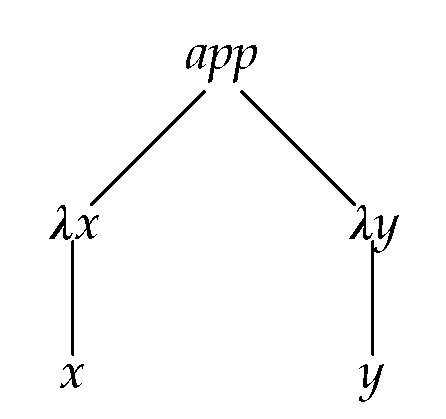
\includegraphics[width=0.3\textwidth]{images/tree}
\caption{Tree structure of the expression $(\lambda x.x) (\lambda y.y)$} \label{fig:tree}
\end{figure}

The untyped $\lambda$-calculus is a rewriting system. 
Redexes are rewritten by replacing free occurences of variables in an expression with another expression.
For instance, the expression $e = (\lambda x.e_1) \: e_2$ can be rewritten as $e = [x \mapsto e_2] e_1$, where $[x \mapsto e_2]$ replaces all free occurences of $x$ in $e_1$ with $e_2$.
A free occurence of a variable is one which is not bound by any abstraction. 
In $e$, the variable $x$ used in $e_1$ refers to the binder $\lambda x$, and as such may be replaced by $e_2$ when applying the substitution $[x \mapsto e_2] e_1$.
When replacing free occurences of $x$ in $e_1$, we have to be careful of \textit{shadowing}, where $e_1$ itself contains an abstraction of $x$ again.
The inner $\lambda$-abstraction ``shadows'' the outer $\lambda$-abstraction.
As a result, not every occurence of $x$ may be replaced within $e_1$, but only the free occurences of $x$.

As shown, the untyped $\lambda$-calculus provides a minimal amount of structure through its grammar. 
In the next section we discuss the simply-typed $\lambda$-calculus, which provides additional structure through its \textit{type system}.

\section{Simply-typed $\lambda$-calculus}
Within the untyped $\lambda$-calculus, a number of expressions are considered valid, but when reduced using $\beta$-reduction will never reach a normal-form.
A normal form is a state where an expression can no longer be rewritten; the computation is finished.
For instance, the expression $\Omega = (\lambda x. x x) (\lambda x. x x)$ will never evaluate to a normal-form.
The expression $Y = \lambda f.( \lambda x.f (x x)) (\lambda x.f (x x))$, named Curry's Y-combinator, allows us to define basic recursion, which also has the ability to never evaluate to a normal-form.

To disallow these non-normalising functions, the simply typed $\lambda$-calculus introduces a type system, where every term has a well-defined type.
The simply typed $\lambda$-calculus is strongly normalizing.
Strongly normalizing implies that every valid expression will reduce to a normal form without exception.
In practice, this is often considered too strict, which is why a fixpoint-combinator can be introduced as a \textit{primitive}.
A primitive is, like the terms of the untyped $\lambda$-calculus, part of the definition of the language.

Since every valid expression reduces to a normal form, every valid expression is known to be terminating, given finite inputs.
As a result, the simply-typed $\lambda$-calculus is \textit{not} turing-complete.
We introduce the grammar of the simply-typed $\lambda$-calculus below, or $\lambda^\rightarrow$ for short.

\begin{definitiontitled}[text only,float]{Grammar of $\lambda^{\rightarrow}$}{def:lambda}
\begin{changemargin}{-0.5cm}{0cm}
\begin{minipage}[b]{0.50\linewidth}
\begin{tabular}{lclr}
e       & $\Coloneqq$ &                             & \textit{expressions:} \\
        & |    & x                                 & \textit{(variable)} \\
        & |    & $\lambda$ x:$\tau$.e              & \textit{(abstraction)} \\
        & |    & e e                               & \textit{(application)} \\
        & |    & c                                 & \textit{(constant)} \\
        & |    & \textbf{let} x = e \textbf{in} e  & \textit{(let binding)} \\
\\
c       & $\Coloneqq$ &                             & \textit{primitive literals} \\
        & |    & true                              & \textit{(Boolean true)} \\
        & |    & false                             & \textit{(Boolean false)} \\
        & |    & n $\in \mathbb{Z}$                & \textit{(Integer literals)} \\
\end{tabular}
%\captionof{table}{Definition of $\lambda$ with explicit data.}
\end{minipage}
\begin{minipage}[b]{0.40\linewidth}
\begin{tabular}{lclr}
$\tau$  & $\Coloneqq$ &                             & \textit{types:} \\
        & |     & $\tau \rightarrow \tau$          & \textit{(function type)} \\
        & |     & T                                & \textit{(base type)} \\
\\
T       & $\Coloneqq$ &                             & \textit{base types:} \\
        & |     & Bool                             & \textit{(Boolean type)} \\
        & |     & Int                              & \textit{(Integer type)} \\
\\
$\Gamma$& $\Coloneqq$ &                             & \textit{contexts:} \\
        & |     & $\emptyset$                      & \textit{(empty context)} \\
        & |     & $\Gamma$,x:T                     & \textit{(term variable binding)} \\
\end{tabular}
%\captionof{table}{Definition of $\lambda_{\rightarrow}$}
\end{minipage}
\end{changemargin}
\end{definitiontitled}

This definition shows the addition of a type $\tau$ to the abstraction expression.
Variables introduced through $\lambda$-abstraction need to have a type annotation, in order for the system to be able to construct the correct function type.
Types have one constructor, namely $\rightarrow$, which constructs a function type from two other types.
Types need to be finite, meaning construction of a type must always terminate.
As a result, every type must, at some point, use base types in its definition.

$\lambda^\rightarrow$ can not express polymorphism.
For instance, the general form of the identity function in the untyped $\lambda$-calculus ($\lambda x.x$), is not valid in $\lambda^\rightarrow$, as $x$ must have a type.
Whenever $x$ has a type, such as in $\lambda x:Int.x$, we can derive the type of the expression.
The $\lambda$-abstraction introduces the $\rightarrow$ constructor, which allows us to create function types using base types.
The function $(\lambda x:Int.x)$ has type $Int \rightarrow Int$, since the type of the result of the identity function has the same type as the function argument.
We will revisit polymorphism in section \ref{sec:polymorphiclambda}.

The type system of $\lambda^\rightarrow$ is not complete without typing rules.
Typing rules express the relation between types and expressions, and in particular define which expressions are \textit{valid} and which are not.
The nature of the typing rules for $\lambda^\rightarrow$ also makes it possible to \textit{(re)construct} the the types from (partial) type information.
We will explain the typing rules of $\lambda^\rightarrow$ next, where we we also explain the meaning of the context $\Gamma$ as introduced by definition \ref{def:lambda}.

\subsection{Typing rules}
In this section we present the typing rules of $\lambda^\rightarrow$, using the commonly used Gentzen style of the sequent calculus\cite{gentzen1935untersuchungen}.
For every valid expression $e$ in $\lambda^\rightarrow$, a single rule expresses the relation between the expression and the type of the expression.
Using these rules, a proof can be constructed for any valid expression $e$ in $\lambda^\rightarrow$, by (de)-constructing the expression using the typing rules.
When a proof cannot be constructed, then the expression is considered invalid.

We use $\tau$ and $\rho$ to range over types.
As is customary in type theory, we use $\Gamma$ to represent the \textit{context} or \textit{type environment}.
$\Gamma$ is a set of pairs, which expresses the relation between \textit{variable names} and \textit{types}, as shown by definition \ref{def:lambda}.
The type environment is needed in order to make judgements based on the context an expression is used in.
For instance, the expression $x + 1$ cannot be typed when nothing is known about $x$. 
We use $\Gamma$ to provide the context in which we can make a statement about $x+1$. 
If $\Gamma = \{ x : \textit{Int}, + : \textit{Int} \rightarrow \textit{Int} \rightarrow \textit{Int} \}$ and we assume that the literal $1$ has type \textit{Int}, then the entire expression would have type \textit{Int} as well.
However, we can only make this judgement when we know the context $\Gamma$ in which the statement $x+1$ is used.

In the typing rules, statements about the context are made explicit by use of the \textit{turnstile} ($\vdash$) symbol.
For instance, $\Gamma \vdash x : \tau$ indicates that the type of $x$ is $\tau$, which is derived from the context $\Gamma$.
The turnstile indicates derivability; we can derive $x : \tau$ from $\Gamma$.
As shown by the typing rules of definition \ref{def:typerulelambda}, typing rules consist of of two parts: the \textit{premise} of the rule, and the \textit{conclusion}.
The premise is separated from the conclusion by a horizontal line, with the premise(s) above the line, while the conclusion is written below the line.

\begin{definitiontitled}[text only]{Typing Rules for $\lambda^\rightarrow$}{def:typerulelambda}
\begin{tabularx}{\textwidth}{ c l X c r}
$ \displaystyle
  \frac
    { }
    { \Gamma, x : \tau \vdash x : \tau }
$ & 
T-Var
&
&
$ \displaystyle
  \frac
    { }
    { c : T }
$
&
T-Const
\\
\\
$ \displaystyle
  \frac
    { \Gamma,x:\rho \vdash e : \tau }
    { \Gamma \vdash \lambda x:\rho.e : \rho \rightarrow \tau}
$
&
T-Abs
&
&
$ \displaystyle
  \frac
    { \Gamma \vdash e_1 : \rho \rightarrow \tau \quad \Gamma \vdash e_2 : \rho }
    { \Gamma \vdash e_1 \: e_2 : \tau }
$
& 
T-App
\\
\end{tabularx}\\
\\

\begin{tabularx}{\textwidth}{X r l X}
 &
$ \displaystyle
  \frac
    { \Gamma \vdash e_1 : \rho \quad \Gamma,x:\rho \vdash e_2 : \tau}
    { \Gamma \vdash \textbf{let } x=e_1 \textbf{ in } e_2 : \tau}
$ 
& 
T-Let
&
\\
\end{tabularx}
\end{definitiontitled}

As shown, both the rules T-Var and T-Const are trivial.
Given a literal ``true'', ``false'' or a natural number, we can conclude that it would have either the type \textit{Bool} or \textit{Int}. 
The rule T-Var is slightly less trivial.
The conclusion $\Gamma, x : \tau \vdash x : \tau$ defines that, whatever the context $\Gamma$ is, when we add $x : \tau$ to it, we can conclude that $x$ does indeed have type $\tau$.
While it may seem that both of these rules can always be applied because there is a lack of a premise, it is really only the case for T-Const.
We can only derive $x : \tau$ in T-Var when $x : \tau$ is part of the context $\Gamma$.
This means that the statement $x + 1$, with the empty context $\varnothing$, does not have a derivable type.
The variable $x$ must be introduced by $\lambda$-abstraction, as defined in the following rule, T-Abs.

The rule T-Abs shows the relation between abstraction and the function type constructor $\rightarrow$.
The context $\Gamma$ is extended with $x:\rho$ when deriving the expression $e$ where $x$ is abstracted from.
From the extended context $\Gamma$ we then derive $e$ has type $\tau$.
When the entire premise $\Gamma, x : \rho \vdash e : \tau$ holds, we derive from the \textit{non-extended} $\Gamma$, that $\lambda x:\rho.e$ has type $\rho \rightarrow \tau$.
With the T-Abs rule, we show how abstraction \textit{introduces} a function type.

Conversely, the T-Abs rule eliminates the $\rightarrow$ type constructor.
The rule T-App has two premises, where both $e_1$ and $e_2$ are derived to have the types $\rho \rightarrow \tau$ and $\rho$ respectively.
Here, when we mention $\rho$, we mean the \textit{same} type in both premises.
This means that the T-Abs rule can only be applied when the left-most expression $e_1$ of application has a function type.
Moreover, the type of the right-most expression $e_2$ must match the argument of the type of $e_1$.
When these premises hold, we may derive $e_1 \: e_2 : \tau$ from the same context $\Gamma$.

Finally, the T-Let rule defines two premises must hold, in order to derive $\textbf{let } x = e_1 \textbf{ in } e_2$ to have type $\tau$.
First, we use the context $\Gamma$ to derive the type of $e_1$ to be $\rho$.
Secondly, we add the type binding $x : \rho$ to $\Gamma$ in order to derive the type of $e_2$.
The type of $x$ must be added to $\Gamma$, as $x$ is (probably) referenced within $e_2$, so in order to derive the type of $e_2$, the context must have that information available.
When both these premises hold, then the entire let-statement has type $\tau$.
As the simply typed $\lambda$-calculus has no polymorphism the use of the let-binding is limited.
In the next section we give an introduction to let-polymorphism and constraint-based typing.

\section{Polymorphic $\lambda$-calculus} \label{sec:polymorphiclambda}
In the simply-typed $\lambda$-calculus, no polymorphic functions can be defined.
A polymorphic function can be seen as a \textit{family} of functions, of which an instance is chosen depending on the context which it is used in.
As a trivial example, consider the identity function $\lambda x.x$.
The identity function in the untyped $\lambda$-calculus does not have a notion of types, and can therefor be applied to any value.
This is not the case in the simply-typed $\lambda$-calculus, but we can define the set of all functions which \textit{share} the definition of the identity function under type-erasure.
Both the functions $(\lambda x : \textit{Int}. x) : \textit{Int} \to \textit{Int}$ and $(\lambda x : \textit{Bool}.x) : \textit{Bool} \to \textit{Bool}$ share the same definition.
While this makes intuitive sense, it is not a trivial problem for a type system to solve.
\citeauthor{wand1987simple} defines\cite{wand1987simple} the problem of polymorphism as ``Given a term of the untyped $\lambda$-calculus, to find all terms of the typed $\lambda$-calculus which yield the given term when the type information on bound variables is deleted.''
In effect, when we have an expression of the untyped $\lambda$-calculus, we try to find the \textit{family} of valid types belonging to that expression.

To show how this is done, we first extend the grammar of $\lambda^\rightarrow$.
Secondly, we introduce polytypes, which allow us to reason about polymorphic types.
Using polytypes, we define what constitutes the most general type of an expression, known as the principal type. 
Finally, using principal types and polytypes, we show how the process of type-checking is split in two by using \textit{constraints}.
To do so, we focus on the well-known ``Damas-Milner''\cite{damas1982principal} type reconstruction algorithm, which is also known as the ``Hindley-Milner'' or ``Damas-Hindley-Milner'' type reconstruction algorithm.
%We also briefly look at the type system of ``Parameterized Hindley-Milner''\cite{odersky1999type}, also known as HM(X), to show how constraints can be represented in typing rules.
%HM(X) is considered\cite{pierce2005advanced} an extension of the type system of Damas-Milner, which is why our discussion of it will only be very brief.

\subsection{Principal Types}
We focus on principal types first.
We extend the grammar of $\lambda^\rightarrow$ with type variables.
This leads to the grammar we call $\lambda_{DM}$, which is shown by definition \ref{def:lambdaconstraint}.
The rest of the grammar is identical to $\lambda^\rightarrow$ from definition \ref{def:typerulelambda}.
As we are introducing polymorphism to the simply typed $\lambda$-calculus, we need a mechanism to introduce polymorphic functions.
For this we use \textit{let-polymorphism} as introduced\cite{milner1978theory} by \citeauthor{milner1978theory}. 
There, let-bindings are used to introduce polymorphic functions, which can be used multiple times within the body of the let-binding, regardless of possible conflicting types between each instance.
We discuss the idea of let-polymorphism in greater detail later in this section.

\begin{definitiontitled}[text only,float]{Grammar of $\lambda_{DM}$ (Extended from definition \ref{def:lambda}).}{def:lambdaconstraint}
\begin{tabular}{lclr}
$\tau$  & $\Coloneqq$ & $\alpha$          &\textit{(type variable)}\\
        & |          & $\ldots$          & \\
\\
$e$     & $\Coloneqq$ & $\lambda x.e$     &\textit{(abstraction)} \\
        & |           & \ldots           & \\
\end{tabular}
\end{definitiontitled}

Aside from using $\alpha$ for type variables, we also use $\beta$ when two type variables are distinctly different.
Type variables in $\lambda_{DM}$ are \textit{monomorphic}, meaning a type variable can only refer to a single type.
Moreover, without further modification, all type variables are \textit{free} variables, as they are not bound to abstraction like term variables in the $\lambda$-calculus.
Type variables are used in \textit{polytypes}\footnote{Some authors, such as \citeauthor{milner1978theory}, prefer to use the term \textit{type scheme}. Here, we use the term polytype.}, shown by definition \ref{def:typescheme}.
Polytypes make it possible to introduce \textit{polymorphism} using monomorphic type variables. 

\begin{definitiontitled}[text only,float]{Polytypes}{def:typescheme}
A polytype $\sigma$ is defined by universal quantification over a finite number of type variables:
\[
\sigma = \forall \alpha_0,\alpha_1, \ldots, \alpha_n. \tau \quad (n \ge 0)
\]
, where the type variables $\alpha_0$ to $\alpha_n$ are considered bound within $\tau$.
\end{definitiontitled}

Polytypes consist of universal quantification over type variables.
The type variables used by universal quantification are bound within the polytype $\sigma$.
In the polytype $\sigma = \forall \varnothing.\tau$, the polytype $\sigma$ is equal to the type $\tau$.
Whenever a substitution of the form $[\alpha \mapsto \rho]$ is applied to a polytype $\sigma$, the resulting type is called an \textit{instance} of $\sigma$.
Similarly, a \textit{set} of substitutions $S$ may be applied to $\sigma$.

We can use polytypes to define polymorphic functions.
For instance, the identity function $\lambda x.x$ is polymorphic when it has the associated polytype $\sigma = \forall \alpha. \alpha \rightarrow \alpha$.
When applied to a value, for instance $1 : \textit{Int}$, the substitution $[\alpha \mapsto Int]$ can be applied to $\sigma$, leading to the type instance $\sigma = \forall \varnothing. \textit{Int} \rightarrow \textit{Int}$.

As shown, we can create an instance of a polytype by applying a substitution to a polytype.
Given the identity function, there exist many different substitutions to create type instances of the associated polytype.
For instance, the identity function, when associated with polytype $\sigma = \forall \alpha. \alpha \rightarrow \alpha$, can be instantiated using the substitutions $[\alpha \mapsto \textit{Bool}]$, $[\alpha \mapsto \textit{Int}]$, or even $[\alpha \mapsto (\textit{Int} \rightarrow \textit{Bool})]$ and other variations.
Given that many substitutions exists, the principal type is defined informally as the type which is least constricting, but is still a valid type.
That is, the principal type $\tau$ of an expression $e$, is the type to which any set of substitutions may be applied, assuming the set of substitutions lead to a valid type $\tau'$ of $e$.

\begin{definitiontitled}[text only,float]{Principal Types}{def:principal}
Given a type $\tau$, associated with a polytype $\sigma = \forall \alpha_0, \alpha_1 \ldots \alpha_n. \tau$ of an expression $e$, then $\tau$ is the principal type of $e$ iff:
\begin{enumerate}
 \item the type $\tau$ holds under the empty context, that is, $\varnothing \vdash e : \tau$;
 \item $\forall \tau'. \varnothing \vdash e : \tau' \Rightarrow \exists S.\tau' = S\tau$, that is, for all valid types $\tau'$ of $e$, there exists a set of substitutions $S$, such that $\tau$ can be turned into $\tau'$.
\end{enumerate}
\end{definitiontitled}

In some of the literature the binary relation $\sqsubseteq$ is defined as well.
This relation is used to express an ordering in polytypes.
Given two polytypes $\sigma' \sqsubseteq \sigma$ defines $\sigma'$ to be at least as constricting as $\sigma$.
For instance, given $(\sigma' = \forall \alpha. \textit{Int} \to \alpha)$ and $(\sigma = \forall \alpha,\beta. \beta \to \alpha)$, the relation $\sigma' \sqsubseteq \sigma$ holds.
Similarly, $\sigma \sqsubseteq \sigma$ holds, as $\sigma$ is at least as constricting as itself.

\begin{definitiontitled}[text only]{Typing Rules for $\lambda_{DM}$}{def:dmrules}
\begin{tabularx}{\textwidth}{ c l X c r}
$ \displaystyle
  \frac
    { \Gamma(x) = \sigma }
    { \Gamma \vdash x : \sigma }
$ & 
DM-Var
&
&
$ \displaystyle
  \frac
    { }
    { \varnothing \vdash c : T }
$
&
DM-Const
\\
\\
$ \displaystyle
  \frac
    { \Gamma,x:\rho \vdash e : \tau }
    { \Gamma \vdash \lambda x:\rho.e : \rho \rightarrow \tau}
$
&
DM-Abs
&
&
$ \displaystyle
  \frac
    { \Gamma \vdash e_1 : \rho \rightarrow \tau \quad \Gamma \vdash e_2 : \rho }
    { \Gamma \vdash e_1 \: e_2 : \tau }
$
& 
DM-App
\\
\\
$ \displaystyle
  \frac
  { \Gamma \vdash t : \sigma \quad \alpha \notin \textit{ftv}(\Gamma) }
  { \Gamma \vdash e : \forall \alpha.\sigma }
$
&
DM-Gen
& 
& 
$ \displaystyle
  \frac
  { \Gamma \vdash e : \sigma \quad \sigma' \sqsubseteq \sigma }
  { \Gamma \vdash e : \forall \alpha.\sigma' }
$
&
DM-Inst
\\
\end{tabularx}\\
\\

\begin{tabularx}{\textwidth}{X r l X}
 &
$ \displaystyle
  \frac
    { \Gamma \vdash e_1 : \sigma \quad \Gamma,x:\sigma \vdash e_2 : \tau}
    { \Gamma \vdash \textbf{let } x=e_1 \textbf{ in } e_2 : \tau}
$ 
& 
DM-Let
&
\\
\end{tabularx}
\end{definitiontitled}

Using principal types, we define the typing rules of the Damas-Milner type system in definition \ref{def:dmrules}.
Most of the rules of the Damas-Milner type system are straightforward.
The rules DM-Abs and DM-App are exactly the same as the rules T-Abs and T-App from page \pageref{def:typerulelambda}.
However, instead of binding the type of a variable $x$ to $\tau$ in the rule DM-Var, the type of a variable is bound to a polytype.
This is a conservative extension, as polytypes allow expression of not-polymorphic types.
This does \textit{not} mean higher order polymorphic functions are allowed, as abstraction has no notion of a polytype.
Instead, polymorphic functions can only be introduced by the rule DM-Let.
DM-let defines that, given an expression $e_1$, associated with polytype $\sigma$, $e_1$ may be used in $e_2$, but only if it leads to $e_2$ having a monotype $\tau$.
This is called \textit{let-polymorphism}, as introduced earlier.

Two other rules are needed in order to both \textit{introduce} and \textit{eliminate} polymorphic type variables.
The rules DM-Gen and DM-Inst do just that.
The rule DM-Gen allows introduction of universal quantification, but only if the type variable $\alpha$ used in universal quantification is bound in the context $\Gamma$. 
This is indicated by the meta-function \textit{ftv}, which determines the \textit{free type variables} of its argument.
The rule DM-Inst allows instantiation of a polytype (e.g. apply a valid substitution to a polytype), provided the new polytype $\sigma'$ is at least as constricting as the original polytype $\sigma$.
By carefully allowing polytypes in only part of the typing rules of DM, polymorphic types can \textit{never} be substituted with other polymorphic types\cite{pierce2002types}.
This form of polymorphism is called predicative polymorphism, as opposed to the impredicative polymorphism of for instance System F\cite{girard1971extension}.


\subsection{Type-checking using Polytypes}
Principal types make it difficult to check the types of expressions using a syntax-directed approach.
In a syntax-directed approach, type-checking can be done \textit{solely} by applying typing rules.
When no typing rule applies, the expression being checked does not have a valid type.
When the entire expression is checked, the entire expression has a valid type, provided the type system is sound.

However, to type-check expressions containing polytypes, that approach is not as straightforward.
It is difficult to express the concept of principal types, and how to derive a set of substitutions for that principal type, using a syntax-directed approach.
The typing rules of \citeauthor{damas1982principal} ``do not provide an easy method for finding, given a context $\Gamma$ and expression $e$, a polytype $\sigma$ such that $\Gamma \vdash e : \sigma$.''\cite{damas1982principal}
\citeauthor{milner1978theory} provides the $W$ algorithm to find a polytype $\sigma$, given a context $\Gamma$ and an expression $e$.
The algorithm, which is presented in full detail later, uses \citeauthor{robinson1965machine}'s Unification\cite{robinson1965machine} algorithm to find the most general type possible for every expression and declaration.
Algorithm W was later reformulated by \citeauthor{damas1982principal} in ``Principal Type-schemes for Functional Programs''\cite{damas1982principal}.
Essentially, algorithm $W$ interleaves generation and unification of \textit{type constraints} to find the most general type of a given expression.

\begin{definitiontitled}[text only,float]{Algorithm W}{def:algorithmw}
\[
\begin{array}{l c l}
W(\Gamma,x)           & = & \text{let } \Gamma(x) = \forall \alpha_1,\ldots,\alpha_n.\tau' \\ 
                      &   & \text{and } \beta_i \notin \Gamma \\
                      &   & \text{in } (\{\},[\beta_i/\alpha_i]\tau') \\
W(\Gamma,e_1 \: e_2)  & = & \text{let }   (S_1,\tau_1) = W(\Gamma, e_1)\\
                      &   & \text{and }   (S_2,\tau_2) = W(S_1 \Gamma, e_2)\\
                      &   & \text{and }   V            = \textit{unify}(\{S_2\tau_1 = \tau_2 \to \beta\}) \\
                      &   & \text{and }   \beta \notin \Gamma \\
                      &   & \text{in }    (V \cup S_2 \cup S_1, V \beta) \\
W(\Gamma,\lambda x.e) & = & \text{let }   (S,\tau) = W((\Gamma,x:\beta),e)\\
                      &   & \text{and }   \beta \notin \Gamma \\ 
                      &   & \text{in }    (S, S\beta \to \tau) \\
W(\Gamma,\textbf{let } x = e_1 \textbf{ in } e_2) & = & \text{let } (S_1,\tau_1) = W(\Gamma,e_1) \\
                                                  &   & \text{and   } (S_2,\tau_2) = W((S_1\Gamma,x : \forall \alpha_1,\ldots,\alpha_n.\tau_1, e_2) \\
                                                  &   & \text{and   } \{ \alpha_1, \ldots, \alpha_n \} = \textit{ftv}(\tau_1) \textbackslash \textit{ftv}(S_1\Gamma) \\
                                                  &   & \text{in } (S_2 \cup S_1, \tau_2) \\
\end{array}
\]
\end{definitiontitled}

We now discuss algorithm $W$ (definition \ref{def:algorithmw}).
Given a context $\Gamma$ and expression $e$, the algorithm returns a set of substitutions $S$ and a type $\tau$, such that $S\Gamma \vdash \tau$.
Depending on the expression, the algorithm defines a different procedure to derive the principal type of the expression.
In the case of a variable, all type variables bound in the polytype of $x$ are replaced by fresh type variables.
Type variables are replaced using $\alpha$-conversion, and as such the set of substitutions returned is empty.

When one expression $e_1$ is applied to another expression $e_2$, the set of substitutions $S_1$ and type $\tau_1$ of $e_1$ is derived by applying the $W$ algorithm recursively.
The resulting substitutions are then applied to $\Gamma$, in order to derive the set of substitutions $S_2$ and most general type $\tau_2$ of $e_2$.
Finally, the unification algorithm is used to find a set of substitutions $V$, such that $S_1 \tau_1 = \tau_2 \to \beta$, where $\beta$ is a fresh type variable.
The unification algorithm, which is not shown here, accepts a constraint of the form $\tau = \tau'$, and results in a set of substitutions such that $V\tau = \tau'$, if such a set exists.
The constraint $S_1 \tau_1 = \tau_2 \to \beta$ makes it clear that the type of $e_2$ has to agree with the type of the first argument of $e_1$.
If this is the case, then $e_1 \: e_2$ is defined to have type $\beta$, which is subject to the resulting substitutions $V$ from the unification algorithm.

In the case of a $\lambda$-abstraction, a fresh type variable $\beta$ is introduced as the type of the argument $x$.
The context $\Gamma$, together with the body $e$ of the $\lambda$-abstraction, is supplied to $W$ to define the set of substitutions $S$ and principal type $\tau$, such that the type of $\lambda x.e$ is $S\beta \to \tau$.

Lastly, in the case of a let-binding, the most general type of the binding is found.
The substitutions $S_1$, together with type $\tau_1$, are then used to modify the context $\Gamma$, which is used to derive the most general type of $e_2$.
The polytype used to append $\Gamma$ to derive $e_2$ binds the variables which are unique in $\textit{ftv}(\tau_1)$, when compared to the type variables of $\textit{ftv}(S_1\Gamma)$. 
If this were not done, then referencing $x$ in $e_2$ would create fresh variables for type variables which are already substituted in $\Gamma$.

\section{Conclusion}
The type systems discussed in this chapter show how we can reason about properties of (certain expressions of) the $\lambda$-calculus.
The type system of Damas-Milner shows that, in order to reason about more complex types, type-checking can be done in two steps.
As a result, the type system of Damas-Milner is not complete by only giving the typing rules.
The typing rules are used to (re)construct types, but do not have the ability to determine principal types.
For this the $W$ algorithm is introduced.
We consider both algorithm $W$ and the typing rules to make up the entire type system of Damas-Milner.

In the same vein, we define our own type system in two steps in the next chapters as well.
Like Damas-Milner, the typing rules lead to a number of constraints.
Instead of defining the constraint generation in a separate algorithm however, we use the same approach as HM(X)\cite{odersky1999type}, which is considered\cite{pierce2005advanced} an extension of the type system of Damas-Milner.
Discussion of this type system is out of the scope of this thesis however, as we have no specific interest in the general polymorphism described by the HM(X) type system.


%% ODER: format ==         = "\mathrel{==}"
%% ODER: format /=         = "\neq "
%
%
\makeatletter
\@ifundefined{lhs2tex.lhs2tex.sty.read}%
  {\@namedef{lhs2tex.lhs2tex.sty.read}{}%
   \newcommand\SkipToFmtEnd{}%
   \newcommand\EndFmtInput{}%
   \long\def\SkipToFmtEnd#1\EndFmtInput{}%
  }\SkipToFmtEnd

\newcommand\ReadOnlyOnce[1]{\@ifundefined{#1}{\@namedef{#1}{}}\SkipToFmtEnd}
\DeclareFontFamily{OT1}{cmtex}{}
\DeclareFontShape{OT1}{cmtex}{m}{n}
  {<5><6><7><8>cmtex8
   <9>cmtex9
   <10><10.95><12><14.4><17.28><20.74><24.88>cmtex10}{}
\DeclareFontShape{OT1}{cmtex}{m}{it}
  {<-> ssub * cmtt/m/it}{}
\newcommand{\texfamily}{\fontfamily{cmtex}\selectfont}
\DeclareFontShape{OT1}{cmtt}{bx}{n}
  {<5><6><7><8>cmtt8
   <9>cmbtt9
   <10><10.95><12><14.4><17.28><20.74><24.88>cmbtt10}{}
\DeclareFontShape{OT1}{cmtex}{bx}{n}
  {<-> ssub * cmtt/bx/n}{}
\newcommand{\tex}[1]{\text{\texfamily#1}}	% NEU

\newcommand{\Sp}{\hskip.33334em\relax}


\newcommand{\Conid}[1]{\mathit{#1}}
\newcommand{\Varid}[1]{\mathit{#1}}
\newcommand{\anonymous}{\kern0.06em \vbox{\hrule\@width.5em}}
\newcommand{\plus}{\mathbin{+\!\!\!+}}
\newcommand{\bind}{\mathbin{>\!\!\!>\mkern-6.7mu=}}
\newcommand{\rbind}{\mathbin{=\mkern-6.7mu<\!\!\!<}}% suggested by Neil Mitchell
\newcommand{\sequ}{\mathbin{>\!\!\!>}}
\renewcommand{\leq}{\leqslant}
\renewcommand{\geq}{\geqslant}

%mathindent has to be defined
\@ifundefined{mathindent}%
  {\newdimen\mathindent\mathindent\leftmargini}%
  {}%

\def\resethooks{%
  \global\let\SaveRestoreHook\empty
  \global\let\ColumnHook\empty}
\newcommand*{\savecolumns}[1][default]%
  {\g@addto@macro\SaveRestoreHook{\savecolumns[#1]}}
\newcommand*{\restorecolumns}[1][default]%
  {\g@addto@macro\SaveRestoreHook{\restorecolumns[#1]}}
\newcommand*{\aligncolumn}[2]%
  {\g@addto@macro\ColumnHook{\column{#1}{#2}}}

\resethooks

\newcommand{\onelinecommentchars}{\quad-{}- }
\newcommand{\commentbeginchars}{\enskip\{-}
\newcommand{\commentendchars}{-\}\enskip}

\newcommand{\visiblecomments}{%
  \let\onelinecomment=\onelinecommentchars
  \let\commentbegin=\commentbeginchars
  \let\commentend=\commentendchars}

\newcommand{\invisiblecomments}{%
  \let\onelinecomment=\empty
  \let\commentbegin=\empty
  \let\commentend=\empty}

\visiblecomments

\newlength{\blanklineskip}
\setlength{\blanklineskip}{0.66084ex}

\newcommand{\hsindent}[1]{\quad}% default is fixed indentation
\let\hspre\empty
\let\hspost\empty
\newcommand{\NB}{\textbf{NB}}
\newcommand{\Todo}[1]{$\langle$\textbf{To do:}~#1$\rangle$}

\EndFmtInput
\makeatother
%
%
%
%
%
%
% This package provides two environments suitable to take the place
% of hscode, called "plainhscode" and "arrayhscode". 
%
% The plain environment surrounds each code block by vertical space,
% and it uses \abovedisplayskip and \belowdisplayskip to get spacing
% similar to formulas. Note that if these dimensions are changed,
% the spacing around displayed math formulas changes as well.
% All code is indented using \leftskip.
%
% Changed 19.08.2004 to reflect changes in colorcode. Should work with
% CodeGroup.sty.
%
\ReadOnlyOnce{polycode.fmt}%
\makeatletter

\newcommand{\hsnewpar}[1]%
  {{\parskip=0pt\parindent=0pt\par\vskip #1\noindent}}

% can be used, for instance, to redefine the code size, by setting the
% command to \small or something alike
\newcommand{\hscodestyle}{}

% The command \sethscode can be used to switch the code formatting
% behaviour by mapping the hscode environment in the subst directive
% to a new LaTeX environment.

\newcommand{\sethscode}[1]%
  {\expandafter\let\expandafter\hscode\csname #1\endcsname
   \expandafter\let\expandafter\endhscode\csname end#1\endcsname}

% "compatibility" mode restores the non-polycode.fmt layout.

\newenvironment{compathscode}%
  {\par\noindent
   \advance\leftskip\mathindent
   \hscodestyle
   \let\\=\@normalcr
   \let\hspre\(\let\hspost\)%
   \pboxed}%
  {\endpboxed\)%
   \par\noindent
   \ignorespacesafterend}

\newcommand{\compaths}{\sethscode{compathscode}}

% "plain" mode is the proposed default.
% It should now work with \centering.
% This required some changes. The old version
% is still available for reference as oldplainhscode.

\newenvironment{plainhscode}%
  {\hsnewpar\abovedisplayskip
   \advance\leftskip\mathindent
   \hscodestyle
   \let\hspre\(\let\hspost\)%
   \pboxed}%
  {\endpboxed%
   \hsnewpar\belowdisplayskip
   \ignorespacesafterend}

\newenvironment{oldplainhscode}%
  {\hsnewpar\abovedisplayskip
   \advance\leftskip\mathindent
   \hscodestyle
   \let\\=\@normalcr
   \(\pboxed}%
  {\endpboxed\)%
   \hsnewpar\belowdisplayskip
   \ignorespacesafterend}

% Here, we make plainhscode the default environment.

\newcommand{\plainhs}{\sethscode{plainhscode}}
\newcommand{\oldplainhs}{\sethscode{oldplainhscode}}
\plainhs

% The arrayhscode is like plain, but makes use of polytable's
% parray environment which disallows page breaks in code blocks.

\newenvironment{arrayhscode}%
  {\hsnewpar\abovedisplayskip
   \advance\leftskip\mathindent
   \hscodestyle
   \let\\=\@normalcr
   \(\parray}%
  {\endparray\)%
   \hsnewpar\belowdisplayskip
   \ignorespacesafterend}

\newcommand{\arrayhs}{\sethscode{arrayhscode}}

% The mathhscode environment also makes use of polytable's parray 
% environment. It is supposed to be used only inside math mode 
% (I used it to typeset the type rules in my thesis).

\newenvironment{mathhscode}%
  {\parray}{\endparray}

\newcommand{\mathhs}{\sethscode{mathhscode}}

% texths is similar to mathhs, but works in text mode.

\newenvironment{texthscode}%
  {\(\parray}{\endparray\)}

\newcommand{\texths}{\sethscode{texthscode}}

% The framed environment places code in a framed box.

\def\codeframewidth{\arrayrulewidth}

\newenvironment{framedhscode}%
  {\parskip=\abovedisplayskip\par\noindent
   \hscodestyle
   \arrayrulewidth=\codeframewidth
   \tabular{@{}|p{\linewidth-2\arraycolsep-2\arrayrulewidth-2pt}|@{}}%
   \hline\framedhslinecorrect\\{-1.5ex}%
   \let\endoflinesave=\\
   \let\\=\@normalcr
   \(\pboxed}%
  {\endpboxed\)%
   \framedhslinecorrect\endoflinesave{.5ex}\hline
   \endtabular
   \parskip=\belowdisplayskip\par\noindent
   \ignorespacesafterend}

\newcommand{\framedhslinecorrect}[2]%
  {#1[#2]}

\newcommand{\framedhs}{\sethscode{framedhscode}}

% The inlinehscode environment is an experimental environment
% that can be used to typeset displayed code inline.

\newenvironment{inlinehscode}%
  {\(\def\column##1##2{}%
   \let\>\undefined\let\<\undefined\let\\\undefined
   \newcommand\>[1][]{}\newcommand\<[1][]{}\newcommand\\[1][]{}%
   \def\fromto##1##2##3{##3}%
   \def\nextline{}}{\) }%

\newcommand{\inlinehs}{\sethscode{inlinehscode}}

% The joincode environment is a separate environment that
% can be used to surround and thereby connect multiple code
% blocks.

\newenvironment{joincode}%
  {\let\orighscode=\hscode
   \let\origendhscode=\endhscode
   \def\endhscode{\def\hscode{\endgroup\def\@currenvir{hscode}\\}\begingroup}
   %\let\SaveRestoreHook=\empty
   %\let\ColumnHook=\empty
   %\let\resethooks=\empty
   \orighscode\def\hscode{\endgroup\def\@currenvir{hscode}}}%
  {\origendhscode
   \global\let\hscode=\orighscode
   \global\let\endhscode=\origendhscode}%

\makeatother
\EndFmtInput
%

\chapter{Specification of Time-dependent Behaviour} \label{ch:specification}
In the previous chapter, we discussed different type systems of the $\lambda$-calculus.
As stated in the introduction, the primary goal of this thesis is to provide a type system, which can be used to specify and verify time-dependent behaviour.
To make it easier to digest the definition of the type system, we split discussion of the type system in two parts.
First, we focus on the specification of time-dependent behaviour.
We do this by discussing how the type system of Haskell is currently used in \gls{clash}, after which we discuss how our type system can be used to more concisely specify time-dependent behaviour than currently possible.
Secondly, we focus on the grammar and typing rules of our type system in the next chapter.
The order in which these two chapters are read, is not very important.
As such, for readers more interested in the definition of the type system, the next chapter may be read before this one.

The type systems introduced in the previous chapter were not specifically created for hardware design.
To show how traditional type systems are used in the context of hardware design, we give a brief introduction as to how the type system of Haskell is currently used in \gls{clash}.
\gls{clash} leverages the language Haskell, which means it adopts the syntax of the language, together with the type system and other parts of the \gls{ghc} in order to generate \gls{vhdl} code.
As such an understanding of the Haskell language is preferred in order to read this chapter, though the basic syntax of the language is discussed as well.
If such understanding is limited or non-existent, \citeauthor{o2009real} have written\cite{o2009real} an excellent, freely available introduction to Haskell and its syntax.

After the brief introduction to the type system of \gls{clash} and how \gls{clash} can be used to define time-dependent behaviour, we introduce a different method of specifying the same behaviour.
Following, we discuss how type reconstruction is used to derive the time-dependent behaviour of compositions.
Finally, we discuss sequences, and how sequences are reasoned about in the type system.

%%%%%%%%%%%%%%%%%%%%%
%
% Combinational Logic
%
%%%%%%%%%%%%%%%%%%%%%
\section{Specification of Combinational Logic}
In \gls{clash}, combinational logic is represented through pure functions.
Like combinational logic, pure functions only affect the values they are applied to; they are side-effect free.
For instance, the combinational logic of figure \ref{fig:combinational1} is represented as a pure function.

\begin{figure}[H]
\begin{center}
\begin{circuitikz} \draw
(0,2) node[and port] (myand1) {}
(myand1.in 1) node[left] { $ x1 $ }
(myand1.in 2) node[left] { $ x2 $ }
(0,0) node[and port] (myand2) {}
(myand2.in 1) node[left] { $ x3 $ }
(myand2.in 2) node[left] { $ x4 $ }
(2,1) node[xnor port] (myxnor) {}
(myxnor.in 1) node[left] { $ s $ }
(myxnor.in 2) node[left] { $ t $ }
(myxnor.out) node[right] { $ z $ }
(myand1.out) -- (myxnor.in 1)
(myand2.out) -- (myxnor.in 2);
\end{circuitikz}
\end{center}
\caption{A circuit consisting of a few logic gates.} \label{fig:combinational1}
\end{figure}

\gls{clash} is a structural \gls{hdl}.
The structure of the circuit is represented by the expression of the language.
The component from figure \ref{fig:combinational1} can be structurally defined in \gls{clash} through the function \ensuremath{\Varid{combLogic}}.
\begin{texexptitled}[text only]{Combinational logic in \gls{clash} (a).}{code:comblogic}\begin{hscode}\SaveRestoreHook
\column{B}{@{}>{\hspre}l<{\hspost}@{}}%
\column{3}{@{}>{\hspre}l<{\hspost}@{}}%
\column{5}{@{}>{\hspre}l<{\hspost}@{}}%
\column{9}{@{}>{\hspre}l<{\hspost}@{}}%
\column{E}{@{}>{\hspre}l<{\hspost}@{}}%
\>[3]{}\Varid{combLogic}\;\Varid{x1}\;\Varid{x2}\;\Varid{x3}\;\Varid{x4}\mathrel{=}\Varid{z}{}\<[E]%
\\
\>[3]{}\hsindent{2}{}\<[5]%
\>[5]{}\mathbf{where}{}\<[E]%
\\
\>[5]{}\hsindent{4}{}\<[9]%
\>[9]{}\Varid{s}\mathrel{=}\Varid{hwand}\;\Varid{x1}\;\Varid{x2}{}\<[E]%
\\
\>[5]{}\hsindent{4}{}\<[9]%
\>[9]{}\Varid{t}\mathrel{=}\Varid{hwand}\;\Varid{x3}\;\Varid{x4}{}\<[E]%
\\
\>[5]{}\hsindent{4}{}\<[9]%
\>[9]{}\Varid{z}\mathrel{=}\Varid{hwnot}\;(\Varid{hwxor}\;\Varid{s}\;\Varid{t}){}\<[E]%
\ColumnHook
\end{hscode}\resethooks
\end{texexptitled}

As shown by the variables used in \ensuremath{\Varid{combLogic}} and figure \ref{fig:combinational1}, there is an immediate relationship between the code and the structure of the circuit the code represents.
The defined function is named \ensuremath{\Varid{combLogic}} and accepts four arguments.
These arguments are used in the \ensuremath{\mathbf{where}} clause, which allows us to decompose the structure of a single component into multiple sub-components.
Decomposition of the structure in smaller parts makes it easier to see the structure of the circuit.
The \ensuremath{\mathbf{where}} clause introduces variables \ensuremath{\Varid{s}} and \ensuremath{\Varid{t}}, which relate to values transferred between logic gates, while the variable \ensuremath{\Varid{z}} represents the output of the circuit.
The definition of \ensuremath{\Varid{combLogic}} also shows us the influence Haskell has on \gls{clash}.
As function identifiers like \ensuremath{\Varid{and}}, \textit{not} and \ensuremath{\Varid{xor}} are already defined by the Haskell language, \gls{clash} introduces different identifiers like \ensuremath{\Varid{hwand}}, \ensuremath{\Varid{hwnot}}, et cetera, for these functions.

In the definition of \ensuremath{\Varid{combLogic}}, the \ensuremath{\mathbf{where}} clause creates \textit{local} definitions.
We need to be able to detect when something is defined locally, and when something is defined globally, as \ensuremath{\Varid{s}} and \ensuremath{\Varid{t}} should not exist within the same scope as \ensuremath{\Varid{combLogic}}.
The definitions of \ensuremath{\Varid{s}} and \ensuremath{\Varid{t}} only make sense within the scope of \ensuremath{\Varid{combLogic}} after all.
The \textit{off-side rule} allows us to determine when a certain scope ends.
In the definition of \ensuremath{\Varid{combLogic}}, the indentation of the \ensuremath{\mathbf{where}} close defines that \ensuremath{\Varid{s}},\ensuremath{\Varid{t}} and \ensuremath{\Varid{z}} belong to a different scope than \ensuremath{\Varid{combLogic}} itself.

%%%%
% Types in clash
%%%%
\subsection{Types in \gls{clash}}
Functions such as \ensuremath{\Varid{combLogic}} have known types, even if we do not write them down explicitly.
The type system of \gls{clash} can, similar to the type systems of the previous chapter, reconstruct the types of expressions.
The type system of \gls{clash} can infer, from the definition of \ensuremath{\Varid{combLogic}}, that the function only works for values of the type \ensuremath{\Conid{Bit}}.
The \ensuremath{\Conid{Bit}} type is represented by a single wire in a circuit, since a \ensuremath{\Conid{Bit}} only has two values.

Types can also be used in the definition of circuits directly.
Including types in the definition increases clarity and conveys the intent of the designer to the type system.
For instance, the definition of \ensuremath{\Varid{combLogic}} given earlier, is equivalent to the definition of code snippet \ref{code:comblogic2}.

\begin{texexptitled}[text only]{Combinational logic in \gls{clash} (b).}{code:comblogic2}\begin{hscode}\SaveRestoreHook
\column{B}{@{}>{\hspre}l<{\hspost}@{}}%
\column{6}{@{}>{\hspre}l<{\hspost}@{}}%
\column{10}{@{}>{\hspre}l<{\hspost}@{}}%
\column{E}{@{}>{\hspre}l<{\hspost}@{}}%
\>[B]{}\Varid{combLogic}\mathbin{::}\Conid{Bit}\to (\Conid{Bit}\to (\Conid{Bit}\to (\Conid{Bit}\to \Conid{Bit}))){}\<[E]%
\\
\>[B]{}\Varid{combLogic}\;\Varid{x1}\;\Varid{x2}\;\Varid{x3}\;\Varid{x4}\mathrel{=}(\Varid{hwnot}\;(\Varid{hwxor}\;\Varid{s}\;\Varid{t})){}\<[E]%
\\
\>[B]{}\hsindent{6}{}\<[6]%
\>[6]{}\mathbf{where}{}\<[E]%
\\
\>[6]{}\hsindent{4}{}\<[10]%
\>[10]{}\Varid{s}\mathrel{=}\Varid{hwand}\;\Varid{x1}\;\Varid{x2}{}\<[E]%
\\
\>[6]{}\hsindent{4}{}\<[10]%
\>[10]{}\Varid{t}\mathrel{=}\Varid{hwand}\;\Varid{x3}\;\Varid{x4}{}\<[E]%
\ColumnHook
\end{hscode}\resethooks
\end{texexptitled}

The \ensuremath{\mathbin{::}} operator is used to inform the type system of the relation between the identifier \ensuremath{\Varid{combLogic}} and the type \ensuremath{\Conid{Bit}\to (\Conid{Bit}\to (\Conid{Bit}\to (\Conid{Bit}\to \Conid{Bit})))}.
This operation is called ascription and is used to give the type system additional information. 
In functional languages functions are values as well, and as such are also represented by the type system.
The type constructor \ensuremath{\to } constructs a function type from two other value types.
In functional languages, including \gls{clash}, functions are first class, meaning functions are also values.
In the definition of \ensuremath{\Varid{combLogic}}, the type \ensuremath{\Conid{Bit}\to (\Conid{Bit}\to (\Conid{Bit}\to (\Conid{Bit}\to \Conid{Bit})))} represents that, after applying \ensuremath{\Varid{combLogic}} to a valid value of type \ensuremath{\Conid{Bit}}, the function will return another function of type \ensuremath{\Conid{Bit}\to (\Conid{Bit}\to (\Conid{Bit}\to \Conid{Bit}))}.
After the function is applied four times to valid values, the function returns a value of type \ensuremath{\Conid{Bit}}.
The type constructor \ensuremath{\to } is right associative.
This means that a type as \ensuremath{\Conid{Bit}\to \Conid{Bit}\to \Conid{Bit}} is interpreted as \ensuremath{\Conid{Bit}\to (\Conid{Bit}\to \Conid{Bit})}.

\begin{figure}[H]
\begin{center}
\centering
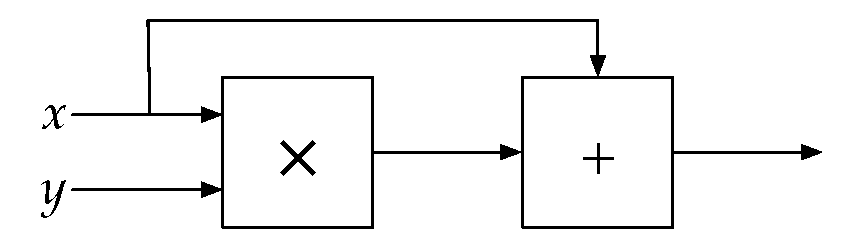
\includegraphics[width=0.5\textwidth]{images/muladd}
\end{center}
\caption{Multiplication and addition combined} \label{fig:muladd}
\end{figure}

Although \gls{clash} allows us to create compositions using combinational logic, not every composition is considered correct.
When the types of a composition do not match, the composition is rejected and a type error is raised.
For instance, using the multiplication operation and addition operation, we combine the two as a function named \ensuremath{\Varid{mulAdd}}.
This is shown below by code snippet \ref{code:combcomposition} to create the circuit of figure \ref{fig:muladd}.
We can not combine the definition of \ensuremath{\Varid{mulAdd}} and \ensuremath{\Varid{combLogic}} in \ensuremath{\Varid{composition}}, without raising a type error.
As a result, the circuit of figure \ref{fig:combinational3} does not work, as it requires the type of \ensuremath{\Varid{z1}} to be equal to both the type of \ensuremath{\Varid{x1}} from the definition of \ensuremath{\Varid{combLogic}}, as well as the type of \ensuremath{\Varid{x}} from the definition of \ensuremath{\Varid{mulAdd}}.

\begin{texexptitled}[text only]{Composition of combinational logic in \gls{clash}.}{code:combcomposition}\begin{hscode}\SaveRestoreHook
\column{B}{@{}>{\hspre}l<{\hspost}@{}}%
\column{4}{@{}>{\hspre}l<{\hspost}@{}}%
\column{6}{@{}>{\hspre}l<{\hspost}@{}}%
\column{E}{@{}>{\hspre}l<{\hspost}@{}}%
\>[B]{}\Varid{mulAdd}\mathbin{::}\Conid{Int}\to \Conid{Int}\to \Conid{Int}{}\<[E]%
\\
\>[B]{}\Varid{mulAdd}\;\Varid{x}\;\Varid{y}\mathrel{=}(\Varid{x}\mathbin{*}\Varid{y})\mathbin{+}\Varid{x}{}\<[E]%
\\[\blanklineskip]%
\>[B]{}\Varid{composition}\;\Varid{z1}\;\Varid{z2}\;\Varid{z3}\;\Varid{z4}\mathrel{=}(\Varid{t1},\Varid{t2}){}\<[E]%
\\
\>[B]{}\hsindent{4}{}\<[4]%
\>[4]{}\mathbf{where}{}\<[E]%
\\
\>[4]{}\hsindent{2}{}\<[6]%
\>[6]{}\Varid{t1}\mathrel{=}\Varid{mulAdd}\;\Varid{z1}\;\Varid{z2}{}\<[E]%
\\
\>[4]{}\hsindent{2}{}\<[6]%
\>[6]{}\Varid{t2}\mathrel{=}\Varid{combLogic}\;\Varid{z1}\;\Varid{z2}\;\Varid{z3}\;\Varid{z4}{}\<[E]%
\ColumnHook
\end{hscode}\resethooks
\end{texexptitled}

Ignoring function types, we can relate other value types to the number of wires used in a circuit.
When these types do not match a type error is raised, which prevents us from trying to create a circuit with a mismatch in the number of wires in connections.
This also explains why we left out the type of \ensuremath{\Varid{composition}} here; as a type error is raised for \ensuremath{\Varid{composition}}, the expression is not well-typed. 

\begin{figure}[H]
\begin{center}
\centering
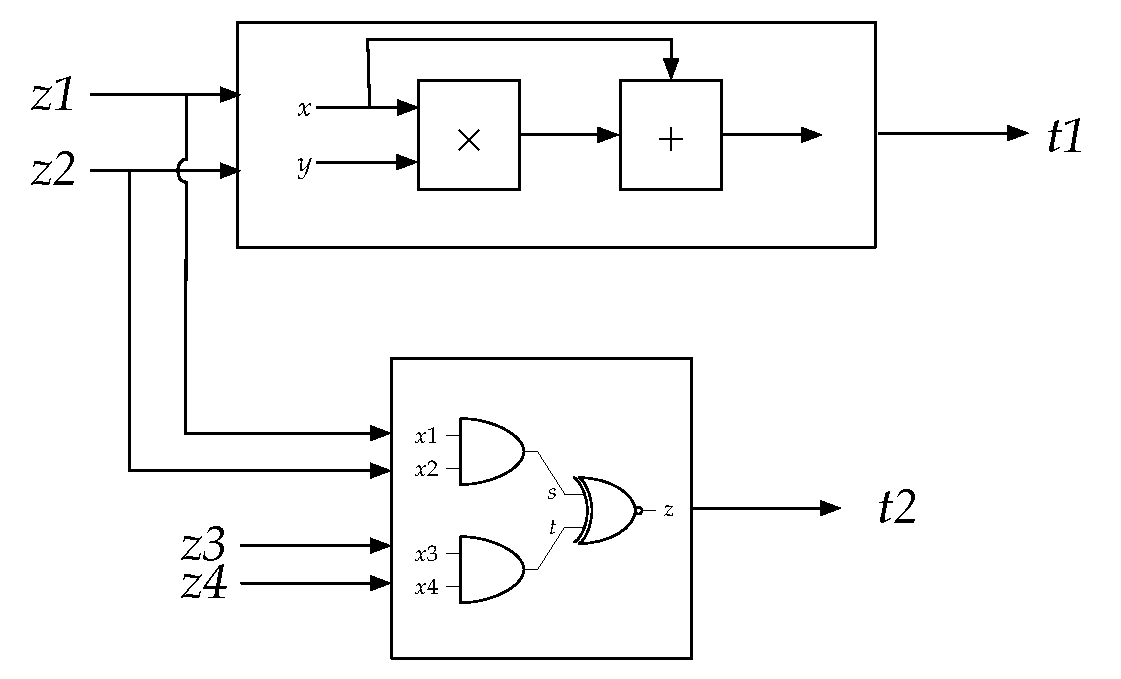
\includegraphics[width=0.9\textwidth]{images/muladdcomblogic}
\end{center}
\caption{Combination of figures \ref{fig:combinational1} and \ref{fig:muladd}.} \label{fig:combinational3}
\end{figure}


% Polymorphism
\subsubsection{Polymorphism}
The specification of a piece of digital logic is sometimes generic enough to be used in multiple ways.
The addition operation can for instance be used to add numbers regardless of their bit-representation, at least a language perspective.
When the addition operation is translated to \gls{vhdl}, a proper adder may be chosen. 
Due to the type system, we know the type of the numbers which are to be added, and as such a specific adder can be chosen.
Polymorphism makes it possible to specify and \textit{reuse} such specifications.
As an example of how code reuse is useful, consider the following code snippet, which represents the circuit of figure \ref{fig:polymorphic}.

\begin{texexptitled}[text only]{A polymorphic specification}{code:polymorphic}\begin{hscode}\SaveRestoreHook
\column{B}{@{}>{\hspre}l<{\hspost}@{}}%
\column{3}{@{}>{\hspre}l<{\hspost}@{}}%
\column{5}{@{}>{\hspre}l<{\hspost}@{}}%
\column{13}{@{}>{\hspre}l<{\hspost}@{}}%
\column{E}{@{}>{\hspre}l<{\hspost}@{}}%
\>[3]{}\Varid{commonCode}\;\Varid{f}\;\Varid{g}\;\Varid{h}\;\Varid{x}\;\Varid{y}\mathrel{=}\Varid{z3}{}\<[E]%
\\
\>[3]{}\hsindent{2}{}\<[5]%
\>[5]{}\mathbf{where}\;{}\<[13]%
\>[13]{}\Varid{z1}\mathrel{=}\Varid{f}\;\Varid{x}\;\Varid{y}{}\<[E]%
\\
\>[13]{}\Varid{z2}\mathrel{=}\Varid{g}\;\Varid{z1}{}\<[E]%
\\
\>[13]{}\Varid{z3}\mathrel{=}\Varid{h}\;\Varid{z2}\;\Varid{y}{}\<[E]%
\ColumnHook
\end{hscode}\resethooks
\end{texexptitled}

\begin{figure}[H]
\begin{center}
\centering
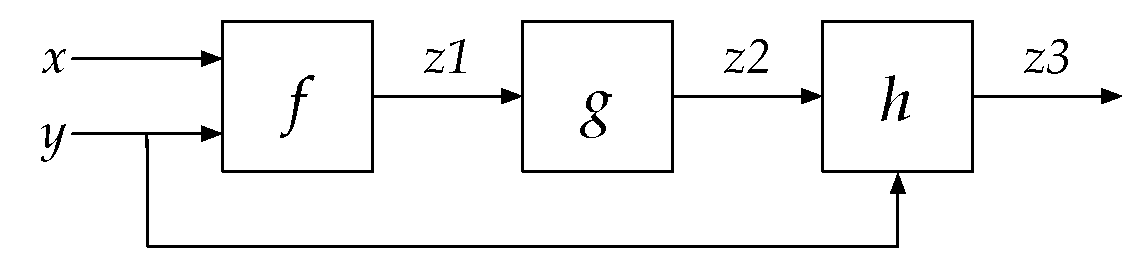
\includegraphics[width=0.8\textwidth]{images/polymorphic}
\end{center}
\caption{A polymorphic circuit, as specified by code snippet \ref{code:polymorphic}} \label{fig:polymorphic}
\end{figure}

The code of snippet \ref{code:polymorphic} only specifies in what way the functions \ensuremath{\Varid{f}},\ensuremath{\Varid{g}} and \ensuremath{\Varid{h}} interact with each other.
As the definition of \ensuremath{\Varid{commonCode}} uses the functions \ensuremath{\Varid{f}},\ensuremath{\Varid{g}} and \ensuremath{\Varid{h}} as arguments, the \ensuremath{\Varid{commonCode}} function needs to be applied to three different functions before the specification can be applied to bit-representable values.
For instance, we can use \ensuremath{\Varid{commonCode}} as 
\begin{changemargin}{1cm}{0cm}
\begin{expansionno}{text only}
\ensuremath{\Varid{specificCodeA}\mathrel{=}\Varid{commonCode}\;(\mathbin{+})\;\Varid{id}\;(\mathbin{+})}
\end{expansionno}
\end{changemargin}
or as 
\begin{changemargin}{1cm}{0cm}
\begin{expansionno}{text only}
\ensuremath{\Varid{specificCodeB}\mathrel{=}\Varid{commonCode}\;(\mathbin{*})\;\Varid{shiftL}\;(\mathbin{+})}
\end{expansionno}
\end{changemargin}
, depending on the intented usage of the \ensuremath{\Varid{commonCode}} pattern.

Both of those specifications are correct.
However, not every combination of functions leads to a correct specification.
When we use \ensuremath{\Varid{commonCode}} as in 
\begin{changemargin}{1cm}{0cm}
\begin{expansionno}{text only}
\ensuremath{\Varid{incorrectCode}\mathrel{=}\Varid{commonCode}\;(\mathbin{+})\;(\mathbin{+})\;(\mathbin{+})}
\end{expansionno}
\end{changemargin}
, then the second \ensuremath{(\mathbin{+})} function does not match with the function type which \ensuremath{\Varid{g}} is expected to have.
This is because there exists a \textit{relation} between the functions \ensuremath{\Varid{f}}, \ensuremath{\Varid{g}} and \ensuremath{\Varid{h}} within the context of the function \ensuremath{\Varid{commonCode}}.
We use \textit{type variables} to reason about these relationships.
Like value variables, type variables are referentially transparent.
For instance, the sub-expressions of \ensuremath{\Varid{commonCode}} have the following types:
\begin{changemargin}{1cm}{0cm}
\begin{expansionno}{text only}
\begin{hscode}\SaveRestoreHook
\column{B}{@{}>{\hspre}l<{\hspost}@{}}%
\column{5}{@{}>{\hspre}l<{\hspost}@{}}%
\column{E}{@{}>{\hspre}l<{\hspost}@{}}%
\>[B]{}\Varid{f}{}\<[5]%
\>[5]{}\mathbin{::}\Varid{a}\to \Varid{b}\to \Varid{c}{}\<[E]%
\\
\>[B]{}\Varid{g}{}\<[5]%
\>[5]{}\mathbin{::}\Varid{c}\to \Varid{d}{}\<[E]%
\\
\>[B]{}\Varid{h}{}\<[5]%
\>[5]{}\mathbin{::}\Varid{d}\to \Varid{b}\to \Varid{e}{}\<[E]%
\\
\>[B]{}\Varid{z1}{}\<[5]%
\>[5]{}\mathbin{::}\Varid{c}{}\<[E]%
\\
\>[B]{}\Varid{z2}{}\<[5]%
\>[5]{}\mathbin{::}\Varid{d}{}\<[E]%
\\
\>[B]{}\Varid{z3}{}\<[5]%
\>[5]{}\mathbin{::}\Varid{e}{}\<[E]%
\ColumnHook
\end{hscode}\resethooks
\end{expansionno}
\end{changemargin}
The type variables express the relation between the types of the expressions used in \ensuremath{\Varid{commonCode}}.
As \ensuremath{\Varid{f}} provides the input to \ensuremath{\Varid{g}}, the type of the input to \ensuremath{\Varid{g}} is necessarily the same as the type of the output of \ensuremath{\Varid{f}}.
The types of the remaining expressions are similarly limited.

Polymorphic types have a limitation however.
Since polymorphic types represent a range of possible representations, we can not generate hardware from a polymorphic description.
Thus, the final compilation must have fully determined types.

%%%%
% Combinational Logic and Time
%%%%
\subsection{Combinational Logic and Time}
In reality it takes time for outputs of combinational logic to become stable after a change occurs at the inputs of the circuit.
However, in synchronous hardware design this delay cannot be observed.
When the input changes, the output changes in the same timeframe.
Even though verification of time-dependent behaviour is not useful for combinational logic, the distinction between combinational logic and sequential logic still has to be made.
For this reason, the relation between inputs and outputs in combinational logic is made explicit by naming the moments at which values should exist.
To do so, we introduce time variables.
We use variables since we do not yet know at which specific time the input changes, but we would like to reason about the relation between input and output in terms of time.

Through the type system, we already have access to type information about the values used in expressions.
From the \ensuremath{\Varid{combLogic}} definition we know that \ensuremath{\Varid{combLogic}} is a function.
However, we also know that \ensuremath{\Varid{x1}} to \ensuremath{\Varid{x4}} are values with type \ensuremath{\Conid{Bit}}.
Similarly, we know the output value is of type \ensuremath{\Conid{Bit}} as well.
If we assume the output changes at moment \ensuremath{\Varid{t}}, then the input values must have stabilised at moment \ensuremath{\Varid{t}} as well.
We represent that as part of the type ascription by annotating each datatype with the same time variable as follows:
\begin{changemargin}{1cm}{0cm}
\begin{expansionno}{text only}
\ensuremath{\Varid{combLogic}\mathbin{::}\Conid{Bit}\langle\Varid{t}\rangle\to \Conid{Bit}\langle\Varid{t}\rangle\to \Conid{Bit}\langle\Varid{t}\rangle\to \Conid{Bit}\langle\Varid{t}\rangle\to \Conid{Bit}\langle\Varid{t}\rangle}
\ensuremath{\Varid{combLogic}\;\Varid{x1}\;\Varid{x2}\;\Varid{x3}\;\Varid{x4}\mathrel{=}\mathbin{...}}
\end{expansionno}
\end{changemargin}

In the above example we have defined every value to be available at the same moment in time, as is expected of combinational logic in synchronous hardware designs.
In synchronous hardware design we can always combine as much combinational logic as we wish, without having any impact on its \textit{modelled} time-dependent behaviour.
By adding more combinational logic, the time-dependent behaviour of the circuit stays the same, even though in reality, the performance suffers.

%%%%%%%%%%%%%%%%%%
%
% Sequential Logic
%
%%%%%%%%%%%%%%%%%%
\section{Specification of Sequential Logic}
Unlike combinational logic, sequential logic can not be described directly by pure functions.
Pure functions relate the output directly in terms of the input(s).
In sequential logic however, the current output does not solely depend on current input(s), but also on past input(s).
In this section we discuss how sequential logic is currently specified in \gls{clash}.
Next, we introduce how we can use time variables to specify time-dependent behaviour.
To do so, we focus on individual memory elements before defining a pipelined circuit.
Following pipelining, we discuss type (re)construction of compositions.
Finally, we discuss bounded sequences.

So far we have only shown how \gls{clash} represents combinational logic using pure functions.
Since pure functions are side-effect free, pure functions alone cannot be used to recall information from the past.
As a result, sequential logic in \gls{clash} is first defined as a pure function with a \textit{specific} type of type.
The pure function is then transformed into a component through a primitive function called \ensuremath{\Varid{lift}}, a process which is explained in greater detail later.
In this specific type of pure function, only combinational logic is defined, while sequential logic is solely represented via its inputs and outputs.

Code snippet \ref{code:sequentiallogic} shows the pattern which must be used to specify sequential logic.
As before, there is a immediate relationship between the code presented in code snippet \ref{code:sequentiallogic} and the circuit of figure \ref{fig:sequential}.

\begin{texexptitled}[text only]{Sequential logic in \gls{clash}}{code:sequentiallogic}\begin{hscode}\SaveRestoreHook
\column{B}{@{}>{\hspre}l<{\hspost}@{}}%
\column{3}{@{}>{\hspre}l<{\hspost}@{}}%
\column{5}{@{}>{\hspre}l<{\hspost}@{}}%
\column{13}{@{}>{\hspre}l<{\hspost}@{}}%
\column{19}{@{}>{\hspre}l<{\hspost}@{}}%
\column{E}{@{}>{\hspre}l<{\hspost}@{}}%
\>[3]{}\Varid{sequential}\mathbin{::}\Conid{State}\;\Varid{a}\to \Varid{b}\to (\Conid{State}\;\Varid{a},\Varid{c}){}\<[E]%
\\
\>[3]{}\Varid{sequential}\;(\Conid{State}\;\Varid{s})\;\Varid{x}\mathrel{=}(\Conid{State}\;\Varid{s'},\Varid{out}){}\<[E]%
\\
\>[3]{}\hsindent{2}{}\<[5]%
\>[5]{}\mathbf{where}\;{}\<[13]%
\>[13]{}\Varid{s'}{}\<[19]%
\>[19]{}\mathrel{=}\mathbin{...}{}\<[E]%
\\
\>[13]{}\Varid{out}{}\<[19]%
\>[19]{}\mathrel{=}\mathbin{...}{}\<[E]%
\ColumnHook
\end{hscode}\resethooks
\end{texexptitled}

The definition of \ensuremath{\Varid{sequential}} shows the type of the pure function used to describe sequential logic.
The first argument named \ensuremath{\Varid{s}} represents the input value from sequential logic of the \textit{current clockcycle}.
To distinguish between the inputs of sequential logic, and inputs of the component itself, the \ensuremath{\Conid{State}} keyword is used. 
The \ensuremath{\Conid{State}} keyword is \gls{clash} specific, and only has meaning in this specific type of function type.
In Haskell, \ensuremath{\Conid{State}} is a normal type constructor, whereas in \gls{clash} it is a reserved word.
To supply sequential logic with external input the second argument, named \ensuremath{\Varid{x}}, is used.
Using the variables \ensuremath{\Varid{s}} and \ensuremath{\Varid{x}}, the output \ensuremath{\Varid{out}} and the value of \ensuremath{\Varid{s}} in the \textit{next} clockcycle can be determined.
As a result, the input and output are synchronised to a clock, even though the specification of sequential logic does not specify the clock signal directly.
Instead, the relation between the input and the output of sequential logic is defined within the context of a single clock cycle.

\begin{figure}[H]
\begin{center}
\centering
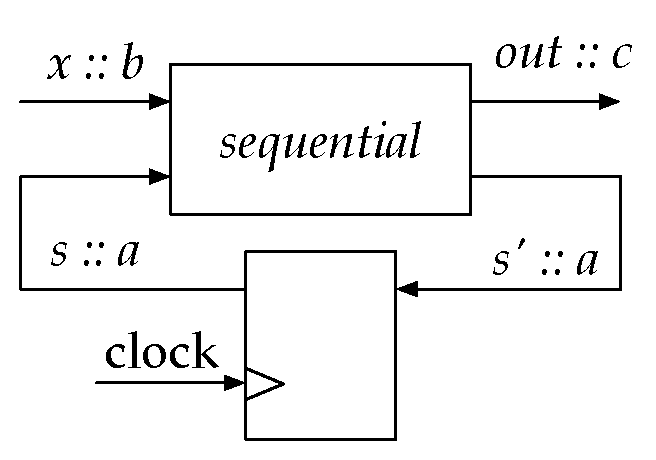
\includegraphics[width=0.5\textwidth]{images/sequential}
\end{center}
\caption{Sequential logic.} \label{fig:sequential}
\end{figure}

%%%%
% Individual Memory Elements
%%%%
\subsection{Individual Memory Elements}
Although the definition of sequential logic in \gls{clash} is flexible enough to specify feedback, we focus on a more simplified example first.
Code snippet \ref{code:singlemem} shows how a single memory element can be defined in \gls{clash}.
Like before, there exists an immediate relationship between the code and the circuit it represents.
In this example, a single type variable is enough to fully describe its behaviour.

\begin{texexptitled}[text only]{A single memory element in \gls{clash}}{code:singlemem}\begin{hscode}\SaveRestoreHook
\column{B}{@{}>{\hspre}l<{\hspost}@{}}%
\column{3}{@{}>{\hspre}l<{\hspost}@{}}%
\column{5}{@{}>{\hspre}l<{\hspost}@{}}%
\column{13}{@{}>{\hspre}l<{\hspost}@{}}%
\column{19}{@{}>{\hspre}l<{\hspost}@{}}%
\column{E}{@{}>{\hspre}l<{\hspost}@{}}%
\>[3]{}\Varid{singleMem}\mathbin{::}(\Conid{State}\;\Varid{a})\to \Varid{a}\to (\Conid{State}\;\Varid{a},\Varid{a}){}\<[E]%
\\
\>[3]{}\Varid{singleMem}\;(\Conid{State}\;\Varid{s})\;\Varid{x}\mathrel{=}(\Conid{State}\;\Varid{s'},\Varid{out}){}\<[E]%
\\
\>[3]{}\hsindent{2}{}\<[5]%
\>[5]{}\mathbf{where}\;{}\<[13]%
\>[13]{}\Varid{s'}{}\<[19]%
\>[19]{}\mathrel{=}\Varid{x}{}\<[E]%
\\
\>[13]{}\Varid{out}{}\<[19]%
\>[19]{}\mathrel{=}\Varid{s}{}\<[E]%
\ColumnHook
\end{hscode}\resethooks
\end{texexptitled}

%\begin{figure}[H]
%\begin{center}
%\centering
%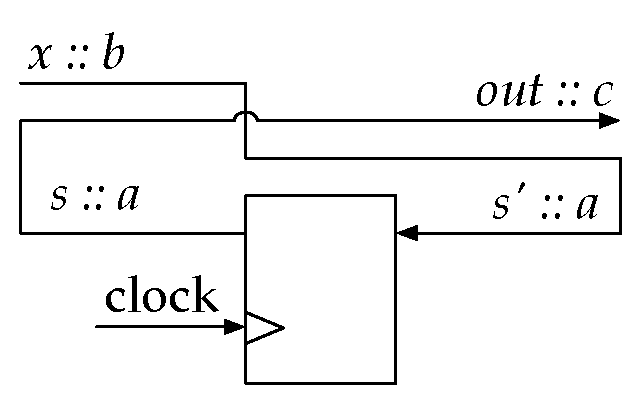
\includegraphics[width=0.5\textwidth]{images/singlememory}
%\end{center}
%\caption{A single memory element in \gls{clash}.} \label{fig:singlememory}
%\end{figure}

The same behaviour is modelled more concisely in our type system.
As shown, the definition of \ensuremath{\Varid{singleMem}} delays the input \ensuremath{\Varid{x}} with one cycle of the clock.
Delaying a value with one clockcycle implies some form of transformation in the time domain.
Instead of specifying the input and output of sequential logic separately, we directly encode this transformation in the type of the function.
As shown by code snippet \ref{code:singlememvar}, the intent of the specification which uses time variables is clear from the type of the function alone.
The input exists at time \ensuremath{\Varid{t}}, and the output exists one cycle later, at \ensuremath{\Varid{t}\mathbin{+}\mathrm{1}}.

\begin{texexptitled}[text only]{A single memory element defined using a time variable.}{code:singlememvar}\begin{hscode}\SaveRestoreHook
\column{B}{@{}>{\hspre}l<{\hspost}@{}}%
\column{3}{@{}>{\hspre}l<{\hspost}@{}}%
\column{E}{@{}>{\hspre}l<{\hspost}@{}}%
\>[3]{}\Varid{singleMem'}\mathbin{::}\Varid{a}\langle\Varid{t}\rangle\to \Varid{a}\langle\Varid{t}\mathbin{+}\mathrm{1}\rangle{}\<[E]%
\\
\>[3]{}\Varid{singleMem'}\;\Varid{x}\mathrel{=}\Varid{x}{}\<[E]%
\ColumnHook
\end{hscode}\resethooks
\end{texexptitled}

Instead of introducing temporal transformations at the term level, we introduce such transformations as part of the type. 
A memory element behaves as the identity function in the value domain, and as a linear transformation in the time-domain.
Variables on the term level are referentially transparent; they can be replaced by the same value throughout the expression without changing the behaviour of the function.
This is true when applying a positive shift to the time-domain of a value as well.
When a value exists at some point in time \ensuremath{\Varid{t}}, it can always be stored to be available at \ensuremath{\Varid{t}\mathbin{+}\Varid{a}}, where \ensuremath{\Varid{a}} is any natural number.
Specifying the time-dependent behaviour as part of the function type leads to a clean separation between \textit{what} ought to be done by a function, and \textit{when} it ought to be done.

Memory elements defined in this way have limitations however.
Memory elements which have some conditional behaviour cannot be expressed solely by transformations in the time domain.
To describe such memory elements, either a language primitive needs to be added, or the needed type of memory element should be detected from contextual information during translation to \gls{vhdl} or during hardware synthesis.

Similarly to \gls{clash}, the clock is not explicitly defined.
Even so, a relation between the time variable \ensuremath{\Varid{t}}, the expression \ensuremath{\Varid{t}\mathbin{+}\mathrm{1}} and the clock exists, as shown by figure \ref{fig:clock}.

\begin{figure}[H]
\begin{center}
\centering
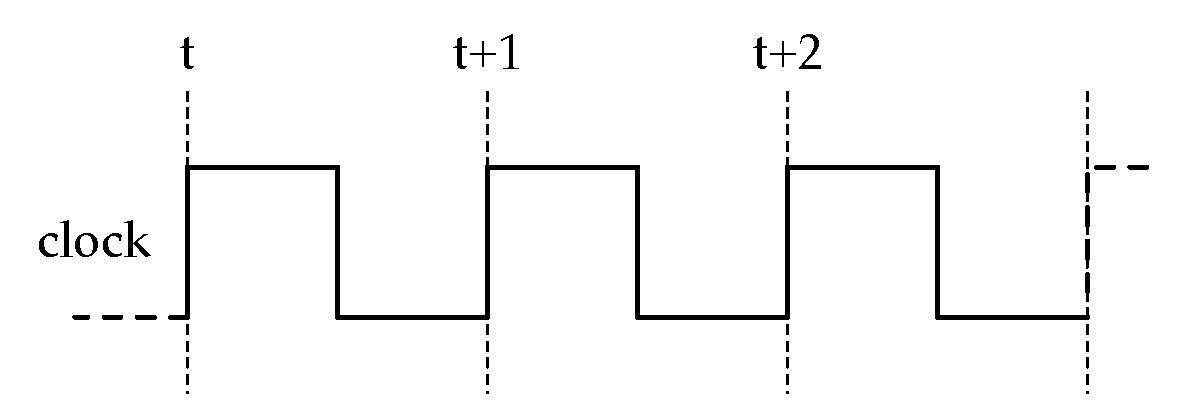
\includegraphics[width=0.6\textwidth]{images/clock}
\end{center}
\caption{Relation between the clock and time variables} \label{fig:clock}
\end{figure}

Time variables represent specific moments in ``real'' time.
However, time is discrete and as such we cannot distinguish between two moments in time which occur between $t$ and $t + 1$.
In synchronous logic, a period of time needs to pass in order for signals to stabilise.
The moment in time \ensuremath{\Varid{t}} represents the first moment when its input is stable.
The time expression \ensuremath{\Varid{t}\mathbin{+}\mathrm{1}} as part of the output defines when this output will stabilise, in relation to its input.

Similarly to the definition of \ensuremath{\Varid{singleMem}}, we can define two memory elements by changing the offset, as shown by code snippet \ref{code:doublememvar}.
\begin{texexptitled}[text only]{Two memory elements defined using a time variable.}{code:doublememvar}\begin{hscode}\SaveRestoreHook
\column{B}{@{}>{\hspre}l<{\hspost}@{}}%
\column{3}{@{}>{\hspre}l<{\hspost}@{}}%
\column{E}{@{}>{\hspre}l<{\hspost}@{}}%
\>[3]{}\Varid{doubleMem}\mathbin{::}\Varid{a}\langle\Varid{t}\rangle\to \Varid{a}\langle\Varid{t}\mathbin{+}\mathrm{2}\rangle{}\<[E]%
\\
\>[3]{}\Varid{doubleMem}\;\Varid{x}\mathrel{=}\Varid{x}{}\<[E]%
\ColumnHook
\end{hscode}\resethooks
\end{texexptitled}

We compose \ensuremath{\Varid{doubleMem}} with \ensuremath{\Varid{singleMem}} to create \ensuremath{\Varid{tripleMem}}.
The type system can infer the correct type of the composition.
As a result, the type of 
\begin{changemargin}{1cm}{0cm}
\begin{expansionno}{text only}
\ensuremath{\Varid{tripleMem}\mathrel{=}\Varid{doubleMem}\mathbin{\circ}\Varid{singleMem}}
\end{expansionno}
\end{changemargin}
is inferred to be \ensuremath{\Varid{a}\langle\Varid{t}\rangle\to \Varid{a}\langle\Varid{t}\mathbin{+}\mathrm{3}\rangle}.

Even though the hardware specifications so far have always used the same time variable, time variables are not shared between specifications.
Time variables only exist within the scope of the specification where they are introduced.
As a result, the time variable used in \ensuremath{\Varid{singleMem}} is different from the time variable used in \ensuremath{\Varid{doubleMem}}, even though they use the same identifier.

%%%%
% Pipelining
%%%%
\subsection{Pipelining}
The definition of a single memory element is straightforward in \gls{clash} as is, so it may be hard to see exactly how adding time-dependent behaviour can be advantageous based on the examples from the previous section.
To show how adding time-dependent behaviour to the type system can lead to more concise specifications, consider the following circuit.

\begin{figure}[H]
\begin{center}
\centering
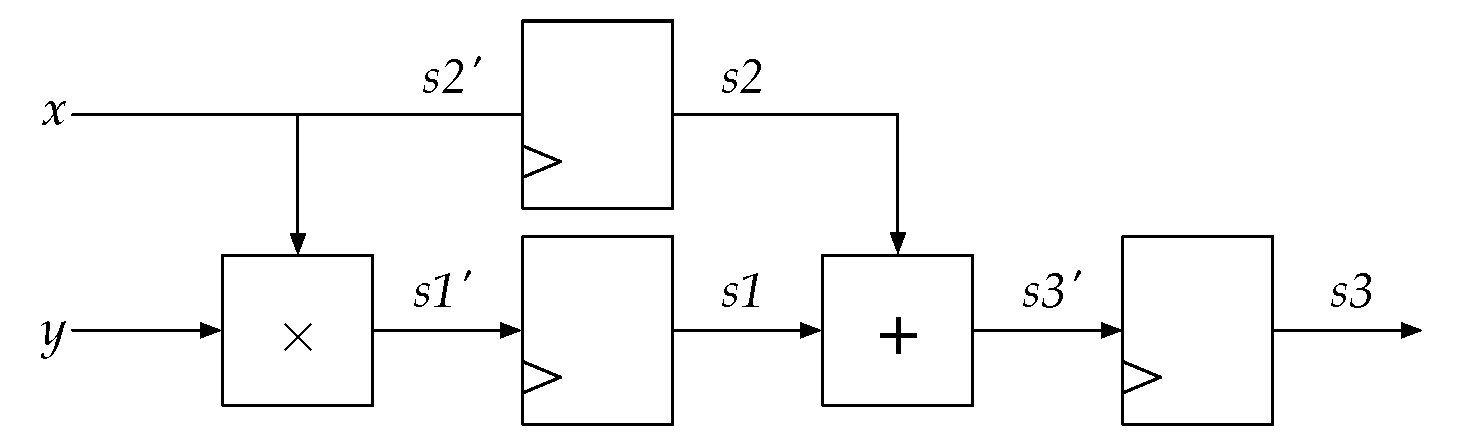
\includegraphics[width=\textwidth]{images/pipeline}
\end{center}
\caption{A pipelined circuit} \label{fig:pipeline}
\end{figure}

\gls{clash} is able to represent the circuit as a single pure function as shown by code snippet \ref{code:pipeline}.
The \ensuremath{\Conid{State}} keyword, together with the structure of the function type, allows us to transfer values between two clockcycles.
The variables \ensuremath{\Varid{s1},\Varid{s2},\Varid{s3}} represent the outputs from the registers, as opposed to the variables \ensuremath{\Varid{s1'},\Varid{s2'},\Varid{s3'}}, which represent the inputs of the registers.
This means that, given a definition of \ensuremath{\Varid{s1'}} at some clockcycle \ensuremath{\Varid{t}}, then \ensuremath{\Varid{s1}} has the same value as \ensuremath{\Varid{s1'}} at some clockcycle \ensuremath{\Varid{t}\mathbin{+}\mathrm{1}}.
This relation is straightforward, but when many registers are added, the function definitions soon become complex. 

\begin{texexptitled}[text only]{Definition of a pipeline in \gls{clash}.}{code:pipeline}\begin{hscode}\SaveRestoreHook
\column{B}{@{}>{\hspre}l<{\hspost}@{}}%
\column{3}{@{}>{\hspre}l<{\hspost}@{}}%
\column{6}{@{}>{\hspre}l<{\hspost}@{}}%
\column{13}{@{}>{\hspre}l<{\hspost}@{}}%
\column{38}{@{}>{\hspre}l<{\hspost}@{}}%
\column{E}{@{}>{\hspre}l<{\hspost}@{}}%
\>[3]{}\Varid{pipeline}\mathbin{::}\Conid{State}\;(\Conid{Int},\Conid{Int},\Conid{Int})\to (\Conid{Int},\Conid{Int})\to (\Conid{State}\;(\Conid{Int},\Conid{Int},\Conid{Int}),\Conid{Int}){}\<[E]%
\\
\>[3]{}\Varid{pipeline}\;(\Conid{State}\;(\Varid{s1},\Varid{s2},\Varid{s3}))\;(\Varid{x},\Varid{y}){}\<[38]%
\>[38]{}\mathrel{=}(\Conid{State}\;(\Varid{s1'},\Varid{s2'},\Varid{s3'}),\Varid{s3}){}\<[E]%
\\
\>[3]{}\hsindent{3}{}\<[6]%
\>[6]{}\mathbf{where}\;{}\<[13]%
\>[13]{}\Varid{s1'}\mathrel{=}\Varid{x}\mathbin{*}\Varid{y}{}\<[E]%
\\
\>[13]{}\Varid{s2'}\mathrel{=}\Varid{x}{}\<[E]%
\\
\>[13]{}\Varid{s3'}\mathrel{=}\Varid{s1}\mathbin{+}\Varid{s2}{}\<[E]%
\ColumnHook
\end{hscode}\resethooks
\end{texexptitled}

Fortunately, \gls{clash} makes it possible to create better structural descriptions by lifting pure functions such as \ensuremath{\Varid{pipeline}} to the component level.
The component level, which is based on arrows\cite{hudak2003arrows}, allows us to interpret the pure function \ensuremath{\Varid{pipeline}} as an impure function with embedded state.
Although a complete introduction to component-based programming in \gls{clash} is out of the scope of this thesis, we can show the advantages and disadvantages of the approach.
Code snippet \ref{code:pipelinec} shows the structural representation of the circuit from figure \ref{fig:pipeline}.
The \ensuremath{\Varid{lift}} function, ``lifts'' a pure function to the component level.
Unfortunately, to do so, the \textit{initial} content of the memory element has to be specified when using the lifting function.
As shown by the schematic of figure \ref{fig:pipeline}, no initial values are needed for this circuit to function properly.
Without initial values, there is a latency of two clockcycles, before the circuit produces a meaningful result.

\begin{texexptitled}[text only]{Definition of a pipeline in \gls{clash} using arrows.}{code:pipelinec}\begin{hscode}\SaveRestoreHook
\column{B}{@{}>{\hspre}l<{\hspost}@{}}%
\column{3}{@{}>{\hspre}l<{\hspost}@{}}%
\column{5}{@{}>{\hspre}l<{\hspost}@{}}%
\column{22}{@{}>{\hspre}l<{\hspost}@{}}%
\column{30}{@{}>{\hspre}l<{\hspost}@{}}%
\column{E}{@{}>{\hspre}l<{\hspost}@{}}%
\>[3]{}\Varid{pipelineC}\mathrel{=}\textbf{proc}\;(\Varid{x},\Varid{y})\to \mathbf{do}{}\<[E]%
\\
\>[3]{}\hsindent{2}{}\<[5]%
\>[5]{}\Varid{s1}\leftarrow\Varid{singleMem}{}\<[22]%
\>[22]{}\mathbin{`\Varid{lift}`}{}\<[30]%
\>[30]{}\mathrm{0}\prec\Varid{x}\mathbin{+}\Varid{y}{}\<[E]%
\\
\>[3]{}\hsindent{2}{}\<[5]%
\>[5]{}\Varid{s2}\leftarrow\Varid{singleMem}{}\<[22]%
\>[22]{}\mathbin{`\Varid{lift}`}{}\<[30]%
\>[30]{}\mathrm{0}\prec\Varid{x}{}\<[E]%
\\
\>[3]{}\hsindent{2}{}\<[5]%
\>[5]{}\Varid{s3}\leftarrow\Varid{singleMem}{}\<[22]%
\>[22]{}\mathbin{`\Varid{lift}`}{}\<[30]%
\>[30]{}\mathrm{0}\prec\Varid{s1}\mathbin{+}\Varid{s2}{}\<[E]%
\\
\>[3]{}\hsindent{2}{}\<[5]%
\>[5]{}\textbf{returnA}\prec\Varid{s3}{}\<[E]%
\ColumnHook
\end{hscode}\resethooks
\end{texexptitled}

Initial values have to be supplied regardless of the method used to create sequential logic.
Even the pure function \ensuremath{\Varid{pipeline}}, has to be lifted to the component level, before translating it to \gls{vhdl}.
As shown by \ensuremath{\Varid{pipelineC}}, the component level has a different syntax when compared to the functions shown earlier.
Usage of the language is more difficult as a result, due to the added syntax to describe interactions between components and the complexity of the underlying arrows model.

When we compare this with the code of snippet \ref{code:pipeline'}, we see that specification using time variables at the type level is a more concise way to specify time-dependent behaviour.

\begin{texexptitled}[text only]{Definition of a pipeline using time variables.}{code:pipeline'}\begin{hscode}\SaveRestoreHook
\column{B}{@{}>{\hspre}l<{\hspost}@{}}%
\column{3}{@{}>{\hspre}l<{\hspost}@{}}%
\column{E}{@{}>{\hspre}l<{\hspost}@{}}%
\>[3]{}\Varid{pipeline'}\mathbin{::}\Conid{Int}\langle\Varid{t}\rangle\to \Conid{Int}\langle\Varid{t}\rangle\to \Conid{Int}\langle\Varid{t}\mathbin{+}\mathrm{2}\rangle{}\<[E]%
\\
\>[3]{}\Varid{pipeline'}\;\Varid{x}\;\Varid{y}\mathrel{=}(\Varid{x}\mathbin{*}\Varid{y})\mathbin{+}\Varid{x}{}\<[E]%
\ColumnHook
\end{hscode}\resethooks
\end{texexptitled}

Even though the presentation is fairly concise, the definition of \ensuremath{\Varid{pipeline'}} is not equal to \gls{clash}'s definition.
Given the definition of \ensuremath{\Varid{pipeline'}}, the compiler cannot determine where \textit{exactly} memory elements ought to be inserted.
Based on the supplied function type, we know that the entire expression \ensuremath{(\Varid{x}\mathbin{*}\Varid{y})\mathbin{+}\Varid{x}} has type \ensuremath{\Conid{Int}\langle\Varid{t}\mathbin{+}\mathrm{2}\rangle}, while \ensuremath{\Varid{x}} and \ensuremath{\Varid{y}} have type \ensuremath{\Conid{Int}\langle\Varid{t}\rangle}.
We know two memory elements are needed in order to make the transformation from \ensuremath{\Varid{t}} to \ensuremath{\Varid{t}\mathbin{+}\mathrm{2}} possible, but we cannot determine where these elements ought to be inserted.
Using retiming\cite{leiserson1981optimizing}, the optimal placing of memory elements can be determined.
However, that still does not give the ability to define the circuit of figure \ref{fig:pipeline}.

To do so, individual functions representing memory elements can be added.
Since our language does not support function overloading, nor the mechanisms to use a function twice, two functions need to be defined in order to fully define the circuit of figure \ref{fig:pipeline}.
If a single \ensuremath{\Varid{delay}} function is added, such as in \ensuremath{\Varid{pipeline''}} below, the time-dependent behaviour of the circuit is defined more precisely.

\begin{texexptitled}[text only]{Definition of a pipeline using time variables and a delay.}{code:pipeline''}\begin{hscode}\SaveRestoreHook
\column{B}{@{}>{\hspre}l<{\hspost}@{}}%
\column{3}{@{}>{\hspre}l<{\hspost}@{}}%
\column{E}{@{}>{\hspre}l<{\hspost}@{}}%
\>[3]{}\Varid{pipeline''}\mathbin{::}\Conid{Int}\langle\Varid{t}\rangle\to \Conid{Int}\langle\Varid{t}\rangle\to \Conid{Int}\langle\Varid{t}\mathbin{+}\mathrm{2}\rangle{}\<[E]%
\\
\>[3]{}\Varid{pipeline''}\;\Varid{x}\;\Varid{y}\mathrel{=}((\Varid{delay}\;\Varid{y})\mathbin{*}\Varid{x})\mathbin{+}\Varid{x}{}\<[E]%
\\[\blanklineskip]%
\>[3]{}\Varid{delay}\mathbin{::}\Conid{Int}\langle\Varid{t}\rangle\to \Conid{Int}\langle\Varid{t}\mathbin{+}\mathrm{1}\rangle{}\<[E]%
\\
\>[3]{}\Varid{delay}\;\Varid{x}\mathrel{=}\Varid{x}{}\<[E]%
\ColumnHook
\end{hscode}\resethooks
\end{texexptitled}

In \ensuremath{\Varid{pipeline''}}, \ensuremath{\Varid{y}} is explicitly delayed by one clock cycle before it is multiplied by \ensuremath{\Varid{x}}.
Then, assuming \ensuremath{(\mathbin{+})} represents an adder made with combinational logic, \ensuremath{\Varid{x}} must be delayed \textit{before} using it in the multiplication.
By expressing time as part of the type, in combination with retiming, we can choose the degree of specification.

The difficulty here, is to determine when the specification of some time-dependent behaviour should be subject to retiming.
This is not part of this thesis however, which is why we do not go into detail here.

\subsection{Type Reconstruction}
One of the most important aspects of our type system, is that variables are referentially transparant and only refer to single values.
This worked out for the examples \ensuremath{\Varid{pipeline'}} and \ensuremath{\Varid{singleMem'}} earlier.
In those examples, compositions were created from composing unary functions, or by composing combinational logic.
The type system can reconstruct the type of any valid composition of well-typed functions.
As an example, consider the \ensuremath{\Varid{delay}} and \ensuremath{\Varid{sel}} functions from code snippet \ref{code:possiblecomp}.

\begin{figure}[H]
\begin{center}
\centering
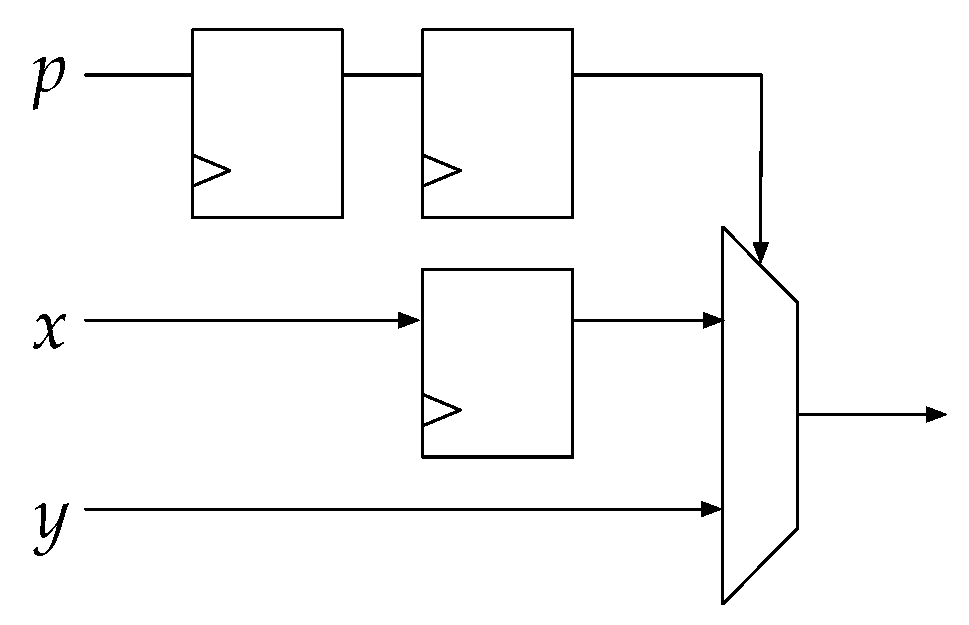
\includegraphics[width=0.6\textwidth]{images/sel}
\end{center}
\caption{Schematic representation of \ensuremath{\Varid{sel}}.} \label{fig:sel}
\end{figure}

\begin{texexptitled}[text only]{Delayed selection.}{code:possiblecomp}\begin{hscode}\SaveRestoreHook
\column{B}{@{}>{\hspre}l<{\hspost}@{}}%
\column{3}{@{}>{\hspre}l<{\hspost}@{}}%
\column{E}{@{}>{\hspre}l<{\hspost}@{}}%
\>[3]{}\Varid{sel}\mathbin{::}\Conid{Bool}\langle\Varid{t}\rangle\to \Conid{Int}\langle\Varid{t}\mathbin{+}\mathrm{1}\rangle\to \Conid{Int}\langle\Varid{t}\mathbin{+}\mathrm{2}\rangle\to \Conid{Int}\langle\Varid{t}\mathbin{+}\mathrm{2}\rangle{}\<[E]%
\\
\>[3]{}\Varid{sel}\;\Varid{p}\;\Varid{x}\;\Varid{y}\mathrel{=}\mathbf{if}\;\Varid{p}\;\mathbf{then}\;\Varid{x}\;\mathbf{else}\;\Varid{y}{}\<[E]%
\ColumnHook
\end{hscode}\resethooks
\begin{hscode}\SaveRestoreHook
\column{B}{@{}>{\hspre}l<{\hspost}@{}}%
\column{3}{@{}>{\hspre}l<{\hspost}@{}}%
\column{E}{@{}>{\hspre}l<{\hspost}@{}}%
\>[3]{}\Varid{delay}\mathbin{::}\Conid{Int}\langle\Varid{t}\rangle\to \Conid{Int}\langle\Varid{t}\mathbin{+}\mathrm{3}\rangle{}\<[E]%
\\
\>[3]{}\Varid{delay}\;\Varid{z}\mathrel{=}\Varid{z}{}\<[E]%
\ColumnHook
\end{hscode}\resethooks
\end{texexptitled}

As shown in the code, the value \ensuremath{\Varid{p}} needs to be delayed twice, in order to be used together with the value \ensuremath{\Varid{y}}.
The value \ensuremath{\Varid{x}} needs to be delayed once.
We combine the definition of \ensuremath{\Varid{sel}} with \ensuremath{\Varid{delay}} as follows:
\begin{changemargin}{1cm}{0cm}
\begin{expansionno}{text only}\begin{hscode}\SaveRestoreHook
\column{B}{@{}>{\hspre}l<{\hspost}@{}}%
\column{3}{@{}>{\hspre}l<{\hspost}@{}}%
\column{E}{@{}>{\hspre}l<{\hspost}@{}}%
\>[3]{}\Varid{comp}\;\Varid{w}\;\Varid{q}\mathrel{=}\Varid{sel}\;\Varid{q}\;\Varid{w}\;(\Varid{delay}\;\Varid{w}){}\<[E]%
\ColumnHook
\end{hscode}\resethooks
\end{expansionno}
\end{changemargin}

Through the application of \ensuremath{\Varid{sel}\;\Varid{q}} to \ensuremath{\Varid{w}}, \ensuremath{\Varid{w}} is equal to \ensuremath{\Varid{x}}.
Moreover, \ensuremath{\Varid{w}\mathrel{=}\Varid{z}} in \ensuremath{\Varid{delay}}, and \ensuremath{\Varid{z}\mathrel{=}\Varid{y}} through application of \ensuremath{\Varid{sel}}.
As a result, \ensuremath{\Varid{y}\mathrel{=}\Varid{x}}, which is seemingly impossible from the definition of \ensuremath{\Varid{sel}}.
The type of \ensuremath{\Varid{comp}} can reflect this however, by adding additional memory elements.
This is shown in figure \ref{fig:compseldelay}.

\begin{figure}[H]
\begin{center}
\centering
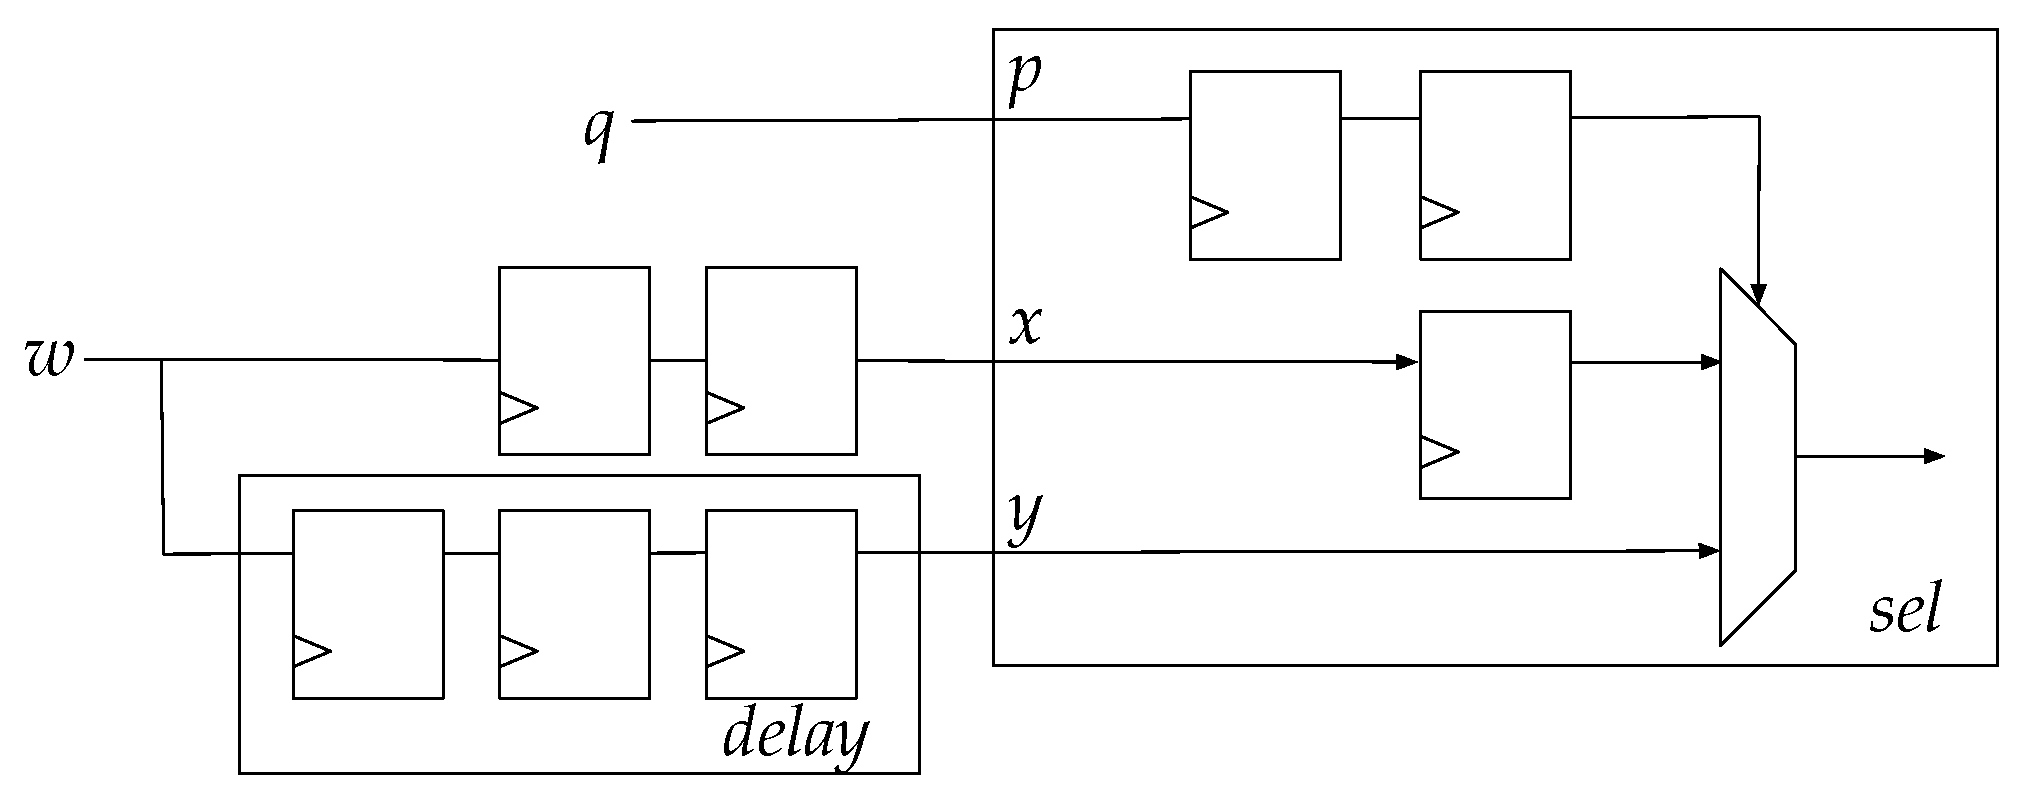
\includegraphics[width=0.9\textwidth]{images/compseldelay}
\end{center}
\caption{Schematic representation of \ensuremath{\Varid{sel}}.} \label{fig:compseldelay}
\end{figure}

As shown, two memory elements are added beyond those already available in \ensuremath{\Varid{delay}} and \ensuremath{\Varid{sel}}. 
This is done in order to equate \ensuremath{\Varid{w}} from \ensuremath{\Varid{comp}} with both \ensuremath{\Varid{x}} and \ensuremath{\Varid{y}} from \ensuremath{\Varid{sel}}.
As a result, the type of \ensuremath{\Varid{comp}} would be 
\begin{changemargin}{1cm}{0cm}
\begin{expansionno}{text only}\begin{hscode}\SaveRestoreHook
\column{B}{@{}>{\hspre}l<{\hspost}@{}}%
\column{3}{@{}>{\hspre}l<{\hspost}@{}}%
\column{E}{@{}>{\hspre}l<{\hspost}@{}}%
\>[3]{}\Varid{comp}\mathbin{::}\Conid{Int}\langle\Varid{t}\rangle\to \Conid{Bool}\langle\Varid{t}\mathbin{+}\mathrm{1}\rangle\to \Conid{Int}\langle\Varid{t}\mathbin{+}\mathrm{3}\rangle{}\<[E]%
\\
\>[3]{}\Varid{comp}\;\Varid{w}\;\Varid{q}\mathrel{=}\Varid{sel}\;\Varid{q}\;\Varid{w}\;(\Varid{delay}\;\Varid{w}){}\<[E]%
\ColumnHook
\end{hscode}\resethooks
\end{expansionno}
\end{changemargin}

There exist an odd side-effect of this automatic derivation however.
Due to how the typing rules are defined in the next chapter, functions can only be constructed where the arguments are ordered in time.
That is, a function type as \ensuremath{\Conid{Int}\langle\Varid{t}\rangle\to \Conid{Int}\langle\Varid{t}\mathbin{+}\mathrm{2}\rangle\to \Conid{Int}\langle\Varid{t}\mathbin{+}\mathrm{1}\rangle\to \Conid{Int}\langle\Varid{t}\mathbin{+}\mathrm{2}\rangle}, while seemingly valid, can not be constructed.
This side effect is most obvious when we derive the type of \ensuremath{\Varid{comp'}} below, in which the arguments \ensuremath{\Varid{w}} and \ensuremath{\Varid{q}} are flipped:
\begin{changemargin}{1cm}{0cm}
\begin{expansionno}{text only}\begin{hscode}\SaveRestoreHook
\column{B}{@{}>{\hspre}l<{\hspost}@{}}%
\column{3}{@{}>{\hspre}l<{\hspost}@{}}%
\column{E}{@{}>{\hspre}l<{\hspost}@{}}%
\>[3]{}\Varid{comp'}\mathbin{::}\Conid{Bool}\langle\Varid{t}\rangle\to \Conid{Int}\langle\Varid{t}\rangle\to \Conid{Int}\langle\Varid{t}\mathbin{+}\mathrm{3}\rangle{}\<[E]%
\\
\>[3]{}\Varid{comp'}\;\Varid{q}\;\Varid{w}\mathrel{=}\Varid{sel}\;\Varid{q}\;\Varid{w}\;(\Varid{delay}\;\Varid{w}){}\<[E]%
\ColumnHook
\end{hscode}\resethooks
\end{expansionno}
\end{changemargin}

Since arguments need to be ordered, the only way to derive a valid type from \ensuremath{\Varid{comp'}} is to add one additional register between the input to \ensuremath{\Varid{comp'}} and the input of \ensuremath{\Varid{sel}}. 

%%%%
% Sampling
%%%%
\subsection{Sequencing}
Using multiple input values which originate from the same wire is used frequently in synchronous hardware design, espcially in the area of \gls{dsp}.
We can not define such behaviour using only the syntax we have introduced earlier in this chapter, as explained in the previous section.
Consider the circuit of figure \ref{fig:sum2}, where two consecutive values are added.

\begin{figure}[H]
\begin{center}
\centering
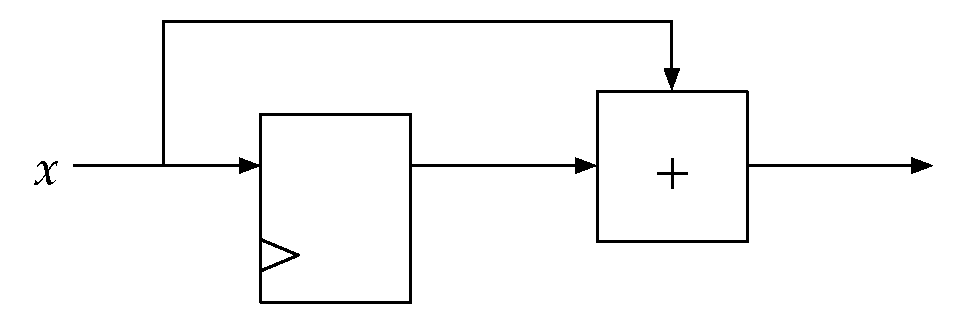
\includegraphics[width=0.6\textwidth]{images/sum2}
\end{center}
\caption{Adding two consecutive values.} \label{fig:sum2}
\end{figure}

In this schematic, \ensuremath{\Varid{x}} is not referentially transparant, as \ensuremath{\Varid{x}} refers to the wire, which represents multiple values. 
As shown in the previous section, this is not allowed in our descriptions, which makes it impossible to define this circuit directly through function abstraction and application.
Instead, we allow finite sequences of values.

\begin{texexptitled}[text only]{Summing two consecutive values.}{code:sum2}\begin{hscode}\SaveRestoreHook
\column{B}{@{}>{\hspre}l<{\hspost}@{}}%
\column{3}{@{}>{\hspre}l<{\hspost}@{}}%
\column{E}{@{}>{\hspre}l<{\hspost}@{}}%
\>[3]{}\Varid{sum2}\mathbin{::}\Conid{Int}\langle\Varid{t},\Varid{t}\mathbin{+}\mathrm{1}\rangle\to \Conid{Int}\langle\Varid{t}\mathbin{+}\mathrm{1}\rangle{}\<[E]%
\\
\>[3]{}\Varid{sum2}\langle\Varid{x1},\Varid{x2}\rangle\mathrel{=}\Varid{x1}\mathbin{+}\Varid{x2}{}\<[E]%
\ColumnHook
\end{hscode}\resethooks
\end{texexptitled}

In \ensuremath{\Varid{sum2}}, the first argument consists of two sequential values.
The type of first argument consists of two time variables, which match with the two identifiers \ensuremath{\Varid{x1}} and \ensuremath{\Varid{x2}}. 
By matching the identifiers with the time expressions, we show how \ensuremath{\Varid{x1}} relates to \ensuremath{\Varid{x2}}.
When this function is applied to another value, the correct \gls{vhdl} could, in principle at least, be generated.

The \ensuremath{\Varid{sum2}} function from above could similarly be represented as a binary function.
However, it can not be used in compositions in the same fashion as \ensuremath{\Varid{sum2}}.
As shown in the previous section, when \ensuremath{\Varid{sum2'}} is applied a single value twice, additional registers would be added to maintain referential transparency.

\begin{texexptitled}[text only]{Summing two consecutive values with a binary function.}{code:sum2'}\begin{hscode}\SaveRestoreHook
\column{B}{@{}>{\hspre}l<{\hspost}@{}}%
\column{3}{@{}>{\hspre}l<{\hspost}@{}}%
\column{E}{@{}>{\hspre}l<{\hspost}@{}}%
\>[3]{}\Varid{sum2'}\mathbin{::}\Conid{Int}\langle\Varid{t}\rangle\to \Conid{Int}\langle\Varid{t}\mathbin{+}\mathrm{1}\rangle\to \Conid{Int}\langle\Varid{t}\mathbin{+}\mathrm{1}\rangle{}\<[E]%
\\
\>[3]{}\Varid{sum2'}\;\Varid{x1}\;\Varid{x2}\mathrel{=}\Varid{x1}\mathbin{+}\Varid{x2}{}\<[E]%
\ColumnHook
\end{hscode}\resethooks
\end{texexptitled}

Sequences are really just a form of syntactic sugar.
In the next chapter, we show how functions of the form \ensuremath{\Varid{sum2'}} are converted to the equivalent of \ensuremath{\Varid{sum2}}.
Using a function with type
\begin{changemargin}{1cm}{0cm}
\begin{expansionno}{text only}
\ensuremath{\Varid{foo}\mathbin{::}\Varid{a}\langle\Varid{t}\rangle\to \Varid{a}\langle\Varid{t}\mathbin{+}\mathrm{1}\rangle\to \mathbin{...}\to \Varid{a}\langle\Varid{t}\mathbin{+}\Varid{n}\rangle\to \Varid{b}\langle\Varid{t}\mathbin{+}\Varid{n}\mathbin{+}\Varid{a}\rangle}
\end{expansionno}
\end{changemargin}
, we can derive the following structure including memory elements.

\begin{figure}[H]
\begin{center}
\centering
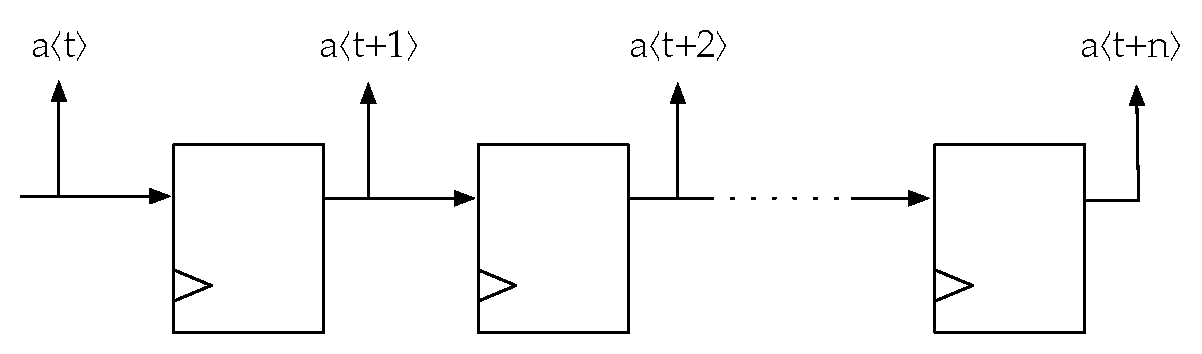
\includegraphics[width=0.8\textwidth]{images/sequence}
\end{center}
\caption{Structure generated by sequence usage.} \label{fig:sequence}
\end{figure}

The above structure only works for bit-representable values.
In a language where functions are not bit-representable, sequences can not be used for functions.

\section{Conclusion}
In this chapter we discussed the specification of time-dependent behaviour in a functional language using the type system.
One of the main advantages of the approach shown, is the fact that variables refer to \textit{individual values}.
This is different from most, if not all, existing functional hardware description languages.
In existing functional hardware description languages like Lava and \gls{forsyde}, streams are used.
In those languages, variables refer to streams of values.

In our approach, variables refer to individual values.
This is not without cost however, as variables need the ability to be moved through time.
Without the ability to be moved through time, variables which refer to individual values can not be used to describe time-dependent behaviour.
As a result from this ability, compositions of functions have a side effect.
By composing functions, additional memory elements can be added to the system.
This side-effect can be impredictable if one is not aware of its existence, which makes it less appealing to use in a hardware description language.

However, a great benefit of the expressing time-dependent behaviour in the way we showed, is that the definition of \textit{what} needs to be done is separated from \textit{when} it ought to be done.
This distinction makes it easier to reason about the time-dependent behaviour, without being concerned with what the function does, or vice versa.
By providing the ``when'' as part of the type, the time-dependent behaviour of compositions can be inferred, and checked by the system if the designer supplies the expected type.

%\subsection{Composing Sequences}
%%Before we compose various forms of sequences, it is important we point out that sequences exist \textit{solely} for specification purposes.
%%Since the time-dependent behaviour of sequences is known, we only use sequences to specify that we actually want to have access to multiple values from the same source.
%%The verification of time-dependent behaviour, which is shown later in this chapter, has nothing to do with the specification of sequences.
%%That said, 
%Composing functions which involve sequences must result in types which reflect the time-dependent behaviour of compositions.
%If compositions of functions which involve sequences do not result in types which reflect the time-dependent behaviour, then expressions cannot be guaranteed to be well-typed.
%Since well-typedness is crucial to be able to reason about time-dependent behaviour as part of the type-system, we show the resulting type of various compositions. 
%The compositions which we will discuss in this section are the following:
%\begin{itemize*}
% \item A sampling circuit composed with a single memory element.
% \item An upsampling circuit composed with a sampling circuit.
% \item A downsampling circuit composed with a sampling circuit.
% \item A downsampling circuit composed with an upsampling circuit.
%\end{itemize*}
%Even though the compositions shown above do not cover every single composition, the above scenarios are hopefully enough to (informally) prove that compositions involving sequences are indeed well-typed.
%
%\todo[inline]{Ik vraag me af of ik dit zo moet gaan doen... ik weet niet of ik hiervan wel de typing regels kan bedenken, het is veel werk en er is nog zat te doen.. Misschien er 1 of 2 uitlichtten die belangrijk zijn, en de rest future work laten?}
%
%\subsubsection{Composing sampling with memory}
%First, we compose the definition of |singleMem'| on page \pageref{code:singleMem'} with the definition of |sampling| on page \pageref{code:sampling}.
%As shown by the type of |singleMem'|, a latency of one cycle is introduced by the specification of |singleMem'|.
%For the purpose of clarification, we give every function type its own, unique time variables.
%
%\begin{changemargin}{1cm}{0cm}
%\begin{expansionno}{text only}
%|singleMem' :: Int<t1> -> <t1 + 1>|\\
%|sampling :: Int<t2..t2+2> -> Int<t2 + 2>|\\
%\\
%|samplePipe :: Int<t1..t1+2> -> <t1+3>|\\
%|samplePipe = sampling . singleMem'|
%\end{expansionno}
%\end{changemargin}
%From the type of |samplePipe|, we can see that the composition still uses sampling.
%The reverse, namely |singleMem' . sampling| has the same type, as it does not matter if a memory element is inserted before or after sampling.
%
%\subsubsection{Composing upsampling with sampling}
%\begin{changemargin}{1cm}{0cm}
%\begin{expansionno}{text only}
%|sampling :: Int<t2..t2+2> -> Int<t2+2>|\\
%|upsampling :: Int<t3> -> Int<3*t3..3*t3+2>|\\
%\\
%|sampleUp :: Int<t3> -> Int<3*t3+2>|\\
%|sampleUp = sampling . upsampling|
%\end{expansionno}
%\end{changemargin}
%
%The other way around:
%
%\begin{changemargin}{1cm}{0cm}
%\begin{expansionno}{text only}
%|upSample :: Int<t2..t2+2> -> Int<3*t2+6..3*t2+8>|\\
%|upSample = upsampling . sampling|
%\end{expansionno}
%\end{changemargin}
%
%\subsubsection{Composing downsampling with sampling}
%\begin{changemargin}{1cm}{0cm}
%\begin{expansionno}{text only}
%|sampling :: Int<t2..t2+2> -> Int<t2+2>|\\
%|downsampling :: Int<3*t4..3*t4+2> -> Int<t4+1>|\\
%\\
%|sampleDown :: Int<3*t4..3*t4+8> -> Int<t4+3>|\\
%|sampleDown = sampling . downsampling|
%\end{expansionno}
%\end{changemargin}
%
%And the other way around:
%
%\begin{changemargin}{1cm}{0cm}
%\begin{expansionno}{text only}
%|sampleDown :: Int<3*t2..3*t2+5> -> Int<t2+2>|\\
%|downSample = downsampling . sampling|
%\end{expansionno}
%\end{changemargin}
%
%\subsubsection{Composing upsampling with downsampling}
%\begin{changemargin}{1cm}{0cm}
%\begin{expansionno}{text only}
%|upsampling :: Int<t3> -> Int<3*t3..3*t3+2>|\\
%|downsampling :: Int<3*t4..3*t4+2> -> Int<t4+1>|\\
%\\
%|upDown :: Int<t4..t4+2> -> <t4+3..t4+5>|\\
%|upDown = upsampling . downsampling|
%\end{expansionno}
%\end{changemargin}
%
%Other way around:
%
%\begin{changemargin}{1cm}{0cm}
%\begin{expansionno}{text only}
%|downUp :: Int<t3> -> Int<t3+1>|\\
%|downUp = downsampling . upsampling|
%\end{expansionno}
%\end{changemargin}
%%%%%
%% Feedback
%%%%%
%\subsection{Feedback}
%%%%%
%% Verification of Composition
%%%%%
%\section{Verification of Composition}
%In this section we will explain how we use the specification of time-dependent behaviour to reason about the validity of specifications.
%Using our type-system, we know the time-dependent behaviour of individual functions.
%For instance, consider the function
%\begin{changemargin}{1cm}{0cm}
%\begin{expansionno}{text only}
%f :: Int<t'> -> Int<t'> -> Int<t'>
%f x y = x + y
%\end{expansionno}
%\end{changemargin}
%, which is a function representing combinational logic.
%
%We use it in a larger circuit, such as the one shown by figure \ref{fig:latencyverify}.
%For the purpose of explanation, we assume that the entire circuit has a single input.
%\begin{figure}[H]
%\begin{center}
%\centering
%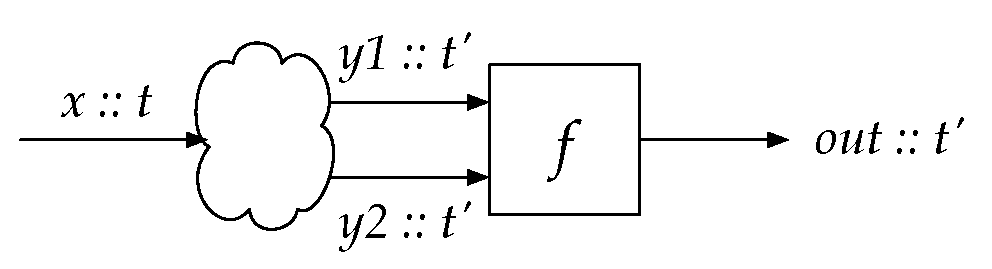
\includegraphics[width=0.6\textwidth]{images/latencyverify}
%\end{center}
%\caption{The function |f| used in a larger composition.} \label{fig:latencyverify}
%\end{figure}
%
%Whenever |f| is used in the circuit, we assume that both inputs of |f| are available at the same time.
%Moreover, both |y1| and |y2| of |f| must be subject to the same amount of latency in the entire circuit.
%This means that, when |x| occurs at |t'|, then the same number of cycles must pass between |t'| and |t|.
%Figure \ref{fig:samelatency} shows the relation between the time variable |t'|, |t| and the clock frequency.
%
%\begin{figure}[H]
%\begin{center}
%\centering
%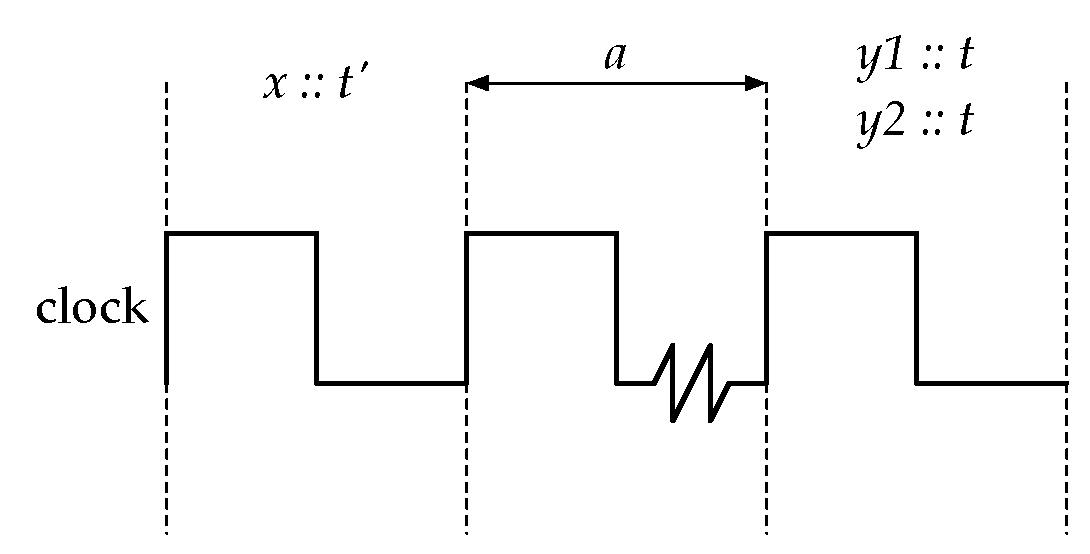
\includegraphics[width=0.6\textwidth]{images/samelatency}
%\end{center}
%\caption{Wawa} \label{fig:samelatency}
%\end{figure}
%
%As a result, whenever we insert memory elements between |x| and |y1,y2|, the same number of memory elements ought to be inserted between |x| and |y1|, and |x| and |y2|.
%So far we have assumed implicit placement of memory elements.
%Many compositions, which are not well-typed without implicit placement, can be made to be well-typed with implicit placement of memory elements.
%
%It is also possible to use explicit placement of memory elements.
%When using explicit memory elements, other aspects of time-dependent behaviour can be verified.
%To explain the difference between these two approaches, we first discuss implicit placement of memory elements, after which we will discuss explicit placement of memory elements.
%
%\subsection{Implicit Placement of Memory Elements}
%\begin{texexptitled}[text only]{Incorrect sampling definition.}{code:incorrectsampling}
%> incorrectSampling :: Int<t,t+1,t+2> -> Int<t+1>
%> incorrectSampling <x1,x2,x3> = x1 + x2 + x3
%\end{texexptitled}
%
%\begin{figure}[H]
%\begin{center}
%\centering
%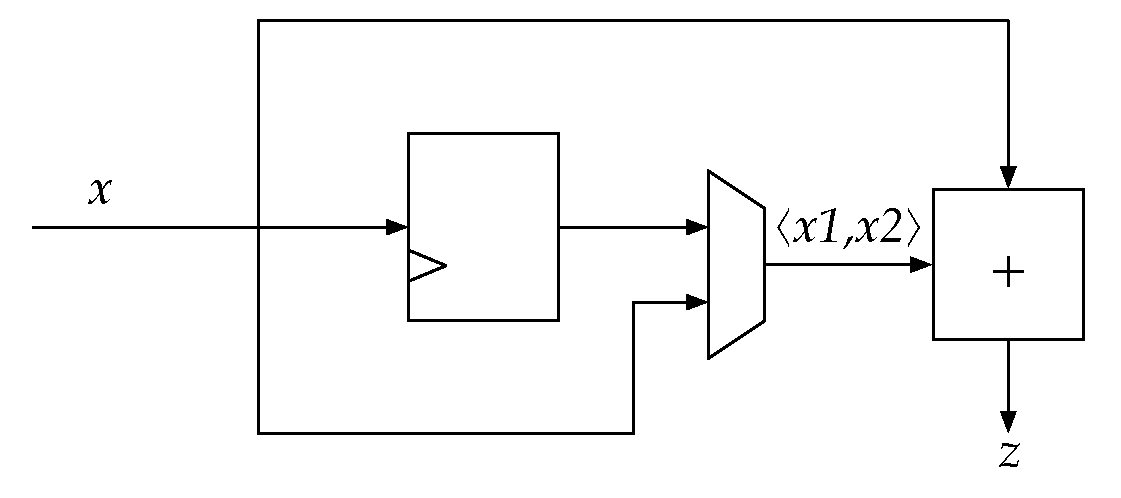
\includegraphics[width=0.6\textwidth]{images/compositioninc2}
%\end{center}
%\caption{Composition of |+|, |*| and |singleMem'|.} \label{fig:compositioninc2}
%\end{figure}
%
%\begin{texexptitled}[text only]{Correct composition.}{code:composition1cor}
%> composition'' x = z
%>   where   
%>           f :: Int<t> -> Int<2*t,2*t+1>
%>           f x   = <x,x>
%>           z     = (f x) + x
%\end{texexptitled}
%
%
%\subsection{Explicit Memory Elements}
%
%We discuss two approaches for inserting memory elements.
%The first approach is the least strict, in that \textit{any} amount of memory elements may be added to make the circuit function properly according to specification.
%So far we only defined individual functions, without reasoning about composing them.
%Individual functions can lead to incorrect specifications, as shown by the code of snippet \ref{code:incorrectsampling}.
%There, the |x3| is available at |<t+2>|, while the output is available at |<t+1>|.
%
%Since |incorrectSampling| is defined by the expression |x1 + x2 + x3|, the result of the composition can be available no sooner than |t+2|, as that is when |x3| is available.
%As a result, this specification is not well-typed.
%
%However, even when individual components are well-typed, compositions using those components do not have to be well-typed.
%In our extension of the type-system, time-dependent behaviour of individual components must always be maintained.
%For instance, when we represent combinational logic as a function with the type |Int<t> -> Int<t> -> Int<t>|, then the incurred latency for both inputs needs to be the same.
%\begin{texexptitled}[text only]{Incorrect composition.}{code:composition1inc}
%> (+) :: Int<t> -> Int<t> -> Int<t>
%> singleMem' :: Int<t> -> Int<t+1>
%> 
%> f :: Int<t> -> Int<t> -> Int<t+1>
%> f x y = (singleMem' x) + y)
%\end{texexptitled}
%
%\begin{figure}[H]
%\begin{center}
%\centering
%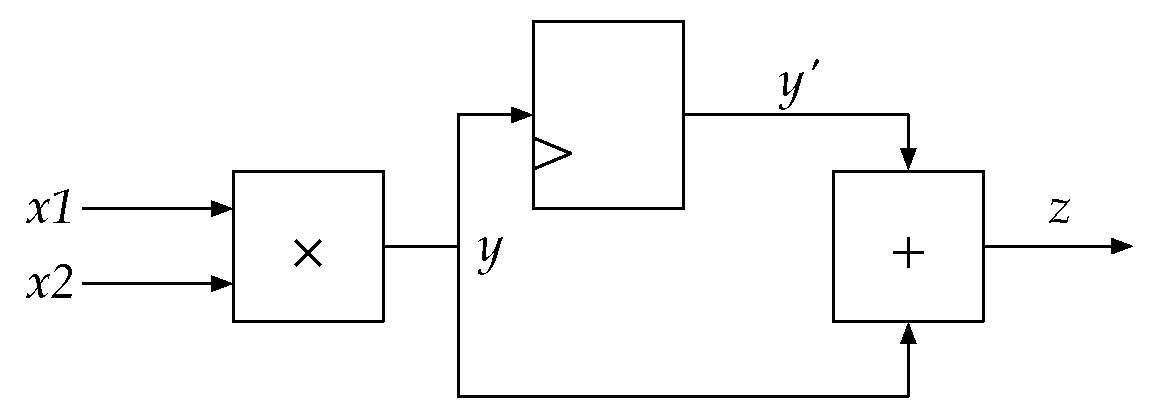
\includegraphics[width=0.6\textwidth]{images/compositioninc}
%\end{center}
%\caption{Composition of |+|, |*| and |singleMem'|.} \label{fig:compositioninc}
%\end{figure}
%
%\begin{texexptitled}[text only]{Incorrect composition.}{code:composition1inc}
%> (+) :: Int<t> -> Int<t> -> Int<t>
%> (*) :: Int<t> -> Int<t> -> Int<t>
%> singleMem' :: Int<t> -> Int<t+1>
%>
%> composition x1 x2 = 
%>   where   y   = x1 + x2
%>           y'  = singleMem' y
%>           z   = y * y'
%\end{texexptitled}
%
%\begin{texexptitled}[text only]{Correct composition.}{code:composition1cor}
%> composition' :: Int<t,t+1> -> Int<t,t+1> -> Int<t+1>
%> composition' x1 x2 = z
%>   where   y           = x1 + x2
%>           z           = f y
%>
%>           f :: Int<t,t+1> -> Int<t+1>
%>           f <y1,y2>   = y1 * y2 
%\end{texexptitled}
%
%\begin{texexptitled}[text only]{Correct composition.}{code:composition1cor}
%> composition' :: Int<t> -> Int<t> -> Int<t+1>
%> composition' x1 x2 = z
%>   where   y   = x1 + x2
%>           y'  = singleMem' y 
%>           z   = f y y'
%>
%>           f :: Int<t> -> Int<t+1> -> Int<t+1> 
%>           f   = (*)
%\end{texexptitled}

%In this chapter we will focus mainly on expressing timing constraints in source code.
%First we will briefly introduce basic syntax, operator precedence and type constructor precedence.
%Afterwards we will give a combined representation for type and time ascription, as well as providing a method to encode sequences as function arguments.
%Finally we will introduce some specific notation in creating feedback structures, as well as describing syntax which allows interactivity.
%
%Even though syntax is usually defined in pure ASCII form, we chose to typeset a few tokens to increase the readability.
%For instance, the |"->"| token is represented as $\rightarrow$, while angled brackets |"<"| \& |">"| are typeset as $\langle$ \& $\rangle$.
%
%\section{Basic Syntax}
%Since the semantics of our type-inference algorithm uses the $\lambda$-calculus, an obvious starting point for discussion of syntax are function definitions.
%Using let bindings we can introduce functions which are used multiple times within a single expression.
%When consider the top-level of a functional program, it generally consists of multiple functions used in different parts of the program.
%Each function has an identifier, which is simply a named variable of the $\lambda$-calculus.
%For instance, when we refer to the function |id x = x|, then |id| is variable name within a certain scope, which represents a function with type |X -> X|.
%The definition of |id x = x| represents $\lambda$-abstraction in the $\lambda$ calculus in the form of $id = \lambda x.x$.
%
%We can represent top-level functions by using nested let-bindings. 
%For instance, the code 
%\begin{changemargin}{1cm}{0cm}
%\begin{expansionno}{text only}%{On the $\lambda$-calculus}{exp:lambda}
%\begin{code}
%foo x = x + x
%
%bar x = x * x
%
%main x  =   let   y = foo x
%            in    bar y
%\end{code}
%\end{expansionno}
%\end{changemargin}
%could be translated to a \textit{nested} let-binding as follows
%\begin{changemargin}{1cm}{0cm}
%\begin{expansionno}{text only}%{On the $\lambda$-calculus}{exp:lambda}
%\begin{code}
%main x  =   let foo x = x + x
%            in  let bar x = x * x
%                in  let   y = foo x
%                    in    bar y
%\end{code}
%\end{expansionno}
%\end{changemargin}
%
%This shows how top-level definitions can be translated using let-bindings when we consider let-polymorhism.
%Using the |main| function to identify the top-level function, all other functions can be translated as part of the let-binding.
%As shown, we allow \textit{shadowing} of variables, meaning we can introduce a variable using the same identifier as a variable introduced in a higher scope.
%
%Of course, the definition of |foo| might have used |bar| or vice versa.
%When |foo| uses |bar|, we must introduce |foo| in a let-binding before we can introduce |bar|.
%This means that we must figure out the proper ordering in which to introduce functions in nested let-bindings.
%The ordering can be easily derived when parsing the code however, something which we do not focus on here.
%
%While let-bindings are useful, nesting let-bindings are difficult to read when complexity of descriptions increases.
%For this purpose we can allow multiple bindings within a single scope.
%For instance, in the above code the scope of |bar| is nested one level deeper than the scope of |foo|.
%Using multiple bindings in one let-binding we can introduce |foo| and |bar| within a single scope:
%\begin{changemargin}{1cm}{0cm}
%\begin{expansionno}{text only}%{On the $\lambda$-calculus}{exp:lambda}
%\begin{code}
%main x  =   let foo x = x + x
%                bar x = x * x
%            in  let   y = foo x
%                in    bar y
%\end{code}
%\end{expansionno}
%\end{changemargin}
%
%As can be seen from the examples so far, multiple bindings within the scope of a single let-statement need us to determine which definitions belong to which scope.
%In the example above we can see that |bar| can only realistically exist in the same scope as |foo|.
%However, we must define how we can determine to which scope an expression belongs in order to parse such expressions.
%The off-side rule allows us to define when a new scope begins solely by \textit{indentation} of a term.
%For instance, in the above example foo and bar have similar amounts of indentation, meaning they belong to the same scope.
%Parsing source code which contains the off-side rule is difficult, however as we are only defining syntax here this is of no concern.
%An implementation including a parser could always revert to bracket notion for scoping, as used more imperative languages such as C.
%
%\subsection{Type Ascription}
%In Haskell, type ascription is done using the |::| operator.
%The |::| operator accepts an identifier on the left hand side, and a type on the right hand side.
%The |::| operator is essentially a function which informs the type-system on what type we expect a variable to have.
%For instance, the identity function can be \textit{restricted} to only |Int| types when ascribed with the proper type, as shown below.
%\begin{changemargin}{1cm}{0cm}
%\begin{expansionno}{text only}%{On the $\lambda$-calculus}{exp:lambda}
%\begin{code}
%id :: Int -> Int
%id x = x
%\end{code}
%\end{expansionno}
%\end{changemargin}
%
%Type ascription can also occur within a function.
%\begin{changemargin}{1cm}{0cm}
%\begin{expansionno}{text only}%{On the $\lambda$-calculus}{exp:lambda}
%\begin{code}
%main x y =  let id z = z
%            in (id x) + ((id :: Int -> Int) y)
%\end{code}
%\end{expansionno}
%\end{changemargin}
%, which shows that the type of |id|, which is |X -> X| under let-polymorphism, is restricted to |Int -> Int| for the second usage when applied to |y|.
%
%Let-polymorphism allows us to define polymorphic functions.
%However, we can also restrict polymorphism using ascription by naming the type variables.
%In Haskell this is done using lower-case letters, to distingush them from type constructors which start with a capital letter.
%Here we follow the same approach, where usage of lower-case letters in ascription automatically introduces the type variables.
%For instance, in the code
%\begin{changemargin}{1cm}{0cm}
%\begin{expansionno}{text only}%{On the $\lambda$-calculus}{exp:lambda}
%\begin{code}
%choose :: a -> a -> a -> a
%choose x y z = if z then x else y
%\end{code}
%\end{expansionno}
%\end{changemargin}
%we restrict the types of |x|, |y| and |z| to be equal, regardless what these types may be.
%Since the |if then else| statement only accepts values of the boolean type, the other arguments are similarly restricted to boolean types. 
%In Haskell type variables have limited scope; type variables are only valid within the ascription they are used in.
%In our syntax we assume type variables to behave according to the same scoping rules as regular variables.
%This means they can be \textit{shadowed} by variables in a nested scope, but are available to all nested scopes if not shadowed.
%The same behaviour is also available in Haskell through the ``ScopedTypeVariables'' extension of GHC.
%
%\subsection{Function Application and Precedence}
%As in Haskell, function can be used in an infix manner.
%When defining a function such as |++|, shown below, we would like to use it infix whenever possible.
%When we define a function such as |++|, together with its type, then the parentheses indicate that this is regarded as an infix term.
%\begin{changemargin}{1cm}{0cm}
%\begin{expansionno}{text only}%{On the $\lambda$-calculus}{exp:lambda}
%\begin{code}
%(++) :: Int -> Int -> Int
%x ++ y = x + (y + y)
%\end{code}
%\end{expansionno}
%\end{changemargin}
%
%As shown, we have not defined the associativity of application.
%Whenever we apply a function we consider the application operation to be left associative.
%In the code snippet below
%\begin{changemargin}{1cm}{0cm}
%\begin{expansionno}{text only}%{On the $\lambda$-calculus}{exp:lambda}
%\begin{code}
%foo x = x + x
%bar x = x * x
%main x = bar foo x
%\end{code}
%\end{expansionno}
%\end{changemargin}
%, |bar foo x| is interpreted as |(bar foo) x|. 
%As bar uses a multiplication operation this would give a type error, as we are trying to multiply a function with itself.
%Brackets are needed in order to indicate the exact intention.
%Here the definition of |main| would have to be changed to |main x = bar (foo x)| in order to work properly.
%
%Similarly, type constructors are right associative.
%This means that a function with type |Int -> Int -> Int| is actually interpreted as |Int -> (Int -> Int)|, meaning the result of the first application is another function.
%
%\section{Time Representation}
%In order to concisely define a function's type and timing behaviour we will first define ascription involving both time and types.
%From a semantical point of view we do not distinguish between functions and other values when discussing time constraints.
%Whenever we have a function such as |Int -> (Int -> Int)|, we can ascribe each function with a time variable.
%For instance, we could define the entire function to exist at |t|. 
%When applied to a value this creates another function, which exists at (for example) |t+1|. 
%Finally, when applied to another value the final result is available at |t+2|.
%We can relate each subsequent value with a time variable as follows:
%\begin{changemargin}{1cm}{0cm}
%\begin{expansionno}{text only}%{On the $\lambda$-calculus}{exp:lambda}
%\begin{code}
%Int -> (Int -> Int)   @ t
%Int -> Int            @ t + 1
%Int                   @ t + 2
%\end{code}
%\end{expansionno}
%\end{changemargin}
%
%In order to ascribe each individual function with this time behaviour we use the same $\langle$ and $\rangle$ brackets as we used for introducing sequences in the previous chapter.
%Using the angled brackets we can ascribe each type with a time variable.
%Since we do not distinguish between functions and other values from the timing perspective, we consider the following definition
%\begin{changemargin}{1cm}{0cm}
%\begin{expansionno}{text only}%{On the $\lambda$-calculus}{exp:lambda}
%|Int<t> -> Int<t + 1> -> Int<t+2>|
%\end{expansionno}
%\end{changemargin}
%equivalent to
%\begin{changemargin}{1cm}{0cm}
%\begin{expansionno}{text only}%{On the $\lambda$-calculus}{exp:lambda}
%|(Int -> (Int -> (Int <t+2>))<t+1>)<t>|
%\end{expansionno}
%\end{changemargin}
%
%In the latter case we ascribe every partially applied function a specific time variable.
%Whenever time variables are equivalent, as in |Int<t> -> Int<t> -> Int<t>|, then the former definition is equivalent to |(Int -> Int -> Int)<t>|.
%To distinguish between regular type ascription and the introduced combination, we introduce the |:@| operator.
%Like the |::| operator, the |:@| operator accepts a variable name on the left hand side, while accepting a type-time combination on the right hand side.
%As an example, we define a timed adder below.
%\begin{changemargin}{1cm}{0cm}
%\begin{expansionno}{text only}%{On the $\lambda$-calculus}{exp:lambda}
%\begin{code}
%f :@ Int<t> -> Int<t + 1> -> Int<t+2>
%f x y = x + y
%\end{code}
%\end{expansionno}
%\end{changemargin}
%While types and timing combinations can be used, sometimes it is only needed to ascribe terms with timing information only.
%For this we use the |@| operator which, like type ascription, can be used within an expression.
%For instance, we can explicitly define registers as introduced in the previous chapter:
%\begin{changemargin}{1cm}{0cm}
%\begin{expansionno}{text only}%{On the $\lambda$-calculus}{exp:lambda}
%\begin{code}
%foo x y =   let x' = x @ t
%            in  (x' + y) @ t + 1
%\end{code}
%\end{expansionno}
%\end{changemargin}
%, in which |foo| would be equivalent to
%\begin{changemargin}{1cm}{0cm}
%\begin{expansionno}{text only}%{On the $\lambda$-calculus}{exp:lambda}
%\begin{code}
%foo :@ Int<t> -> Int<u> -> Int<t+1>
%foo x y = x + y
%\end{code}
%\end{expansionno}
%\end{changemargin}
%, where |u =< t + 1|.
%
%\section{Sequences}
%So far we have not discussed sequences.
%In the previous chapter we hinted at having a solution for using sequences as function arguments.
%Using the same syntax as above, we can define the following sampling code:
%\begin{changemargin}{1cm}{0cm}
%\begin{expansionno}{text only}%{On the $\lambda$-calculus}{exp:lambda}
%\begin{code}
%f :@ Int<t,t+1,t+2> -> Int<t+2>
%f <x,y,z> = x + y + z
%\end{code}
%\end{expansionno}
%\end{changemargin}
%
%In this example the output is the summation of three sequential values from a single wire.
%If we define the input as a stream of values $v = v_1,v_2,\ldots,v_n$, then the output would be defined no earlier than when $v_3$ is defined.
%The earliest output of the circuit would be $v_1 + v_2 + v_3$.
%However, in the next cycle, $x = y$, $y = z$ and $z = v_4$, which means that |f| samples the input in a sequential fashion.
%As shown, we use the definition of a sequence directly in the definition of the time-dependent behaviour of |f|.
%Part of the definition is the term |<x,y,z>|, which deconstructs a sequence consisting of three variables into the individual variables.
%When we deconstruct the sequence we can relate every variable with a timing expression.
%The above code could then be transformed as if accepting 3 individual arguments as follows:
%\begin{changemargin}{1cm}{0cm}
%\begin{expansionno}{text only}%{On the $\lambda$-calculus}{exp:lambda}
%\begin{code}
%f :@ Int<t> -> Int<t+1> -> Int<t+2> -> Int<t+2>
%f x y z = x + y + z
%\end{code}
%\end{expansionno}
%\end{changemargin}
%
%Sequence construction can be done using the bracket notation as well.
%\begin{changemargin}{1cm}{0cm}
%\begin{expansionno}{text only}%{On the $\lambda$-calculus}{exp:lambda}
%\begin{code}
%f :@ Int<t> -> Int<2t,2t+1>
%f x = <x,x+42>
%\end{code}
%\end{expansionno}
%\end{changemargin}
%Here, |f| accepts a single sample, which is used in a sequence.
%Sequences introduce upsampling, where the number of elements of the sequence relates the ratio between the input and the output samples.
%Here, the output produces two samples, while using only a single input.
%
%While the above syntax to create sequences is concise enough to describe upsampling, the same syntax may be too concise when individual elements of the sequence are important.
%This is the case when we consider feedback, where distinguishing the initial value of a register can be important.
%Sequences are not first-class in our language, but we introduce syntactic sugar from which it appears as if sequences are first class.
%In let-bindings we introduce variables and definitions of variables.
%To build a sequence we allow association of a single variable within a let-binding with multiple other expressions, as shown below.
%\begin{changemargin}{1cm}{0cm}
%\begin{expansionno}{text only}%{On the $\lambda$-calculus}{exp:lambda}
%\begin{code}
%f :@ Int<t> -> Int<0,t>
%f x =   let x'  @ 0       = 42 + x
%                @ t       = x' + x
%        in x'
%\end{code}
%\end{expansionno}
%\end{changemargin}
%
%The ordering in which subsequent definitions appear in the let-binding combined with ascription also defines the ordering of the sequence.
%

%include polycode.fmt 
%format |-> = "\mapsto"
%format veca = "\vec a"
%format vecb = "\vec b"
%format delay1 ="\sigma_1"
%format delayx ="\sigma_x"
%format delay = "\sigma"
%format Delayx = "\Delta_x"
%format Delay1 = "\Delta_1"
%format mylang = "\lambda^{\rightarrow}_{\Delta}"
%format psin = "\psi. n."
%format < = "\langle"
%format > = "\rangle"
%format *> = ">"
%format <--> = "\leftrightarrow"
%format <- = "\leftarrow"
%format -!> = "\overset{!}{\rightarrow}"
%format \\ = "\lambda"
%format <==> = "\leftrightarrow"
%format <||> = "\langle || \rangle"
%format par = "\langle || \rangle"

\chapter{A Temporal Type System} \label{ch:typesystem}
In the previous chapter, we have (informally) shown how representing time as part of the type system gives us the ability to reason about various forms of hardware and their compositions.
However, informal reasoning about temporal representation does not give any guarantees with regards to the feasibility of expressing time as part of the type system.

In this chapter, we define a grammar and a set of typing rules, which make a convincing case for the feasibility of expressing temporal behaviour as part of the type system.
To do so, we first define expressions and timed types.
Secondly, we introduce \textit{polytemporal types}, based on polytypes as introduced in section \ref{sec:polymorphiclambda}.
Third, we define constraints as per HM(X)\cite{odersky1999type}, which are used in the typing rules of our type system.
Finally, we show a number of derivations and briefly discuss the expressiveness of the given type system. 

\section{Grammar of $\lambda_t$}
The grammar of our language, which we call $\lambda_t$, is very similar to the languages discussed in chapter \ref{ch:background}.
Expressions $e$ consists of the usual terms of the $\lambda$-calculus: variables, abstraction and application.
We chose to also represent constants and the meta-function $\delta$.
The $\delta$ meta-function is used to introduce delays within function types.
Introduction of delays is severly restricted however, which is why we explain its mechanics later in this chapter, together with reasoning as to \textit{why} it is severly restricted.
 
\begin{definitiontitled}[text only,float]{Expressions}{def:tt-exp}
\begin{minipage}[b]{0.50\linewidth}
\begin{tabular}{lclr}
$e$     & $\Coloneqq$ &                                         & expressions:            \\
        & |    & $x$                                            & \textit{(variable)}     \\
        & |    & $\lambda x.e$                                  & \textit{(abstraction)}  \\
        & |    & $e \: e$                                       & \textit{(application)}  \\
        & |    & $c$                                            & \textit{(constant)}     \\
        & |    & $\delta(e,n \in \mathbb{N}_0)$                                  & \textit{(delay)}        \\
\end{tabular}
\end{minipage}
\begin{minipage}[b]{0.40\linewidth}
\begin{tabular}{lclr}
c       & $\Coloneqq$ &                                         & constants:                  \\
        & |    & true                                           & \textit{(Boolean true)}     \\
        & |    & false                                          & \textit{(Boolean false)}    \\
        & |    & n $\in \mathbb{Z}$                             & \textit{(Integer literals)} \\
\end{tabular}
\end{minipage}
\end{definitiontitled}

The constants which we allow are either of the \textit{Boolean} variety, or the \textit{Integer} variety.
Having the ability to define different types of constants allows us to easily show that our type-system also includes regular type-checking over base types.
Furthermore, even though the system currently has no term which directly represents choice, the system could be easily extended with it when needed due to the existence of Boolean types.

We define the set of simple types $\tau$ below.
If needed, we also use the letter $\rho$ to range over simple types.
Like the simply typed $\lambda$-calculus, there exist only two ways in which a simple type can be constructed.
A function type can be constructed using the $\to$ type-constructor, while a \textit{timed type} can be constructed by combining a \textit{time expression} $\epsilon$ and a base type $T$.

\begin{definitiontitled}[text only,float]{Types}{def:tt-type}
\begin{minipage}[b]{0.50\linewidth}
\begin{tabular}{lclr}
$\tau$  & $\Coloneqq$ &                                         & simple types:               \\
        & |           & $\tau \rightarrow \tau$                 & \textit{(function type)}    \\
        & |           & $T \langle \epsilon \rangle$            & \textit{(timed type)}       \\
\end{tabular}
\end{minipage}
\begin{minipage}[b]{0.40\linewidth}
\begin{tabular}{lclr}
T       & $\Coloneqq$ &                                         & base types:                 \\
        & |           & \textit{Int}                            & \textit{(Integer type)}     \\
        & |           & \textit{Bool}                           & \textit{(Boolean type)}     \\
\end{tabular}
\end{minipage}
\begin{tabular}{lclr}
$\epsilon$ & $\Coloneqq$ & $ \epsilon + (a \in \mathbb{N}_0)$   & \textit{(time expression)}  \\
           & |           & $ t $                                & \textit{(time variable)}    \\
\end{tabular}
\end{definitiontitled}

Base types are similar to those used in the simply-typed $\lambda$-calculus, and are constructed by one of the type constants \textit{Bool} or \textit{Int}.
A base type tells us something about the form or shape of a value; either something is a number or a boolean value.
Time expressions consists of a \textit{variable} moment in time $t$, and one or more \textit{concrete} offsets to $t$.
Using $\tau$ we can define the type of a memory element which holds an integer as: $\textit{Int}\langle t \rangle \to \textit{Int}\langle t + 1 \rangle$.

We can now define the behaviour of $\delta$ informally as well.
The $\delta$ keyword accepts values with function types.
When the $\delta$ function is applied to a function with some offset $n$, then it adds the offset to every time expression occuring on the right-hand side of the type constructor $\to$.
For instance, given the identity function \[\lambda x.x : \textit{Int} \langle t \rangle \to \textit{Int} \langle t \rangle.\]
We apply $\delta(\lambda x.x,1)$, which results in the function \[\delta(\lambda x.x,1) : \textit{Int} \langle t \rangle \to \textit{Int} \langle t + 1 \rangle.\]
We discuss the full implications of this behaviour later in this chapter.

Time variables, like type variables in Damas-Milner, are \textit{monomorphic} and range over the set of natural numbers $\mathbb{N}_0$.
To describe hardware, we need to be able to define hardware components which are \textit{polytemporal}, e.g. work for clock cycles $0,1,\ldots,n$.
For this we introduce a \textit{polytemporal type} in definition \ref{def:timescheme}, similar to polytypes of Damas-Milner.

\begin{definitiontitled}[text only,float]{Polytemporal types}{def:timescheme}
A \textit{polytemporal type} $\sigma$, written as 
\[ \sigma = \forall t.\tau \quad (\textit{ftv}(\tau) = \{t\})\]
, consists of universal quantification over a single time variable $t$, which is bound in the simple type $\tau$.
Moreover, there are no free time variables in $\tau$ other than $t$.
\end{definitiontitled}

Every value is defined in terms of some time variable $t$.
This means that, unlike other type systems which include some form of polymorphism, types are \textit{always} polytemporal.
Literals are values which exist at every moment in time, expressed by their type: $42 : \forall t. T\langle t \rangle$.
Similarly, variables are polytemporal as well.
Without any restriction, all values can exist at any $t \in \mathbb{N}_0$, which is not exactly useful.
Restrictions on time variables are needed to \textit{limit} the existence of values.
For instance, by applying a function which represents a single memory element to a constant value, the \textit{resulting} value can only exist at every clockcycle $> 0$. 
To be able to restrict existence of values, we introduce \textit{constraints} below.

\section{Constraints}
Constraints consists of existential quantification of time variables, which are used as binders for the time variables used in time expression constraints.
Time expression constraints can be used to restrict a certain time expression in terms of another.
Time expression constraints are inequalities with good reason; usage of equalities would restrict the expressiveness of the type system more than is needed.
This is explained later in greater detail.

\begin{definitiontitled}[text only,float]{Constraints}{def:tt-constraint}
We define the \textit{constraint} $C$ as follows:\\
\begin{tabularx}{0.75\textwidth}{lc X lr}
$C$     & $\Coloneqq$ &                           & & constraints:                          \\
        & |           & $\exists t. C$            & & \textit{(existential constraint)}     \\
        & |           & $C \land C$               & & \textit{(composition)}                \\
        & |           & $\epsilon \leq \epsilon$  & & \textit{(time expression constraint)} \\
        & |           & T $=$ T                   & & \textit{(base type constraint)}       \\
        & |           & $\tau \equiv \tau$        & & \textit{(type equivalence constraint)}\\
        & |           & true                      & & \textit{(satisfied constraint)}       \\
        & |           & false                     & & \textit{(non-satisfied constraint)}   \\
\end{tabularx}\\
, which can be used to define both type constraints as time constraints.
\end{definitiontitled}

It may seem strange to have both existential quantification of time variables and universal quantification in the same type system.
However, the constraints $C$ are created separately from polytemporal types, and as a result, needs its own binders.
This approach is not new; HM(X) uses the same approach to reason about polymorphism.

In the constraints we have inequalities on time expressions, and equalities on base types.
Restrictions on base types are not strictly needed to show the merit of our type system with regards to reasoning about temporal behaviour.
We have included restrictions on base types to show that the combination of time expressions and base types can indeed be reasoned about within the same system.
Additionally, the type equivalence constraint requires that types must be equal under $\alpha$-conversion.
These different forms of constraints are needed in order to reason about the time-dependent behaviour, and will be explained in more detail later.

Other constraints include the trivial constraints ``true'', ``false'' and composition of constraints through logical conjuction ($\land$).
Composition of constraints including existential quantification needs to result in a well-formed constraint.
Even though the conjuction $\exists t_1.C_1 \land \exists t_2.C_2$ is correct from the above definition, it becomes tedious to make sure every time variable is quantified and in scope.
As a result, we define a constraint to be well-formed if every existential quantification is performed first, before introducing additional constraints.
In the typing rules presented later in this chapter, we assume that every constraint is well-formed.
When two constraints as $\exists t_1.C_1 \land \exists t_2.C_2$ are composed, all existential quantification is moved to the head of the constraint.

Together with the context $\Gamma$, constraints are used in type judgements of the form $C; \Gamma \vdash e : \forall t. \tau$.
The type judgment ought to be read as: we can derive from the context $\Gamma$ that the expression $e$ has the simple type $\tau$, for every $t$ such that the constraints in $C$ hold.

\begin{definitiontitled}[text only,float]{Constraints}{def:tt-context}
We define the context $\Gamma$ as follows:\\
\begin{tabularx}{0.75\textwidth}{lc X lr}
$\Gamma$& $\Coloneqq$ &                                         & contexts:           \\
        & |     & $\emptyset$                                   & (empty context)     \\
        & |     & $\Gamma,x:\tau$                               & (type binding).     \\
\end{tabularx}\\
\end{definitiontitled}

Without typing rules it is difficult to create an example which shows how constraints can be used to reason about the existence of values.
To do so, we postpone showing a full type derivation here, and focus on how constraints can be used.
Suppose we have a function \textit{register} with the polytemporal type 
\[\textit{register} : \forall t. \textit{Int}\langle t \rangle \to \textit{Int}\langle t + 1 \rangle.\]
Now, without any constraint, this function can be used to transform any \textit{Int} of any $t \in \mathbb{N}_0$ to an \textit{Int} at $t+1$.
When \textit{register} is applied to a value, as in $v = \textit{register} \: 42$, the resulting value $v$ exists one clockcycle later than the value \textit{register} is applied to.
All this can be expressed without any constraint, as the value simply has type 
\[v : \forall t. \textit{Int}\langle t + 1 \rangle.\]
However, when we apply another function (called \textit{foo}) to $v$, the constraint that $v$ can only exists at $t \geq 1$ must be adhered to.
Suppose \textit{foo} has type: \[\textit{foo} : \forall t'. \textit{Int}\langle t' \rangle \to \textit{Int}\langle t' + 1 \rangle \to \textit{Int}\langle t' + 2 \rangle.\]
When applied to $v$, as in $v' = \textit{foo} \: v$, the resulting function has type \[\textit{foo} \: v : \forall t'. \textit{Int}\langle t' + 1 \rangle \to \textit{Int}\langle t' + 2 \rangle.\]
However, this does \textit{not} work for every $t'$, as the first argument of \textit{foo} does not exist at $t' = 0$.
By adding the constraint \[\exists t. \exists t'. t + 1 \leq t'\], we can be sure that, when the constraint holds, $t'$ is not equal to $0$.
If it were, then there would have to exist a $t$ such that $t+1 \leq 0$. 
As $t \in \mathbb{N}_0$, this is obviously incorrect.

It may seem odd at this point why we chose inequalities over equalities, as equalities would lead to the same result.
However, consider the function resulting from $\textit{foo} \: v$.
If we were to apply it to $v$ again, as in $v'' = (\textit{foo} \: v) \: v$, then the resulting constraint \[\exists t. \exists t'. t + 1 = t' \land t + 1 = t' + 1\] could never hold.
Yet, this application is \textit{valid}.
Memory elements can be used to delay a value indefinitely.
With inequalities we can express this as part of the constraint: \[ \exists t. \exists t'. t+1 \leq t' \land t+1 \leq t'+1.\]
From this constraint we can derive that, in order for the composition of $v''$ to work, a memory element has to be added for the \textit{second} $v$, before applying $\textit{foo} \: v$ to it.
We can derive this by solving the constraints for the minimal value of $t$ and $t'$.
From the constraints we derive $t = 0$ and $t' = 1$.
Plugging these into the known types of \textit{foo} and \textit{register}, allows us to determine when a memory element needs to be added.
For instance, $v$ exists at $1$ if $t=0$, and \textit{foo}'s second argument is expected at $t' + 1$, which is $2$ if $t' = 1$.
The difference between $v$ and the type of the second argument of \textit{foo}, indicates that something must be added here in order to make the composition work.
This also makes sense intuitively.
The type of \textit{foo} indicates that it \textit{expects} the second argument to exist one clock cycle later than the first.
When applied to the same value twice, something must be done to one of the values in order to make the composition work.

\section{Typing Rules}
Now that we introduced constraints, we can introduce the typing rules which give us the ability to (re)construct and verify expressions of $\lambda_t$.
Before doing so however, we provide a relation between two simple types below, in order to simplify the definition of typing rules.
In particular, this type relation is used to create the constraints which are introduced by function application.

\begin{definitiontitled}[text only,float]{The type relation $\preceq$}{def:preceq}
We define the precedence relation $\preceq$ as
\[\tau_1 \preceq \tau_2 = \left\{ 
  \begin{array}{l l}
      \epsilon_1 \leq \epsilon_2 \land \text{T}_1 = \text{T}_2
    & \text{if $\tau_1,\tau_2 = T_1 \langle \epsilon_1 \rangle, T_2 \langle \epsilon_2 \rangle$ }\\
      \tau_1 \equiv \tau_2
    & \text{if $\tau_1,\tau_2 = \tau_{11} \to \tau_{12} \land \tau_{21} \to \tau_{22}$}\\
      \text{false}
    & \text{otherwise}\\
  \end{array} \right.
\]
, where $\tau_1$ temporally precedes $\tau_2$ and the base types of $\tau_1$ and $\tau_2$ are equal.
\end{definitiontitled}

The $\preceq$ relation distinguishes three cases to do so.
In the first case, a relation between two timed types is created.
As explained in the previous section, relations between time expressions are inequalities.

The second case defines type equality under $\alpha$-conversion.
This case is used to define the precedence relation for function types.
To show why we use equivalence here, instead of defining a ``real'' precedence relation for function types, we show the two most obvious ways to represent function precedence, and why they do not work.

First, we define the relation $\tau_1 \preceq \tau_2 = \tau_{11} \preceq \tau_{21} \land \tau_{12} \preceq \tau_{22}$, where $\tau_1 = \tau_{11} \to \tau_{12}$ and $\tau_2 = \tau_{21} \to \tau_{22}$.
In this case, $\tau_1$ must precede $\tau_2$. 
When $\tau_2$ represents the type of a function which is expected, then $\tau_1$ represents the type of a function which is actually supplied.
By applying the type inequality pointwise for every timed type in $\tau_1$ and $\tau_2$, we state that the supplied function may expect the supplied values \textit{earlier} than the expected function.
Even though the constraints would reflect that condition if it occurs, by using this precedence relation additional memory elements could be inserted through reckless use of higher order functions.

The same precedence relation could be inverted.
However, this is also problematic, as there is no guarantee that the supplied function results in a value, before that actual value is needed.
Again, the constraints would reflect that condition, and more memory elements could be inserted if this condition occurs.
However, as we already have a certain amount of automatic introduction of memory elements, we restrict the type of higher order functions to match \textit{exactly} with the expected function type.

Finally, the third case is used for cases where types do not match. 
Even though this case might seem superfluous when compared to the second, the third case is needed in order to restrict usage of sequences, which we discuss later in this chapter.

\subsection{The Typing Rules TT-Var, TT-Const \& TT-Gen}
Finally, we define and discuss the typing rules.
We start by the rule TT-Var, which is similar to the rules involving variables discussed in chapter \ref{ch:background}.

\begin{definitiontitled}[text only]{Typing rules of $\lambda_t$ (a)}{def:typerules}
\begin{tabularx}{\textwidth}{ r r X r r}
\centering
$ \displaystyle 
  \frac{  \Gamma(x) = \tau
  }{      \text{true}; \Gamma \vdash x : \tau }
$ &
TT-Var
&
&
\centering
$ \displaystyle
\frac{ 
} { C; \Gamma \vdash c : \tau }
$ &
TT-Const \\
\end{tabularx}\newline
\begin{tabularx}{\textwidth}{X r l X}
&
$ \displaystyle
  \frac{ C; \Gamma \vdash e : \tau \quad \textit{ftv}(\tau) = t 
  }{     \exists t. C; \Gamma \vdash \forall t.\tau }
$ 
& TT-Gen 
& \\
\end{tabularx}
\end{definitiontitled}

When $\Gamma(x) = \tau$, then we can conclude from $\Gamma$, without constraint, that $x : \tau$.
We use this to define the type of $x$ in $\Gamma_0$ as follows:
\begin{prooftree}
\AxiomC{$\Gamma_0(x) = \textit{Int}\langle t_0 \rangle$}
\RightLabel{\scriptsize{(1)}}
\UnaryInfC{true;$\Gamma_0 \vdash x : \textit{Int}\langle t_0 \rangle$.}
\end{prooftree}

As shown, the TT-Var rule does not introduce universal quantification over $t_0$.
We apply TT-Gen, which transforms an expression $e$ with type $\tau$, to a polytemporal type.
A restriction on TT-Gen is that all free variables in $\tau$ are equal to $t$, in order to allow universal quantification over $t$.
Since the definition of $\tau$ does not include a binder for time variables, all time variables in $\tau$ are free.
This means that, after applying this rule, $e : \forall t.\tau$, no time variables other than $t$ are used in $\tau$.

Additionally, we add the constraint $\exists t.$, without modifying the existing constraint.
Existential quantification in the constraint provides us with a binder to add inequalities of time expressions.
It is however difficult to see that, if there exists a $t$ such that the constraints in $C$ hold, $e$ has the type $\forall t.\tau$.
As mentioned earlier, the universal quantification is subject to the constraints in $C$.
If the constraints in $C$ do not hold for a particular $t$, then $e$ is not well-typed for that particular $t$.
If we assume $C = \text{true}$, then any $t \in \mathbb{N}_0$ can be chosen. 

We use the definition of $\Gamma_0$ from {\scriptsize{(1)}}, to derive the polytemporal type of $x$.
\begin{prooftree}
\AxiomC{true;$\Gamma_0 \vdash x : \textit{Int}\langle t_0 \rangle$}
\RightLabel{\scriptsize{(2)}}
\UnaryInfC{$\exists t_0.$true;$\Gamma_0 \vdash x : \forall t_0. \textit{Int}\langle t_0 \rangle$}
\end{prooftree}

\subsection{The Typing Rule TT-Abs}
Next, we define TT-Abs.
This rule is rather involved, for two reasons:
\begin{enumerate*}
 \item  polytemporal types only consist of a single time variable, so the types of $x$ and $e$ need to be changed via $\alpha$-conversion to use a new time variable;
 \item  if $x$ is used within $e$, then the constraints the types of $x$ and $e$ are subject to are known, yet the exact relation between $x$ and $y$ cannot be determined from their types alone.
\end{enumerate*}

\begin{definitiontitled}[text only]{Typing rules of $\lambda_t$ (b)}{def:tt-abs}
\centering
\begin{tabular}{ r l }
$ \displaystyle 
  \frac{  C; \Gamma \vdash x : \forall t_1.\tau_1 \quad C; \Gamma \vdash e : \forall t_2. \tau_2 \quad t_3 \notin \textit{vars}(C,\Gamma)
  }{      \exists t_3. C \land t_3 \leq t_1 \land t_2 \leq t_3+a;\Gamma \vdash \lambda x. e : \forall t_3. [t_3/t_1]\tau_1 \to [t_3 + a/t_2]\tau_2 }
$
& TT-Abs \\
\end{tabular}
\end{definitiontitled}

Given that $x$ is used within $e$, we can determine the exact difference in the time expressions of $x$ and $e$ based on the constraints they are subject to.
From this difference we can, in principle, determine an offset $a$ such that a fresh time variable $t_3 \leq t_1$ and $t_2 \leq t_3 + a$.
When this is the case, we say the resulting abstraction \textit{encloses} $x$ and $e$.

Similar to Damas-Milner, we cannot determine from types alone what the new type of $\lambda x.e$ ought to be.
Like algorithm $W$ in the case of Damas-Milner, we need an algorithm which finds the smallest $a$ such that $\lambda x. e : \forall t_3.[t_3/t_1]\tau_1 \to [t_3 + a/t_2]\tau_2$ encloses $x : \forall t_1.\tau_1 $ and $e : \forall t_2. \tau_2$. 
We discuss the options of solving for $a$ in the next section.

Using the derivation of {\scriptsize (2)}, we derive the type of the identity function $\lambda x.x$.
Since we derive the identity function here, $e = x$, which results in two identical premises for the rule TT-Abs.
For simplicity' sake, we only include the single premise here.

\begin{prooftree}
\AxiomC{$\exists t_0.$true;$\Gamma_0 \vdash x : \forall t_0. \textit{Int}\langle t_0 \rangle$}
\RightLabel{\scriptsize (3)}
\UnaryInfC{$\exists t_1.\exists t_0. t_1 \leq t_0 \land t_0 \leq t_1 + a;\Gamma_0 \vdash \lambda x.x : \forall t_1. \textit{Int} \langle t_1 \rangle \to \textit{Int} \langle t_1 \rangle$}
\end{prooftree}
We take $a=0$ and simplify this expression for presentation purposes by removing the constraint $t_1 \leq t_0 \land t_0 \leq t_1 + a$, which implies $t_1 = t_0$.
The resulting type judgement reads:
\[\exists t_0.\text{true;}\Gamma_0 \vdash \lambda x.x : \forall t_0. \textit{Int} \langle t_0 \rangle \to \textit{Int} \langle t_0 \rangle.\]

In the example of {\scriptsize (3)}, $e$ is equal to $x$, which greatly simplifies the derivation. 
After introducing the remaining typing rules we will show another derivation, where $e$ and $x$ are different.

\subsection{The Typing Rule TT-Delta}
To introduce delays, TT-Delta applies a positive shift to time expression of the right hand side of a function type.
\begin{definitiontitled}[text only]{Typing rules of $\lambda_t$ (c)}{def:tt-delta}
\centering
\begin{tabular}{l l}
$ \displaystyle
\frac{ C;\Gamma \vdash e : \forall t. \tau \rightarrow \rho 
} { C;\Gamma \vdash \delta(e,n) : \forall t. \tau \rightarrow [t+n/t]\rho}
$ &
TT-Delta\\
\end{tabular}
\end{definitiontitled}

As a result, function types always have an increasing delay as more $\to$ type constructors are nested.
Given a function type, the TT-Delta rule only delays the type of the result, whether that is another function type or a timed type.
Using the result of {\scriptsize (3)}, we derive the type of a function which represents a single memory element as follows.

\begin{prooftree}
\AxiomC{$\exists t_0.$true;$\Gamma_0 \vdash \lambda x.x : \forall t_0. \textit{Int}\langle t_0 \rangle \to \textit{Int}\langle t_0 \rangle$}
\RightLabel{\scriptsize (4)}
\UnaryInfC{$\exists t_0.$true;$\Gamma_0 \vdash \delta(\lambda x.x,1) : \forall t_0. \textit{Int}\langle t_0 \rangle \to \textit{Int}\langle t_0 + 1 \rangle$ }
\end{prooftree}

\subsection{The Typing Rule TT-App}
Functions can be applied to other values.
In the rule TT-App, we define that $e_1$ must have a function type, and $e_2$ has a type which is unrelated to $e_1$.
\begin{definitiontitled}[text only]{Typing rules of $\lambda_t$ (d)}{def:tt-app}
\centering
\begin{tabular}{l l}
$ \displaystyle
  \frac{  C_1; f : \forall t_1. \textit{Int}\langle t_1 \rangle \rightarrow \textit{Int}\langle t_1 + 1 \rangle \quad \quad C_2; v : \forall t_2. \textit{Int}\langle t_2 \rangle
  } {     \textit{Int} = \textit{Int} \land t_2 \leq t_1 \vdash f \: v : \forall t_1. \textit{Int}\langle t_1 + 1 \rangle } 
$ 
& TT-App \\
\end{tabular} 
\end{definitiontitled}

This is contrary to how other languages define function application, where $\tau_2 = \tau_{11}$.
Instead, we state that $\tau_2 \preceq \tau_{11}$.
Intuitively speaking, we can apply a function to a value when the value exists, as long as the value exists before the function ``expects'' it to exist.
If the value exists one or more clockcycles before the function expects it to exist, we can use memory elements to delay the value to the point where the function expects it.

To show how this typing rule works, we take the derivation of $\Gamma_0$ from {\scriptsize (1)} and {\scriptsize (2)} to similarly derive the type of $y$.
We then apply the function of {\scriptsize (4)} to $y$, leading to a set of constraints as follows.
\begin{prooftree}
\AxiomC{$\exists t_0.$true;$\Gamma_0 \vdash \delta(\lambda x.x,1) : \forall t_0. \textit{Int}\langle t_0 \rangle \to \textit{Int}\langle t_0 + 1 \rangle$}
\AxiomC{$\Gamma_2(y) = \textit{Int}\langle t_2 \rangle$}
\UnaryInfC{true;$\Gamma_2 \vdash y : \textit{Int}\langle t_2 \rangle$}
\UnaryInfC{$\exists t_2.$true;$\Gamma_2 \vdash y : \forall t_2. \textit{Int}\langle t_2 \rangle$}
\RightLabel{\scriptsize (5)}
\BinaryInfC{$\exists t_0,t_2.t_2 \leq t_0 \land \textit{Int} = \textit{Int}$;$\Gamma_0 \cup \Gamma_2 \vdash \delta(\lambda x.x,1) y : \forall t_0. \textit{Int}\langle t_0 + 1 \rangle$}
\end{prooftree}

\subsection{Other Derivations}
To show a more involved example, we use the application $\delta(\lambda x.x,1) \: y$ from {\scriptsize (5)} to create a function of $y$.
As shown in {\scriptsize (5)}, one register is applied to $y$.
As a result, the abstraction of $\lambda y. \delta(\lambda x.x,1) \: y$ would have the same type as the expression in derivation {\scriptsize (4)}.
To create a more meaningful derivation, we create another shifted identity function $\delta(\lambda z.z,1)$, which is derived similarly to {\scriptsize (4)}, to create the following expression:
\[ \lambda y.\delta(\lambda z.z,1) \: (\delta(\lambda x.x,1) \: y),\]
which delays the argument $y$ of type \textit{Int} twice.

To keep the typing rules readable, we define the following shorthands, which are derived from {\scriptsize (1)} to {\scriptsize (5)}.
\[ \begin{array}{l r} 
      C_2 = \exists t_0,t_2.t_2 \leq t_0 \land \textit{Int} = \textit{Int} & \text{\scriptsize derived from (4)}\\
      C_3 = \exists t_3.\text{true} & \text{\scriptsize derived from (2)}\\ 
      e_3 = \delta(\lambda z.z,1) \: (\delta(\lambda x.x,1) \: y) & \text{\scriptsize derived from (5) and (2)}\\
      \Gamma_4 = \Gamma_0 \cup \Gamma_2 & \text{\scriptsize derived from (5)}\\
   \end{array}
\]

The constraint $C_3$ is associated with $\delta(\lambda z.z,1)$, which has type $\forall t_3. \textit{Int}\langle t_3 \rangle \to \textit{Int}\langle t_3 + 1\rangle$.
We use the above definitions to derive the following:

\begin{prooftree}
\AxiomC{$C_3;\Gamma_3 \vdash \delta(\lambda z.z,1) : \forall t_3. \textit{Int}\langle t_3 \rangle \to \textit{Int}\langle t_3 + 1 \rangle$}
\AxiomC{$C_2;\Gamma_4 \vdash \delta(\lambda x.x,1) y : \forall t_0. \textit{Int}\langle t_0 + 1 \rangle$}
\RightLabel{\scriptsize (6)}
\BinaryInfC{$C_1 \land C_2 \land \textit{Int}\langle t_0 + 1 \rangle \preceq \textit{Int}\langle t_3 \rangle; \Gamma_4 \vdash e_3 : \forall t_3. \textit{Int} \langle t_3 + 1 \rangle$}
\end{prooftree}

In {\scriptsize (6)} we defined two memory elements, and applied them to $y$.
We use this definition to show how the abstraction of $y$ leads to the (correct) type $\forall t_4. \textit{Int}\langle t_4 \rangle \to \textit{Int} \langle t_4 + 2 \rangle$.
We define $C_4 = C_1 \land C_2 \land \textit{Int}\langle t_0 + 1 \rangle \preceq \textit{Int}\langle t_3 \rangle$ and apply TT-Abs to it as follows.

\begin{prooftree}
\AxiomC{$C_4;\Gamma_4 \vdash e_3 : \forall t_3. \textit{Int} \langle t_3 + 1 \rangle$}
\AxiomC{$\exists t_2.$true;$\Gamma_2 \vdash y : \forall t_2. \textit{Int} \langle t_2 \rangle$}
\RightLabel{\scriptsize (7)}
\BinaryInfC{$\exists t_4.C_4\land t_4 \leq t_2 \land t_3 \leq t_4 + a;\Gamma_4 \vdash \lambda y.e_3 : \forall t_4. \textit{Int}\langle t_4 \rangle \to \textit{Int} \langle t_4 + a + 1 \rangle$}
\end{prooftree}

We rewrite the constraints from the conclusion of {\scriptsize (7)} for presentation purposes.
\[
\begin{array}{l l}
t_4 \leq t_2 & \land \\
t_2 \leq t_0 & \land \\
t_0 + 1 \leq t_3 & \land \\
t_3 \leq t_4 + a \\
\end{array}
\]

To find $a$ manually and create a minimal amount of memory elements, we take $t_4=0$ , $t_2=0$ and $t_0=0$.
This results in $1 \leq t_3 \land t_3 \leq t_4 + a$.
We take $t_3=1$, which results in $a=1$.
Placing $a=1$ into the result of {\scriptsize (7)} gives $\lambda y.e_3 : \forall t_4. \textit{Int}\langle t_4 \rangle \to \textit{Int} \langle t_4 + 2 \rangle$.

The (complex) derivation of {\scriptsize (7)} shows that types of compositions, which use functions with time-dependent behaviour, can be reconstructed.

\section{Solving Constraints}
In the previous section we have shown that we can derive the polytemporal type of expressions and a constraint which must hold for the expression to have a valid type.
Following the discussion of the previous section, we need an algorithm such that:
\begin{enumerate*}
 \item we can derive the offset needed for a single time variable to enclose two others;
 \item we can derive the possible placement of registers when hardware is generated from the type-checked expression;
\end{enumerate*}

Instead of defining our own algorithm, we use an \gls{smt}-solver such as Z3\cite{de2008z3} or Yices\cite{dutertre2006yices} to solve our constraints directly.
\gls{smt}-solvers accept first-order logic extended with arithmetic statements, and can be used to find a set of integers which satisfy our constraints.
Given that we can find a set of integers which satisfy our constraints, we can determine the difference in time between time variables.
By examining the difference between time variables we can determine where registers need to be inserted.
The set of constraints following from {derivation \scriptsize (7)}, are used to derive $t_0 = t_2 = t_4 = 0$, $t_3 = 1$.
From the derivations {\scriptsize (1)} to {\scriptsize (7)}, we know the type of every subexpression in $\lambda y.e_3$.
From these types, and plugging in the values for $t_0$ to $t_4$ from above, we can derive where differences in existence occur.
Thus, we can derive where memory elements need to be inserted.

\section{Sequences}
As explained in the previous chapter, referential transparency does not allow us to access multiple values from the same wire.
Instead, we expand the grammar of definition \ref{def:tt-exp}.

\begin{definitiontitled}[text only,float]{Types (b)}{def:tt-typeb}
\begin{minipage}[b]{0.50\linewidth}
\begin{tabular}{lclr}
$\tau$  & $\Coloneqq$ &                                         & expressions:            \\
        & |           & T s                                     & \textit{(sequence type)}  \\
        & |           & $\ldots$                                & $\ldots$                \\
\end{tabular}
\end{minipage}
\begin{minipage}[b]{0.40\linewidth}
\begin{tabular}{lclr}
s       & $\Coloneqq$ &                                         & sequence:                   \\
        & |           & $\epsilon$, s                           & \textit{(time expression)}  \\
        & |           & $\llangle \rrangle$       & \textit{(empty sequence)}   \\
\end{tabular}
\end{minipage}
\end{definitiontitled}

Sequences behave like lists in functional languages, though here these ``lists'' are not first class.
Addition of sequences to the grammar alone does not make sequences first class. 
As the precedence relation of definition \ref{def:preceq} is not modified, any usage of sequences in function application will lead to the ``false'' constraint.
To introduce sequences, we define the following rule.

\begin{definitiontitled}[text only]{Typing rules of $\lambda_t$ (e)}{def:tt-seq}
\centering
\begin{tabular}{l l}
$ \displaystyle
  \frac{  C; \Gamma \vdash e : \forall t. T\langle t \rangle \to T \langle t+1 \rangle \to \ldots \to T \langle t+n \rangle \to \rho 
  } {     C; \Gamma \vdash seq(e) : \forall t. T\llangle t,t+1,\ldots,t+n\rrangle \to \rho } 
$ 
& TT-Seq \\
\end{tabular} 
\end{definitiontitled}
The TT-Seq rule allows us to define a sequence based on a n-ary function.
Given an expression $e$, if that expression represents a function with a number of strictly temporally increasing elements of the same base type $T$, then we can construct a sequence out of those arguments.
Since the precedence relation does not allow us to apply a function with sequences to a value, we define a separate rule named TT-SApp.

\begin{definitiontitled}[text only]{Typing rules of $\lambda_t$ (f)}{def:tt-sapp}
\centering
\begin{tabular}{l l}
$ \displaystyle
  \frac{  C_1; \Gamma_1 \vdash e_1 : \forall t_1. T \llangle t_1,\ldots,t_1+n\rrangle \to \rho \quad e_2 : C_2; \Gamma_2 \vdash \forall t_2. \tau_2
  } {     C_1 \land C_2 \land \tau_2 \preceq T\langle t_1 \rangle; \Gamma_1 \cup \Gamma_2 \vdash e_1 \: e_2 : \forall t_1. \rho }
$ 
& TT-SApp \\
\end{tabular} 
\end{definitiontitled}

This rule defines that, given a function which accepts a sequence, it can be applied to a single value.
The sequence type only informs the type system that we wish to extract multiple values from the same source.
Since the original function $e$ from TT-Seq is well-typed, the function definition is correct.

\section{Conclusion}
The type system we presented is fairly limited.
Delays can only be inserted using the $\delta$ operator.
The $\delta$ operator acts on values with a function type, which makes it a little cumbersome when using n-ary functions.
In case the result of a binary function exists later than the second argument, a second $\delta$-operation needs to be applied to the \textit{partially applied} binary function.
This is mostly an operational concern however, as application of the $\delta$ operation with the appropriate offset to a function can be automated.

A downside of the $\delta$ approach is that it may be hard to give the end-user proper feedback if an error occurs involving a delayed function.
Because of the $\delta$ keyword, there exists a disconnect between how delays are \textit{presented} (see the previous chapter), and how delays are \textit{created}.
While a transformation between the two representations probably exists, the disconnect between the two representations might cause problems when errors need to be reported.

An obvious solution might be to allow $\delta$ to be applied to \textit{any} value.
Unfortunately, if this were the case then we cannot be sure that only functions which have an increasing delay can be constructed.
For instance, a binary function could be created where a delay is only applied to the first argument, which would result in a function without an increasing delay.
Even though constraints give us the ability to enforce construction of function types according to certain rules, it is hard to provide a meta-function which allows the user to communicate function types without exposing the constraint-based system to the user.

The constraint-based system, as explored in HM(X)\cite{odersky1999type}, makes it difficult to see for which $t$ an expression is well-typed.
The polytemporal type $\sigma$ does not have enough information available to determine whether an expression is well-typed from $\sigma$ alone.
As a result, we cannot use typing rules alone to determine whether or not an expression is well-typed.
Moreover, to allow abstraction, we need to determine an offset $a$ such that a single time variable encloses both the expression and the variable used in the abstraction.
This is similar to Damas-Milner, where an additional algorithm, $W$, is needed to determine the principal type of an expression.

Despite the apparent complexity, the resulting type-system can only realistically model pipelining and sequences.
A major advantage of the type system however, is that the type system only allows variables to refer to single values or functions.
As a result, and due to referential transparency, whenever a variable is used we can mentally replace it with some placeholder value to see what the function does.

Even though we introduced polytemporal types, we cannot use a single function definition multiple times.
To use a single function twice within a description, let-bindings or where-clauses need to be introduced.
Aside from the inability to use the same function twice within the same expression, we also have not determined a way to ``freshen'' the time variables used in the type of a function.
Even if the time variables of the function type itself were fresh, the same time variables are also used within constraints.
Without further analysis, it is difficult to see whether freshening of the time variables used within a function type is sufficient.

The given type system is far from complete.
Without a soundness proof, it is difficult to see what situations we have missed in our analysis.
However, the given type system allows us to gain a better understanding on how to express time as part of the type system.
The lack of higher order functions which are flexible with regards to their temporal constraints is unfortunate.
Currently, we define higher order functions to require exactly the same types under $\alpha$-conversion of time variables.
This reduces the usefulness of higher order functions.


%% ODER: format ==         = "\mathrel{==}"
%% ODER: format /=         = "\neq "
%
%
\makeatletter
\@ifundefined{lhs2tex.lhs2tex.sty.read}%
  {\@namedef{lhs2tex.lhs2tex.sty.read}{}%
   \newcommand\SkipToFmtEnd{}%
   \newcommand\EndFmtInput{}%
   \long\def\SkipToFmtEnd#1\EndFmtInput{}%
  }\SkipToFmtEnd

\newcommand\ReadOnlyOnce[1]{\@ifundefined{#1}{\@namedef{#1}{}}\SkipToFmtEnd}
\DeclareFontFamily{OT1}{cmtex}{}
\DeclareFontShape{OT1}{cmtex}{m}{n}
  {<5><6><7><8>cmtex8
   <9>cmtex9
   <10><10.95><12><14.4><17.28><20.74><24.88>cmtex10}{}
\DeclareFontShape{OT1}{cmtex}{m}{it}
  {<-> ssub * cmtt/m/it}{}
\newcommand{\texfamily}{\fontfamily{cmtex}\selectfont}
\DeclareFontShape{OT1}{cmtt}{bx}{n}
  {<5><6><7><8>cmtt8
   <9>cmbtt9
   <10><10.95><12><14.4><17.28><20.74><24.88>cmbtt10}{}
\DeclareFontShape{OT1}{cmtex}{bx}{n}
  {<-> ssub * cmtt/bx/n}{}
\newcommand{\tex}[1]{\text{\texfamily#1}}	% NEU

\newcommand{\Sp}{\hskip.33334em\relax}


\newcommand{\Conid}[1]{\mathit{#1}}
\newcommand{\Varid}[1]{\mathit{#1}}
\newcommand{\anonymous}{\kern0.06em \vbox{\hrule\@width.5em}}
\newcommand{\plus}{\mathbin{+\!\!\!+}}
\newcommand{\bind}{\mathbin{>\!\!\!>\mkern-6.7mu=}}
\newcommand{\rbind}{\mathbin{=\mkern-6.7mu<\!\!\!<}}% suggested by Neil Mitchell
\newcommand{\sequ}{\mathbin{>\!\!\!>}}
\renewcommand{\leq}{\leqslant}
\renewcommand{\geq}{\geqslant}

%mathindent has to be defined
\@ifundefined{mathindent}%
  {\newdimen\mathindent\mathindent\leftmargini}%
  {}%

\def\resethooks{%
  \global\let\SaveRestoreHook\empty
  \global\let\ColumnHook\empty}
\newcommand*{\savecolumns}[1][default]%
  {\g@addto@macro\SaveRestoreHook{\savecolumns[#1]}}
\newcommand*{\restorecolumns}[1][default]%
  {\g@addto@macro\SaveRestoreHook{\restorecolumns[#1]}}
\newcommand*{\aligncolumn}[2]%
  {\g@addto@macro\ColumnHook{\column{#1}{#2}}}

\resethooks

\newcommand{\onelinecommentchars}{\quad-{}- }
\newcommand{\commentbeginchars}{\enskip\{-}
\newcommand{\commentendchars}{-\}\enskip}

\newcommand{\visiblecomments}{%
  \let\onelinecomment=\onelinecommentchars
  \let\commentbegin=\commentbeginchars
  \let\commentend=\commentendchars}

\newcommand{\invisiblecomments}{%
  \let\onelinecomment=\empty
  \let\commentbegin=\empty
  \let\commentend=\empty}

\visiblecomments

\newlength{\blanklineskip}
\setlength{\blanklineskip}{0.66084ex}

\newcommand{\hsindent}[1]{\quad}% default is fixed indentation
\let\hspre\empty
\let\hspost\empty
\newcommand{\NB}{\textbf{NB}}
\newcommand{\Todo}[1]{$\langle$\textbf{To do:}~#1$\rangle$}

\EndFmtInput
\makeatother
%
%
%
%
%
%
% This package provides two environments suitable to take the place
% of hscode, called "plainhscode" and "arrayhscode". 
%
% The plain environment surrounds each code block by vertical space,
% and it uses \abovedisplayskip and \belowdisplayskip to get spacing
% similar to formulas. Note that if these dimensions are changed,
% the spacing around displayed math formulas changes as well.
% All code is indented using \leftskip.
%
% Changed 19.08.2004 to reflect changes in colorcode. Should work with
% CodeGroup.sty.
%
\ReadOnlyOnce{polycode.fmt}%
\makeatletter

\newcommand{\hsnewpar}[1]%
  {{\parskip=0pt\parindent=0pt\par\vskip #1\noindent}}

% can be used, for instance, to redefine the code size, by setting the
% command to \small or something alike
\newcommand{\hscodestyle}{}

% The command \sethscode can be used to switch the code formatting
% behaviour by mapping the hscode environment in the subst directive
% to a new LaTeX environment.

\newcommand{\sethscode}[1]%
  {\expandafter\let\expandafter\hscode\csname #1\endcsname
   \expandafter\let\expandafter\endhscode\csname end#1\endcsname}

% "compatibility" mode restores the non-polycode.fmt layout.

\newenvironment{compathscode}%
  {\par\noindent
   \advance\leftskip\mathindent
   \hscodestyle
   \let\\=\@normalcr
   \let\hspre\(\let\hspost\)%
   \pboxed}%
  {\endpboxed\)%
   \par\noindent
   \ignorespacesafterend}

\newcommand{\compaths}{\sethscode{compathscode}}

% "plain" mode is the proposed default.
% It should now work with \centering.
% This required some changes. The old version
% is still available for reference as oldplainhscode.

\newenvironment{plainhscode}%
  {\hsnewpar\abovedisplayskip
   \advance\leftskip\mathindent
   \hscodestyle
   \let\hspre\(\let\hspost\)%
   \pboxed}%
  {\endpboxed%
   \hsnewpar\belowdisplayskip
   \ignorespacesafterend}

\newenvironment{oldplainhscode}%
  {\hsnewpar\abovedisplayskip
   \advance\leftskip\mathindent
   \hscodestyle
   \let\\=\@normalcr
   \(\pboxed}%
  {\endpboxed\)%
   \hsnewpar\belowdisplayskip
   \ignorespacesafterend}

% Here, we make plainhscode the default environment.

\newcommand{\plainhs}{\sethscode{plainhscode}}
\newcommand{\oldplainhs}{\sethscode{oldplainhscode}}
\plainhs

% The arrayhscode is like plain, but makes use of polytable's
% parray environment which disallows page breaks in code blocks.

\newenvironment{arrayhscode}%
  {\hsnewpar\abovedisplayskip
   \advance\leftskip\mathindent
   \hscodestyle
   \let\\=\@normalcr
   \(\parray}%
  {\endparray\)%
   \hsnewpar\belowdisplayskip
   \ignorespacesafterend}

\newcommand{\arrayhs}{\sethscode{arrayhscode}}

% The mathhscode environment also makes use of polytable's parray 
% environment. It is supposed to be used only inside math mode 
% (I used it to typeset the type rules in my thesis).

\newenvironment{mathhscode}%
  {\parray}{\endparray}

\newcommand{\mathhs}{\sethscode{mathhscode}}

% texths is similar to mathhs, but works in text mode.

\newenvironment{texthscode}%
  {\(\parray}{\endparray\)}

\newcommand{\texths}{\sethscode{texthscode}}

% The framed environment places code in a framed box.

\def\codeframewidth{\arrayrulewidth}

\newenvironment{framedhscode}%
  {\parskip=\abovedisplayskip\par\noindent
   \hscodestyle
   \arrayrulewidth=\codeframewidth
   \tabular{@{}|p{\linewidth-2\arraycolsep-2\arrayrulewidth-2pt}|@{}}%
   \hline\framedhslinecorrect\\{-1.5ex}%
   \let\endoflinesave=\\
   \let\\=\@normalcr
   \(\pboxed}%
  {\endpboxed\)%
   \framedhslinecorrect\endoflinesave{.5ex}\hline
   \endtabular
   \parskip=\belowdisplayskip\par\noindent
   \ignorespacesafterend}

\newcommand{\framedhslinecorrect}[2]%
  {#1[#2]}

\newcommand{\framedhs}{\sethscode{framedhscode}}

% The inlinehscode environment is an experimental environment
% that can be used to typeset displayed code inline.

\newenvironment{inlinehscode}%
  {\(\def\column##1##2{}%
   \let\>\undefined\let\<\undefined\let\\\undefined
   \newcommand\>[1][]{}\newcommand\<[1][]{}\newcommand\\[1][]{}%
   \def\fromto##1##2##3{##3}%
   \def\nextline{}}{\) }%

\newcommand{\inlinehs}{\sethscode{inlinehscode}}

% The joincode environment is a separate environment that
% can be used to surround and thereby connect multiple code
% blocks.

\newenvironment{joincode}%
  {\let\orighscode=\hscode
   \let\origendhscode=\endhscode
   \def\endhscode{\def\hscode{\endgroup\def\@currenvir{hscode}\\}\begingroup}
   %\let\SaveRestoreHook=\empty
   %\let\ColumnHook=\empty
   %\let\resethooks=\empty
   \orighscode\def\hscode{\endgroup\def\@currenvir{hscode}}}%
  {\origendhscode
   \global\let\hscode=\orighscode
   \global\let\endhscode=\origendhscode}%

\makeatother
\EndFmtInput
%

\tikzstyle{materia}=[draw, fill=gray!20, text width=6.0em, text centered,
  minimum height=1.5em,drop shadow]
\tikzstyle{blocktitle} = [materia, text width=15em, minimum width=15em,
  minimum height=3em, rounded corners, drop shadow]
\tikzstyle{texto} = [above, text width=15em, text centered]
\tikzstyle{linepart} = [draw, thick, color=black!50, -latex', dashed]
\tikzstyle{line} = [draw, thick, color=black!50, -latex']
\tikzstyle{ur}=[draw, text centered, minimum height=0.01em]
 
% Define distances for bordering
\newcommand{\blockdist}{1.3}
\newcommand{\edgedist}{1.5}

\newcommand{\blocktitle}[3]{node (p#1) [blocktitle]
  {#2 \\{\scriptsize\textit{#3}}}}

% Draw background
%\newcommand{\background}[5]{%
%  \begin{pgfonlayer}{background}
%    % Left-top corner of the background rectangle
%    \path (#1.west |- #2.north)+(-0.5,0.5) node (a1) {};
%    % Right-bottom corner of the background rectanle
%    \path (#3.east |- #4.south)+(+0.5,-0.25) node (a2) {};
%    % Draw the background
%    \path[fill=yellow!20,rounded corners, draw=black!50, dashed]
%      (a1) rectangle (a2);
%    \path (a1.east |- a1.south)+(0.8,-0.3) node (u1)[texto]
%      {\scriptsize\textit{Unidad #5}};
%  \end{pgfonlayer}}

\newcommand{\transreceptor}[3]{%
  \path [linepart] (#1.east) -- node [above]
    {\scriptsize Transreceptor #2} (#3);}

\chapter{Implementation}
In this chapter, we discuss the implementation of the prototype typechecker.
The prototype checker was originally made to explore the feasibility of expressing time as part of the type system.
As such, not every feature of the discussed type system is implemented here.
Moreover, the implementation is different from the type system presented in the previous chapter in a number of ways.
We discuss the difference at the end of this chapter.

The prototype is made using the Haskell language. 
As such, knowledge of Haskell is required to interpret the code examples.
Not all the code is shown however.
In this chapter we discuss the implementation, but do not provide a full coverage of all source code used to create it.
If needed, code examples are provided and explained.

To discuss the implementation, we first provide a general overview on how the typechecker is implemented.
Secondly, we introduce the relevant parts of the grammar used by the typechecker.
Finally, we introduce the modified unification algorithm and the method we use to derive and verify timing constraints from expressions. 

\section{Introduction}
Before going into details, we first provide a general overview on how we created the typechecker.
In our typechecker, we support both base types, such as \ensuremath{\Conid{Bool}} and \ensuremath{\Conid{Int}}, as well as time expressions.
In the implementation these are separated before unification, as shown by figure \ref{fig:overview}.
As mentioned in earlier chapters, we use constraint-based typechecking.
Constraint-based typechecking makes it possible to \textit{infer} the type of a term, at least if it has a valid type.
The algorithm we use is a modified version of the algorithm discussed in ``Types and Programming Languages''\cite{pierce2002types}, and as such does not behave exactly the same as the type system presented in chapter \ref{ch:typesystem}.
A single constraint generation algorithm is used to generate both the constraints of base types, as well as the constraints for time expressions.
As such, we can infer the time-dependent behaviour from terms.
The unification algorithm is slightly different for time expressions and base types however, which is why the implementation of these two are separated.

\begin{figure}[H]
\begin{tikzpicture}[scale=0.95,transform shape]

  \path \blocktitle{1}{Parser}{};
  \path (p1.south)+(0.0,-1.5)   \blocktitle{2}{Constraint generation}{Given a term, generate a list of constraints which need to hold for the term to have a type};
  \path (p2.south)+(0.0,-1.5)   \blocktitle{3}{Split}{Splitting base types from time information};
  \path (p3.south)+(-3.5,-1.8)  \blocktitle{4}{Unification}{Unifies the constraints of base types, resulting in a mapping of type variables to types.};
  \path (p3.south)+(3.5,-1.8)   \blocktitle{5}{Unification}{Unifies the constraints of timing information, resulting in a mapping of type variables to concrete time information and time constraints};
  \path (p5.south)+(0,-1.5)     \blocktitle{6}{Timechecking}{Verifies the timing constraints};
  \path (p6.south)+(-3.5,-2.0)  \blocktitle{7}{Merge}{Merges timing information with base types, possibly indicating errors if there is a mismatch};
  \path [line] (p1.south) -- node [above] {} (p2) ;
  \path [line] (p2.south) -- node [above] {} (p3) ;
  \path [line] (p3.south) -- +(0.0,-0.5) -- +(-3.5,-0.5)
    -- node [above, midway] {} (p4);
  \path [line] (p3.south) -- +(0.0,-0.5) -- +(3.5,-0.5)
    -- node [above, midway] {} (p5);
  \path [line] (p5.south) -- node [above] {} (p6) ;
  \path [line] (p6.south) -- +(0.0,-0.5) -- +(-3.5,-0.5)
    -- node [above, midway] {} (p7);
 \path [line] (p4.south) -- +(0.0,-2.75) -- +(+3.5,-2.75)
    -- node [above, midway] {} (p7);
\end{tikzpicture}
\caption{Overview of the implementation of the typechecker.} \label{fig:overview}
\end{figure}

As seen above, the entire typechecking part is split in two parts.
Validation and inference of time expressions is independent from regular typechecking.
This approach has some advantages:
\begin{itemize}
\item Regular typechecking can be used on the base types, something which is well understood already.
\item When merging the results from type and timechecking we can verify that the results from timechecking have the same structure as the ones from typechecking.
      This provides a simple error detection method, increasing the confidence in correctness.
\item If the timechecking algorithm is independent of typechecking the same approach may be used to augment other typecheckers with time information.
\item Extending the timechecking part is easier.
\end{itemize}

Before going into details on how these parts of the typechecker are implemented, we first discuss the implemented grammar the typechecker uses.

\section{The Grammar}
In our implementation we do not parse any source code.
As such, it is easier to use DeBruijn indexing instead of named variables.
If we were to use named variables, we would have to first check which variable belongs to what binder.
When using DeBruijn indices we immediately know which variable refers to which binder.
As an added bonus, we also do not need to concern ourselves with shadowing.

DeBruijn indices are integers which refer to binders.
For instance, the code
\begin{changemargin}{1cm}{0cm}
\begin{expansionno}{text only}
$\lambda x.\lambda y. x \: y$
\end{expansionno}
\end{changemargin}
would become
\begin{changemargin}{1cm}{0cm}
\begin{expansionno}{text only}
$\lambda. \lambda. 1 \: 0$
\end{expansionno}
\end{changemargin}

When using DeBruijn indices, variables are no longer named. 
Instead, variables are numbered.
As shown, the DeBruijn index indicates how many binders need to be skipped to find the binder which the variable belongs to.
To represent functions, the three terms of the $\lambda$-calculus are represented in the grammar as indicated by code snippet \ref{code:term1}.  
The grammar is represented in the language Haskell using \glspl{adt}.
\glspl{adt} allow us to define the grammar concisely. 

\begin{texexptitled}[text only]{Implementation of Term (1)}{code:term1}
\begin{hscode}\SaveRestoreHook
\column{B}{@{}>{\hspre}l<{\hspost}@{}}%
\column{13}{@{}>{\hspre}c<{\hspost}@{}}%
\column{13E}{@{}l@{}}%
\column{17}{@{}>{\hspre}l<{\hspost}@{}}%
\column{37}{@{}>{\hspre}l<{\hspost}@{}}%
\column{E}{@{}>{\hspre}l<{\hspost}@{}}%
\>[B]{}\mathbf{type}\;\Conid{DeBruijn}\mathrel{=}\Conid{Int}{}\<[E]%
\\[\blanklineskip]%
\>[B]{}\mathbf{data}\;\Conid{Term}{}\<[13]%
\>[13]{}\mathrel{=}{}\<[13E]%
\>[17]{}\Conid{TmVar}\;\Conid{DeBruijn}{}\<[37]%
\>[37]{}\mbox{\onelinecomment  Variable}{}\<[E]%
\\
\>[13]{}\mid {}\<[13E]%
\>[17]{}\Conid{TmAbs}\;\Conid{String}\;\Conid{Term}{}\<[37]%
\>[37]{}\mbox{\onelinecomment  Abstraction }{}\<[E]%
\\
\>[13]{}\mid {}\<[13E]%
\>[17]{}\Conid{TmApp}\;\Conid{Term}\;\Conid{Term}{}\<[37]%
\>[37]{}\mbox{\onelinecomment  Application }{}\<[E]%
\ColumnHook
\end{hscode}\resethooks
\end{texexptitled}

We define a \ensuremath{\Conid{Term}} as consisting of either a \textit{variable} (indicated by the type constructor \ensuremath{\Conid{TmVar}}), \textit{abstraction} (indicated by \ensuremath{\Conid{TmAbs}}), and \textit{application} (indicated by \ensuremath{\Conid{TmApp}}).
Using these terms we build expressions of the $\lambda$-calculus.
For instance, term $\lambda x.\lambda y.x \: y$ is represented by the algebraic datatype above as follows:
\begin{changemargin}{1cm}{0cm}
\begin{expansionno}{text only}
\ensuremath{\Conid{TmAbs}\;\text{\tt \char34 x\char34}\mathbin{\$}\Conid{TmAbs}\;\text{\tt \char34 y\char34}\mathbin{\$}\Conid{TmApp}\;(\Conid{TmVar}\;\mathrm{1})\;(\Conid{TmVar}\;\mathrm{0})}
\end{expansionno}
\end{changemargin}

Strictly speaking, the \ensuremath{\Conid{String}} identifiers are not needed.
For debugging purposes it is often handy to have names to identify individual variables however.
So far, the definition of \ensuremath{\Conid{Term}} is very minimal.
In the next section we extend the definition of our language to include type representation. 

\subsection{Implementation of Types}
As mentioned before, we have separated unification of base types and time expressions.
To increase code reuse, we have defined types as a parametric datatype.
This gives us the ability to use the shared structure of function types, variable types and constants between time expressions and base types.

\begin{texexptitled}[text only]{Implementation of MetaType}{code:metatype}
\begin{hscode}\SaveRestoreHook
\column{B}{@{}>{\hspre}l<{\hspost}@{}}%
\column{19}{@{}>{\hspre}c<{\hspost}@{}}%
\column{19E}{@{}l@{}}%
\column{23}{@{}>{\hspre}l<{\hspost}@{}}%
\column{E}{@{}>{\hspre}l<{\hspost}@{}}%
\>[B]{}\mathbf{data}\;\Conid{MetaType}\;\Varid{a}{}\<[19]%
\>[19]{}\mathrel{=}{}\<[19E]%
\>[23]{}\Conid{Arrow}\;(\Conid{MetaType}\;\Varid{a})\;(\Conid{MetaType}\;\Varid{a}){}\<[E]%
\\
\>[19]{}\mid {}\<[19E]%
\>[23]{}\Conid{Var}\;\Conid{VariableIndex}{}\<[E]%
\\
\>[19]{}\mid {}\<[19E]%
\>[23]{}\Conid{Constant}\;\Varid{a}{}\<[E]%
\\[\blanklineskip]%
\>[B]{}\mathbf{type}\;\Conid{VariableIndex}\mathrel{=}\Conid{Int}{}\<[E]%
\ColumnHook
\end{hscode}\resethooks
\end{texexptitled}

As shown by code snippet \ref{code:metatype}, types in our typechecker are either function types, represented by the \ensuremath{\Conid{Arrow}} type constructor, type variables or constant.
Type variables are represented by integers and used for type-inference, as shown later.
The type constructor \ensuremath{\Conid{Constant}} refers to all types except type variables or function types.
For instance, the type \ensuremath{\Conid{Int}} is a constant type, as is the time expression \ensuremath{\langle\Varid{t}\mathbin{+}\mathrm{1}\rangle}.
The definition of \ensuremath{\Conid{Metatype}} allows us to define types such as \ensuremath{\Conid{Int}\langle\Varid{t}\mathbin{+}\mathrm{1}\rangle} and \textit{separate} types into base types and time expressions via a transformation function.

To show how \ensuremath{\Conid{MetaType}} is used, we start by defining a function consisting of base types.
Using the definition of \ensuremath{\Conid{BaseType}} from code snippet \ref{code:primtype}, we represent a function with type \ensuremath{\Conid{Bool}\to \Conid{Int}\to \Conid{Int}} as follows:
\begin{changemargin}{1cm}{0cm}
\begin{expansionno}{text only}
\ensuremath{\Conid{Arrow}\;(\Conid{Constant}\;\Conid{Bool})\;(\Conid{Arrow}\;(\Conid{Constant}\;\Conid{TyInt})\;(\Conid{Constant}\;\Conid{TyInt}))}
\end{expansionno}
\end{changemargin}
The above expression has type \ensuremath{\Conid{MetaType}\;\Conid{BaseType}}, which indicates that this type only contains base type information.

\begin{texexptitled}[text only]{Implementation of Base Types}{code:primtype}
\begin{hscode}\SaveRestoreHook
\column{B}{@{}>{\hspre}l<{\hspost}@{}}%
\column{16}{@{}>{\hspre}c<{\hspost}@{}}%
\column{16E}{@{}l@{}}%
\column{20}{@{}>{\hspre}l<{\hspost}@{}}%
\column{E}{@{}>{\hspre}l<{\hspost}@{}}%
\>[B]{}\mathbf{data}\;\Conid{BaseType}{}\<[16]%
\>[16]{}\mathrel{=}{}\<[16E]%
\>[20]{}\Conid{TyBool}{}\<[E]%
\\
\>[16]{}\mid {}\<[16E]%
\>[20]{}\Conid{TyInt}{}\<[E]%
\ColumnHook
\end{hscode}\resethooks
\end{texexptitled}

Similarly, we use the definition of \ensuremath{\Conid{MetaType}} to create functions consisting solely of time expressions.
Before introducing the algebraic datatype of time expressions however, we need to be able to introduce time variables.
For this we extend the definition of \ensuremath{\Conid{Term}} as indicated by code snippet \ref{code:term2}.

\begin{texexptitled}[text only]{Implementation of Term (2)}{code:term2}
\begin{hscode}\SaveRestoreHook
\column{B}{@{}>{\hspre}l<{\hspost}@{}}%
\column{13}{@{}>{\hspre}c<{\hspost}@{}}%
\column{13E}{@{}l@{}}%
\column{17}{@{}>{\hspre}l<{\hspost}@{}}%
\column{37}{@{}>{\hspre}l<{\hspost}@{}}%
\column{E}{@{}>{\hspre}l<{\hspost}@{}}%
\>[B]{}\mathbf{data}\;\Conid{Term}{}\<[13]%
\>[13]{}\mathrel{=}{}\<[13E]%
\>[17]{}\Conid{TmVar}\;\Conid{DeBruijn}{}\<[37]%
\>[37]{}\mbox{\onelinecomment  Variable}{}\<[E]%
\\
\>[13]{}\mid {}\<[13E]%
\>[17]{}\Conid{TmAbs}\;\Conid{String}\;\Conid{Term}{}\<[37]%
\>[37]{}\mbox{\onelinecomment  Abstraction }{}\<[E]%
\\
\>[13]{}\mid {}\<[13E]%
\>[17]{}\Conid{TmApp}\;\Conid{Term}\;\Conid{Term}{}\<[37]%
\>[37]{}\mbox{\onelinecomment  Application }{}\<[E]%
\\
\>[13]{}\mid {}\<[13E]%
\>[17]{}\Conid{TmTAbs}\;\Conid{String}\;\Conid{Term}{}\<[37]%
\>[37]{}\mbox{\onelinecomment  Time Abstraction}{}\<[E]%
\ColumnHook
\end{hscode}\resethooks
\end{texexptitled}

Similarly to regular function abstraction, time abstraction introduces a time variable.
For example, given a function with type \ensuremath{\Conid{Int}\langle\Varid{t}\rangle\to \Conid{Int}\langle\Varid{t}\mathbin{+}\mathrm{1}\rangle}, the time variable \ensuremath{\Varid{t}} has to be introduced.
The \ensuremath{\Conid{TmTAbs}} term is used to introduce time variables.
We then use DeBruijn indices to create time expressions, as shown by the definition of \ensuremath{\Conid{TimeExpr}} in code snippet \ref{code:unbound}.
The DeBruijn index refers to the time variable introduced by \ensuremath{\Conid{TmTAbs}}.
Time expressions use both a time variable, as well as an offset.
The offset is added to the time variable. 
Since we only support addition, the addition operation is implictly applied to the offset and the time variable.

\begin{texexptitled}[text only]{Implementation of time expressions}{code:unbound}
\begin{hscode}\SaveRestoreHook
\column{B}{@{}>{\hspre}l<{\hspost}@{}}%
\column{17}{@{}>{\hspre}c<{\hspost}@{}}%
\column{17E}{@{}l@{}}%
\column{21}{@{}>{\hspre}l<{\hspost}@{}}%
\column{E}{@{}>{\hspre}l<{\hspost}@{}}%
\>[B]{}\mathbf{data}\;\Conid{TimeExpr}{}\<[17]%
\>[17]{}\mathrel{=}{}\<[17E]%
\>[21]{}\Conid{TimeExpr}\;\Conid{DeBruijn}\;\Conid{Offset}{}\<[E]%
\\
\>[17]{}\mid {}\<[17E]%
\>[21]{}\Conid{TimeLiteral}\;\Conid{Offset}{}\<[E]%
\\[\blanklineskip]%
\>[B]{}\mathbf{data}\;\Conid{TimedType}\mathrel{=}\Conid{TimedType}\;\Conid{BaseType}\;\Conid{TimeExpr}{}\<[E]%
\\[\blanklineskip]%
\>[B]{}\mathbf{type}\;\Conid{Offset}\mathrel{=}\Conid{Int}{}\<[E]%
\ColumnHook
\end{hscode}\resethooks
\end{texexptitled}

However, even though we can introduce time variables using \ensuremath{\Conid{TmTAbs}}, we still cannot ascribe terms with types.
Ascription of terms with types is essential in our type system, as it is the only way in which time-dependent behaviour can be specified.
To introduce ascription, we extend the definition of \ensuremath{\Conid{Term}} for the third (and final) time.

\begin{texexptitled}[text only]{Implementation of Term (3)}{code:term3}
\begin{hscode}\SaveRestoreHook
\column{B}{@{}>{\hspre}l<{\hspost}@{}}%
\column{13}{@{}>{\hspre}c<{\hspost}@{}}%
\column{13E}{@{}l@{}}%
\column{17}{@{}>{\hspre}l<{\hspost}@{}}%
\column{39}{@{}>{\hspre}l<{\hspost}@{}}%
\column{E}{@{}>{\hspre}l<{\hspost}@{}}%
\>[B]{}\mathbf{data}\;\Conid{Term}{}\<[13]%
\>[13]{}\mathrel{=}{}\<[13E]%
\>[17]{}\Conid{TmVar}\;\Conid{DeBruijn}{}\<[39]%
\>[39]{}\mbox{\onelinecomment  Variable}{}\<[E]%
\\
\>[13]{}\mid {}\<[13E]%
\>[17]{}\Conid{TmAbs}\;\Conid{String}\;\Conid{Term}{}\<[39]%
\>[39]{}\mbox{\onelinecomment  Abstraction }{}\<[E]%
\\
\>[13]{}\mid {}\<[13E]%
\>[17]{}\Conid{TmApp}\;\Conid{Term}\;\Conid{Term}{}\<[39]%
\>[39]{}\mbox{\onelinecomment  Application }{}\<[E]%
\\
\>[13]{}\mid {}\<[13E]%
\>[17]{}\Conid{TmTAbs}\;\Conid{String}\;\Conid{Term}{}\<[39]%
\>[39]{}\mbox{\onelinecomment  Time Abstraction}{}\<[E]%
\\
\>[13]{}\mid {}\<[13E]%
\>[17]{}\Conid{TmAs}\;\Conid{Term}\;\Conid{TimedType}{}\<[39]%
\>[39]{}\mbox{\onelinecomment  Ascription}{}\<[E]%
\ColumnHook
\end{hscode}\resethooks
\end{texexptitled}

Using time abstraction, ascription and time expressions, we can give types to terms. 
For instance, we can ascribe a function \ensuremath{\Varid{f}} with type \ensuremath{\Conid{Int}\langle\Varid{t}\rangle\to \Conid{Int}\langle\Varid{t}\rangle\to \Conid{Int}\langle\Varid{t}\mathbin{+}\mathrm{2}\rangle} as 
\begin{changemargin}{1cm}{0cm}
\begin{expansionno}{text only}
\begin{hscode}\SaveRestoreHook
\column{B}{@{}>{\hspre}l<{\hspost}@{}}%
\column{3}{@{}>{\hspre}l<{\hspost}@{}}%
\column{9}{@{}>{\hspre}l<{\hspost}@{}}%
\column{13}{@{}>{\hspre}c<{\hspost}@{}}%
\column{13E}{@{}l@{}}%
\column{16}{@{}>{\hspre}l<{\hspost}@{}}%
\column{24}{@{}>{\hspre}l<{\hspost}@{}}%
\column{E}{@{}>{\hspre}l<{\hspost}@{}}%
\>[B]{}\Conid{TmTAbs}\;\text{\tt \char34 t\char34}{}\<[13]%
\>[13]{}\mathbin{\$}{}\<[13E]%
\\
\>[B]{}\hsindent{3}{}\<[3]%
\>[3]{}\Conid{TmAs}\;{}\<[9]%
\>[9]{}\Varid{f}{}\<[13]%
\>[13]{}\mathbin{\$}{}\<[13E]%
\\
\>[9]{}\Conid{Arrow}\;{}\<[16]%
\>[16]{}(\Conid{TimedType}\;\Conid{TyInt}\;(\Conid{TimeExpr}\;\mathrm{0}\;\mathrm{0}))\;{}\<[E]%
\\
\>[16]{}(\Conid{Arrow}\;{}\<[24]%
\>[24]{}(\Conid{TimedType}\;\Conid{TyInt}\;(\Conid{TimeExpr}\;\mathrm{0}\;\mathrm{0}))\;{}\<[E]%
\\
\>[24]{}(\Conid{TimedType}\;\Conid{TyInt}\;(\Conid{TimeExpr}\;\mathrm{0}\;\mathrm{2}))){}\<[E]%
\ColumnHook
\end{hscode}\resethooks
\end{expansionno}
\end{changemargin}

In this piece of code, we first introduce the time variable \ensuremath{\Varid{t}}, before ascribing the function \ensuremath{\Varid{f}} with a type.
The type, as shown earlier, consists of a time expression and base type, together with the proper DeBruijn indices to make every time expression refer to the same time variable.

Now that we have defined a (minimal) definition of types and terms, we can discuss constraint generation.
The constraint generation defines what constraints a term is subject to in order for the term to have a valid type.
As such, constraint generation expresses the relation between types and terms, although it does not define how the constraints which terms are subject to are verified.

\section{Constraint Generation}
We use the grammar as introduced in the previous section to generate constraints.
We represent a constraint as a relation between two types, as shown by code snippet \ref{code:constraints}.

\begin{texexptitled}[text only]{Constraints}{code:constraints}
\begin{hscode}\SaveRestoreHook
\column{B}{@{}>{\hspre}l<{\hspost}@{}}%
\column{E}{@{}>{\hspre}l<{\hspost}@{}}%
\>[B]{}\mathbf{type}\;\Conid{Constraint}\;\Varid{a}\mathrel{=}(\Conid{MetaType}\;\Varid{a},\Conid{MetaType}\;\Varid{a}){}\<[E]%
\ColumnHook
\end{hscode}\resethooks
\end{texexptitled}

The generated constraints do not show the ordering of computations; they are equalities.
As an example, consider the delay function 
\begin{changemargin}{1cm}{0cm}
\begin{expansionno}{text only}\begin{hscode}\SaveRestoreHook
\column{B}{@{}>{\hspre}l<{\hspost}@{}}%
\column{E}{@{}>{\hspre}l<{\hspost}@{}}%
\>[B]{}\Varid{delay}\mathbin{::}\Conid{Int}\langle\Varid{t}\rangle\to \Conid{Int}\langle\Varid{t}\mathbin{+}\mathrm{1}\rangle{}\<[E]%
\\
\>[B]{}\Varid{delay}\;\Varid{x}\mathrel{=}\Varid{x}{}\<[E]%
\ColumnHook
\end{hscode}\resethooks
\end{expansionno}
\end{changemargin}
Here, \ensuremath{\Varid{x}} has both the type \ensuremath{\Conid{Int}\langle\Varid{t}\rangle} and \ensuremath{\Conid{Int}\langle\Varid{t}\mathbin{+}\mathrm{1}\rangle}.
To determine whether this is valid, we need to be able to distinguish between the \ensuremath{\Varid{x}} which is used as an input, and \ensuremath{\Varid{x}} which is used as an output for the function \ensuremath{\Varid{delay}}.
The code of 
\begin{changemargin}{1cm}{0cm}
\begin{expansionno}{text only}\begin{hscode}\SaveRestoreHook
\column{B}{@{}>{\hspre}l<{\hspost}@{}}%
\column{E}{@{}>{\hspre}l<{\hspost}@{}}%
\>[B]{}\Varid{delay'}\mathbin{::}\Conid{Int}\langle\Varid{t}\mathbin{+}\mathrm{1}\rangle\to \Conid{Int}\langle\Varid{t}\rangle{}\<[E]%
\\
\>[B]{}\Varid{delay'}\;\Varid{x}\mathrel{=}\Varid{x}{}\<[E]%
\ColumnHook
\end{hscode}\resethooks
\end{expansionno}
\end{changemargin}
should be invalid, to maintain causality.
Using \ensuremath{\Varid{delay}} leads to the constraint \ensuremath{\Conid{Int}\langle\Varid{t}\rangle\mathrel{=}\Conid{Int}\langle\Varid{t}\mathbin{+}\mathrm{1}\rangle}, while using \ensuremath{\Varid{delay'}} leads to the constraint \ensuremath{\Conid{Int}\langle\Varid{t}\mathbin{+}\mathrm{1}\rangle\mathrel{=}\Conid{Int}\langle\Varid{t}\rangle}.
In order to consider the first constraint valid, while denying the second constraint, we only allow function definitions in the form of \ensuremath{\Varid{delay}}, meaning only \textit{increasing} the delay is allowed within a function definition.
Even though this may seem like a big restriction, it is done with good reason.
When we restrict ourselves to constraints which represent equalities, we can use the constraint generation as introduced\cite{pierce2002types} by \citeauthor{pierce2002types}.
This does not mean the ordering of constraints is not important.
Later in this chapter, when we discuss the modified unification algorithm, we show how we can derive the ordering of function application based on the (unique) time variables functions use.
Even though we do not need inequalities to reason about constraints such as those described by \ensuremath{\Varid{delay}} and \ensuremath{\Varid{delay'}}, we do need them when inferring the time-dependent behaviour of compositions of time-dependent functions.

\begin{texexptitled}[text only]{Constraint generation of abstraction}{code:constraintabs}
\begin{hscode}\SaveRestoreHook
\column{B}{@{}>{\hspre}l<{\hspost}@{}}%
\column{5}{@{}>{\hspre}l<{\hspost}@{}}%
\column{9}{@{}>{\hspre}l<{\hspost}@{}}%
\column{13}{@{}>{\hspre}l<{\hspost}@{}}%
\column{21}{@{}>{\hspre}l<{\hspost}@{}}%
\column{E}{@{}>{\hspre}l<{\hspost}@{}}%
\>[B]{}\Varid{constraints}\mathbin{::}\Conid{Term}\to \Conid{State}\;\Conid{TypeState}\;(\Conid{MetaType}\;\Conid{BoundedType}){}\<[E]%
\\
\>[B]{}\Varid{constraints}\;\Varid{tm}\mathrel{=}\mathbf{case}\;\Varid{tm}\;\mathbf{of}{}\<[E]%
\\[\blanklineskip]%
\>[B]{}\hsindent{5}{}\<[5]%
\>[5]{}\Conid{TmAbs}\;\Varid{str}\;\Varid{tm}\to {}\<[E]%
\\
\>[5]{}\hsindent{4}{}\<[9]%
\>[9]{}\mathbf{do}\;{}\<[13]%
\>[13]{}\Varid{nvlam}{}\<[21]%
\>[21]{}\leftarrow\Varid{freshTypeVar}{}\<[E]%
\\
\>[13]{}\Varid{nvtot}{}\<[21]%
\>[21]{}\leftarrow\Varid{freshTypeVar}{}\<[E]%
\\
\>[13]{}\Varid{ctx}{}\<[21]%
\>[21]{}\leftarrow\Varid{gets}\;\Varid{context}{}\<[E]%
\\
\>[13]{}\Varid{addTypeVarBinding}\;(\Varid{str},\Varid{nvlam}){}\<[E]%
\\
\>[13]{}\Varid{ty}{}\<[21]%
\>[21]{}\leftarrow\Varid{constraints}\;\Varid{tm}{}\<[E]%
\\
\>[13]{}\Varid{modify}\;(\lambda \Varid{s}\to \Varid{s}\;\{\mskip1.5mu \Varid{context}\mathrel{=}\Varid{ctx}\mskip1.5mu\}){}\<[E]%
\\
\>[13]{}\Varid{addTypeConstraints}\;[\mskip1.5mu (\Varid{nvtot},\Conid{Arrow}\;\Varid{nvlam}\;\Varid{ty})\mskip1.5mu]{}\<[E]%
\\
\>[13]{}\Varid{return}\;\Varid{nvtot}{}\<[E]%
\ColumnHook
\end{hscode}\resethooks
\end{texexptitled}

The constraint generation algorithm allows us to infer the types of terms.
To do so, we need the ability to create \textit{unique} type variables, which represent the (unknown) types of terms.
For this purpose we use the \ensuremath{\Conid{State}\;\Conid{Monad}}, which holds the in which terms are used, and additional information to generate unique type variables.
When a new, unique type variable is needed, \ensuremath{\Varid{freshTypeVar}} is used to generate the integer which represents the unique type variable.
As an example, consider the code of snippet \ref{code:constraintabs}.
This code snippet defines a function \ensuremath{\Varid{constraints}}, which generates the type constraints a term is subject to.
A \ensuremath{\mathbf{case}}-expression is used to match the type constructor of \ensuremath{\Conid{Term}} and allows us to define specific constraint generation rules for each specific \ensuremath{\Conid{Term}}.

In code snippet \ref{code:constraintabs}, the constraints of the \ensuremath{\Conid{TmAbs}} term are generated.
First, a new type variable is generated, which represents the type of the binder.
Given a term $\lambda x.tm$, \ensuremath{\Varid{nvlam}} represents the type of \ensuremath{\Varid{x}}.
The type of \ensuremath{\Varid{x}} is added to the context by adding the mapping between \ensuremath{\Varid{x}} and \ensuremath{\Varid{nvlam}} through the \ensuremath{\Varid{addTypeVarBinding}} function.
This makes it possible for term variables to use the type of the binder they refer to.

Following the context mapping, a type variable is generated which represents the type of the entire $\lambda x.tm$ expression.
Before adding the constraint however, the constraints \ensuremath{\Varid{tm}} is subject to are generated.
After generating the constraints of \ensuremath{\Varid{tm}} through \ensuremath{\Varid{constraints}\;\Varid{tm}}, the resulting type \ensuremath{\Varid{ty}} is used to define the constraints the term \ensuremath{\Conid{TmAbs}\;\Varid{str}\;\Varid{tm}} is subject to.
For abstraction the constraint is \ensuremath{\Varid{nvtot}\mathrel{=}\Varid{nvlam}\to \Varid{ty}}, since the type of $\lambda x.tm$ represents a function which, when applied to an argument with type \ensuremath{\Varid{nvlam}}, will return something with type \ensuremath{\Varid{ty}} of \ensuremath{\Varid{tm}}.

It is important to update the context \ensuremath{\Varid{ctx}} carefully however, as \ensuremath{\Conid{DeBruijn}} indices are also used as indices of the context.
To make sure the binding of the type variable to \ensuremath{\Varid{str}} is only used within \ensuremath{\Varid{tm}}, the context is stored in \ensuremath{\Varid{ctx}} before generating the constraints of \ensuremath{\Varid{tm}}.
After generating the constraints of \ensuremath{\Varid{tm}}, the context is restored.

We similarly generate the constraints for \ensuremath{\Conid{TmApp}}, as shown by code snippet \ref{code:constraintapp}.
\begin{texexptitled}[text only]{Constraint generation of application}{code:constraintapp}
\begin{hscode}\SaveRestoreHook
\column{B}{@{}>{\hspre}l<{\hspost}@{}}%
\column{5}{@{}>{\hspre}l<{\hspost}@{}}%
\column{9}{@{}>{\hspre}l<{\hspost}@{}}%
\column{13}{@{}>{\hspre}l<{\hspost}@{}}%
\column{21}{@{}>{\hspre}l<{\hspost}@{}}%
\column{E}{@{}>{\hspre}l<{\hspost}@{}}%
\>[5]{}\Conid{TmApp}\;\Varid{t1}\;\Varid{t2}\to {}\<[E]%
\\
\>[5]{}\hsindent{4}{}\<[9]%
\>[9]{}\mathbf{do}\;{}\<[13]%
\>[13]{}\Varid{ty2}{}\<[21]%
\>[21]{}\leftarrow\Varid{constraints}\;\Varid{t2}{}\<[E]%
\\
\>[13]{}\Varid{ty1}{}\<[21]%
\>[21]{}\leftarrow\Varid{constraints}\;\Varid{t1}{}\<[E]%
\\
\>[13]{}\Varid{nv}{}\<[21]%
\>[21]{}\leftarrow\Varid{freshTypeVar}{}\<[E]%
\\
\>[13]{}\Varid{addTypeConstraints}\;[\mskip1.5mu (\Varid{ty1},\Conid{Arrow}\;\Varid{ty2}\;\Varid{nv})\mskip1.5mu]{}\<[E]%
\\
\>[13]{}\Varid{return}\;\Varid{nv}{}\<[E]%
\ColumnHook
\end{hscode}\resethooks
\end{texexptitled}

In our type system, only functions may be applied to values.
As a result, when generating the constraints of an application like \ensuremath{\Varid{t1}\;\Varid{t2}}, the term \ensuremath{\Varid{t1}} must have a function type, which first accepts a value with the type of \ensuremath{\Varid{t2}}.
Without inspecting the exact type of \ensuremath{\Varid{t1}} and \ensuremath{\Varid{t2}}, we do not know what the resulting type of the application is.
For this purpose, a fresh variable named \ensuremath{\Varid{nv}} is created.
The constraint application is subject to is \ensuremath{\Varid{ty1}\mathrel{=}\Varid{ty2}\to \Varid{nv}}.

Referencing variables is not subject to additional constraints.
Variables are introduced by abstraction, and as such the type of the variables is known through the context.
Code snippet \ref{code:constraintvar} shows how the types of variables are found, by looking at the DeBruijn index and finding the binding to the variable as introduced by abstraction.

\begin{texexptitled}[text only]{Constraint generation of variables}{code:constraintvar}
\begin{hscode}\SaveRestoreHook
\column{B}{@{}>{\hspre}l<{\hspost}@{}}%
\column{5}{@{}>{\hspre}l<{\hspost}@{}}%
\column{9}{@{}>{\hspre}l<{\hspost}@{}}%
\column{13}{@{}>{\hspre}l<{\hspost}@{}}%
\column{21}{@{}>{\hspre}l<{\hspost}@{}}%
\column{E}{@{}>{\hspre}l<{\hspost}@{}}%
\>[5]{}\Conid{TmVar}\;\Varid{k}\to {}\<[E]%
\\
\>[5]{}\hsindent{4}{}\<[9]%
\>[9]{}\mathbf{do}\;{}\<[13]%
\>[13]{}\Varid{ty}{}\<[21]%
\>[21]{}\leftarrow\Varid{deBruijn2Var}\;\Varid{typeVarBind}\;\Varid{k}{}\<[E]%
\\
\>[13]{}\Varid{return}\;\Varid{ty}{}\<[E]%
\ColumnHook
\end{hscode}\resethooks
\end{texexptitled}

The type variables introduced so far are different from time variables.
Later, in the unification step, all type variables are substituted depending on the type of unification used.
When unifying base types, a mapping is created between type variables and base types.
In the case of time expressions however, type variables are mapped to time expressions.
This means that type variables are used for both unification of base types, as unification of time expressions.
Unlike type variables, time variables are explicitly introduced by time abstraction, as shown by code snippet \ref{code:constrainttabs}.

\begin{texexptitled}[text only]{Constraint generation of time abstraction}{code:constrainttabs}
\begin{hscode}\SaveRestoreHook
\column{B}{@{}>{\hspre}l<{\hspost}@{}}%
\column{5}{@{}>{\hspre}l<{\hspost}@{}}%
\column{9}{@{}>{\hspre}l<{\hspost}@{}}%
\column{13}{@{}>{\hspre}l<{\hspost}@{}}%
\column{21}{@{}>{\hspre}l<{\hspost}@{}}%
\column{E}{@{}>{\hspre}l<{\hspost}@{}}%
\>[5]{}\Conid{TmTAbs}\;\Varid{str}\;\Varid{tm}\to {}\<[E]%
\\
\>[5]{}\hsindent{4}{}\<[9]%
\>[9]{}\mathbf{do}\;{}\<[13]%
\>[13]{}\Varid{nv}{}\<[21]%
\>[21]{}\leftarrow\Varid{freshTimeVar}{}\<[E]%
\\
\>[13]{}\Varid{addTimeVarBinding}\;(\Varid{str},\Varid{nv}){}\<[E]%
\\
\>[13]{}\Varid{constraints}\;\Varid{tm}{}\<[E]%
\ColumnHook
\end{hscode}\resethooks
\end{texexptitled}

Time variables are scoped by the \ensuremath{\Conid{TmTAbs}} type constructor, and as such is unique between two different scopes, regardless of the identifier used.
We use integers to represent time variables. 
When a new time variable is generated, the last generated identifier for time variables is used and increased with one.
Since the constraint generation algorithm processes terms in a specific order, we use the identifiers to reconstruct the ordering of function application during unification.
This is important, as we would not be able to distinguish between a step \textit{forward} in time (when comparing two types) and a step \textit{backwards} in time.

As mentioned earlier, ascription is the only method through which terms can be bound to a certain type.
As such, ascription is the only method through which time-dependent behaviour can be introduced.
Using the term \ensuremath{\Conid{TmAs}}, we first generate the constraints of the term which is ascribed with a type, as shown by code snippet \ref{code:constraintas}.
\begin{texexptitled}[text only]{Constraint generation of Ascription}{code:constraintas}
\begin{hscode}\SaveRestoreHook
\column{B}{@{}>{\hspre}l<{\hspost}@{}}%
\column{9}{@{}>{\hspre}l<{\hspost}@{}}%
\column{13}{@{}>{\hspre}l<{\hspost}@{}}%
\column{E}{@{}>{\hspre}l<{\hspost}@{}}%
\>[B]{}\Conid{TmAs}\;\Varid{tm}\;\Varid{ty}\to {}\<[E]%
\\
\>[B]{}\hsindent{9}{}\<[9]%
\>[9]{}\mathbf{do}\;{}\<[13]%
\>[13]{}\Varid{tytm}\leftarrow\Varid{constraints}\;\Varid{tm}{}\<[E]%
\\
\>[13]{}\Varid{ty'}\leftarrow\Varid{bindType}\;\Varid{ty}{}\<[E]%
\\
\>[13]{}\Varid{addTypeConstraints}\;[\mskip1.5mu (\Varid{tytm},\Varid{ty'})\mskip1.5mu]{}\<[E]%
\\
\>[13]{}\Varid{return}\;\Varid{tytm}{}\<[E]%
\ColumnHook
\end{hscode}\resethooks
\end{texexptitled}

After ascribing a term with a type, we process the provided type \ensuremath{\Varid{ty}} by \ensuremath{\Varid{bindType}}.
We process the type \ensuremath{\Varid{ty}} to replace the DeBruijn index from \ensuremath{\Varid{ty}} with the actual numeric time variable it is bound to.
For instance, given the previously introduced term
\begin{changemargin}{1cm}{0cm}
\begin{expansionno}{text only}
\begin{hscode}\SaveRestoreHook
\column{B}{@{}>{\hspre}l<{\hspost}@{}}%
\column{3}{@{}>{\hspre}l<{\hspost}@{}}%
\column{9}{@{}>{\hspre}l<{\hspost}@{}}%
\column{13}{@{}>{\hspre}c<{\hspost}@{}}%
\column{13E}{@{}l@{}}%
\column{16}{@{}>{\hspre}l<{\hspost}@{}}%
\column{24}{@{}>{\hspre}l<{\hspost}@{}}%
\column{E}{@{}>{\hspre}l<{\hspost}@{}}%
\>[B]{}\Conid{TmTAbs}\;\text{\tt \char34 t\char34}{}\<[13]%
\>[13]{}\mathbin{\$}{}\<[13E]%
\\
\>[B]{}\hsindent{3}{}\<[3]%
\>[3]{}\Conid{TmAs}\;{}\<[9]%
\>[9]{}\Varid{f}{}\<[13]%
\>[13]{}\mathbin{\$}{}\<[13E]%
\\
\>[9]{}\Conid{Arrow}\;{}\<[16]%
\>[16]{}(\Conid{TimedType}\;\Conid{TyInt}\;(\Conid{TimeExpr}\;\mathrm{0}\;\mathrm{0}))\;{}\<[E]%
\\
\>[16]{}(\Conid{Arrow}\;{}\<[24]%
\>[24]{}(\Conid{TimedType}\;\Conid{TyInt}\;(\Conid{TimeExpr}\;\mathrm{0}\;\mathrm{0}))\;{}\<[E]%
\\
\>[24]{}(\Conid{TimedType}\;\Conid{TyInt}\;(\Conid{TimeExpr}\;\mathrm{0}\;\mathrm{2}))){}\<[E]%
\ColumnHook
\end{hscode}\resethooks
\end{expansionno}
\end{changemargin}
, the \ensuremath{\Conid{TmTAbs}} term causes the constraint generation to generate a new time variable.
Suppose the unique time variable which is generated has the value \ensuremath{\mathrm{42}}, then the DeBruijn index in \ensuremath{\Conid{TimeExpr}\;\mathrm{0}\;\mathrm{0}} is changed to \ensuremath{\Conid{TimeExpr}\;\mathrm{42}\;\mathrm{0}}.
After replacing the DeBruijn index in the time expression, we add the type constraints such that the type of \ensuremath{\Varid{tm}} equals the rewritten type expression \ensuremath{\Varid{ty'}}.
This method may seem error-prone.
For the purposes of clarification we do not distinguish between time expressions which use DeBruijn indexing and time expressions which do not.
In the actual prototype however, this distinction is made.
For the remainder of the discussion of the implementation this is not needed however, which is why we chose to use a single representation for time expressions here.

To enable the definition of more then just trivial examples, we also define the term \ensuremath{\Conid{TmIf}}, which represents a multiplexer\footnote{We forgo extending the \ensuremath{\Conid{Term}} datatype for simplicity's sake}.
\begin{texexptitled}[text only]{Constraint generation of Choice}{code:constraintif}
\begin{hscode}\SaveRestoreHook
\column{B}{@{}>{\hspre}l<{\hspost}@{}}%
\column{9}{@{}>{\hspre}l<{\hspost}@{}}%
\column{13}{@{}>{\hspre}l<{\hspost}@{}}%
\column{E}{@{}>{\hspre}l<{\hspost}@{}}%
\>[B]{}\Conid{TmIf}\;\Varid{t1}\;\Varid{t2}\;\Varid{t3}\to {}\<[E]%
\\
\>[B]{}\hsindent{9}{}\<[9]%
\>[9]{}\mathbf{do}\;{}\<[13]%
\>[13]{}\Varid{ty1}\leftarrow\Varid{constraints}\;\Varid{t1}{}\<[E]%
\\
\>[13]{}\Varid{ty2}\leftarrow\Varid{constraints}\;\Varid{t2}{}\<[E]%
\\
\>[13]{}\Varid{ty3}\leftarrow\Varid{constraints}\;\Varid{t3}{}\<[E]%
\\
\>[13]{}\Varid{ntv}\leftarrow\Varid{simpleTimeVar}{}\<[E]%
\\
\>[13]{}\mathbf{let}\;\Varid{booltype}\mathrel{=}\Conid{Constant}\mathbin{\$}\Conid{TimedType}\;\Conid{TyBool}\;(\Conid{TimeExpr}\;\Varid{ntv}\;\mathrm{0}){}\<[E]%
\\
\>[13]{}\Varid{addTimeVarBinding}\;(\text{\tt \char34 ifbind\char34},\Varid{booltype}){}\<[E]%
\\
\>[13]{}\Varid{addTypeConstraints}\;[\mskip1.5mu (\Varid{ty2},\Varid{ty3})\mskip1.5mu]{}\<[E]%
\\
\>[13]{}\Varid{addTypeConstraints}\;[\mskip1.5mu (\Varid{ty1},\Varid{booltype})\mskip1.5mu]{}\<[E]%
\\
\>[13]{}\Varid{return}\;\Varid{ty2}{}\<[E]%
\ColumnHook
\end{hscode}\resethooks
\end{texexptitled}
First, the constraints of the predicate is determined, after which the constraints for both branches are determined.
To make sure the predicate is actually a \ensuremath{\Conid{Bool}} type, without restricting the time-dependent behaviour of \ensuremath{\Varid{t1}}, we create a free time variable and use it to create a timed type as \ensuremath{\Conid{Bool}\langle\Varid{tfree}\mathbin{+}\mathrm{0}\rangle}.
We then constrain \ensuremath{\Varid{ty1}\mathrel{=}\Varid{booltype}} and \ensuremath{\Varid{ty2}\mathrel{=}\Varid{ty3}}.

\subsection{Example of Constraint Generation}
To show what type of constraints are generated, we present the generation of constraints for a specific function.
We use the functions defined in code snippet \ref{code:constraintgenex1} to derive a set of constraints.
The functions of code snippet \ref{code:constraintgenex1} represent the circuit of figure \ref{fig:compositionsel}.
The constraints generated by the algorithm are used by the unification algorithm, which is explained in the next section.
The unification algorithm also introduces additional registers to make the composition work, using the method of composition as introduced in chapter \ref{ch:specification}.
Although the code definition is fairly trivial, it allows us to show how a specification is verified, and how placement of memory elements is derived.

\begin{texexptitled}[text only]{Functions used in constraint generation.}{code:constraintgenex1}
\begin{hscode}\SaveRestoreHook
\column{B}{@{}>{\hspre}l<{\hspost}@{}}%
\column{E}{@{}>{\hspre}l<{\hspost}@{}}%
\>[B]{}\Varid{delay}\mathbin{::}\Conid{Int}\langle\Varid{t0}\rangle\to \Conid{Int}\langle\Varid{t0}\mathbin{+}\mathrm{3}\rangle{}\<[E]%
\\
\>[B]{}\Varid{delay}\;\Varid{x}\mathrel{=}\Varid{x}{}\<[E]%
\\[\blanklineskip]%
\>[B]{}\Varid{sel}\mathbin{::}\Conid{Bool}\langle\Varid{t1}\rangle\to \Conid{Int}\langle\Varid{t1}\rangle\to \Conid{Int}\langle\Varid{t1}\mathbin{+}\mathrm{1}\rangle\to \Conid{Int}\langle\Varid{t1}\mathbin{+}\mathrm{2}\rangle{}\<[E]%
\\
\>[B]{}\Varid{sel}\;\Varid{p}\;\Varid{x}\;\Varid{y}\mathrel{=}\mathbf{if}\;\Varid{p}\;\mathbf{then}\;\Varid{x}\;\mathbf{else}\;\Varid{y}{}\<[E]%
\\[\blanklineskip]%
\>[B]{}\Varid{comp}\;\Varid{pc}\;\Varid{xc}\mathrel{=}\Varid{sel}\;\Varid{pc}\;\Varid{xc}\;(\Varid{delay}\;\Varid{xc}){}\<[E]%
\ColumnHook
\end{hscode}\resethooks
\end{texexptitled}

\begin{figure}[H]
\begin{center}
\centering
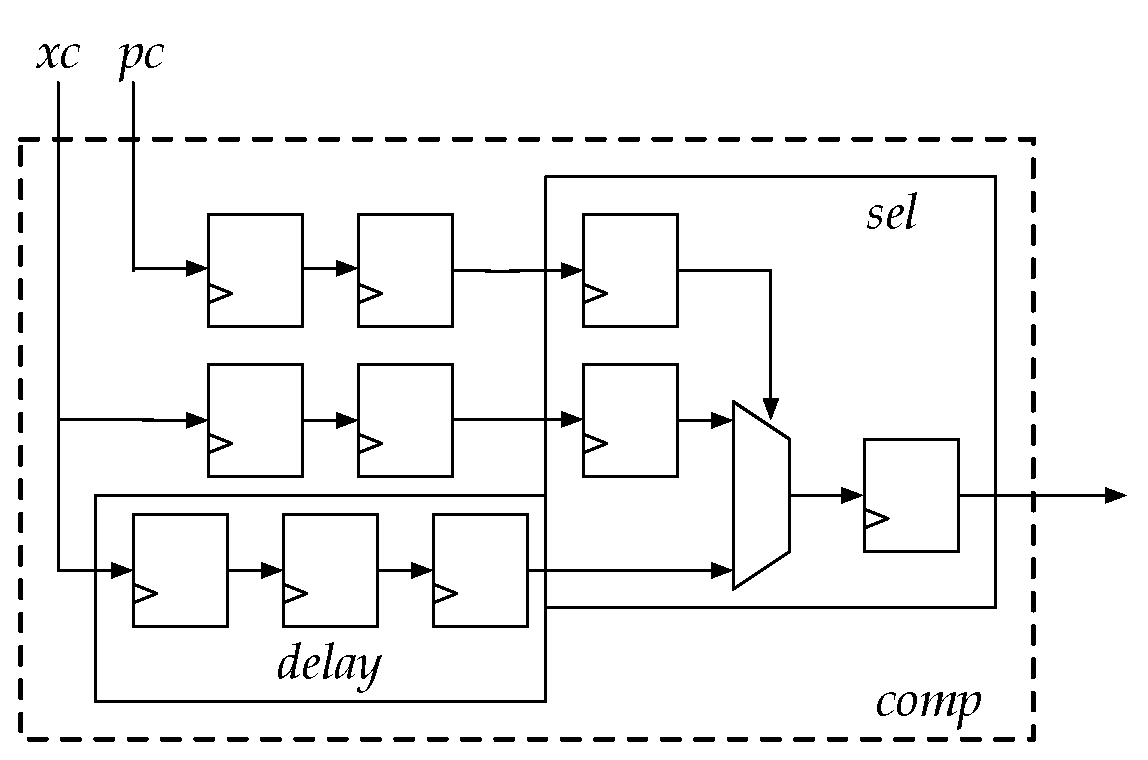
\includegraphics[width=0.8\textwidth]{images/compositionsel}
\end{center}
\caption{Composition of \ensuremath{\Varid{sel}} and \ensuremath{\Varid{delayI}} to create \ensuremath{\Varid{comp}}.} \label{fig:compositionsel}
\end{figure}


The code from code snippet \ref{code:constraintgenex1} is represented by the \gls{ast} of code snippet \ref{code:constraintgenex2}.
The term \ensuremath{\Varid{comp}} is passed to the \ensuremath{\Varid{contraints}} function as explained in the previous section.

\begin{texexptitled}[text only]{Example of constraint generation (2).}{code:constraintgenex2}
\begin{hscode}\SaveRestoreHook
\column{B}{@{}>{\hspre}l<{\hspost}@{}}%
\column{9}{@{}>{\hspre}l<{\hspost}@{}}%
\column{11}{@{}>{\hspre}l<{\hspost}@{}}%
\column{15}{@{}>{\hspre}l<{\hspost}@{}}%
\column{17}{@{}>{\hspre}l<{\hspost}@{}}%
\column{23}{@{}>{\hspre}l<{\hspost}@{}}%
\column{25}{@{}>{\hspre}l<{\hspost}@{}}%
\column{E}{@{}>{\hspre}l<{\hspost}@{}}%
\>[B]{}\Varid{delayI}\mathrel{=}{}\<[11]%
\>[11]{}\Conid{TmTAbs}\;\text{\tt \char34 t0\char34}\mathbin{\$}{}\<[E]%
\\
\>[11]{}\Conid{TmAs}\;{}\<[17]%
\>[17]{}(\Conid{TmAbs}\;\text{\tt \char34 xd\char34}\;(\Conid{TmVar}\;\mathrm{0}))\mathbin{\$}{}\<[E]%
\\
\>[17]{}\Conid{Arrow}\;{}\<[25]%
\>[25]{}(\Conid{Constant}\mathbin{\$}\Conid{TimedType}\;\Conid{TyInt}\;(\Conid{TimeExpr}\;\mathrm{0}\;\mathrm{0}))\;{}\<[E]%
\\
\>[25]{}(\Conid{Constant}\mathbin{\$}\Conid{TimedType}\;\Conid{TyInt}\;(\Conid{TimeExpr}\;\mathrm{0}\;\mathrm{3})){}\<[E]%
\\[\blanklineskip]%
\>[B]{}\Varid{sel}\mathrel{=}{}\<[9]%
\>[9]{}\Conid{TmTAbs}\;\text{\tt \char34 t1\char34}\mathbin{\$}{}\<[E]%
\\
\>[9]{}\Conid{TmAs}\;{}\<[15]%
\>[15]{}(\Conid{TmAbs}\;\text{\tt \char34 p\char34}\mathbin{\$}\Conid{TmAbs}\;\text{\tt \char34 x\char34}\mathbin{\$}\Conid{TmAbs}\;\text{\tt \char34 y\char34}\mathbin{\$}{}\<[E]%
\\
\>[15]{}(\Conid{TmIf}\;(\Conid{TmVar}\;\mathrm{2})\;(\Conid{TmVar}\;\mathrm{1})\;(\Conid{TmVar}\;\mathrm{0})))\;{}\<[E]%
\\
\>[15]{}(\Conid{Arrow}\;{}\<[23]%
\>[23]{}(\Conid{Constant}\mathbin{\$}\Conid{TimedType}\;\Conid{TyBool}\;(\Conid{TimeExpr}\;\mathrm{0}\;\mathrm{0})){}\<[E]%
\\
\>[15]{}(\Conid{Arrow}\;{}\<[23]%
\>[23]{}(\Conid{Constant}\mathbin{\$}\Conid{TimedType}\;\Conid{TyInt}\;(\Conid{TimeExpr}\;\mathrm{0}\;\mathrm{0})){}\<[E]%
\\
\>[15]{}(\Conid{Arrow}\;{}\<[23]%
\>[23]{}(\Conid{Constant}\mathbin{\$}\Conid{TimedType}\;\Conid{TyInt}\;(\Conid{TimeExpr}\;\mathrm{0}\;\mathrm{1}))\;{}\<[E]%
\\
\>[23]{}(\Conid{Constant}\mathbin{\$}\Conid{TimedType}\;\Conid{TyInt}\;(\Conid{TimeExpr}\;\mathrm{0}\;\mathrm{2}))))){}\<[E]%
\\[\blanklineskip]%
\>[B]{}\Varid{comp}\mathrel{=}{}\<[9]%
\>[9]{}\Conid{TmAbs}\;\text{\tt \char34 pc\char34}\mathbin{\$}\Conid{TmAbs}\;\text{\tt \char34 xc\char34}\mathbin{\$}{}\<[E]%
\\
\>[9]{}\Conid{TmApp}\;{}\<[17]%
\>[17]{}(\Conid{TmApp}\;{}\<[25]%
\>[25]{}(\Conid{TmApp}\;\Varid{sel}\;(\Conid{TmVar}\;\mathrm{1}))\;{}\<[E]%
\\
\>[25]{}(\Conid{TmVar}\;\mathrm{0}))\;{}\<[E]%
\\
\>[17]{}(\Conid{TmApp}\;\Varid{delayI}\;(\Conid{TmVar}\;\mathrm{0})){}\<[E]%
\ColumnHook
\end{hscode}\resethooks
\end{texexptitled}

The constraints which are generated by the constraint generation algorithm include many type variables.
We choose to represent type variables by \ensuremath{\Conid{Xn}}, where \ensuremath{\Varid{n}} is the unique identifier for the type variable.
Similarly, we choose to represent the time variables by \ensuremath{\Varid{tn}}.
The constraints generated by the algorithm for \ensuremath{\Varid{comp}} are the following:
\begin{changemargin}{1cm}{0cm}
\begin{expansionno}{text only}
\begin{tabular}{l l}
\ensuremath{\Conid{X1}\mathrel{=}\Conid{X0}\to \Conid{X3}}   &   \ensuremath{\Conid{X3}\mathrel{=}\Conid{X2}\to \Conid{X15}} \\
\ensuremath{\Conid{X7}\mathrel{=}\Conid{Bool}\langle\Varid{t2}\rangle}   &   \ensuremath{\Conid{X13}\mathrel{=}\Conid{X2}\to \Conid{X14}} \\
\ensuremath{\Conid{X8}\mathrel{=}\Conid{X0}\to \Conid{X13}}  &   \ensuremath{\Conid{X8}\mathrel{=}\Conid{Bool}\langle\Varid{t1}\mathbin{+}\mathrm{0}\rangle\to \Conid{Int}\langle\Varid{t1}\mathbin{+}\mathrm{0}\rangle} \\ 
                  &   $\quad\:$ \ensuremath{\to \Conid{Int}\langle\Varid{t1}\mathbin{+}\mathrm{1}\rangle\to \Conid{Int}\langle\Varid{t1}\mathbin{+}\mathrm{2}\rangle} \\
\ensuremath{\Conid{X8}\mathrel{=}\Conid{X7}\to \Conid{X10}}  &   \ensuremath{\Conid{X10}\mathrel{=}\Conid{X9}\to \Conid{X12}} \\
\ensuremath{\Conid{X5}\mathrel{=}\Conid{X2}\to \Conid{X6}}   &   \ensuremath{\Conid{X14}\mathrel{=}\Conid{X6}\to \Conid{X15}}\\
\ensuremath{\Conid{X9}\mathrel{=}\Conid{X11}}        &   \ensuremath{\Conid{X12}\mathrel{=}\Conid{X11}\to \Conid{X9}}\\
\ensuremath{\Conid{X5}\mathrel{=}\Conid{X4}\to \Conid{X4}}   &   \ensuremath{\Conid{X5}\mathrel{=}\Conid{Int}\langle\Varid{t0}\rangle\to \Conid{Int}\langle\Varid{t0}\mathbin{+}\mathrm{3}\rangle}\\
\end{tabular}
\end{expansionno}
\end{changemargin}

As shown, the ascription introduces the constraints \ensuremath{\Conid{X8}\mathrel{=}\Conid{Bool}\langle\Varid{t1}\mathbin{+}\mathrm{0}\rangle\to \Conid{Int}\langle\Varid{t1}\mathbin{+}\mathrm{0}\rangle\to \Conid{Int}\langle\Varid{t1}\mathbin{+}\mathrm{1}\rangle\to \Conid{Int}\langle\Varid{t1}\mathbin{+}\mathrm{2}\rangle} and \ensuremath{\Conid{X5}\mathrel{=}\Conid{Int}\langle\Varid{t0}\rangle\to \Conid{Int}\langle\Varid{t0}\mathbin{+}\mathrm{3}\rangle} for \ensuremath{\Varid{sel}} and \ensuremath{\Varid{delayI}} respectively.
The constraint \ensuremath{\Conid{X7}\mathrel{=}\Conid{Bool}\langle\Varid{t2}\rangle} is introduced by the \ensuremath{\Conid{TmIf}} rule.
To provide a mapping between type variables and types, we must unify the constraints, which we discuss in the next section.

\section{Unification}
We chose to implement a single unification algorithm, which is flexible enough to allow unification of time expressions, as well as unification of base types.
The similarities between both forms of unification are big enough to warrant a flexible definition.
Moreover, at the point of creating the implementation, the method of checking the time expressions was still in development.
As such, a flexible form of unification helped with development, as it allows us to easily modify the unification algorithm.
The unification algorithm is shown by code snippet \ref{code:unification}.
Before applying \ensuremath{\Varid{unify}} to the set of constraints, the constraints are split in a base type part, as well as a part which only contains time expressions.
The unification algorithm only works on constraints which are instances of the \ensuremath{\Conid{Substitutable}} typeclass, shown by code snippet \ref{code:substitutable}.

\begin{texexptitled}[text only]{Substitutable typeclass}{code:substitutable}
\begin{hscode}\SaveRestoreHook
\column{B}{@{}>{\hspre}l<{\hspost}@{}}%
\column{5}{@{}>{\hspre}l<{\hspost}@{}}%
\column{13}{@{}>{\hspre}l<{\hspost}@{}}%
\column{E}{@{}>{\hspre}l<{\hspost}@{}}%
\>[B]{}\mathbf{class}\;\Conid{Eq}\;\Varid{a}\Rightarrow \Conid{Substitutable}\;\Varid{z}\;\Varid{a}\;\mathbf{where}{}\<[E]%
\\
\>[B]{}\hsindent{5}{}\<[5]%
\>[5]{}\Varid{add}{}\<[13]%
\>[13]{}\mathbin{::}\Conid{Substitution}\;\Varid{a}\to \Varid{z}\to \Varid{z}{}\<[E]%
\\
\>[B]{}\hsindent{5}{}\<[5]%
\>[5]{}\Varid{apply}{}\<[13]%
\>[13]{}\mathbin{::}([\mskip1.5mu \Conid{Substitution}\;\Varid{a}\mskip1.5mu]\to [\mskip1.5mu \Conid{Substitution}\;\Varid{a}\mskip1.5mu])\to \Varid{z}\to \Varid{z}{}\<[E]%
\\
\>[B]{}\hsindent{5}{}\<[5]%
\>[5]{}\Varid{match}{}\<[13]%
\>[13]{}\mathbin{::}\Varid{a}\to \Varid{a}\to \Varid{z}\to \Varid{z}{}\<[E]%
\ColumnHook
\end{hscode}\resethooks
\end{texexptitled}

\begin{texexptitled}[text only]{Unification}{code:unification}
\begin{hscode}\SaveRestoreHook
\column{B}{@{}>{\hspre}l<{\hspost}@{}}%
\column{5}{@{}>{\hspre}l<{\hspost}@{}}%
\column{9}{@{}>{\hspre}l<{\hspost}@{}}%
\column{30}{@{}>{\hspre}c<{\hspost}@{}}%
\column{30E}{@{}l@{}}%
\column{33}{@{}>{\hspre}l<{\hspost}@{}}%
\column{39}{@{}>{\hspre}l<{\hspost}@{}}%
\column{43}{@{}>{\hspre}l<{\hspost}@{}}%
\column{47}{@{}>{\hspre}l<{\hspost}@{}}%
\column{49}{@{}>{\hspre}l<{\hspost}@{}}%
\column{55}{@{}>{\hspre}l<{\hspost}@{}}%
\column{E}{@{}>{\hspre}l<{\hspost}@{}}%
\>[B]{}\Varid{unify}\mathbin{::}(\Conid{Show}\;\Varid{a},\Conid{Substitutable}\;\Varid{z}\;\Varid{a})\Rightarrow [\mskip1.5mu \Conid{Constraint}\;\Varid{a}\mskip1.5mu]\to \Varid{z}\to \Varid{z}{}\<[E]%
\\
\>[B]{}\Varid{unify}\;[\mskip1.5mu \mskip1.5mu]\;\Varid{r}\mathrel{=}\Varid{id}\;\Varid{r}{}\<[E]%
\\
\>[B]{}\Varid{unify}\;(\Varid{c}\mathbin{:}\Varid{cs})\;\Varid{r}\mathrel{=}\mathbf{case}\;\Varid{c}\;\mathbf{of}{}\<[E]%
\\
\>[B]{}\hsindent{5}{}\<[5]%
\>[5]{}(\Conid{Constant}\;\Varid{t1},\Conid{Constant}\;\Varid{t2}){}\<[33]%
\>[33]{}\to \Varid{unify}\;\Varid{cs}\mathbin{\$}\Varid{match}\;\Varid{t1}\;\Varid{t2}\;\Varid{r}{}\<[E]%
\\
\>[B]{}\hsindent{5}{}\<[5]%
\>[5]{}(\Conid{Arrow}\;\Varid{s1}\;\Varid{s2},\Conid{Arrow}\;\Varid{t1}\;\Varid{t2}){}\<[39]%
\>[39]{}\to \Varid{unify}\;((\Varid{s1},\Varid{t1})\mathbin{:}(\Varid{s2},\Varid{t2})\mathbin{:}\Varid{cs})\;\Varid{r}{}\<[E]%
\\
\>[B]{}\hsindent{5}{}\<[5]%
\>[5]{}(\Varid{tyS}\mathord{@}(\Conid{Var}\;\Varid{idS}),\Varid{tyT}{}\<[30]%
\>[30]{}){}\<[30E]%
\\
\>[5]{}\hsindent{4}{}\<[9]%
\>[9]{}\mid \Varid{tyS}\equiv \Varid{tyT}{}\<[39]%
\>[39]{}\to {}\<[43]%
\>[43]{}\Varid{unify}\;\Varid{cs}\;\Varid{r}{}\<[E]%
\\
\>[5]{}\hsindent{4}{}\<[9]%
\>[9]{}\mid \neg \mathbin{\$}\Varid{idS}\mathbin{`\Varid{isFVIn}`}\Varid{tyT}{}\<[39]%
\>[39]{}\to {}\<[43]%
\>[43]{}\mathbf{let}\;{}\<[49]%
\>[49]{}\Varid{cs'}{}\<[55]%
\>[55]{}\mathrel{=}(\Varid{tyS}\mapsto\Varid{tyT})\;\Varid{cs}{}\<[E]%
\\
\>[49]{}\Varid{r'}{}\<[55]%
\>[55]{}\mathrel{=}\Varid{add}\;(\Varid{tyS},\Varid{tyT})\mathbin{\$}\Varid{apply}\;(\Varid{tyS}\mapsto\Varid{tyT})\;\Varid{r}{}\<[E]%
\\
\>[43]{}\mathbf{in}\;{}\<[47]%
\>[47]{}\Varid{unify}\;\Varid{cs'}\;\Varid{r'}{}\<[E]%
\\[\blanklineskip]%
\>[B]{}\hsindent{5}{}\<[5]%
\>[5]{}(\Varid{tyS},\Varid{tyT}\mathord{@}(\Conid{Var}\;\Varid{idT}){}\<[30]%
\>[30]{}){}\<[30E]%
\>[39]{}\to \Varid{unify}\;((\Varid{tyT},\Varid{tyS})\mathbin{:}\Varid{cs})\;\Varid{r}{}\<[E]%
\\
\>[B]{}\hsindent{5}{}\<[5]%
\>[5]{}(\Varid{t1},\Varid{t2}{}\<[30]%
\>[30]{}){}\<[30E]%
\>[39]{}\to \Varid{error}\;\text{\tt \char34 not~unifiable~\char34}{}\<[E]%
\ColumnHook
\end{hscode}\resethooks
\end{texexptitled}

In the substitutable typeclass, \ensuremath{\Varid{a}} represents the type of constraints, which is either a base type or a time expression.
Depending on the type of constraints, a different record can be used to build the list of substitutions.
The list of substitutions provides a mapping between type variables and constant types.
The different operations of the \ensuremath{\Conid{Substitutable}} typeclass are explained when we discuss the unification algorithm.
However, we point out that these operations, together with the polymorphic container type \ensuremath{\Varid{z}}, allow us to modify the resulting substitutions by the unification algorithm.

As shown, \ensuremath{\Varid{unify}} accepts two arguments.
One is a set of constraints, the other being a record type which is defined by the \ensuremath{\Conid{Substitutable}} typeclass.
To clarify the algorithm, we first focus on how it is implemented for base types, before showing how it is implemented for time expressions.
The base type instance of the \ensuremath{\Conid{Substitutable}} typeclass is defined by code snippet \ref{code:priminstance}.

\begin{texexptitled}[text only]{BaseTypes instance}{code:priminstance}
\begin{hscode}\SaveRestoreHook
\column{B}{@{}>{\hspre}l<{\hspost}@{}}%
\column{5}{@{}>{\hspre}l<{\hspost}@{}}%
\column{9}{@{}>{\hspre}l<{\hspost}@{}}%
\column{E}{@{}>{\hspre}l<{\hspost}@{}}%
\>[B]{}\mathbf{type}\;\Conid{Substitution}\;\Varid{a}\mathrel{=}(\Conid{MetaType}\;\Varid{a},\Conid{MetaType}\;\Varid{a}){}\<[E]%
\\
\>[B]{}\mathbf{data}\;\Conid{BaseRecord}\mathrel{=}\Conid{BaseRecord}\;[\mskip1.5mu \Conid{Substitution}\;\Conid{BaseType}\mskip1.5mu]{}\<[E]%
\\[\blanklineskip]%
\>[B]{}\mathbf{instance}\;\Conid{Substitutable}\;\Conid{BaseRecord}\;\Conid{BaseType}\;\mathbf{where}{}\<[E]%
\\
\>[B]{}\hsindent{5}{}\<[5]%
\>[5]{}\Varid{add}\;\Varid{x}\;(\Conid{BaseRecord}\;\Varid{xs})\mathrel{=}\Conid{BaseRecord}\;(\Varid{x}\mathbin{:}\Varid{xs}){}\<[E]%
\\
\>[B]{}\hsindent{5}{}\<[5]%
\>[5]{}\Varid{apply}\;\Varid{f}\;(\Conid{BaseRecord}\;\Varid{xs})\mathrel{=}\Conid{BaseRecord}\mathbin{\$}\Varid{f}\;\Varid{xs}{}\<[E]%
\\
\>[B]{}\hsindent{5}{}\<[5]%
\>[5]{}\Varid{match}\;\Varid{x}\;\Varid{y}\;\Varid{tr}{}\<[E]%
\\
\>[5]{}\hsindent{4}{}\<[9]%
\>[9]{}\mid \Varid{x}\equiv \Varid{y}\mathrel{=}\Varid{tr}{}\<[E]%
\\
\>[5]{}\hsindent{4}{}\<[9]%
\>[9]{}\mid \Varid{otherwise}\mathrel{=}\Varid{error}\;\text{\tt \char34 x~/=~y\char34}{}\<[E]%
\ColumnHook
\end{hscode}\resethooks
\end{texexptitled}

The \ensuremath{\Varid{unify}} function has five distinct cases of constraints which are handled.
First, the constraint between two constant types are compared.
For this, the \ensuremath{\Varid{match}} function is used, which is part of the \ensuremath{\Conid{Substitutable}} typeclass. 
The functionality of \ensuremath{\Varid{match}} depends on the type of constraints which are unified.
In the case of base types, \ensuremath{\Varid{match}} just checks for equality.
When base types are not equal, an error is raised to indicate that the checked term is not well-typed.

The second case of \ensuremath{\Varid{unify}} handles function constraints, where a function type is constrained by another function type. 
When a function type is constrained by a non-function type, then the term is not well-typed.
If it is constrained by another function type, the individual types which make up the function types are \textit{added} to the existing set of constraints.

The third case of \ensuremath{\Varid{unify}} matches a type variable $X_{idS}$ to an unknown type \ensuremath{\Varid{tyT}}.
If the left hand side of the constraint is equal to the right hand side, then the constraint is discarded and unification continues for the remaining constraints.
If they are not the same, then it is checked whether or not the type variable $X_{idS}$ exists as a free type variable within $tyT$.
Checking for free type variables are important.  
Consider the constraint \ensuremath{\Conid{X0}\mathrel{=}\Conid{X1}\to \Conid{X0}}, where \ensuremath{\Conid{X0}} is not free in \ensuremath{\Conid{X1}\to \Conid{X0}}.
This constraint is not well-typed, as we do not support recursion.

If this is not the case, then the variable $X_{idS}$ is replaced by \ensuremath{\Varid{tyT}} in the remaining constraints, as indicated by the \ensuremath{(\mapsto)} function.
Since we have made a substitution in the form of $X_{idS} \mapsto tyT$, we store the substitution.
However, aside from applying the substitution to the remaining constraints, the substitution is also applied to the existing substitutions, which is what the \ensuremath{\Varid{apply}} function does in the case of base types.
The way existing substutions are stored depends on the type of constraints which are being unified.
As a result, the functions \ensuremath{\Varid{add}} and \ensuremath{\Varid{apply}} are part of the \ensuremath{\Conid{Substitutable}} typeclass.
In the case of base types, substitutions are added to the record, while existing substitutions within the record are rewritten according to the new substitution.
The fourth case of \ensuremath{\Varid{unify}} is the same as the third case, only with the right hand side and left hand side switched. 
Finally, the fifth case represents the case when terms are not well-typed.

\begin{texexptitled}[text only]{\ensuremath{\Conid{TimeExpr}} instance of \ensuremath{\Conid{Substitutable}}}{code:timeinstance}
\begin{hscode}\SaveRestoreHook
\column{B}{@{}>{\hspre}l<{\hspost}@{}}%
\column{5}{@{}>{\hspre}l<{\hspost}@{}}%
\column{7}{@{}>{\hspre}l<{\hspost}@{}}%
\column{12}{@{}>{\hspre}l<{\hspost}@{}}%
\column{17}{@{}>{\hspre}l<{\hspost}@{}}%
\column{E}{@{}>{\hspre}l<{\hspost}@{}}%
\>[B]{}\mathbf{data}\;\Conid{TimeRecord}\mathrel{=}\Conid{TimeRecord}{}\<[E]%
\\
\>[B]{}\hsindent{17}{}\<[17]%
\>[17]{}\{\mskip1.5mu \Varid{timeSubs}\mathbin{::}[\mskip1.5mu \Conid{Substitution}\;\Conid{TimeExpr}\mskip1.5mu]{}\<[E]%
\\
\>[B]{}\hsindent{17}{}\<[17]%
\>[17]{},\Varid{timeVars}\mathbin{::}[\mskip1.5mu (\Conid{TimeExpr},\Conid{TimeExpr})\mskip1.5mu]\mskip1.5mu\}{}\<[E]%
\\[\blanklineskip]%
\>[B]{}\mathbf{instance}\;\Conid{Substitutable}\;\Conid{TimeRecord}\;\Conid{TimeExpr}\;\mathbf{where}{}\<[E]%
\\
\>[B]{}\hsindent{5}{}\<[5]%
\>[5]{}\Varid{add}\;\Varid{x}\;\Varid{tr}\mathrel{=}\Varid{tr}\;\{\mskip1.5mu \Varid{timeSubs}\mathrel{=}\Varid{x}\mathbin{:}(\Varid{timeSubs}\;\Varid{tr})\mskip1.5mu\}{}\<[E]%
\\
\>[B]{}\hsindent{5}{}\<[5]%
\>[5]{}\Varid{apply}\;\Varid{f}\;\Varid{tr}\mathrel{=}\Varid{tr}\;\{\mskip1.5mu \Varid{timeSubs}\mathrel{=}\Varid{f}\mathbin{\$}\Varid{timeSubs}\;\Varid{tr}\mskip1.5mu\}{}\<[E]%
\\
\>[B]{}\hsindent{5}{}\<[5]%
\>[5]{}\Varid{match}\;\Varid{x}\;\Varid{y}\;\Varid{tr}\mathrel{=}{}\<[E]%
\\
\>[5]{}\hsindent{2}{}\<[7]%
\>[7]{}\mathbf{let}\;\Varid{maysub}\mathrel{=}\Varid{matchConstantType}\;(\Varid{x},\Varid{y}){}\<[E]%
\\
\>[5]{}\hsindent{2}{}\<[7]%
\>[7]{}\mathbf{in}\;\mathbf{case}\;\Varid{maysub}\;\mathbf{of}{}\<[E]%
\\
\>[7]{}\hsindent{5}{}\<[12]%
\>[12]{}\Conid{Just}\;\Varid{z}\to \Varid{tr}\;\{\mskip1.5mu \Varid{timeVars}\mathrel{=}\Varid{z}\mathbin{:}(\Varid{timeVars}\;\Varid{tr})\mskip1.5mu\}{}\<[E]%
\\
\>[7]{}\hsindent{5}{}\<[12]%
\>[12]{}\Conid{Nothing}\to \Varid{tr}{}\<[E]%
\ColumnHook
\end{hscode}\resethooks
\end{texexptitled}

The same algorithm is used for time expressions. 
The code of snippet \ref{code:timeinstance} shows the \ensuremath{\Conid{TimeExpr}} instance of \ensuremath{\Conid{Substitutable}}.
The unification algorithm uses \ensuremath{\Conid{TimeRecord}} to store substitutions.
The \ensuremath{\Varid{timeSubs}} stores the substitutions, while \ensuremath{\Varid{timeVars}} is used to verify time expressions.
To create substitutions, first the unification algorithm finds the relations between time expressions which are needed to verify the time-dependent behaviour.
These relations are stored in \ensuremath{\Varid{timeVars}}.
After the time-expressions are verified, the \textit{original} set of constraints is modified.
The resulting constraints are then unified \textit{again}, after which \ensuremath{\Varid{timeSubs}} contains the final substitutions.
Adding the substitutions and applying them to time variables is straightforward.
However, matching time expressions is more complex, as shown by code snippet \ref{code:timematch}.
The result of \ensuremath{\Varid{matchConstantType}} are added to \ensuremath{\Varid{timeVars}}, which is used to verify the time expressions.

\begin{texexptitled}[text only]{Matching function for time expressions}{code:timematch}
\begin{hscode}\SaveRestoreHook
\column{B}{@{}>{\hspre}l<{\hspost}@{}}%
\column{3}{@{}>{\hspre}l<{\hspost}@{}}%
\column{5}{@{}>{\hspre}l<{\hspost}@{}}%
\column{7}{@{}>{\hspre}l<{\hspost}@{}}%
\column{21}{@{}>{\hspre}l<{\hspost}@{}}%
\column{25}{@{}>{\hspre}l<{\hspost}@{}}%
\column{E}{@{}>{\hspre}l<{\hspost}@{}}%
\>[B]{}\Varid{matchConstantType}\;\Varid{c}\mathrel{=}{}\<[E]%
\\
\>[B]{}\hsindent{3}{}\<[3]%
\>[3]{}\mathbf{case}\;\Varid{c}\;\mathbf{of}{}\<[E]%
\\
\>[3]{}\hsindent{2}{}\<[5]%
\>[5]{}(\Conid{TimeExpr}\;\Varid{t1}\;\Varid{o1},\Conid{TimeExpr}\;\Varid{t2}\;\Varid{o2}){}\<[E]%
\\
\>[5]{}\hsindent{2}{}\<[7]%
\>[7]{}\mid \Varid{t1}\equiv \Varid{t2}{}\<[21]%
\>[21]{}\to {}\<[25]%
\>[25]{}\Conid{Nothing}{}\<[E]%
\\
\>[5]{}\hsindent{2}{}\<[7]%
\>[7]{}\mid \Varid{otherwise}{}\<[21]%
\>[21]{}\to {}\<[25]%
\>[25]{}\Conid{Just}\;(\Conid{TimeExpr}\;\Varid{t1}\;\Varid{o1},\Conid{TimeExpr}\;\Varid{t2}\;\Varid{o2}){}\<[E]%
\\[\blanklineskip]%
\>[3]{}\hsindent{2}{}\<[5]%
\>[5]{}(\Conid{TimeLiteral}\;\Varid{o1},\Conid{TimeLiteral}\;\Varid{o2}){}\<[E]%
\\
\>[5]{}\hsindent{2}{}\<[7]%
\>[7]{}\mid \Varid{o1}\equiv \Varid{o2}{}\<[21]%
\>[21]{}\to {}\<[25]%
\>[25]{}\Conid{Nothing}{}\<[E]%
\\
\>[5]{}\hsindent{2}{}\<[7]%
\>[7]{}\mid \Varid{otherwise}{}\<[21]%
\>[21]{}\to {}\<[25]%
\>[25]{}\Varid{error}\;\text{\tt \char34 cannot~unify~literals~o1~o2\char34}{}\<[E]%
\\[\blanklineskip]%
\>[3]{}\hsindent{2}{}\<[5]%
\>[5]{}(\Varid{c1}\mathord{@}(\Conid{TimeExpr}\;\Varid{t1}\;\Varid{o1}),\Varid{c2}\mathord{@}(\Conid{TimeLiteral}\;\Varid{o2})){}\<[E]%
\\
\>[5]{}\hsindent{16}{}\<[21]%
\>[21]{}\to {}\<[25]%
\>[25]{}\Conid{Just}\;(\Varid{c2},\Varid{c1}){}\<[E]%
\\[\blanklineskip]%
\>[3]{}\hsindent{2}{}\<[5]%
\>[5]{}(\Varid{c1}\mathord{@}(\Conid{TimeLiteral}\;\Varid{o1}),\Varid{c2}\mathord{@}(\Conid{TimeExpr}\;\Varid{t2}\;\Varid{o2})){}\<[E]%
\\
\>[5]{}\hsindent{16}{}\<[21]%
\>[21]{}\to \Varid{matchConstantType}\;\Varid{c2}\;\Varid{c1}{}\<[E]%
\ColumnHook
\end{hscode}\resethooks
\end{texexptitled}

When matching time expressions, four different cases can be distinguished.
Either a time expression is constrained to another time expression, a literal is constrained to another literal, a literal is constrained by a time expression, or vice versa.
The first case filters the time expressions which are needed to verify the time-dependent behaviour.
For instance, when typechecking the function \ensuremath{\Varid{f}\;\Varid{x}\;\Varid{y}\mathrel{=}\Varid{y}} with type \ensuremath{\Conid{Bool}\langle\Varid{t}\rangle\to \Conid{Bool}\langle\Varid{t}\mathbin{+}\mathrm{1}\rangle\to \Conid{Bool}\langle\Varid{t}\mathbin{+}\mathrm{2}\rangle}, the result would be the equality of \ensuremath{\Conid{Bool}\langle\Varid{t}\mathbin{+}\mathrm{1}\rangle\mathrel{=}\Conid{Bool}\langle\Varid{t}\mathbin{+}\mathrm{2}\rangle}.
This equality is created as \ensuremath{\Varid{y}} on the left hand side of the expression has type \ensuremath{\Conid{Bool}\langle\Varid{t}\mathbin{+}\mathrm{1}\rangle}, while \ensuremath{\Varid{y}} on the right hand side of the expressions has type \ensuremath{\Conid{Bool}\langle\Varid{t}\mathbin{+}\mathrm{2}\rangle}.
Since these time variables are the same, we can determine that this is indeed allowed, as function definitions can only have \textit{increasing} delays.
However, in a constraint with different time variables, such as \ensuremath{\Conid{Bool}\langle\Varid{t0}\mathbin{+}\mathrm{1}\rangle\mathrel{=}\Conid{Bool}\langle\Varid{t1}\mathbin{+}\mathrm{2}\rangle}, we cannot determine if this is actually allowed behaviour.
For the purpose of checking the time constraints at a later point, the constraint is recorded and added to \ensuremath{\Varid{timeVars}}, as shown by code snippet \ref{code:timeinstance}.

The second case of \ensuremath{\Varid{matchConstantType}} checks literals. 
In the prototype typechecker, these literals are only compared for equality.
For the purpose of showing that the principle of checking time expressions actually work this is enough, though it could be extended to allow delays on values which exist at a specific time.

The last two cases of \ensuremath{\Varid{matchConstantType}} check time expressions which are constrained to literals, and vice versa.
When time expressions are constrained to literals, the constraint is added with the left hand side containing the literal, and the right hand side containing the time expression.

\subsection{Example of Unification}
Given the constraints generated earlier, repeated below for convenience, we unify them.
We only show the full unification of base types here.
To show unification of time expressions, we first need to generate the time variables which are checked seperately.

\begin{changemargin}{1cm}{0cm}
\begin{expansionno}{text only}
\begin{tabular}{l l}
\ensuremath{\Conid{X1}\mathrel{=}\Conid{X0}\to \Conid{X3}}   &   \ensuremath{\Conid{X3}\mathrel{=}\Conid{X2}\to \Conid{X15}} \\
\ensuremath{\Conid{X7}\mathrel{=}\Conid{Bool}\langle\Varid{t2}\rangle}   &   \ensuremath{\Conid{X13}\mathrel{=}\Conid{X2}\to \Conid{X14}} \\
\ensuremath{\Conid{X8}\mathrel{=}\Conid{X0}\to \Conid{X13}}  &   \ensuremath{\Conid{X8}\mathrel{=}\Conid{Bool}\langle\Varid{t1}\mathbin{+}\mathrm{0}\rangle\to \Conid{Int}\langle\Varid{t1}\mathbin{+}\mathrm{0}\rangle} \\ 
                  &   $\quad\:$ \ensuremath{\to \Conid{Int}\langle\Varid{t1}\mathbin{+}\mathrm{1}\rangle\to \Conid{Int}\langle\Varid{t1}\mathbin{+}\mathrm{2}\rangle} \\
\ensuremath{\Conid{X8}\mathrel{=}\Conid{X7}\to \Conid{X10}}  &   \ensuremath{\Conid{X10}\mathrel{=}\Conid{X9}\to \Conid{X12}} \\
\ensuremath{\Conid{X5}\mathrel{=}\Conid{X2}\to \Conid{X6}}   &   \ensuremath{\Conid{X14}\mathrel{=}\Conid{X6}\to \Conid{X15}}\\
\ensuremath{\Conid{X9}\mathrel{=}\Conid{X11}}        &   \ensuremath{\Conid{X12}\mathrel{=}\Conid{X11}\to \Conid{X9}}\\
\ensuremath{\Conid{X5}\mathrel{=}\Conid{X4}\to \Conid{X4}}   &   \ensuremath{\Conid{X5}\mathrel{=}\Conid{Int}\langle\Varid{t0}\rangle\to \Conid{Int}\langle\Varid{t0}\mathbin{+}\mathrm{10}\rangle}\\
\end{tabular}
\end{expansionno}
\end{changemargin}

After splitting these constraints into base types and time expressions, we can pass them to the unification algorithm.
In the case of base types, the resulting mapping is 
\begin{changemargin}{1cm}{0cm}
\begin{expansionno}{text only}
\begin{tabular}{l l}
\ensuremath{\Conid{X0}\mathrel{=}\Conid{Bool}}               & \ensuremath{\Conid{X1}\mathrel{=}\Conid{Bool}\to \Conid{Int}\to \Conid{Int}} \\
\ensuremath{\Conid{X2}\mathrel{=}\Conid{Int}}                & \ensuremath{\Conid{X3}\mathrel{=}\Conid{Int}\to \Conid{Int}}\\
\ensuremath{\Conid{X4}\mathrel{=}\Conid{Int}}                & \ensuremath{\Conid{X5}\mathrel{=}\Conid{Int}\to \Conid{Int}}\\
\ensuremath{\Conid{X6}\mathrel{=}\Conid{Int}}                & \ensuremath{\Conid{X7}\mathrel{=}\Conid{Bool}}\\
\ensuremath{\Conid{X8}\mathrel{=}\Conid{Bool}\to \Conid{Int}\to \Conid{Int}\to \Conid{Int}} & \ensuremath{\Conid{X9}\mathrel{=}\Conid{Int}}\\
\ensuremath{\Conid{X10}\mathrel{=}\Conid{Int}\to \Conid{Int}\to \Conid{Int}} & \ensuremath{\Conid{X11}\mathrel{=}\Conid{Int}}\\
\ensuremath{\Conid{X12}\mathrel{=}\Conid{Int}\to \Conid{Int}}        & \ensuremath{\Conid{X13}\mathrel{=}\Conid{Int}\to \Conid{Int}\to \Conid{Int}}\\ 
\ensuremath{\Conid{X14}\mathrel{=}\Conid{Int}\to \Conid{Int}}        & \ensuremath{\Conid{X15}\mathrel{=}\Conid{Int}}
\end{tabular}
\end{expansionno}
\end{changemargin}
The constraint generation algorithm defined the type of \ensuremath{\Varid{comp}} to be equal to \ensuremath{\Conid{X1}}.
As shown, the resulting type of \ensuremath{\Varid{comp}} is \ensuremath{\Conid{Bool}\to \Conid{Int}\to \Conid{Int}}, which is as expected.
The remainder of the constraints define the types of each intermediate expression which makes up \ensuremath{\Varid{comp}}.
Given these types, we can reason about the types of every (partial) function and other values.

For time variables this is slightly different, as we have not checked whether time expressions are actually correct yet.
However, \ensuremath{\Varid{timeVars}} result in a list of constraints, which are shown below.
\begin{changemargin}{1cm}{0cm}
\begin{expansionno}{text only}
\begin{tabular}{c}
\ensuremath{\langle\Varid{t1}\mathbin{+}\mathrm{1}\rangle\mathrel{=}\langle\Varid{t0}\mathbin{+}\mathrm{3}\rangle} \\
\ensuremath{\langle\Varid{t1}\rangle\mathrel{=}\langle\Varid{t0}\rangle} \\
\ensuremath{\langle\Varid{t2}\rangle\mathrel{=}\langle\Varid{t1}\rangle} \\
\end{tabular}
\end{expansionno}
\end{changemargin}

These constraints are used to verify the complete time-dependent behaviour of \ensuremath{\Varid{comp}}, and provide placement information for memory elements.
In the next section we will use the constraints listed above.

\section{Checking Time Constraints}
Multiple methods could be used to verify the time-dependent behaviour using the constraints of \ensuremath{\Varid{timeVars}}.
We chose to use first order logic to express the constrained time expressions, and use \gls{smt} solvers to find integer representations for the time variables used in time expressions.
Using the integer representations for time variables we can then rewrite the time expressions of compositions in terms of a single time variable and its offsets. 

We chose to use the Z3\cite{de2008z3} solver, as it is the only \gls{smt} solver which supports unbounded integers.
A complete discussion about \gls{smt} solvers is out of the scope of this thesis.
However, \citeauthor{de2008z3} define \gls{smt} as follows: ``A \gls{smt} problem is a decision problem for logical first order formulas with respect to combinations of background theories such as: arithmetic, bit-vectors, arrays, and uninterpreted functions.``

Since the Z3 solver is not written in Haskell, we use the library \ensuremath{\Conid{\Conid{Data}.SBV}}\cite{sbv} to handle the interfacing with Z3.
\ensuremath{\Conid{\Conid{Data}.SBV}} provides the Haskell language with the \ensuremath{\Conid{Symbolic}} monad, which allows us to create statements in first order logic.
The library then allows us to use the Z3 solver to find integer representations for time variables.
The usage of \gls{smt} solvers in Haskell or other functional languages is not new.
Liquid Types\cite{rondon2008liquid} for instance are used to extend Hindley-Milner type inference using \gls{smt}-solvers.

As an example, we use the constrained time expressions from the previous section to create a statement in first order logic, which is checked by the Z3 solver.
\begin{changemargin}{1cm}{0cm}
\begin{expansionno}{text only}
\begin{tabular}{c}
\ensuremath{\langle\Varid{t1}\mathbin{+}\mathrm{1}\rangle\mathrel{=}\langle\Varid{t0}\mathbin{+}\mathrm{3}\rangle} \\
\ensuremath{\langle\Varid{t1}\rangle\mathrel{=}\langle\Varid{t0}\rangle} \\
\ensuremath{\langle\Varid{t2}\rangle\mathrel{=}\langle\Varid{t1}\rangle} \\
\end{tabular}
\end{expansionno}
\end{changemargin}

First, the proper ordering is determined.
Since time variables are created in order, we know that the time variable \ensuremath{\Varid{t1}} must occur later than \ensuremath{\Varid{t0}}.
Similarly, \ensuremath{\Varid{t2}} must occur later than \ensuremath{\Varid{t1}}.
Using the constrained time expressions from above, we can then define the following statement using first order logic:
\[
  \begin{array}{l l}
    \exists t0. \exists t1. \exists t2. & t1 + 1 \geq t0 + 3\\
                                        & t1 \geq t0 \\
                                        & t2 \geq t1\\
                                        & t0 \geq 0\\
                                        & t1 \geq 0\\
                                        & t2 \geq 0
  \end{array}
  \]

We create this statement by using the \ensuremath{\Conid{\Conid{Data}.SBV}} library, and ask Z3 to find integer representations for \ensuremath{\Varid{t0}}, \ensuremath{\Varid{t1}} and \ensuremath{\Varid{t2}}.
We do this by using the \ensuremath{\Conid{Symbolic}} monad, as shown by code snippet \ref{code:symbolic}.

\begin{texexptitled}[text only]{Using the \ensuremath{\Conid{Symbolic}} monad to create statements in first order logic.}{code:symbolic}
\begin{hscode}\SaveRestoreHook
\column{B}{@{}>{\hspre}l<{\hspost}@{}}%
\column{3}{@{}>{\hspre}l<{\hspost}@{}}%
\column{7}{@{}>{\hspre}l<{\hspost}@{}}%
\column{27}{@{}>{\hspre}l<{\hspost}@{}}%
\column{E}{@{}>{\hspre}l<{\hspost}@{}}%
\>[B]{}\Varid{representation}\mathrel{=}{}\<[E]%
\\
\>[B]{}\hsindent{3}{}\<[3]%
\>[3]{}\mathbf{do}\;{}\<[7]%
\>[7]{}\Varid{t1}\leftarrow\Varid{exists}\;\text{\tt \char34 t0\char34}{}\<[E]%
\\
\>[7]{}\Varid{t2}\leftarrow\Varid{exists}\;\text{\tt \char34 t1\char34}{}\<[E]%
\\
\>[7]{}\Varid{t3}\leftarrow\Varid{exists}\;\text{\tt \char34 t2\char34}{}\<[E]%
\\
\>[7]{}\Varid{constrain}\mathbin{\$}\Varid{t0}{}\<[27]%
\>[27]{}.\geq\mathrm{0}{}\<[E]%
\\
\>[7]{}\Varid{constrain}\mathbin{\$}\Varid{t1}{}\<[27]%
\>[27]{}.\geq\mathrm{0}{}\<[E]%
\\
\>[7]{}\Varid{constrain}\mathbin{\$}\Varid{t2}{}\<[27]%
\>[27]{}.\geq\mathrm{0}{}\<[E]%
\\
\>[7]{}\Varid{constrain}\mathbin{\$}\Varid{t1}\mathbin{+}\mathrm{1}{}\<[27]%
\>[27]{}.\geq\Varid{t0}\mathbin{+}\mathrm{3}{}\<[E]%
\\
\>[7]{}\Varid{constrain}\mathbin{\$}\Varid{t1}{}\<[27]%
\>[27]{}.\geq\Varid{t0}{}\<[E]%
\\
\>[7]{}\Varid{constrain}\mathbin{\$}\Varid{t2}{}\<[27]%
\>[27]{}.\geq\Varid{t1}{}\<[E]%
\\
\>[7]{}\Varid{solve}\;[\mskip1.5mu \mskip1.5mu]{}\<[E]%
\ColumnHook
\end{hscode}\resethooks
\end{texexptitled}

Using the definition of \ensuremath{\Varid{representation}}, we use the \ensuremath{\Varid{sat}} function of \ensuremath{\Conid{\Conid{Data}.SBV}} to ask the Z3 solver to find a integer representation of \ensuremath{\Varid{t0}}, \ensuremath{\Varid{t1}} and \ensuremath{\Varid{t2}}.
In our experience, Z3 automatically finds the minimal integer values, though this is not guaranteed.
In the future, Z3 will also support optimization criteria, allowing us to guarantee the minimal integer values for time variables.
If the time expressions are erroneous, the \ensuremath{\Varid{sat}} function will not return integer representations for \ensuremath{\Varid{t0}}, \ensuremath{\Varid{t1}} and \ensuremath{\Varid{t2}}.

In the case of verifying the behaviour of \ensuremath{\Varid{comp}} however, the \ensuremath{\Varid{sat}} function provides the following integer representations:
\begin{changemargin}{1cm}{0cm}
\begin{expansionno}{text only}
\ensuremath{\Varid{t0}\mathrel{=}\mathrm{0}}\\
\ensuremath{\Varid{t1}\mathrel{=}\mathrm{2}}\\
\ensuremath{\Varid{t2}\mathrel{=}\mathrm{2}}\\
\end{expansionno}
\end{changemargin}

When we assume \ensuremath{\Varid{t}\mathrel{=}\mathrm{0}}, we can rewrite the existing expressions of the original constraints as follows:

\begin{changemargin}{1cm}{0cm}
\begin{expansionno}{text only}
\begin{tabular}{l l}
\ensuremath{\Conid{X1}\mathrel{=}\Conid{X0}\to \Conid{X3}}   &   \ensuremath{\Conid{X3}\mathrel{=}\Conid{X2}\to \Conid{X15}} \\
\ensuremath{\Conid{X7}\mathrel{=}\Conid{Bool}\langle\Varid{t}\mathbin{+}\mathrm{2}\rangle}   &   \ensuremath{\Conid{X13}\mathrel{=}\Conid{X2}\to \Conid{X14}} \\
\ensuremath{\Conid{X8}\mathrel{=}\Conid{X0}\to \Conid{X13}}  &   \ensuremath{\Conid{X8}\mathrel{=}\Conid{Bool}\langle\Varid{t}\mathbin{+}\mathrm{2}\rangle\to \Conid{Int}\langle\Varid{t}\mathbin{+}\mathrm{2}\rangle} \\ 
                  &   $\quad\:$ \ensuremath{\to \Conid{Int}\langle\Varid{t}\mathbin{+}\mathrm{3}\rangle\to \Conid{Int}\langle\Varid{t}\mathbin{+}\mathrm{4}\rangle} \\
\ensuremath{\Conid{X8}\mathrel{=}\Conid{X7}\to \Conid{X10}}  &   \ensuremath{\Conid{X10}\mathrel{=}\Conid{X9}\to \Conid{X12}} \\
\ensuremath{\Conid{X5}\mathrel{=}\Conid{X2}\to \Conid{X6}}   &   \ensuremath{\Conid{X14}\mathrel{=}\Conid{X6}\to \Conid{X15}}\\
\ensuremath{\Conid{X9}\mathrel{=}\Conid{X11}}        &   \ensuremath{\Conid{X12}\mathrel{=}\Conid{X11}\to \Conid{X9}}\\
\ensuremath{\Conid{X5}\mathrel{=}\Conid{X4}\to \Conid{X4}}   &   \ensuremath{\Conid{X5}\mathrel{=}\Conid{Int}\langle\Varid{t}\rangle\to \Conid{Int}\langle\Varid{t}\mathbin{+}\mathrm{3}\rangle}\\
\end{tabular}
\end{expansionno}
\end{changemargin}

We can then use unification to generate the substitutions for time expressions.
As a result, the following substitutions are created:

\begin{changemargin}{1cm}{0cm}
\begin{expansionno}{text only}
\begin{tabular}{l l}
\ensuremath{\Conid{X0}\mathrel{=}\langle\Varid{t}\mathbin{+}\mathrm{2}\rangle}      &   \ensuremath{\Conid{X1}\mathrel{=}\langle\Varid{t}\mathbin{+}\mathrm{2}\rangle\to \langle\Varid{t}\mathbin{+}\mathrm{2}\rangle\to \langle\Varid{t}\mathbin{+}\mathrm{4}\rangle} \\
\ensuremath{\Conid{X2}\mathrel{=}\langle\Varid{t}\mathbin{+}\mathrm{2}\rangle}      &   \ensuremath{\Conid{X3}\mathrel{=}\langle\Varid{t}\mathbin{+}\mathrm{2}\rangle\to \langle\Varid{t}\mathbin{+}\mathrm{4}\rangle} \\
\ensuremath{\Conid{X4}\mathrel{=}\langle\Varid{t}\mathbin{+}\mathrm{2}\rangle}      &   \ensuremath{\Conid{X5}\mathrel{=}\langle\Varid{t}\mathbin{+}\mathrm{2}\rangle\to \langle\Varid{t}\mathbin{+}\mathrm{3}\rangle} \\ 
\ensuremath{\Conid{X6}\mathrel{=}\langle\Varid{t}\mathbin{+}\mathrm{3}\rangle}      &   \ensuremath{\Conid{X7}\mathrel{=}\langle\Varid{t}\mathbin{+}\mathrm{2}\rangle} \\
\ensuremath{\Conid{X8}\mathrel{=}\langle\Varid{t}\mathbin{+}\mathrm{2}\rangle\to \langle\Varid{t}\mathbin{+}\mathrm{2}\rangle}   &   \ensuremath{\Conid{X9}\mathrel{=}\langle\Varid{t}\mathbin{+}\mathrm{2}\rangle}\\
$\quad \:$ \ensuremath{\to \langle\Varid{t}\mathbin{+}\mathrm{3}\rangle\to \langle\Varid{t}\mathbin{+}\mathrm{4}\rangle} \\
\ensuremath{\Conid{X10}\mathrel{=}\langle\Varid{t}\mathbin{+}\mathrm{2}\rangle\to \langle\Varid{t}\mathbin{+}\mathrm{3}\rangle\to \langle\Varid{t}\mathbin{+}\mathrm{4}\rangle}        &   \ensuremath{\Conid{X11}\mathrel{=}\langle\Varid{t}\mathbin{+}\mathrm{3}\rangle}\\
\ensuremath{\Conid{X12}\mathrel{=}\langle\Varid{t}\mathbin{+}\mathrm{3}\rangle\to \langle\Varid{t}\mathbin{+}\mathrm{4}\rangle}   &   \ensuremath{\Conid{X13}\mathrel{=}\langle\Varid{t}\mathbin{+}\mathrm{2}\rangle\to \langle\Varid{t}\mathbin{+}\mathrm{3}\rangle\to \langle\Varid{t}\mathbin{+}\mathrm{4}\rangle}\\
\ensuremath{\Conid{X14}\mathrel{=}\langle\Varid{t}\mathbin{+}\mathrm{3}\rangle\to \langle\Varid{t}\mathbin{+}\mathrm{4}\rangle}   &   \ensuremath{\Conid{X15}\mathrel{=}\langle\Varid{t}\mathbin{+}\mathrm{4}\rangle}\\
\end{tabular}
\end{expansionno}
\end{changemargin}

The type of the \ensuremath{\Varid{comp}} function, after we combine the above substitution with the base type substitutions, is defined to be \ensuremath{\Conid{X1}\mathrel{=}\Conid{Bool}\langle\Varid{t}\mathbin{+}\mathrm{2}\rangle\to \Conid{Int}\langle\Varid{t}\mathbin{+}\mathrm{2}\rangle\to \Conid{Int}\langle\Varid{t}\mathbin{+}\mathrm{4}\rangle}, which reflects the time-dependent behaviour of \ensuremath{\Varid{comp}}.
As mentioned before, we use flexible composition, and as such the type of \ensuremath{\Varid{comp}} reflects the described circuit of figure \ref{fig:compositionsel} on page \pageref{fig:compositionsel}.

Since all substitutions are written in terms of a single time variable, all time-dependent behaviour from every expression is known.
Since all time-dependent behaviour from every expressions is known, it should \textit{in principle} be possible to derive a circuit description from the type information.

\section{Conclusion}
Even though the implementation is not complete, we have shown that verification and inference of time-dependent behaviour is feasible.
The implementation is not as elegant as it could be however.
Since the implementation was mainly used as a tool to figure out how to verify and infer time-dependent behaviour, it was created without a detailled plan.

If a real implementation were to be made, the usage of \gls{smt}-solvers may not be needed.
While \gls{smt}-solvers allow us to define statements of first order logic, solving these statements does come at a cost.
The computational complexity of \gls{smt}-solvers is known to be non-polynomical, which might make them less suited for larger projects.
Moreover, since the constraints on time expressions are fairly simple, other methods could be used to check the types of expressions and determine register placement. 

The implementation shown here differs from the type system of chapter \ref{ch:typesystem} in a few aspects.
First, the implementation does not use a $\delta$ function to only allow construction of functions which include monotonic increase of delays.
As such, the given implementation might not be as robust as the type system presented earlier.
Instead, ascription is used to bind a type to a term.

Furthermore, in the type system of chapter \ref{ch:typesystem}, we do not use type variables, nor unification.
These are artifacts from adopting Pierce's algorithm, and not strictly needed for an implementation.
In addition, time variables are introduced through a separate term.
In the type system introduced earlier, time variables are scoped using universal and existential quantification as part of either constraints or polytemporal types.


%\section{Introduction}
%For the actual implementation I use DeBruijn indices, primarily so I do not have to deal with scoping problems while developing the timing extensions.
%This will of course make the parsing more complex, but seeing as parsing haskell-esque source code has been done before I hope this will prove only a small burden.
%Internally I simply represent DeBruijn indices as:
%\begin{code}
%type DeBruijn = Int
%\end{code}
%I use DeBruijn indices for a number of things:
%\begin{itemize}
%\item Refering a variable to its binder.
%\item Refering a time variable to its time quantifier.
%\item Refering a variables in a let expression to its definition.
%\end{itemize}
%
%Before going into further details I will first show how I deal with typechecking and checking the timing information.
%To show how the type checker is implemented the following picture shows the different steps in the typechecking process.
%Note that I currently do not have implemented the parsing part.
%\begin{figure}[H]
%\begin{tikzpicture}[scale=0.85,transform shape]
%
%  \path \blocktitle{1}{Parser}{};
%  \path (p1.south)+(0.0,-1.5)   \blocktitle{2}{Constraint generation}{Given a certain term, generate a list of constraints which need to hold in order for the term to have a type};
%  \path (p2.south)+(0.0,-1.5)   \blocktitle{3}{Split}{Splitting base types from timing information};
%  \path (p3.south)+(-3.5,-1.8)  \blocktitle{4}{Unification}{Unifies the constraints of base types, resulting in a mapping of type variables to types.};
%  \path (p3.south)+(3.5,-1.8)   \blocktitle{5}{Unification}{Unifies the constraints of timing information, resulting in a mapping of type variables to concrete time information and time constraints};
%  \path (p5.south)+(0,-1.5)     \blocktitle{6}{Timechecking}{Verifies the timing constraints};
%  \path (p6.south)+(-3.5,-1.5)  \blocktitle{7}{Merge}{Merges timing information with base types, possibly indicating errors if there is a mismatch};
%  \path [line] (p1.south) -- node [above] {} (p2) ;
%  \path [line] (p2.south) -- node [above] {} (p3) ;
%  \path [line] (p3.south) -- +(0.0,-0.5) -- +(-3.5,-0.5)
%    -- node [above, midway] {} (p4);
%  \path [line] (p3.south) -- +(0.0,-0.5) -- +(3.5,-0.5)
%    -- node [above, midway] {} (p5);
%  \path [line] (p5.south) -- node [above] {} (p6) ;
%  \path [line] (p6.south) -- +(0.0,-0.5) -- +(-3.5,-0.5)
%    -- node [above, midway] {} (p7);
% \path [line] (p4.south) -- +(0.0,-2.75) -- +(+3.5,-2.75)
%    -- node [above, midway] {} (p7);
%\end{tikzpicture}
%\end{figure}
%As seen in the flowchart, the entire typechecking part is split in two parts.
%The checking of timing is independent from regular typechecking.
%This approach has some advantages:
%\begin{itemize}
%\item Regular typechecking can be used on the base types, something which is well understood already.
%\item When merging the results from type and timechecking we can verify that the results from timechecking have the same structure as the ones from typechecking.
%      This provides a simple error detection method, increasing the confidence in correctness.
%\item If the timechecking algorithm is independent of typechecking the same approach may be used to augment other typecheckers with time information.
%\item Extending the timechecking part is easier.
%\end{itemize}
%
%Before explaining the details, I will first explain some basic abstraction mechanism, as unification is used more than once.
%To allow this the general structure of types has to be shared between timing information and base types.
%This can be done using a parameterized data type:
%\begin{code}
%type VariableIndex = Int
%
%data MetaType a     =   Arrow (MetaType a) (MetaType a)
%                    |   Var VariableIndex
%                    |   Concrete a
%\end{code}
%, with |VariableIndex| being a unique identifier used for type inference.
%
%We can then then easily split and combine base type information with timing information through a datatype:
%\begin{code}
%data Type   = Type BaseType TimeType
%            deriving (Eq,Show)
%
%data BaseType  =   TyBool
%                    |   TyInt
%                    deriving (Eq,Show)
%
%data TimedType  =   TimeBound TimeVariableIndex Offset
%                |   TimeLiteral Offset
%                |   TimeVar DeBruijn Offset
%                deriving (Eq,Show)
%\end{code}
%The |TimeType| can take on three different forms.
%The |TimeVar| constructor is only used in ascriptions. 
%Using a DeBruijn index it refers to a certain time quantifier ($\psi$ in the grammar)
%
%When generating the constraints this is transformed to the |TimeBound| form, using a unique variable indentifier.
%The last form is a literal, allowing concrete timing information in types.
%
%Since we are now able to easily go from one representation to another (merging and splitting) we can almost define a general implementation for unification.
%However, unification applied to |TimeType| is slightly different than |BaseType|.
%With |BaseType| when a constraint |Concrete x = Concrete y|, with $y$ and $x$ being |BaseType|, is unified the constraint is either thrown away when they are equal, or a type error occurs when they are not the same.
%For |TimeType| this is different however, as we cannot determine from a single constraint if the constraint actually holds.
%For instance, if we have the constraint $N_1 = N_2 + 1$, with $N_x$ being time variables, then we cannot know, just from this information, if the timing is correct.
%
%Before diving into the modification of the unification algorithm I will first determine a method how we can in fact figure out if timing is correct.
%The naive implementation would simply replace timevariables with literals when it encounters them.
%The problem with this approach is that we cannot distinguish anymore between a valid delay (introduced through ascription and bound to a function) or incorrect timing behaviour.
%Say for instance we have a function 
%\begin{code}
%foo :: Bool<n> -> Bool<n+1> -> Bool<n+2>
%foo _ y = y
%\end{code}
%When applied to a value with type |Bool<0>|, we can determine $n = 0$ and subsequently replace $n$ with $0$ in the constraints.
%The problem is, the resulting type as introduced with ascription should be |Bool<2>|, which is not the same as |y :: Bool<1>|. 
%We will run into the comparison of |Bool<1> = Bool <2>| at one point, which in this case is a valid delay.
%However, since we removed all time quantifiers we do not know anymore whether this was a legitimate time delay introduced by ascription, or an error.
%
%Instead, to deal with this problem I first started simply noting constraints.
%When a certain time quantifier is bound to a literal, instead of replacing the time variable with the literal, I replace the literal with the time variable and note the constraint.
%That way the information we need is conserved, as we need to distinguish between legitimate time delays within a function definition and actual type errors.
%There are basically three scenarios we can encounter when comparing time variables:
%\begin{itemize}
%\item A literal is compared to another literal. We can simply compare and error when they are not equal.
%\item A literal compared to a time variable. We can record the constraint and replace all literals with that specific time variable.
%\item A time variable compared to another time variable. This has two distinct scenarios: either the variables are equal (but offsets are not), or they are not equal. 
%      The first situation we can simply ignore, since delays are allowed within a function.
%      The second however, we can't ignore since no delays are allowed when composing functions.
%\end{itemize}
%
%There is a unforseen \todo{Ik ben hier net gister achtergekomen} problem with this approach however.
%Consider the following function:
%
%\begin{code}
%f :: Bool<n> -> Bool<n+1> -> Bool<n+4>
%g :: Bool<m> -> Bool<m+2> -> Bool<m+3>
%
%h   =   let     b   = True :: Bool<0>
%                g'  = g b
%                f'  = f b
%        in      \x -> g' (f' x)
%\end{code}
%, which will typecheck and have type |Bool<1> -> Bool<3>|, which is obviously wrong.
%This happens since, whenever we encounter a literal, all literals are bound to the same time variable.
%The types of |f'| after the substitution |m = 0| is made makes clear what is going on:
%\begin{code}
%f' :: Bool<m+1> -> Bool<m+4>
%g' :: Bool<m+2> -> Bool<m+3>
%\end{code}
%
%From the code it is clear that |f'|s resulting type cannot be used for |g'|, yet since we allow comparisons between two time variables to have different offsets this gives a wrong result.
%It could probably be determined if it is a real delay or a bad type from the ordering in the constraint (e.g. m+4 = m+2 vs m+2 = m+4).
%But since it is pretty clearly meant as an equivalence relation I do not want to depend on the order of constraints. 
%It would probably introduce bugs as well since it is hard to guarantee a certain order without letting go of the simple one to one relation used in constraints.
%
%Instead of rewriting substitutions and constraints to allow for introducing delays at the typelevel I chose to use a different approach.
%The principle is the same as before, however, when comparing time variables with literals and other time variables I chose to simply note the constraint and not do any rewriting.
%This results in both a set of substitutions, and a set of timing constraints. 
%The timing constraints can be checked independently, resulting in a mapping between time variables and actual time moments.\footnote{Het probleem van het detecteren van een delay is nog niet weg, echter omdat we nu wel exact onderscheid kunnen maken tussen verschillende tijdsvariabelen is het mogelijk om het wel te detecteren}
%These can then be substituted in the set of substitutions, resulting in a complete type. 
%
%\subsection{Unification}
%As mentioned by above, the actual unification algorithm is the same, except when |Concrete| types are compared.
%To facilitate this I have defined a typeclass which allows this comparison to be different, together with an abstract mechanism to store possible results from this comparison:
%\begin{code}
%type Substitution a = (MetaType a, MetaType a)
%
%data BaseRecord = BaseRecord [Substitution BaseType]
%
%data TimeRecord         =       TimeRecord 
%                        { timeSubs :: [Substitution TimeType]
%                        , timeVars :: [(TimeType,TimeType)] 
%                        }
%
%class Eq a => Substitutable z a where
%    add :: Substitution a -> z -> z
%    apply :: ([Substitution a] -> [Substitution a]) -> z -> z 
%    match :: MetaType a -> MetaType a -> z -> z 
%
%instance Substitutable TimeRecord TimeType where
%    add x tr = tr { timeSubs = x : (timeSubs tr) }
%    apply f tr = tr { timeSubs = f $ timeSubs tr }
%    match = ... -- left out on purpose
%
%instance Substitutable BaseRecord BaseType where
%    add x (BaseRecord xs) = BaseRecord (x:xs)
%    apply f (BaseRecord xs) = BaseRecord $ f xs
%    match (Concrete x) (Concrete y) tr
%        | x == y = tr
%        | otherwise = error "x /= y"
%\end{code}
%
%These functions are fairly straightforward.
%|add| adds a substitution to a data structure.
%|apply| applies a certain transformation of substitutions to the data structure
%|match| matches two Concrete types and possibly updates a data structure which holds relevant data.
%
%The unification algorithm can then be used for both base types and timing information:
%\begin{code}
%unify :: (Substitutable z a) => [Constraint a] -> z -> z
%unify [] r = id r
%unify (c:cs) r = case c of
%    (Concrete t1, Concrete t2)      -> unify cs $ match (Concrete t1) (Concrete t2) r
%    (Arrow s1 s2, Arrow t1 t2)      -> unify ((s1,t1) : (s2,t2) : cs) r
%    (tyS@(Var idS), tyT      )
%        | tyS == tyT                ->  unify cs r
%        | not $ idS `isFVIn` tyT    ->  let     cs' = (tyS |-> tyT) cs
%                                                r'  = add (tyS,tyT) $ apply (tyS |-> tyT) r
%                                        in      unify cs' r'
%
%    (tyS, tyT@(Var idT)      )      -> unify ((tyT,tyS) : cs) r
%    (t1,t2                   )      -> error "not unifiable "
%\end{code}

\chapter{Conclusion}
This thesis has produced two tangible results. 
A type system has been created, which can express limited forms of time-dependent behaviour.
A slightly different implementation has been created, showing the practical feasibility of the type system.

We have seen that the created type system is limited; we can only express pipelining and sequences.
Despite the fact that it is limited, it at least shows that certain time-dependent behavior can be expressed as part of the type system.
Specification of such behaviour using the type system has proven to be pleasant, albeit slightly counterintuitive at times.
The function type shows the type of data, as well as when the data is expected.
By only specifying time as part of the type system, the time-dependent behaviour is known directly when the type signature is inspected.
This is a boon to documentation; instead of inspecting what the function does (temporally speaking) from the statements used to create the function, the behaviour is directly shown in its type.

Compositions have the ability to add memory elements.
This can be considered a side-effect of function composition, and is a mixed blessing.
Even though it is useful in creating compositions under the assumption that values are referentially transparent, the behaviour of compositions can be impredictable.
We avoided adding the same side effect in usage of higher order functions, by restricting the types of higher order functions to be equivalent.
 
However, more complex behaviour is difficult to add.
Even for something as simple as sequences, we needed to add additional rules to the type system.
This makes the type system \textit{hard} to extend.
Without extending the type system to allow more complex behaviour, it is hard to see how such a type system could be useful for real implementations of hardware.
The type of behaviour we currently support, namely pipelining and sequences, may not be very error-prone in practice.
If it is not error-prone and the given type system can not be extended further, then dedicating an entire type system to making it less error-prone would be overkill.

It is also questionable to what degree the type system verifies the behaviour of compositions.
Often, the primary purpose of a type system is to verify certain behaviour.
Here, verification is only possible within the extent of the type signatures given by the designer.
Without any type information, only descriptions of combinational logic are created, making temporal verification superfluous.
However, the given type system does provide the user with a hands-on tool to express time-dependent constraints.
While verification is not completely automated, if the user provides the parameters which need to be verified, then at the very least the provided information can be verified.
This form of verification is different from the type \gls{psl} offers.
In \gls{psl}, behaviour is verified during simulation, while type systems offer verification during compile-time.
This in itself is a powerful feature.

As we have not provided a proof of soundness, it is hard to provide a definitive answer as to whether the given type system behaves correctly.
This is a downside of creating a type system from scratch.
Unfortunately, we did not expect the type system to be so unintuitive.
Since the typing rules alone are not enough to determine whether something is well-typed, the context functions are used in is important.
As the context influences the correctness of a type, it becomes more difficult to reason about the soundness of the given type-system.
We can not take the correctness of the typing rules in chapter \ref{ch:typesystem} at face value as a result.

On the whole, the usefulness of expressing time appears to be big enough to warrant further investigation.
Even though the constraint-based approach is not successful in allowing specification of all sorts of hardware, other techniques might be more successfull.
In this thesis we struggled to both define a type system, while at the same time trying to research how to define time as part of this type system.
Perhaps existing type systems allow us to more easily research how time-dependent behaviour can be expressed (partly) as part of the type system.
As a result, direct applications for the presented type system and implementation seem limited.
Our approach shows that it is feasible to express time as part of the type system, but several difficulties need to be overcome in order to create a true temporal type system.



%% ODER: format ==         = "\mathrel{==}"
%% ODER: format /=         = "\neq "
%
%
\makeatletter
\@ifundefined{lhs2tex.lhs2tex.sty.read}%
  {\@namedef{lhs2tex.lhs2tex.sty.read}{}%
   \newcommand\SkipToFmtEnd{}%
   \newcommand\EndFmtInput{}%
   \long\def\SkipToFmtEnd#1\EndFmtInput{}%
  }\SkipToFmtEnd

\newcommand\ReadOnlyOnce[1]{\@ifundefined{#1}{\@namedef{#1}{}}\SkipToFmtEnd}
\DeclareFontFamily{OT1}{cmtex}{}
\DeclareFontShape{OT1}{cmtex}{m}{n}
  {<5><6><7><8>cmtex8
   <9>cmtex9
   <10><10.95><12><14.4><17.28><20.74><24.88>cmtex10}{}
\DeclareFontShape{OT1}{cmtex}{m}{it}
  {<-> ssub * cmtt/m/it}{}
\newcommand{\texfamily}{\fontfamily{cmtex}\selectfont}
\DeclareFontShape{OT1}{cmtt}{bx}{n}
  {<5><6><7><8>cmtt8
   <9>cmbtt9
   <10><10.95><12><14.4><17.28><20.74><24.88>cmbtt10}{}
\DeclareFontShape{OT1}{cmtex}{bx}{n}
  {<-> ssub * cmtt/bx/n}{}
\newcommand{\tex}[1]{\text{\texfamily#1}}	% NEU

\newcommand{\Sp}{\hskip.33334em\relax}


\newcommand{\Conid}[1]{\mathit{#1}}
\newcommand{\Varid}[1]{\mathit{#1}}
\newcommand{\anonymous}{\kern0.06em \vbox{\hrule\@width.5em}}
\newcommand{\plus}{\mathbin{+\!\!\!+}}
\newcommand{\bind}{\mathbin{>\!\!\!>\mkern-6.7mu=}}
\newcommand{\rbind}{\mathbin{=\mkern-6.7mu<\!\!\!<}}% suggested by Neil Mitchell
\newcommand{\sequ}{\mathbin{>\!\!\!>}}
\renewcommand{\leq}{\leqslant}
\renewcommand{\geq}{\geqslant}

%mathindent has to be defined
\@ifundefined{mathindent}%
  {\newdimen\mathindent\mathindent\leftmargini}%
  {}%

\def\resethooks{%
  \global\let\SaveRestoreHook\empty
  \global\let\ColumnHook\empty}
\newcommand*{\savecolumns}[1][default]%
  {\g@addto@macro\SaveRestoreHook{\savecolumns[#1]}}
\newcommand*{\restorecolumns}[1][default]%
  {\g@addto@macro\SaveRestoreHook{\restorecolumns[#1]}}
\newcommand*{\aligncolumn}[2]%
  {\g@addto@macro\ColumnHook{\column{#1}{#2}}}

\resethooks

\newcommand{\onelinecommentchars}{\quad-{}- }
\newcommand{\commentbeginchars}{\enskip\{-}
\newcommand{\commentendchars}{-\}\enskip}

\newcommand{\visiblecomments}{%
  \let\onelinecomment=\onelinecommentchars
  \let\commentbegin=\commentbeginchars
  \let\commentend=\commentendchars}

\newcommand{\invisiblecomments}{%
  \let\onelinecomment=\empty
  \let\commentbegin=\empty
  \let\commentend=\empty}

\visiblecomments

\newlength{\blanklineskip}
\setlength{\blanklineskip}{0.66084ex}

\newcommand{\hsindent}[1]{\quad}% default is fixed indentation
\let\hspre\empty
\let\hspost\empty
\newcommand{\NB}{\textbf{NB}}
\newcommand{\Todo}[1]{$\langle$\textbf{To do:}~#1$\rangle$}

\EndFmtInput
\makeatother
%
%
%
%
%
%
% This package provides two environments suitable to take the place
% of hscode, called "plainhscode" and "arrayhscode". 
%
% The plain environment surrounds each code block by vertical space,
% and it uses \abovedisplayskip and \belowdisplayskip to get spacing
% similar to formulas. Note that if these dimensions are changed,
% the spacing around displayed math formulas changes as well.
% All code is indented using \leftskip.
%
% Changed 19.08.2004 to reflect changes in colorcode. Should work with
% CodeGroup.sty.
%
\ReadOnlyOnce{polycode.fmt}%
\makeatletter

\newcommand{\hsnewpar}[1]%
  {{\parskip=0pt\parindent=0pt\par\vskip #1\noindent}}

% can be used, for instance, to redefine the code size, by setting the
% command to \small or something alike
\newcommand{\hscodestyle}{}

% The command \sethscode can be used to switch the code formatting
% behaviour by mapping the hscode environment in the subst directive
% to a new LaTeX environment.

\newcommand{\sethscode}[1]%
  {\expandafter\let\expandafter\hscode\csname #1\endcsname
   \expandafter\let\expandafter\endhscode\csname end#1\endcsname}

% "compatibility" mode restores the non-polycode.fmt layout.

\newenvironment{compathscode}%
  {\par\noindent
   \advance\leftskip\mathindent
   \hscodestyle
   \let\\=\@normalcr
   \let\hspre\(\let\hspost\)%
   \pboxed}%
  {\endpboxed\)%
   \par\noindent
   \ignorespacesafterend}

\newcommand{\compaths}{\sethscode{compathscode}}

% "plain" mode is the proposed default.
% It should now work with \centering.
% This required some changes. The old version
% is still available for reference as oldplainhscode.

\newenvironment{plainhscode}%
  {\hsnewpar\abovedisplayskip
   \advance\leftskip\mathindent
   \hscodestyle
   \let\hspre\(\let\hspost\)%
   \pboxed}%
  {\endpboxed%
   \hsnewpar\belowdisplayskip
   \ignorespacesafterend}

\newenvironment{oldplainhscode}%
  {\hsnewpar\abovedisplayskip
   \advance\leftskip\mathindent
   \hscodestyle
   \let\\=\@normalcr
   \(\pboxed}%
  {\endpboxed\)%
   \hsnewpar\belowdisplayskip
   \ignorespacesafterend}

% Here, we make plainhscode the default environment.

\newcommand{\plainhs}{\sethscode{plainhscode}}
\newcommand{\oldplainhs}{\sethscode{oldplainhscode}}
\plainhs

% The arrayhscode is like plain, but makes use of polytable's
% parray environment which disallows page breaks in code blocks.

\newenvironment{arrayhscode}%
  {\hsnewpar\abovedisplayskip
   \advance\leftskip\mathindent
   \hscodestyle
   \let\\=\@normalcr
   \(\parray}%
  {\endparray\)%
   \hsnewpar\belowdisplayskip
   \ignorespacesafterend}

\newcommand{\arrayhs}{\sethscode{arrayhscode}}

% The mathhscode environment also makes use of polytable's parray 
% environment. It is supposed to be used only inside math mode 
% (I used it to typeset the type rules in my thesis).

\newenvironment{mathhscode}%
  {\parray}{\endparray}

\newcommand{\mathhs}{\sethscode{mathhscode}}

% texths is similar to mathhs, but works in text mode.

\newenvironment{texthscode}%
  {\(\parray}{\endparray\)}

\newcommand{\texths}{\sethscode{texthscode}}

% The framed environment places code in a framed box.

\def\codeframewidth{\arrayrulewidth}

\newenvironment{framedhscode}%
  {\parskip=\abovedisplayskip\par\noindent
   \hscodestyle
   \arrayrulewidth=\codeframewidth
   \tabular{@{}|p{\linewidth-2\arraycolsep-2\arrayrulewidth-2pt}|@{}}%
   \hline\framedhslinecorrect\\{-1.5ex}%
   \let\endoflinesave=\\
   \let\\=\@normalcr
   \(\pboxed}%
  {\endpboxed\)%
   \framedhslinecorrect\endoflinesave{.5ex}\hline
   \endtabular
   \parskip=\belowdisplayskip\par\noindent
   \ignorespacesafterend}

\newcommand{\framedhslinecorrect}[2]%
  {#1[#2]}

\newcommand{\framedhs}{\sethscode{framedhscode}}

% The inlinehscode environment is an experimental environment
% that can be used to typeset displayed code inline.

\newenvironment{inlinehscode}%
  {\(\def\column##1##2{}%
   \let\>\undefined\let\<\undefined\let\\\undefined
   \newcommand\>[1][]{}\newcommand\<[1][]{}\newcommand\\[1][]{}%
   \def\fromto##1##2##3{##3}%
   \def\nextline{}}{\) }%

\newcommand{\inlinehs}{\sethscode{inlinehscode}}

% The joincode environment is a separate environment that
% can be used to surround and thereby connect multiple code
% blocks.

\newenvironment{joincode}%
  {\let\orighscode=\hscode
   \let\origendhscode=\endhscode
   \def\endhscode{\def\hscode{\endgroup\def\@currenvir{hscode}\\}\begingroup}
   %\let\SaveRestoreHook=\empty
   %\let\ColumnHook=\empty
   %\let\resethooks=\empty
   \orighscode\def\hscode{\endgroup\def\@currenvir{hscode}}}%
  {\origendhscode
   \global\let\hscode=\orighscode
   \global\let\endhscode=\origendhscode}%

\makeatother
\EndFmtInput
%

\chapter{Future Work}
The given type system and implementation leave much to be desired.
In this chapter we provide a few different options for future work.
The idea of expressing time as part of the type system is interesting enough to produce future research.

\subsection{Solving Constraints Without \gls{smt}-solvers}
Currently we rely on \gls{smt}-solvers to both check whether the constraints hold, as well as finding suitable places to add registers.
Use of \gls{smt}-solvers offers flexibility; during development it is useful to have a very powerful tool which can handle many situations.
However, checking the generated constraints using \gls{smt}-solvers is overly complex for the situation we currently use them in.

In our current approach, we never eliminate constraints.
It may be possible to eliminate constraints when applying $\lambda$-abstraction.
When applying $\lambda$-abstraction (rule TT-Abs, def. \ref{def:tt-abs}, page \pageref{def:tt-abs}), the resulting timed type encloses both $x$ (the parameter) and $e$ (the expression used to build the abstraction).
If the time variables used in the constraints for both $x$ and $e$ are not used in an application involving the abstraction $\lambda x.e$, then these constraints should be removable.
It is difficult to see a situation where constraint can not be eliminated, other than possibly through user defined constraints (see section \ref{sec:usrcon}).
Barring those situations, if we are able to determine whether all constraints can be removed under abstraction, it would make solving of constraints trivial.
The rule TT-App (rule TT-App, def. \ref{def:tt-app}, page \pageref{def:tt-app}) is then the only way constraints can be added, as currently the only \textit{other} way is through abstraction.
As a result, the number of variables to solve for is extremely limited in the average case.
Given that abstraction removes constraints, the set of variables used in the constraints is limited, as they can only be created by successive application inside a single abstraction.
In turn, this makes simple iterative methods more feasible.

\subsection{Different Approach to Expressing Time in a Type System}
In this thesis, we used constraints as our method to express time as part of the type system.
We chose to use constraints, as they greatly simplify the process of developing a type system.
Due to constraints, we have effectively split the checking of types, from (re)constructing types.
This makes it easier to create a separate algorithm, or in our case, forgo creation of the algorithm altogether.

By using a separate algorithm for checking constraints and solving for the number of registers needed, it becomes possible to ``dynamically'' add registers in order to uphold referential transparency.
This means that function application has a side-effect, which is not apparent from the operation itself.
A bigger context is needed in order to understand the implications of function application.

This is a situation which is not very desireable, as it also increases complexity for the designer.
With a straightforward, rule-based system, it is easy to figure out why the system rejects or approves a certain expression.
When a bigger context is needed in order to reconstruct and/or typecheck an expression, it can also become more complex to understand the decisions the type (re)construction algorithm makes.
In the same vein, a possible soundness proof would also be harder to create.

To sidestep this issue, different types of type systems could be investigated.
Subtyping could be investigated by forming a subtyping relation where $a\langle t + n\rangle$ is a subtype of $a\langle t \rangle$ for some $n \in \mathbb{N}_0$.
The difficulty then is to define a subtyping relation between functions, which does not cause unreasonable effects.

Refinement types\cite{freeman1991refinement}, where function arguments can have preconditions, and function results can have post conditions, could be used to express the time constraints of functions.
Liquid types\cite{rondon2008liquid} have an implementation in the Haskell language through LiquidHaskell\cite{liquidhaskell} and could be used to eliminate our own usage of \gls{smt}-solvers.
However, LiquidHaskell also uses \gls{smt}-solvers internally, so using the refinement approach of other languages might be more interesting from a research point of view.

\subsection{Let-bindings \& Polymorphism}
Currently, our type system does not support polymorphism as used in the language ML\cite{milner1978theory} or other languages.
To introduce such polymorphism, let-polymorpishm as introduced by \citeauthor{milner1978theory} could be introduced.
First, a let binding like the one below should be created.

\begin{definitiontitled}[text only]{Typing rule for Let-bindings}{def:tt-let}
\centering
\begin{tabular}{l l}
$ \displaystyle
\frac{ C;\Gamma \vdash e_1 : \forall t_1. \tau_1 \quad C;\Gamma \vdash e_2 : \forall t_2. \tau_2
} { C;\Gamma \vdash \textbf{let } x = e_1 \textbf{ in } e_2 }
$ &
TT-Let\\
\end{tabular}
\end{definitiontitled}

However, in our type system as introduced in chapter \ref{ch:typesystem}, every different usage of $x$ in $e_2$ uses the same time variables.
Polymorphism could be added by changing the time variables at every usage.
Perhaps changing the rule TT-Gen (def \ref{def:typerules}, page \pageref{def:typerules}) to replace the time variable $t$ in $\tau$ with a fresh variable would suffice.
However, this change must also be reflected in the constraints which $e_1$ is subject to. 
It is difficult to see whether simply using $\alpha$-conversion on the constraints would work out.

Similarly, we have not defined traditional polymorphism.
The type system of \gls{clash} is pleasant to use for its use of higher order functions and polymorphism.
The supplied type system could be expanded to include polymorphism of base types.
To do so, the approach of HM(X) could be used, or the system could be extended with something similar to algorithm $W$.

\subsection{Feedback}
Even though we have described memory elements as part of the type system, we have not been able to describe the feedback operation.
The feedback operation consists of a memory element which, contrary to pipelining, feeds a value back into the circuit that produced the value.
For instance, the circuit of figure \ref{fig:mulaccstate} uses the feedback operation to create a sum of multiple multiplications.

\begin{figure}[H]
\begin{center}
\centering
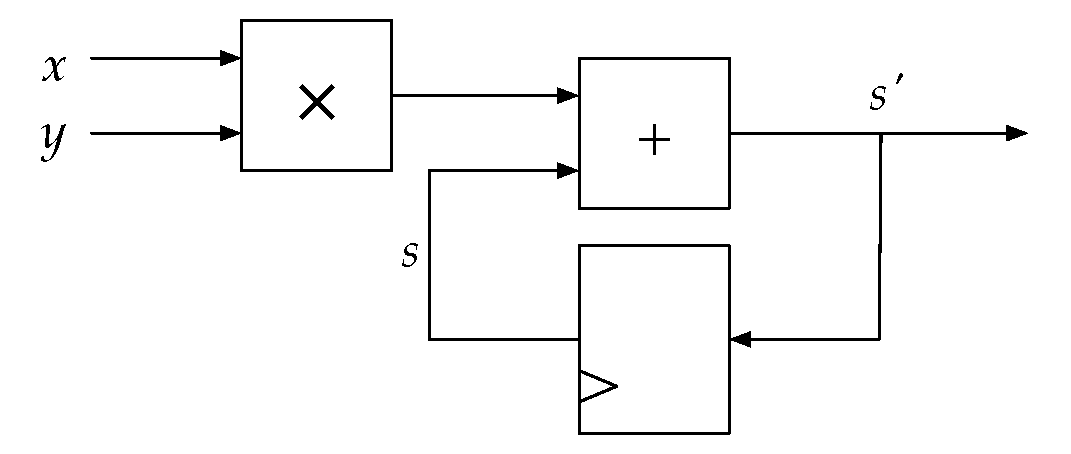
\includegraphics[width=0.6\textwidth]{images/mulaccstate}
\end{center}
\caption{Circuit of multiply-accumulate.} \label{fig:mulaccstate}
\end{figure}

Even though we have defined sequences as syntactic sugar, we are not able to use the same sequences to define feedback.
If we define a single resulting value from the feedback operation to exist at time \ensuremath{\Varid{t}}, then it depends both on the input(s) from time \ensuremath{\Varid{t}} \textit{plus} all other inputs which have had an effect on the content of the feedback register.
An obvious type for a function which represents feedback would be
\begin{changemargin}{1cm}{0cm}
\begin{expansionno}{text only}
\ensuremath{\Varid{feedback}\mathbin{::}\Conid{Int}\langle\mathrm{0}\mathinner{\ldotp\ldotp}\Varid{t}\rangle\to \Conid{Int}\langle\Varid{t}\rangle}
\end{expansionno}
\end{changemargin}
, that is, the resulting value at \ensuremath{\Varid{t}}, would depend on all values from \ensuremath{\mathrm{0}} to \ensuremath{\Varid{t}}.

The problem however, is how to define the transition from a type as \ensuremath{\Conid{Int}\langle\mathrm{0}\mathinner{\ldotp\ldotp}\Varid{t}\rangle} to \ensuremath{\Conid{Int}\langle\Varid{t}\rangle}.
Even if a way exists to describe such a transition, would it be able to accurately describe different forms of feedback?
Additional research is needed to classify different forms of feedback, and finding properties of those different classes which can be expressed by a type system.

\subsection{Multiple Clock Domains}
In this thesis, we used a single clock for entire circuits.
However, for many areas in \gls{dsp}, multiple clock domains are used.
We focus on clock domains which have different speeds, but are synchronised (e.g. the clocks do not drift).

Extending the current type-system with multiple clocks is difficult, as polytemporal types only allows a single time variable in its binder.
Either multiple time variables need to be used in order to reason about different clocks, or the relation between different clocks can be mapped to time variables in a different set of constraints.
The latter would surely make the type system very complex, making it hard to reason about the system and its soundness.
The former is also difficult, as currently the single time variable used in a polytemporal type is necessary for expressing our typing rules (page \pageref{def:typerules}).

\subsection{User defined Constraints} \label{sec:usrcon}
The constraints of our type system are currently used to reason about the compositions of time-dependent behaviour.
However, time constraints could also possibly be used to verify whether restrictions imposed on the circuit from the environment are adhered to.
For instance, two functions could be defined, both with time variables in a different scope, together with a global constraint that the time variables used by those two functions are always equal.
This would then create an additional constraint which has to be adhered to no matter how these functions are used.

\subsection{Inferred Register Placement}
Currently we do not provide an algorithm which, given a set of terms and types belonging to those terms, can determine where memory elements ought to be placed.
In this thesis we only discussed placement of memory elements very briefly, only to indicate that it should \textit{in principle} be possible.
Since the type system shows possibilities with regards to retiming, an approach which determines whether retiming is intended by the designer would be more than welcome.

\subsection{Multiple Time Variables}
We only use a single time variable to define a polytemporal type.
A single time variable is needed in order to be able to reason about the effects of time expressions under abstraction and application.
However, having more than one time variable would open up many possibilities to describe more general temporal functions.
Unfortunately, having multiple time variables makes it hard to reason about functions and their temporal constraints.
As such, this option should preferably be researched together with a different approach to expressing time as part of the type system.



\clearpage 
%% ----------------------------------------------------------------

\addtocontents{toc}{\vspace{2em}} % Add a gap in the Contents, for aesthetics

\appendix % Cue to tell LaTeX that the following 'chapters' are Appendices

\lhead[\slshape \thepage]{Appendix \thechapter. \slshape \leftmark}
%\rhead[Appendix \thechapter. \slshape \leftmark]{\slshape \thepage}
%% ODER: format ==         = "\mathrel{==}"
%% ODER: format /=         = "\neq "
%
%
\makeatletter
\@ifundefined{lhs2tex.lhs2tex.sty.read}%
  {\@namedef{lhs2tex.lhs2tex.sty.read}{}%
   \newcommand\SkipToFmtEnd{}%
   \newcommand\EndFmtInput{}%
   \long\def\SkipToFmtEnd#1\EndFmtInput{}%
  }\SkipToFmtEnd

\newcommand\ReadOnlyOnce[1]{\@ifundefined{#1}{\@namedef{#1}{}}\SkipToFmtEnd}
\DeclareFontFamily{OT1}{cmtex}{}
\DeclareFontShape{OT1}{cmtex}{m}{n}
  {<5><6><7><8>cmtex8
   <9>cmtex9
   <10><10.95><12><14.4><17.28><20.74><24.88>cmtex10}{}
\DeclareFontShape{OT1}{cmtex}{m}{it}
  {<-> ssub * cmtt/m/it}{}
\newcommand{\texfamily}{\fontfamily{cmtex}\selectfont}
\DeclareFontShape{OT1}{cmtt}{bx}{n}
  {<5><6><7><8>cmtt8
   <9>cmbtt9
   <10><10.95><12><14.4><17.28><20.74><24.88>cmbtt10}{}
\DeclareFontShape{OT1}{cmtex}{bx}{n}
  {<-> ssub * cmtt/bx/n}{}
\newcommand{\tex}[1]{\text{\texfamily#1}}	% NEU

\newcommand{\Sp}{\hskip.33334em\relax}


\newcommand{\Conid}[1]{\mathit{#1}}
\newcommand{\Varid}[1]{\mathit{#1}}
\newcommand{\anonymous}{\kern0.06em \vbox{\hrule\@width.5em}}
\newcommand{\plus}{\mathbin{+\!\!\!+}}
\newcommand{\bind}{\mathbin{>\!\!\!>\mkern-6.7mu=}}
\newcommand{\rbind}{\mathbin{=\mkern-6.7mu<\!\!\!<}}% suggested by Neil Mitchell
\newcommand{\sequ}{\mathbin{>\!\!\!>}}
\renewcommand{\leq}{\leqslant}
\renewcommand{\geq}{\geqslant}

%mathindent has to be defined
\@ifundefined{mathindent}%
  {\newdimen\mathindent\mathindent\leftmargini}%
  {}%

\def\resethooks{%
  \global\let\SaveRestoreHook\empty
  \global\let\ColumnHook\empty}
\newcommand*{\savecolumns}[1][default]%
  {\g@addto@macro\SaveRestoreHook{\savecolumns[#1]}}
\newcommand*{\restorecolumns}[1][default]%
  {\g@addto@macro\SaveRestoreHook{\restorecolumns[#1]}}
\newcommand*{\aligncolumn}[2]%
  {\g@addto@macro\ColumnHook{\column{#1}{#2}}}

\resethooks

\newcommand{\onelinecommentchars}{\quad-{}- }
\newcommand{\commentbeginchars}{\enskip\{-}
\newcommand{\commentendchars}{-\}\enskip}

\newcommand{\visiblecomments}{%
  \let\onelinecomment=\onelinecommentchars
  \let\commentbegin=\commentbeginchars
  \let\commentend=\commentendchars}

\newcommand{\invisiblecomments}{%
  \let\onelinecomment=\empty
  \let\commentbegin=\empty
  \let\commentend=\empty}

\visiblecomments

\newlength{\blanklineskip}
\setlength{\blanklineskip}{0.66084ex}

\newcommand{\hsindent}[1]{\quad}% default is fixed indentation
\let\hspre\empty
\let\hspost\empty
\newcommand{\NB}{\textbf{NB}}
\newcommand{\Todo}[1]{$\langle$\textbf{To do:}~#1$\rangle$}

\EndFmtInput
\makeatother
%
%
%
%
%
%
% This package provides two environments suitable to take the place
% of hscode, called "plainhscode" and "arrayhscode". 
%
% The plain environment surrounds each code block by vertical space,
% and it uses \abovedisplayskip and \belowdisplayskip to get spacing
% similar to formulas. Note that if these dimensions are changed,
% the spacing around displayed math formulas changes as well.
% All code is indented using \leftskip.
%
% Changed 19.08.2004 to reflect changes in colorcode. Should work with
% CodeGroup.sty.
%
\ReadOnlyOnce{polycode.fmt}%
\makeatletter

\newcommand{\hsnewpar}[1]%
  {{\parskip=0pt\parindent=0pt\par\vskip #1\noindent}}

% can be used, for instance, to redefine the code size, by setting the
% command to \small or something alike
\newcommand{\hscodestyle}{}

% The command \sethscode can be used to switch the code formatting
% behaviour by mapping the hscode environment in the subst directive
% to a new LaTeX environment.

\newcommand{\sethscode}[1]%
  {\expandafter\let\expandafter\hscode\csname #1\endcsname
   \expandafter\let\expandafter\endhscode\csname end#1\endcsname}

% "compatibility" mode restores the non-polycode.fmt layout.

\newenvironment{compathscode}%
  {\par\noindent
   \advance\leftskip\mathindent
   \hscodestyle
   \let\\=\@normalcr
   \let\hspre\(\let\hspost\)%
   \pboxed}%
  {\endpboxed\)%
   \par\noindent
   \ignorespacesafterend}

\newcommand{\compaths}{\sethscode{compathscode}}

% "plain" mode is the proposed default.
% It should now work with \centering.
% This required some changes. The old version
% is still available for reference as oldplainhscode.

\newenvironment{plainhscode}%
  {\hsnewpar\abovedisplayskip
   \advance\leftskip\mathindent
   \hscodestyle
   \let\hspre\(\let\hspost\)%
   \pboxed}%
  {\endpboxed%
   \hsnewpar\belowdisplayskip
   \ignorespacesafterend}

\newenvironment{oldplainhscode}%
  {\hsnewpar\abovedisplayskip
   \advance\leftskip\mathindent
   \hscodestyle
   \let\\=\@normalcr
   \(\pboxed}%
  {\endpboxed\)%
   \hsnewpar\belowdisplayskip
   \ignorespacesafterend}

% Here, we make plainhscode the default environment.

\newcommand{\plainhs}{\sethscode{plainhscode}}
\newcommand{\oldplainhs}{\sethscode{oldplainhscode}}
\plainhs

% The arrayhscode is like plain, but makes use of polytable's
% parray environment which disallows page breaks in code blocks.

\newenvironment{arrayhscode}%
  {\hsnewpar\abovedisplayskip
   \advance\leftskip\mathindent
   \hscodestyle
   \let\\=\@normalcr
   \(\parray}%
  {\endparray\)%
   \hsnewpar\belowdisplayskip
   \ignorespacesafterend}

\newcommand{\arrayhs}{\sethscode{arrayhscode}}

% The mathhscode environment also makes use of polytable's parray 
% environment. It is supposed to be used only inside math mode 
% (I used it to typeset the type rules in my thesis).

\newenvironment{mathhscode}%
  {\parray}{\endparray}

\newcommand{\mathhs}{\sethscode{mathhscode}}

% texths is similar to mathhs, but works in text mode.

\newenvironment{texthscode}%
  {\(\parray}{\endparray\)}

\newcommand{\texths}{\sethscode{texthscode}}

% The framed environment places code in a framed box.

\def\codeframewidth{\arrayrulewidth}

\newenvironment{framedhscode}%
  {\parskip=\abovedisplayskip\par\noindent
   \hscodestyle
   \arrayrulewidth=\codeframewidth
   \tabular{@{}|p{\linewidth-2\arraycolsep-2\arrayrulewidth-2pt}|@{}}%
   \hline\framedhslinecorrect\\{-1.5ex}%
   \let\endoflinesave=\\
   \let\\=\@normalcr
   \(\pboxed}%
  {\endpboxed\)%
   \framedhslinecorrect\endoflinesave{.5ex}\hline
   \endtabular
   \parskip=\belowdisplayskip\par\noindent
   \ignorespacesafterend}

\newcommand{\framedhslinecorrect}[2]%
  {#1[#2]}

\newcommand{\framedhs}{\sethscode{framedhscode}}

% The inlinehscode environment is an experimental environment
% that can be used to typeset displayed code inline.

\newenvironment{inlinehscode}%
  {\(\def\column##1##2{}%
   \let\>\undefined\let\<\undefined\let\\\undefined
   \newcommand\>[1][]{}\newcommand\<[1][]{}\newcommand\\[1][]{}%
   \def\fromto##1##2##3{##3}%
   \def\nextline{}}{\) }%

\newcommand{\inlinehs}{\sethscode{inlinehscode}}

% The joincode environment is a separate environment that
% can be used to surround and thereby connect multiple code
% blocks.

\newenvironment{joincode}%
  {\let\orighscode=\hscode
   \let\origendhscode=\endhscode
   \def\endhscode{\def\hscode{\endgroup\def\@currenvir{hscode}\\}\begingroup}
   %\let\SaveRestoreHook=\empty
   %\let\ColumnHook=\empty
   %\let\resethooks=\empty
   \orighscode\def\hscode{\endgroup\def\@currenvir{hscode}}}%
  {\origendhscode
   \global\let\hscode=\orighscode
   \global\let\endhscode=\origendhscode}%

\makeatother
\EndFmtInput
%

\chapter{Language Comparison} \label{ch:lang}
This chapter was written as part of a literature study to become familiar with the domain of functional hardware description languages as well as synchronous languages.
Although there are many functional hardware description languages, we only discuss \gls{forsyde}\cite{sander2004system}.
Just as there are many functional hardware description languages there are also many synchronous languages.
Having no previous experience with any of the synchronous languages available we discuss Lustre\cite{halbwachs1991synchronous}, as there also exists an extension named Pollux\cite{rocheteau1994pollux}, which allows translation from a Lustre specification to a hardware implementation.

However, before comparing both the \gls{clash} language to Lustre and \gls{forsyde}, an introduction to \gls{clash} itself is needed.
\section{C$\lambda$aSH}
\Gls{clash} is a language which leverages the language Haskell\cite{jones2003haskell}. 
Leveraging means the host language and its toolchain are modified to fulfil a different role.
In the case of \gls{clash} it means that the back-end of the \gls{ghc} compiler is replaced to allow \gls{vhdl} generation.
This does mean that updates to the \gls{ghc} compiler can not automatically be transferred to \gls{clash}.

Leveraging has some upsides however, as the entire chain of parser, lexer, type-checker, et cetera does not have to be written from scratch, but may be inherited from the host language.
Since the guest language is bound to the host language it creates a dependency on the host language, which makes it much harder to deviate from the semantics and syntax of the host language.
When deviation from the host language is required, it may be harder to facilitate this deviation when compared to a language which was created from scratch. 

Following this short introduction on how \gls{clash} relates to Haskell we will introduce the basic concepts of the language and which hardware designs it allows us to describe.

\subsection{Language basics} 
Since \gls{clash} uses Haskell it is also defined in terms of Haskell. 
Haskell is a strongly and statically typed language, which is a type of language which can catch errors in reasoning early.
This is especially nice for both rapid development and development of critical systems.

\begin{changemargin}{1cm}{0cm}
\begin{expansionno}{text only}%{On the $\lambda$-calculus}{exp:lambda}
%\small
\noindent \textbf{$\diamond$ Strong \& Static Typing} \\
While the definition of a strong type system versus a weak type system and a static type system versus a dynamic type system is not fully agreed upon, \citeauthor{o2009real} define\cite{o2009real} a strong type system as follows.

A strong type system is able to detect a class of errors in reasoning at compile-time by limiting forms of expressions.
When a type system is more restrictive in what form of expressions are allowed we can say it is strong \textit{in comparison} to another type system which is less restrictive.
In short, in a strong type system ``types cannot go wrong''\cite{milner1978theory}, as mentioned by \citeauthor{milner1978theory}.

If we take Haskell as an example for a strong type system, then C\cite{kernighan2009c} would be an example of a weak(er) type system. 
For instance, it is perfectly valid C to interpret data with a certain type as a completely unrelated type by using \textit{void} pointers. 
As such \textit{void} can be considered a hole in the type system.

This is also related to the ability to coerce (cast) a value. 
In Haskell this is not possible; we may only restrict a type, not convert one type to the other without any restriction like C allows.
For instance, the type \ensuremath{\Varid{a}} may be restricted to \ensuremath{\Conid{Int}}, but an \ensuremath{\Conid{Int}} may not be restricted to \ensuremath{\Conid{Char}} as this implies conversion.
For this purpose Haskell offers primitive functions which do allow certain conversions, for instance between an \ensuremath{\Conid{Integer}} value and a \ensuremath{\Conid{Integral}} value.

Unlike strong typing, static typing does not give additional safety directly, but merely indicates that all expressions have types, and that these types are known at compile-time.
This has the added advantage of catching errors before any code is executed, while being less flexible in dealing with run-time type changes. 
\end{expansionno}
\end{changemargin}

\gls{clash} is a synchronous language which describes circuits in a structural way.
Each component within a system is described in terms of subcomponents and can be described down to the gate level. 
By synchronous we mean that all stateful elements are updated simultaneously.
Moreover, the validity of values is limited to a certain timeframe.

\gls{clash} is structural as opposed to behavioural.
This means that the structure of an expression in the \gls{clash} language must in some form represent the expected structure of the generated hardware.
This is different from the behavioral approach where functionality is described in terms of its behavior.
When functionality is described in terms of behaviour we do not care what the resulting structure is, as long as the expected behaviour remains intact.
As a result a structural language is \textit{more} restricted when compared to a behavioural language.

\gls{clash} is excellent at describing structural forms of hardware, at least when we limit ourselves to considering combinational logic.
For instance, the circuit shown in figure \ref{fig:simplecircuit1} can easily be described in \gls{clash}, as code snippet \ref{code:simple1} shows.
As shown, \gls{clash}'s representation of the circuit is both concise and accurate in representing combinational logic.
Of course this is not the only representation, as \gls{clash} is flexible in how to define a circuit, shown by code snippets \ref{code:simple2} and \ref{code:simple3}.

\begin{figure}[H]
\begin{center}
\begin{circuitikz} \draw
(0,2) node[and port] (myand1) {}
(myand1.in 1) node[left] { $ inp1 $ }
(myand1.in 2) node[left] { $ inp2 $ }
(0,0) node[and port] (myand2) {}
(myand2.in 1) node[left] { $ inp3 $ }
(myand2.in 2) node[left] { $ inp4 $ }
(2,1) node[xnor port] (myxnor) {}
(myxnor.out) node[right] { $ out $ }
(myand1.out) -- (myxnor.in 1)
(myand2.out) -- (myxnor.in 2);
\end{circuitikz}
\end{center}
\caption{A simple combinational circuit} \label{fig:simplecircuit1}
\end{figure}

\begin{texexptitled}[text only,float]{\gls{clash} definition of a simple circuit (1)}{code:simple1}
%\begin{changemargin}{1cm}{0cm}
%\begin{expansionno}{text only}
\begin{hscode}\SaveRestoreHook
\column{B}{@{}>{\hspre}l<{\hspost}@{}}%
\column{5}{@{}>{\hspre}l<{\hspost}@{}}%
\column{9}{@{}>{\hspre}l<{\hspost}@{}}%
\column{E}{@{}>{\hspre}l<{\hspost}@{}}%
\>[B]{}\Varid{simpleCircuit}\mathbin{::}\Conid{Bit}\to \Conid{Bit}\to \Conid{Bit}\to \Conid{Bit}\to \Conid{Bit}{}\<[E]%
\\
\>[B]{}\Varid{simpleCircuit}\;\Varid{inp1}\;\Varid{inp2}\;\Varid{inp3}\;\Varid{inp4}\mathrel{=}\Varid{hwnot}\;(\Varid{hwxor}\;\Varid{s}\;\Varid{t}){}\<[E]%
\\
\>[B]{}\hsindent{5}{}\<[5]%
\>[5]{}\mathbf{where}{}\<[E]%
\\
\>[5]{}\hsindent{4}{}\<[9]%
\>[9]{}\Varid{s}\mathrel{=}\Varid{hwand}\;\Varid{inp1}\;\Varid{inp2}{}\<[E]%
\\
\>[5]{}\hsindent{4}{}\<[9]%
\>[9]{}\Varid{t}\mathrel{=}\Varid{hwand}\;\Varid{inp3}\;\Varid{inp4}{}\<[E]%
\ColumnHook
\end{hscode}\resethooks
%\end{expansionno}
%\end{changemargin}
\end{texexptitled}

\begin{texexptitled}[text only,float]{\gls{clash} definition of a simple circuit (2)}{code:simple2}
\begin{hscode}\SaveRestoreHook
\column{B}{@{}>{\hspre}l<{\hspost}@{}}%
\column{5}{@{}>{\hspre}l<{\hspost}@{}}%
\column{E}{@{}>{\hspre}l<{\hspost}@{}}%
\>[B]{}\Varid{simpleCircuit}\mathbin{::}(\Conid{Bit},\Conid{Bit},\Conid{Bit},\Conid{Bit})\to \Conid{Bit}{}\<[E]%
\\
\>[B]{}\Varid{simpleCircuit}\;(\Varid{inp1},\Varid{inp2},\Varid{inp3},\Varid{inp4})\mathrel{=}{}\<[E]%
\\
\>[B]{}\hsindent{5}{}\<[5]%
\>[5]{}\Varid{hwnot}\mathbin{\$}\Varid{hwxor}\;(\Varid{hwand}\;\Varid{inp1}\;\Varid{inp2})\;(\Varid{hwand}\;\Varid{inp3}\;\Varid{inp4}){}\<[E]%
\ColumnHook
\end{hscode}\resethooks
\end{texexptitled}

\begin{texexptitled}[text only,float]{\gls{clash} definition of a simple circuit (3)}{code:simple3}
\begin{hscode}\SaveRestoreHook
\column{B}{@{}>{\hspre}l<{\hspost}@{}}%
\column{5}{@{}>{\hspre}l<{\hspost}@{}}%
\column{9}{@{}>{\hspre}l<{\hspost}@{}}%
\column{E}{@{}>{\hspre}l<{\hspost}@{}}%
\>[B]{}\Varid{simpleCircuit}\mathbin{::}\Conid{Vector}\;\Conid{D4}\;\Conid{Bit}\to \Conid{Bit}{}\<[E]%
\\
\>[B]{}\Varid{simpleCircuit}\;\Varid{v}\mathrel{=}\Varid{hwnot}\mathbin{\$}\Varid{hwxor}\;\Varid{s}\;\Varid{t}{}\<[E]%
\\
\>[B]{}\hsindent{5}{}\<[5]%
\>[5]{}\mathbf{where}{}\<[E]%
\\
\>[5]{}\hsindent{4}{}\<[9]%
\>[9]{}\Varid{s}\mathrel{=}\Varid{hwand}\;(\Varid{v}\mathbin{!}\Varid{d2})\;(\Varid{v}\mathbin{!}\Varid{d3}){}\<[E]%
\\
\>[5]{}\hsindent{4}{}\<[9]%
\>[9]{}\Varid{t}\mathrel{=}\Varid{hwand}\;(\Varid{v}\mathbin{!}\Varid{d0})\;(\Varid{v}\mathbin{!}\Varid{d1}){}\<[E]%
\ColumnHook
\end{hscode}\resethooks
\end{texexptitled}

As can be seen in code snippet \ref{code:simple3}, \gls{clash} also supports vector types, which have type-level bounds on their size. 
Currently the length on the type-level is encoded using the $D_x$ type and with $d_x$ at the term level. 
Here, $x$ is an integer representing the number of elements a vector may have.
Since Haskell at the point of the development of \gls{clash} did not have type-level integers it was not possible to encode these directly into the type.
Instead \citeauthor{mcbride2002faking} shows\cite{mcbride2002faking} how to implement `fake' type-level integers using type families and multi-parameter type classes.
Unfortunately this has the added effect of not being as easy to use when compared to other aspects of the Haskell type system, since relatively trivial errors can not be reported in a concise manner.
This is one of the downsides of the leveraging approach mentioned earlier; we cannot modify the Haskell type system without creating our own branch of the \gls{ghc} compiler.
A recent update to \gls{ghc} allows integer literals on the type-level, which will be used in the upcoming version of the \gls{clash} compiler.
On the other hand moving the compiler to a language which supports dependent types could be considered. 
The Idris\cite{brady2011idris} language has the ability to represent true vector types at the cost of losing top-level type inference.
The leveraging approach can easily be adapted to languages such as Idris which, like Haskell, also uses a simplified normal form.
This is important as in general a simplified language is easier to translate than a more complex language, by sheer complexity.

While type-level vectors are possible in Haskell, it does not mean all work on type-level vectors is necessarily complete, as it is currently very hard, if not impossible, to make Haskell's pattern matching work with vector types. 
For instance, it would be very nice if we could rewrite the code from code snippet \ref{code:simple3} to something like the code shown in code snippet \ref{code:simple4}.

\begin{texexptitled}[text only,float]{\gls{clash} definition of a simple circuit (4)}{code:simple4}
\begin{hscode}\SaveRestoreHook
\column{B}{@{}>{\hspre}l<{\hspost}@{}}%
\column{5}{@{}>{\hspre}l<{\hspost}@{}}%
\column{E}{@{}>{\hspre}l<{\hspost}@{}}%
\>[B]{}\Varid{simpleCircuit}\mathbin{::}\Conid{Vector}\;\Conid{D4}\;\Conid{Bit}\to \Conid{Bit}{}\<[E]%
\\
\>[B]{}\Varid{simpleCircuit}\langle\Varid{v0}\mathbin{:}\Varid{v1}\mathbin{:}\Varid{v2}\mathbin{:}\Varid{v3}\rangle\mathrel{=}{}\<[E]%
\\
\>[B]{}\hsindent{5}{}\<[5]%
\>[5]{}\Varid{hwnot}\mathbin{\$}\Varid{hwxor}\;(\Varid{hwand}\;\Varid{v0}\;\Varid{v1})\;(\Varid{hwand}\;\Varid{v2}\;\Varid{v3}){}\<[E]%
\ColumnHook
\end{hscode}\resethooks
\end{texexptitled}

One option to handle this would be to use the $IsString$ typeclass.

\begin{changemargin}{1cm}{0cm}
\begin{expansionno}{text only}%{On the $\lambda$-calculus}{exp:lambda}
%\small
\noindent \textbf{$\diamond$ Typeclasses in Haskell} \\
Like many other languages the language Haskell allows a form of polymorphism.
Polymorphism is generally used to increase code reuse.
The language Haskell allows polymorphic specifications by making it possible to act on data without knowing the exact form of data.
This is done by introducing type variables.
When a type is variable it is often denoted \ensuremath{\Varid{a}}, or any other lower case letter representing the type.
This is a form of unrestricted polymorphism, where no information whatsoever is needed of the type.
One example where this is used is in functions acting on lists.
For instance, we can always take the first element of a list, as such functions work on the ``structure'' of the type.

In practice however it is often desirable to create a restricted form of polymorphism.
Typeclasses have the ablity to restrict polymorphism such that whatever form the type may take, it must implement the functions described by the typeclass in order to be well-typed.
 
For instance, if we consider the \ensuremath{\Conid{Show}} typeclass, then we must implement a function of the form \ensuremath{\Varid{show}\mathbin{::}\Varid{a}\to \Conid{String}}, which transforms the type \ensuremath{\Varid{a}} to \ensuremath{\Conid{String}}. 
We can then implement this typeclass for a type which does not have a String representation and use this type in every function which has a restriction on polymorphism in the form of \ensuremath{\Conid{Show}}. 
In those types of function the type signature would look like \ensuremath{\Conid{Show}\;\Varid{a}\Rightarrow \Varid{a}\to \Varid{a}}, which implies that for this function to have a valid type, \ensuremath{\Varid{a}} must be a valid instance of the typeclass \ensuremath{\Conid{Show}}.
\end{expansionno}
\end{changemargin}

The problem with using the $IsString$ approach is that it does not use compile-time checks, so one could write this kind of code:\\
\begin{changemargin}{1cm}{0cm}
\begin{expansionno}{text only}
\ensuremath{\Varid{select1}\mathbin{::}\Conid{Vector}\;\Conid{D2}\;\Conid{Bit}\to \Conid{Bit}}\\
\ensuremath{\Varid{select1}\;\text{\tt \char34 <v1,v2,v3,v4>\char34}\mathrel{=}\Varid{v1}}
\end{expansionno}
\end{changemargin}
and it would not cause any issues until the code is simulated.
Considering \gls{clash}'s safety properties given by its type-system we would not expect this to be possible, as the type of \ensuremath{\langle\Varid{v1},\Varid{v2},\Varid{v3},\Varid{v4}\rangle} would not be \ensuremath{\Conid{Vector}\;\Conid{D2}\;\Conid{Bit}}.
The problem could be easily avoided though if we were to create a preprocessor which solely transforms this string representation \ensuremath{\text{\tt \char34 <v1,v2,v3,v4>\char34}} to an actual representation which the Haskell type-system can reason about.
While this may solve the problem it will cause issues when error messages are to be displayed, as the Haskell type system has no knowledge about the extensions we have added.

\subsection{State representation}
State representation is particularly difficult with \gls{clash}, as compositition using stateful components is not similar to regular function application.
In ``Higher-Order Abstraction in Hardware Descriptions with ClaSH''\cite{gerards2011higher} an approach to represent state and components is introduced, by using the arrow construction used in Haskell.
A detailed introduction to arrows is out of the scope of this study, though ``Generalising monads to arrows''\cite{hughes2000generalising} may be referenced when an introduction is required.
The arrow notation is more difficult to understand, making it less suitable for hardware designers without a functional programming background.
\citeauthor{gerards2011higher} mention\cite{gerards2011higher} that all state functions which can be defined in \gls{clash} must have the following type signature:\\

\begin{changemargin}{1cm}{0cm}
\begin{expansionno}{text only}
\ensuremath{\Varid{state}\to \Varid{input}\to (\Varid{state},\Varid{output})}
\end{expansionno}
\end{changemargin}

Using this we can create a function, defined in code snippet \ref{code:sumclash}, which simply sums up all values.

\begin{texexptitled}[text only,float]{Sum as a stateful function in \gls{clash}}{code:sumclash}
\begin{hscode}\SaveRestoreHook
\column{B}{@{}>{\hspre}l<{\hspost}@{}}%
\column{5}{@{}>{\hspre}l<{\hspost}@{}}%
\column{E}{@{}>{\hspre}l<{\hspost}@{}}%
\>[B]{}\Varid{sum}\mathbin{::}\Conid{Int}\to \Conid{Int}\to (\Conid{Int},\Conid{Int}){}\<[E]%
\\
\>[B]{}\Varid{sum}\;\Varid{s}\;\Varid{i}\mathrel{=}(\Varid{s'},\Varid{s'}){}\<[E]%
\\
\>[B]{}\hsindent{5}{}\<[5]%
\>[5]{}\mathbf{where}\;\Varid{s'}\mathrel{=}\Varid{s}\mathbin{+}\Varid{i}{}\<[E]%
\ColumnHook
\end{hscode}\resethooks
\end{texexptitled}

As shown, in this case the sum is both the output as well as the state to be remembered until the next cycle.
In other cases these might be distinctly different. 

The decoupling of state and logic via the \ensuremath{\Conid{State}} datatype is necessary due to Haskell being a pure functional language. 
Since functions are primarily considered to be pure, side-effects such as statefulness can never be part of pure functions.
But when we see functions as representations of physical hardware components this becomes troublesome, as we would normally expect the state to be \textit{encapsulated} in the definition of the component.
The \ensuremath{\Varid{sum}} function from earlier would then have the type \ensuremath{\Varid{sum}\mathbin{::}\Conid{Int}\to \Conid{Int}}, with no state visible.

Stateful functions have to be defined using a specific structure of a function.
This structure can then be mapped to a component arrow, of which the definition is listed in code snippet \ref{code:comparrow}.
\begin{texexptitled}[text only,float]{Component type declaration as used in \cite{gerards2011higher}}{code:comparrow}
\begin{hscode}\SaveRestoreHook
\column{B}{@{}>{\hspre}l<{\hspost}@{}}%
\column{5}{@{}>{\hspre}l<{\hspost}@{}}%
\column{E}{@{}>{\hspre}l<{\hspost}@{}}%
\>[B]{}\mathbf{newtype}\;\Conid{Comp}\;\Varid{i}\;\Varid{o}\mathrel{=}\Conid{C}\;\{\mskip1.5mu {}\<[E]%
\\
\>[B]{}\hsindent{5}{}\<[5]%
\>[5]{}\Varid{exec}\mathbin{::}\Varid{i}\to (\Varid{o},\Conid{Comp}\;\Varid{i}\;\Varid{o}){}\<[E]%
\\
\>[B]{}\mskip1.5mu\}{}\<[E]%
\ColumnHook
\end{hscode}\resethooks
\end{texexptitled}

The details pertaining to the exact syntax of code snippet \ref{code:comparrow} are not that important, but what can be seen is a definition of a component which contains a function which, when provided with input, produces output and a new component representation. 
The notion of a continuation has already been used in the past to support Functional Reactive Programming\cite{wan2000functional,hudak2003arrows,ElliottHudak97:Fran} where arrows are also used as a basis for implementation.
Functional Reactive Programming is based on streaming and continually varying values, where functions represent behaviours which act on these continually varying values.

%\begin{changemargin}{1cm}{0cm}
%\begin{expansionno}{text only}
%\noindent \textbf{$\diamond$ Functional Reactive Programming} \\
%Functional Reactive Programming use datatypes which represent a value which changes over time by representing the history of values and making it first class in the sense that it is available for the programmer to reason about them.
%Values in FRP evolve over time and may be combined with other values. 
%Functions represent \textit{behaviors} and may be composed either sequentially or in parallel.
%A more fleshed out explanation of functional reactive programming can be found in \cite{ElliottHudak97:Fran}.
%
%One approach has been explored by \citeauthor{elliott2009push} to use discrete time and push based semantics, as opposed to the pull based semantics of most FRP implementations.
%Most FRP implementation work bottom-up, starting with the values which are needed and then `fetching' the values needed as inputs.
%According to \citeauthor{elliott2009push} this is less intuitive and makes it harder to create an efficient executable model.
%\end{expansionno}
%\end{changemargin}

Components in \gls{clash} can be created through a process called lifting using specialized function primitives.
Lifting refers to the change of perspective, where the arrow perspective is considered a higher level, component-based perspective.
Lifting then lifts a function from a low-level perspective where the state is an explicit function argument, to a high-level, component based perspective.

When lifted to the component level components can be used to compose bigger components through arrow syntax.
This lifting operation is also responsible for assigning initial state to the component.
\citeauthor{gerards2011higher} define a multiply-accumulate component as shown in code snippet \ref{code:comparrow2}, which clearly shows the decoupling between initial state and the function definition. 

\begin{texexptitled}[text only,float]{Stateful multiply-accumulate in \gls{clash}}{code:comparrow2}
\begin{hscode}\SaveRestoreHook
\column{B}{@{}>{\hspre}l<{\hspost}@{}}%
\column{5}{@{}>{\hspre}l<{\hspost}@{}}%
\column{E}{@{}>{\hspre}l<{\hspost}@{}}%
\>[B]{}\Varid{mac}\;\Varid{acc}\;(\Varid{x},\Varid{y})\mathrel{=}(\Varid{acc'},\Varid{acc'}){}\<[E]%
\\
\>[B]{}\hsindent{5}{}\<[5]%
\>[5]{}\mathbf{where}\;\Varid{acc'}\mathrel{=}\Varid{acc}\mathbin{+}\Varid{x}\mathbin{*}\Varid{y}{}\<[E]%
\ColumnHook
\end{hscode}\resethooks
\begin{hscode}\SaveRestoreHook
\column{B}{@{}>{\hspre}l<{\hspost}@{}}%
\column{E}{@{}>{\hspre}l<{\hspost}@{}}%
\>[B]{}\Varid{macA}\mathrel{=}\Varid{mac}\mathbin{`\Varid{lift}`}\mathrm{0}{}\<[E]%
\ColumnHook
\end{hscode}\resethooks
\end{texexptitled}

Ideally we would like to define this component in one function, with perhaps adding the initial state as an optional parameter.
Given these components one can use the \gls{arrow} syntax to easily control which component is connected to which component.
The syntax to use arrows was created\cite{paterson2001new} by \citeauthor{paterson2001new} after the actual arrow implementation itself. 
Without going into details here, suppose we want to define a component which combines two \ensuremath{\Varid{mac}} components in a bigger , arrow-based component.
This component, listed in code snippet \ref{code:compstmulacc}, sums the results of both \ensuremath{\Varid{mac}} components.

\begin{texexptitled}[text only,float]{Composing stateful multiply-accumulate components}{code:compstmulacc}
\begin{hscode}\SaveRestoreHook
\column{B}{@{}>{\hspre}l<{\hspost}@{}}%
\column{5}{@{}>{\hspre}l<{\hspost}@{}}%
\column{E}{@{}>{\hspre}l<{\hspost}@{}}%
\>[B]{}\Varid{twoMacAcc}\mathrel{=}\textbf{proc}\;(\Varid{w},\Varid{x},\Varid{y},\Varid{z})\to \mathbf{do}{}\<[E]%
\\
\>[B]{}\hsindent{5}{}\<[5]%
\>[5]{}\Varid{r1}\leftarrow\Varid{mac}\mathbin{`\Varid{lift}`}\mathrm{0}\prec(\Varid{w},\Varid{x}){}\<[E]%
\\
\>[B]{}\hsindent{5}{}\<[5]%
\>[5]{}\Varid{r2}\leftarrow\Varid{mac}\mathbin{`\Varid{lift}`}\mathrm{0}\prec(\Varid{y},\Varid{z}){}\<[E]%
\\
\>[B]{}\hsindent{5}{}\<[5]%
\>[5]{}\Varid{returnA}\prec\Varid{r1}\mathbin{+}\Varid{r2}{}\<[E]%
\ColumnHook
\end{hscode}\resethooks
\end{texexptitled}

There, the arguments of the component are listed as a quadruple, with its inputs listed after the \ensuremath{\textbf{proc}} keyword.
There is a lot more to be said about arrows and its syntax, but that is outside of the scope of this study.
``A new notation for arrows''\cite{paterson2001new} can be used if more information is required.

\subsection{High-level Description}
The descriptions we have seen so far were either pure functions like in code snippet \ref{code:simple1}, or component based through arrows.
Aside from these it is also possible to describe structures from a high-level perspective by merely indicating what shape the structure must take.
For instance, instead of describing a sum of a vector of integers through applying a function on each element manually , one can use higher-level functions such as \ensuremath{\Varid{foldr}}, \ensuremath{\Varid{map}} and \ensuremath{\Varid{zipWith}} which allow for more concise code. 
Additionally the same code is also faster to develop.
These functions are only available as primitives in \gls{clash} through \ensuremath{\Varid{vfoldr}},\ensuremath{\Varid{vmap}} and \ensuremath{\Varid{vzvipWith}}.
As such it is currently impossible to create custom high-level descriptions directly.

One example on how these high-level descriptions may be used is to sum values of a vector, as shown by code snippet \ref{code:sumv}.

\begin{texexptitled}[text only,float]{Sum defined over a vector of integers}{code:sumv}
\begin{hscode}\SaveRestoreHook
\column{B}{@{}>{\hspre}l<{\hspost}@{}}%
\column{E}{@{}>{\hspre}l<{\hspost}@{}}%
\>[B]{}\Varid{sumV}\mathbin{::}\Conid{Vector}\;\Conid{D4}\;\Conid{Int}\to \Conid{Int}{}\<[E]%
\\
\>[B]{}\Varid{sumV}\mathrel{=}\Varid{vfoldr}\;(\mathbin{+})\;\mathrm{0}{}\<[E]%
\ColumnHook
\end{hscode}\resethooks
\end{texexptitled}

\gls{clash} provides the following high-level descriptions:
\begin{itemize}
 \item \ensuremath{\Varid{map}}, which is used to map a function on a vector of values.
 \item \ensuremath{\Varid{vfoldr}}, which is used to fold a vector of values into a single value. Other uses are also possible depending on the function passed to the fold, e.g. a function which constructs a new vector.
 \item \ensuremath{\Varid{zipWith}}, which takes a vector of tuples and uses a function to combine both elements of the tuple into a single value. 
\end{itemize}

If a more complete description of the semantics of these functions in Haskell is required ``Real World Haskell''\cite{o2009real} or ``Learn you a Haskell''\cite{lipovaca2011learn} may be referred to.
For a more detailed look at the semantics of these functions in \gls{clash}, ``C$\lambda$aSH: From Haskell to Hardware''\cite{clashchris} may be referred to.

As mentioned before, these descriptions have a structural interpretation.
For instance, \ensuremath{\Varid{map}} represents the structure of the circuit of figure \ref{fig:map}.
Both \ensuremath{\Varid{fold}} and \ensuremath{\Varid{zipWith}} also have structural interpretations, as shown by figures \ref{fig:fold} and \ref{fig:zipWith}.
\begin{figure}
\centering
\footnotesize
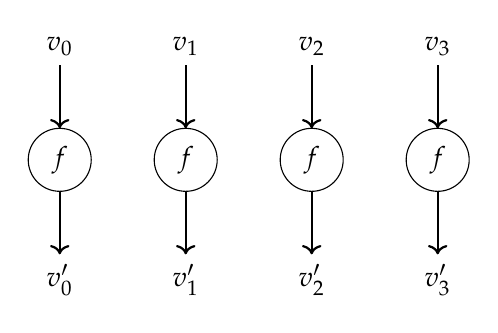
\begin{tikzpicture}[scale=0.8]
\foreach \c in {0,1,2,3} {
    \draw[->,thick] (2*\c+0.5,2) -- (2*\c+0.5,1);
    \draw[->,thick] (2*\c+0.5,0) -- (2*\c+0.5,-1);
    \draw (2*\c+0.5,0.5) circle (0.5);
    \draw (2*\c+0.5,0.5) node { $f$ };
    \draw (2*\c+0.5,2) node[above] { $v_\c$ };
    \draw (2*\c+0.5,-1) node[below] { $v'_\c$ };
}
\end{tikzpicture}
\caption{Structural interpretation of \ensuremath{\Varid{map}}} \label{fig:map}
\end{figure}

\begin{figure}[H]
\centering
\footnotesize
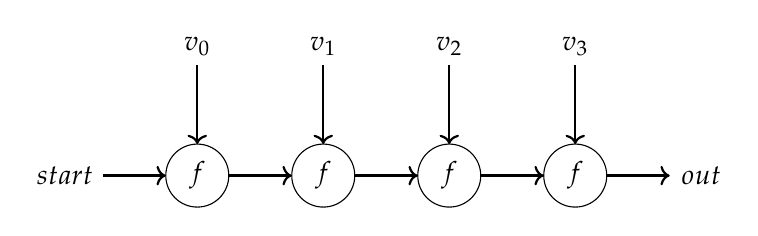
\begin{tikzpicture}[scale=0.8]
\draw (-0.25,-1.5) node[left] { $start$ };
\draw[->,thick] (-0.25,-1.5) -- (0.75,-1.5);
\foreach \c in {0,1,2,3} {
    \draw (2*\c+1.25,0.25) node[above] { $v_\c$ };
    \draw[->,thick] (2*\c+1.25,0.25) -- (2*\c+1.25,-1);
    \draw (2*\c+1.25,-1.5) node { $f$ };
    \draw (2*\c+1.25,-1.5) circle (0.5);
    \draw[->,thick] (2*\c+1.75,-1.5) -- (2*\c+2.75,-1.5);
}
\draw (9.25,-1.5) node { $out$ };
\end{tikzpicture}
\caption{Structural interpretation of \ensuremath{\Varid{vfoldr}}} \label{fig:fold}
\end{figure}

\begin{figure}[H]
\centering
\footnotesize
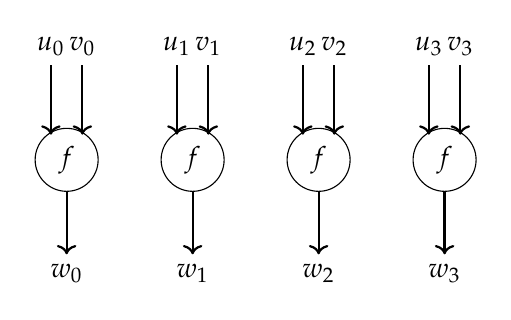
\begin{tikzpicture}[scale=0.8]
\foreach \c in {0,1,2,3} {
    \draw[->,thick] (2*\c+0.25,2) -- (2*\c+0.25,0.9);
    \draw[->,thick] (2*\c+0.75,2) -- (2*\c+0.75,0.9);
    \draw[->,thick] (2*\c+0.5,0) -- (2*\c+0.5,-1);
    \draw (2*\c+0.5,0.5) circle (0.5);
    \draw (2*\c+0.5,0.5) node { $f$ };
    \draw (2*\c+0.25,2) node[above] { $u_\c$ };
    \draw (2*\c+0.75,2) node[above] { $v_\c$ };
    \draw (2*\c+0.5,-1) node[below] { $w_\c$ };
}
\end{tikzpicture}
\caption{Structural interpretation of \ensuremath{\Varid{zipWith}}} \label{fig:zipWith}
\end{figure}

With most important features of \gls{clash} explained we can now introduce the Lustre language, after which we will compare \gls{clash} to it.

\section{Lustre}
The Lustre\cite{halbwachs1991synchronous} language is not used solely as a hardware description language.
It is used for modelling and code generation for safety critical systems.
Even though an extension in the form of Pollux\cite{rocheteau1994pollux} exists to generate hardware from these descriptions, we focus on the Lustre language itself, as more material is available to base a comparison to \gls{clash} on.
Moreover, we do not focus on the process of hardware generation, but merely on the semantical value of descriptions themselves.
Lustre was chosen as it has a number of interesting features which make it a natural match for hardware description languages, such as being synchronous and data-flow oriented.
It also allows decompositional design through nodes.

As explored in the previous section, the synchronous approach works well to create an abstract notion of time and can be used in combination with functional languages. 
Data-flow\cite{ackerman1982data} within Lustre is considered a high level programming language which enables modelling of systems using flows of data which are transformed by nodes in the flow network.
According to \citeauthor{halbwachs1991synchronous} the combination of a synchronous model and data flow languages was not investigated before, but the Lustre language combined the two by ``proposing primitives and structures which restrict data flow systems to only those which can be implemented as bounded memory automata-like programs''\cite{halbwachs1991synchronous}.

\subsection{Data representation}
Within Lustre, data is represented in the form of a \textit{flow}, which is a pair made of
\begin{itemize}
 \item A possibly infinite sequence of values of a given type;
 \item A clock, which represents the instances of time when values exist (c.q. are valid)
\end{itemize}

Since Lustre is a synchronous language, values of the clock do not correspond to any real moments in time but to abstract moments in time. 
Lustre tries to model cyclic behaviour and allows operations to directly act on flows.
From the entire program description and operations on flows the basic clock can be derived, from which all other clocks in the system can be derived. 
The basic clock is simply the smallest possible distinction between two moments in time. 
Temporal operators may be used to create slower clocks, which will be explained shortly.

When defining operations on data, Lustre always acts on the entire flow of data, e.g given a flow \ensuremath{\Conid{X}} and \ensuremath{\Conid{Y}}, the following equation:\\

\begin{changemargin}{1cm}{0cm}
\begin{expansionno}{text only}
\ensuremath{\Conid{Z}\mathrel{=}\Conid{X}\mathbin{+}\Conid{Y}}
\end{expansionno}
\end{changemargin}

is equal to\\
\begin{changemargin}{1cm}{0cm}
\begin{expansionno}{text only}
$\forall n \in \mathbb{N}_0. z_n = x_n + y_n$
\end{expansionno}
\end{changemargin}
, with $n$ being instances of time where both $x$ and $y$ exist. 

\subsection{Temporal operators}
Besides having basic arithmetic operations on flows such as addition and multiplication, Lustre also has a number of temporal operations which specifically modify flows without operating directly on the data of a flow:
\begin{itemize}
\item
    The temporal operator \ensuremath{\textbf{pre}}, shown below, allows us to define basic recursion. \\
    %\begin{texexptitled}[text only,float]{The $pre$ operation in Lustre}{code:lustrepre}

    \begin{changemargin}{1cm}{0cm}
    \begin{expansionno}{text only}
    \ensuremath{\Varid{y}\mathrel{=}\textbf{pre}\;(\Varid{x})}
    \end{expansionno} 
    \end{changemargin}% \\
    %\end{texexptitled}

    This would define a new flow, named $y$, which is simply the right shifted version of $x$. 
    This also means $y_0$, the 0\textsuperscript{th} value of the flow $y$, would have no valid value. 
    Invalid values or values which have no real value are called $nil$ within Lustre.
    The resulting flow would be \\

    \begin{changemargin}{1cm}{0cm}
    \begin{expansionno}{text only}
    $y = (nil,x_0,x_0,x_1,\ldots,x_n)$.
    \end{expansionno}
    \end{changemargin}% \\

\item
    To avoid $nil$ values regular values can be injected into the start of a flow through using the \ensuremath{\to } operator, demonstrated below.\\
    %\begin{texexptitled}[text only,float]{The $\to$ operation in Lustre}{code:lustreto}

    \begin{changemargin}{1cm}{0cm}
    \begin{expansionno}{text only}
    \ensuremath{\Varid{y}\mathrel{=}\mathrm{0}\to (\Varid{x}\mathbin{+}\textbf{pre}\;(\Varid{y}))}
    \end{expansionno}
    \end{changemargin}% \\

    This defines a flow named $y$, with $y_0$ having value $0$ and with every subsequent value being the sum of $x$ until that moment.
    The resulting flow would be \\

    \begin{changemargin}{1cm}{0cm}
    \begin{expansionno}{text only} 
    $y = (0,x_0,x_0+x_1,\ldots,\sum_{0}^{n} x_n)$.
    \end{expansionno}
    \end{changemargin}% \\

\item 
    Lustre also supports multiple clockrates through different operators, such as the \ensuremath{\textbf{when}} operator.
    The \ensuremath{\textbf{when}} operator maps a flow of booleans to a flow of values, sampling only the values on moments when the boolean flow is $true$. 
    The code below shows the mapping of the flow \ensuremath{\Varid{x}} to a clock which is twice as slow as the previous clock.\\

    \begin{changemargin}{1cm}{0cm}
    \begin{expansionno}{text only} 
    \ensuremath{\Varid{b}\mathrel{=}\Varid{true}\to (\neg \;\textbf{pre}\;(\Varid{b}))}\\
    \ensuremath{\Varid{y}\mathrel{=}\Varid{x}\;\textbf{when}\;\Varid{b}}
    \end{expansionno}
    \end{changemargin}% \\

    This defines a flow $b$ with values $(b_0,b_1,\ldots,b_n) = (true,false,true,...)$ and transforms $(x_0,x_1,\ldots,x_n)$ to $(x_0,x_2,\ldots,x_n)$ with a clock which is twice as slow as the basic clock.
\item 
    Upsampling is also possible with the exception of upsampling the basic clock. The \ensuremath{\textbf{current}} operator interpolates a flow of values to a flow of boolean values with a clock faster than its own.
    For instance, taking the flow $x = (x_0,x_2,\ldots,x_n)$ like above, applying it to the flow $(true,true,\ldots,true)$ gives a flow with values: $(x_0,x_0,x_2,x_2,\ldots,x_n,x_n)$.
\end{itemize}

\subsection{Program structure}
Of course, only being able to define expressions using the statements introduced in the previous subsection is not very useful for larger projects. 
To decompose functionality, Lustre introduces the concept of ``nodes''.
Within Lustre a flow network is a composition of nodes, in which nodes may be reused.
Code snippet \ref{code:lustrenode} shows the basic definition of a node.

\begin{texexptitled}[text only,float]{Node definition in Lustre}{code:lustrenode}
\begin{hscode}\SaveRestoreHook
\column{B}{@{}>{\hspre}l<{\hspost}@{}}%
\column{5}{@{}>{\hspre}l<{\hspost}@{}}%
\column{E}{@{}>{\hspre}l<{\hspost}@{}}%
\>[B]{}\textbf{node}\;\Conid{COUNTER}\;(\Varid{x},\Varid{y}\mathbin{:}\Varid{int};\Varid{reset}\mathbin{:}\Varid{bool})\;\Varid{returns}\;(\Varid{s},\Varid{t}\mathbin{:}\Varid{int});{}\<[E]%
\\
\>[B]{}\mathbf{let}{}\<[E]%
\\
\>[B]{}\hsindent{5}{}\<[5]%
\>[5]{}\Varid{s}\mathrel{=}\mathrm{0}\to \mathbf{if}\;\Varid{reset}\;\mathbf{then}\;\mathrm{0}\;\mathbf{else}\;\textbf{pre}\;(\Varid{s})\mathbin{+}\Varid{x}\mathbin{+}\Varid{y};{}\<[E]%
\\
\>[B]{}\hsindent{5}{}\<[5]%
\>[5]{}\Varid{t}\mathrel{=}\mathrm{0}\to \textbf{pre}\;(\Varid{t})\mathbin{+}\Varid{x}\mathbin{+}\Varid{y};{}\<[E]%
\\
\>[B]{}\textbf{tel}{}\<[E]%
\ColumnHook
\end{hscode}\resethooks
\end{texexptitled}

In the description two outputs are defined, \ensuremath{\Varid{s}} and \ensuremath{\Varid{t}}. The \ensuremath{\Varid{t}} output is defined as a sum of the previous value of \ensuremath{\Varid{t}}, combined with the addition of \ensuremath{\Varid{x}} and \ensuremath{\Varid{y}}.
The output \ensuremath{\Varid{s}} is defined to be \ensuremath{\mathrm{0}} when the reset input is toggled, otherwise it will sum the previous value of \ensuremath{\Varid{s}} together with \ensuremath{\Varid{x}} and \ensuremath{\Varid{y}}. 
In this example \ensuremath{\Varid{s}} represents a partial summation, while \ensuremath{\Varid{t}} represents a total summation.

Reusing nodes is also straightforward, as it is much like function application. 
For instance, the node from code snippet \ref{code:lustrereuse} uses the $COUNTER$ from before to sum three consecutive sums of $x$ and $y$ and the total sum. 
In that example the reset is switched every three cycles, while \ensuremath{\Varid{x}} and \ensuremath{\Varid{y}} are summed in \ensuremath{\Varid{s}} only when the reset is \ensuremath{\Varid{false}}.

\begin{texexptitled}[text only,float]{Node reusing in Lustre}{code:lustrereuse}
\begin{hscode}\SaveRestoreHook
\column{B}{@{}>{\hspre}l<{\hspost}@{}}%
\column{5}{@{}>{\hspre}l<{\hspost}@{}}%
\column{11}{@{}>{\hspre}l<{\hspost}@{}}%
\column{E}{@{}>{\hspre}l<{\hspost}@{}}%
\>[B]{}\textbf{node}\;\Conid{SUM3}\;(\Varid{x},\Varid{y}\mathbin{:}\Varid{int})\;\Varid{returns}\;(\Varid{s},\Varid{t}\mathbin{:}\Varid{int});{}\<[E]%
\\
\>[B]{}\mathbf{let}{}\<[E]%
\\
\>[B]{}\hsindent{5}{}\<[5]%
\>[5]{}\Varid{rst}{}\<[11]%
\>[11]{}\mathrel{=}\mathrm{0}\to \mathbf{if}\;(\textbf{pre}\;(\Varid{rst})\mathrel{=}\mathrm{5})\;\mathbf{then}\;\mathrm{0}\;\mathbf{else}\;\textbf{pre}\;(\Varid{rst})\mathbin{+}\mathrm{1};{}\<[E]%
\\
\>[B]{}\hsindent{5}{}\<[5]%
\>[5]{}(\Varid{s},\Varid{t})\mathrel{=}\Conid{COUNTER}\;(\Varid{x},\Varid{y},\Varid{rst}\langle\mathrm{3});{}\<[E]%
\\
\>[B]{}\textbf{tel}{}\<[E]%
\ColumnHook
\end{hscode}\resethooks
\end{texexptitled}

\FloatBarrier
From observing code snippet \ref{code:lustrereuse} we can conclude the following:
\begin{enumerate}
\item  it would be nice to have integer references to previous points in time, so we would be able to write something as\\

\begin{changemargin}{1cm}{0cm}
\begin{expansionno}{text only}
\ensuremath{\Varid{rst}\mathrel{=}\Varid{repeat}\;\mathrm{3}\;\Varid{true}\to (\neg \;\textbf{pre}\;(\mathrm{3},\Varid{rst}))}
\end{expansionno}
\end{changemargin}% \\

, which is a lot clearer and to the point.
The \ensuremath{\Varid{repeat}} operation would then result into a flow $(true,true,true,nil,nil,\ldots,nil)$, after which \ensuremath{\neg \;\textbf{pre}\;(\mathrm{3},\Varid{rst})} defines the remaining cyclic behaviour by generating the next three values as the inverse of the last known value of the flow.
\item Compositions of nodes only show the inputs and outputs of the composition. As a result, when composing nodes, the original definitions of the nodes have to be consulted to reason about the behaviour of the composition. 
\end{enumerate}

Lustre also allows assertions for runtime verification and code generation optimization. 
For instance the assertion \\
\begin{changemargin}{1cm}{0cm}
\begin{expansionno}{text only}
\ensuremath{\textbf{assert}\;\neg \;(\Varid{x}\;\Varid{and}\;\Varid{y});}
\end{expansionno}
\end{changemargin}

will trigger a run-time assertion error if $x$ and $y$ are both true. 
Lustre will also use this to help with code generation, though details on how this is done are not listed.
While run-time assertions are nice to have, for critical applications it is not desirable to merely have error signalling without error handling.
This is especially the case in the context hardware architectures where performance is required.

\subsection{Arrays and recursion}
To allow high-level constructs arrays were introduced to Lustre at version 4. 
Basically these work like vectors in \gls{clash} and \gls{vhdl}.
The sizes of these types have to be known at compile-time, as Lustre simply expands each array depending on how many elements it has. 
This is not really a problem, unless one wants to reuse a design and parameterization is required, as Lustre does not support it.

\citeauthor{halbwachs1993tutorial} show\cite{halbwachs1993tutorial} some examples and details concerning array syntax, which we will briefly repeat here.
For instance, code snippet \ref{code:lustreripple} shows a ripple carry adder using an array of four full adders.
\begin{texexptitled}[text only,float]{Ripple carry adder in Lustre}{code:lustreripple}
\begin{hscode}\SaveRestoreHook
\column{B}{@{}>{\hspre}l<{\hspost}@{}}%
\column{5}{@{}>{\hspre}l<{\hspost}@{}}%
\column{13}{@{}>{\hspre}l<{\hspost}@{}}%
\column{25}{@{}>{\hspre}l<{\hspost}@{}}%
\column{E}{@{}>{\hspre}l<{\hspost}@{}}%
\>[B]{}\textbf{node}\;\Conid{ADD1}\;(\Varid{a},\Varid{b},c_i\mathbin{:}\Varid{bool})\;\Varid{returns}\;(\Varid{s},c_o\mathbin{:}\Varid{bool});{}\<[E]%
\\
\>[B]{}\mathbf{let}{}\<[E]%
\\
\>[B]{}\hsindent{5}{}\<[5]%
\>[5]{}\Varid{s}{}\<[13]%
\>[13]{}\mathrel{=}\Varid{a}\;\Varid{xor}\;\Varid{b}\;\Varid{xor}\;c_i;{}\<[E]%
\\
\>[B]{}\hsindent{5}{}\<[5]%
\>[5]{}c_o{}\<[13]%
\>[13]{}\mathrel{=}(\Varid{a}\;\Varid{and}\;\Varid{b})\;\Varid{or}\;(\Varid{b}\;\Varid{and}\;c_i)\;\Varid{or}\;(c_i\;\Varid{and}\;\Varid{a});{}\<[E]%
\\
\>[B]{}\textbf{tel}{}\<[E]%
\\[\blanklineskip]%
\>[B]{}\textbf{node}\;\Conid{ADD4}\;(\Conid{A},\Conid{B}\mathbin{:}\Varid{bool}^\mathrm{4})\;\Varid{returns}\;(\Conid{S}\mathbin{:}\Varid{bool}^\mathrm{4},\Varid{carry}\mathbin{:}\Varid{bool}){}\<[E]%
\\
\>[B]{}\Varid{var}\;\Conid{C}\mathbin{:}\Varid{bool}^\mathrm{4};{}\<[E]%
\\
\>[B]{}\mathbf{let}{}\<[E]%
\\
\>[B]{}\hsindent{5}{}\<[5]%
\>[5]{}(\Conid{S}\;[\mskip1.5mu \mathrm{0}\mskip1.5mu],\Conid{C}\;[\mskip1.5mu \mathrm{0}\mskip1.5mu]){}\<[25]%
\>[25]{}\mathrel{=}\Conid{ADD1}\;(\Conid{A}\;[\mskip1.5mu \mathrm{0}\mskip1.5mu],\Conid{B}\;[\mskip1.5mu \mathrm{0}\mskip1.5mu],\Varid{false}){}\<[E]%
\\
\>[B]{}\hsindent{5}{}\<[5]%
\>[5]{}(\Conid{S}\;[\mskip1.5mu \mathrm{1}\mathinner{\ldotp\ldotp}\mathrm{3}\mskip1.5mu],\Conid{C}\;[\mskip1.5mu \mathrm{1}\mathinner{\ldotp\ldotp}\mathrm{3}\mskip1.5mu]){}\<[25]%
\>[25]{}\mathrel{=}\Conid{ADD1}\;(\Conid{A}\;[\mskip1.5mu \mathrm{1}\mathinner{\ldotp\ldotp}\mathrm{3}\mskip1.5mu],\Conid{B}\;[\mskip1.5mu \mathrm{1}\mathinner{\ldotp\ldotp}\mathrm{3}\mskip1.5mu],\Conid{C}\;[\mskip1.5mu \mathrm{1}\mathinner{\ldotp\ldotp}\mathrm{3}\mskip1.5mu]);{}\<[E]%
\\
\>[B]{}\hsindent{5}{}\<[5]%
\>[5]{}\Varid{carry}{}\<[25]%
\>[25]{}\mathrel{=}\Conid{C}\;[\mskip1.5mu \mathrm{3}\mskip1.5mu];{}\<[E]%
\\
\>[B]{}\textbf{tel}{}\<[E]%
\ColumnHook
\end{hscode}\resethooks
\end{texexptitled}

The $ADD1$ node is a straightforward implementation of a full adder, which is then used in the ripple carry definition. 
The ripple carry is less straightforward, especially the second equation as it applies an array to a node which only accepts single flows, not arrays of flows.
Lustre allows this sort of behavior, as the compiler can reason about definitions such as these since it only uses compile-time size definitions. 
\citeauthor{halbwachs1993tutorial} call\cite{halbwachs1993tutorial} this polymorphism, but since this does not allow any length of arrays to be used, it is a limited kind of polymorphism. 

Lustre only supports a very specific kind of recursion which is based on being able to determine when the recursion terminates at compile-time.
This is related to totality in programming, a practice where partial functions are not allowed.
Partial functions are undefined for a subset of their domain, which is needed to support general recursion.
Recursion in Lustre is defined by a function which has a certain number of inputs and one constant which is know at compile-time. 
This constant needs to be part of the terminating condition and is needed to unroll the recursion at compile-time.
Code snippet \ref{code:lustrerec} shows the basic principle.

\begin{texexptitled}[text only,float]{Halting recursion in Lustre}{code:lustrerec}
\begin{hscode}\SaveRestoreHook
\column{B}{@{}>{\hspre}l<{\hspost}@{}}%
\column{5}{@{}>{\hspre}l<{\hspost}@{}}%
\column{7}{@{}>{\hspre}l<{\hspost}@{}}%
\column{E}{@{}>{\hspre}l<{\hspost}@{}}%
\>[B]{}\textbf{node}\;\Conid{REC}\;(\Varid{const}\;\Varid{x}\mathbin{:}\Varid{int};\Varid{y}\mathbin{:}\Varid{int})\;\Varid{returns}\;(\Varid{z}\mathbin{:}\Varid{int}){}\<[E]%
\\
\>[B]{}\mathbf{let}{}\<[E]%
\\
\>[B]{}\hsindent{5}{}\<[5]%
\>[5]{}\textbf{with}\;\Varid{x}\mathrel{=}\mathrm{0}{}\<[E]%
\\
\>[5]{}\hsindent{2}{}\<[7]%
\>[7]{}\mathbf{then}\;\Varid{y}{}\<[E]%
\\
\>[5]{}\hsindent{2}{}\<[7]%
\>[7]{}\mathbf{else}\;\Varid{y}\mathbin{+}\Conid{REC}\;(\Varid{x}\mathbin{-}\mathrm{1},\Varid{y});{}\<[E]%
\\
\>[B]{}\textbf{tel}{}\<[E]%
\ColumnHook
\end{hscode}\resethooks
\end{texexptitled}

The above code simply multiplies one input with the other by using the plus operator, e.g. rewriting multiplication as a series of addition.
It is important that \ensuremath{\Varid{x}} is a constant value here, that is, there is one value which \ensuremath{\Varid{x}} represents, and this value may not change during the process defined in this node.
Since this is a constant value it is known at compile-time and as such can be used to unroll the recursion.

We can also define a recurrence relation which captures the essence of recursion.
A sequence of the natural numbers can be defined using the $\rightarrow$ and \ensuremath{\textbf{pre}} operators:\\
\begin{changemargin}{1cm}{0cm}
\begin{expansionno}{text only}
\ensuremath{\Varid{c}\mathrel{=}\mathrm{0}\to \textbf{pre}\;(\Varid{c})\mathbin{+}\mathrm{1};}.
\end{expansionno}
\end{changemargin}

\subsection{Comparison of C$\lambda$aSH and Lustre}
With the basic concepts of both \gls{clash} as Lustre explained we can now compare the two languages.
At first glance both languages seem to have little in common, as Lustre is not really a hardware description language, even though it can be used to model hardware.
However, we can look at its syntax and paradigm and compare those.

Lustre is built around flows, making distinct moments in time explicit. 
It also allows us to refer to previous values of a flow and as such is a stream-based approach.
This can be considered a more behavioural approach when compared to \gls{clash}.
Within \gls{clash} one would have to explicitly store and move values around to achieve the same effect as Lustre, as shown in code snippet \ref{code:clash3cons}, as \gls{clash} is a structural language where we name wires or values.
\begin{texexptitled}[text only,float]{Sum of the last three consecutive values in \gls{clash}}{code:clash3cons}
\begin{hscode}\SaveRestoreHook
\column{B}{@{}>{\hspre}l<{\hspost}@{}}%
\column{5}{@{}>{\hspre}l<{\hspost}@{}}%
\column{9}{@{}>{\hspre}l<{\hspost}@{}}%
\column{E}{@{}>{\hspre}l<{\hspost}@{}}%
\>[B]{}\Varid{add3}\mathbin{::}(\Conid{Int},\Conid{Int})\to \Conid{Int}\to ((\Conid{Int},\Conid{Int}),\Conid{Int}){}\<[E]%
\\
\>[B]{}\Varid{add3}\;(\Varid{s1},\Varid{s2})\;\Varid{i}\mathrel{=}((\Varid{s1'},\Varid{s2'}),\Varid{o}){}\<[E]%
\\
\>[B]{}\hsindent{5}{}\<[5]%
\>[5]{}\mathbf{where}{}\<[E]%
\\
\>[5]{}\hsindent{4}{}\<[9]%
\>[9]{}\Varid{s1'}\mathrel{=}\Varid{i}{}\<[E]%
\\
\>[5]{}\hsindent{4}{}\<[9]%
\>[9]{}\Varid{s2'}\mathrel{=}\Varid{s1}{}\<[E]%
\\
\>[5]{}\hsindent{4}{}\<[9]%
\>[9]{}\Varid{o}\mathrel{=}\Varid{i}\mathbin{+}\Varid{s1}\mathbin{+}\Varid{s2}{}\<[E]%
\ColumnHook
\end{hscode}\resethooks
\end{texexptitled}

Of course, there are also alternatives, such as constructing a single register and using arrow notation to combine two of these into a final component. 
This does not increase the readability however, as it is hard to keep track of how values are used.
The structural approach makes it easy to reason about the resulting hardware representation, yet it is hard to discern what the structure is from this piece of code.

Lustre's syntax makes this more concise, as shown in code snippet \ref{code:lustre3cons}, though the lack of relative indexing of flows is still not very elegant.
The Lustre code is more concise and actually explains how $add3$ should behave in time relative to a certain point, where the \gls{clash} code is still about manipulating values and ``where'' they should go.

\begin{texexptitled}[text only,float]{Sum of the last three consecutive values in Lustre}{code:lustre3cons}
\begin{hscode}\SaveRestoreHook
\column{B}{@{}>{\hspre}l<{\hspost}@{}}%
\column{5}{@{}>{\hspre}l<{\hspost}@{}}%
\column{E}{@{}>{\hspre}l<{\hspost}@{}}%
\>[B]{}\textbf{node}\;\Conid{ADD3}\;(\Varid{i}\mathbin{:}\Varid{int})\;\Varid{returns}\;(\Varid{o}\mathbin{:}\Varid{int});{}\<[E]%
\\
\>[B]{}\mathbf{let}{}\<[E]%
\\
\>[B]{}\hsindent{5}{}\<[5]%
\>[5]{}\Varid{o}\mathrel{=}\textbf{pre}\;(\Varid{i})\mathbin{+}\textbf{pre}\;(\textbf{pre}\;(\Varid{i}))\mathbin{+}\Varid{i};{}\<[E]%
\\
\>[B]{}\textbf{tel}{}\<[E]%
\ColumnHook
\end{hscode}\resethooks
\end{texexptitled}

Aside from the flow aspect, Lustre also offers multiple clocks, although all of these are assumed to be synchronized. 
The same could be implemented in \gls{clash}, although support for this is currently not available. 
The \ensuremath{\textbf{when}} and \ensuremath{\textbf{current}} statements make it easy to upsample or downsample a given clock, which is not implemented concisely in \gls{clash} in its current state.

Of course, \gls{clash} is a language which is specifically designed for hardware description, while Lustre only allow hardware generation through Pollux.
Even so, Lustre gives some nice insights into state, especially how state can be considered a temporal phenomenon. 
Lustre can easily do this because, while it does not allow cyclic definitions entirely, it does allow cycles when a \ensuremath{\textbf{pre}} operator is present. 
A description such as \\
\begin{changemargin}{1cm}{0cm}
\begin{expansionno}{text only}
\ensuremath{\Varid{x}\mathrel{=}\mathrm{0}\to \textbf{pre}\;(\Varid{x})\mathbin{+}\textbf{pre}\;(\Varid{x});}
\end{expansionno}
\end{changemargin}
would not be possible in \gls{clash} without using some form of flow or a state machine which represents such a flow.
It is unfair however to view Lustre's recursive definitions as superior to \gls{clash}'s arrow-based components, as it is perfectly possible to define sequential logic in \gls{clash}. 
However, as \gls{clash} is a functional language, a more ``pure'' recursive specification would be preferable, which is exactly what Lustre offers.

Additionally, both Lustre and \gls{clash} allow bounded vectors or arrays. 
In Lustre it is very easy to create slices, also known as subvectors, from vectors, while it remains a bit cumbersome in \gls{clash}, due to the nature of the host language Haskell.

However, one major advantage \gls{clash} has over Lustre is the type system.
Since \gls{clash} allows type inference, it is possible for a designer to query the type system; the type system can aid the designer.
Type inference allows the compiler to derive types from the structure of expressions themselves.
In Lustre, when an error is encountered it is hard to find out exactly what went wrong, as the Lustre verification only points us in the right direction. 
It never concisely points out what the actual error is.
In \gls{clash} the verification \textit{is} the type system, and as such provides the programmer with a hands-on tool to interface with the compiler, leading to a reduction in time spent to find bugs or faulty logic.



\section{ForSyDe}
The \gls{forsyde}\cite{sander2004system} language, like \gls{clash}, uses the language Haskell to provide a new language te develop embedded systems.
At first the language was focussed on simply modelling systems in general and simulating the descriptions using the \gls{ghc} interpreter. 
With the addition of \gls{vhdl} generation\cite{acosta2007hardware} it became a language in which one can model and synthesize hardware descriptions.
The hardware description capabilities are the parts which this section will focus on.

\gls{forsyde} is a language which currently only supports synchronous systems, approach used by many other hardware description languages as well.
Many hardware description languages use a synchronous model of time as it is relatively simple to simulate. 
It also is an easy model from the designer's perspective.
\gls{forsyde}, unlike \gls{clash}, uses the \gls{edsl} approach to avoid the effort needed to create a compiler, type-checker, et cetera from scratch.
A \gls{dsl} is, as its name implies, a language designed specifically with one domain in mind.
A \gls{edsl} however, is a specific kind of \gls{dsl}, which uses a host language in which the guest language is \tif{embedded}.
Embedding a language has some advantages, like using existing syntax, tools of the host language, and not needing to develop an entire compiler from scratch. 
The \gls{edsl} approach does not offer many advantages over the leveraging approach used by \gls{clash}, a property which will be discussed later in more detail.
For now it is enough to know that leveraging binds a language to a specific \textit{implementation}, while the \gls{edsl} approach binds a language to a specific \textit{language}.
In practice \gls{ghc} is the defacto standard compiler for Haskell, and as such there is not much difference in dependence on either the language or the specific implementation.

\subsection{Processes}
Within ForSyDe, systems are modelled using an abstraction called processes. 
These processes can be combined through networks. 
This approach is very similar to data-flow approaches discussed before.
Perhaps unsurprisingly, \gls{forsyde} uses Haskell's list structure to represent signals.
A process can then be seen as a function which transforms one signal to another signal.
However, as functions operate on entire signals, it is harder for a compiler to discern what \textit{elements} of the signal are used.
This makes it harder to do optimalizations based on these descriptions, since functions which are referential transparent with regards to the elements of a signal offer many ways to optimize code, a quality which is often associated with Haskell.

The fact that signals are needed in \gls{forsyde} can be seen in how processes are defined.
\gls{forsyde} supplies a number of process constructors which take a function as input, an approach often used in Haskell. 
First, they define a signal in the style of lists with \ensuremath{\coloneq} as the Signal constructor
\begin{changemargin}{1cm}{0cm}
\begin{expansionno}{text only}
\ensuremath{\mathbf{data}\;\Conid{Signal}\;\Varid{a}\mathrel{=}\Varid{a}\coloneq\Conid{Signal}\;\Varid{a}}
\ensuremath{| \Conid{NullS}}
\end{expansionno}
\end{changemargin}
, which is used in the definition of the \ensuremath{\Varid{mapSY}} constructor, shown by code snippet \ref{code:formapsy}.

\begin{texexptitled}[text only,float]{The \ensuremath{\Varid{mapSY}} process constructor in \gls{forsyde}}{code:formapsy}
\begin{hscode}\SaveRestoreHook
\column{B}{@{}>{\hspre}l<{\hspost}@{}}%
\column{17}{@{}>{\hspre}l<{\hspost}@{}}%
\column{E}{@{}>{\hspre}l<{\hspost}@{}}%
\>[B]{}\Varid{mapSY}\mathbin{::}(\Varid{a}\to \Varid{b})\to \Conid{Signal}\;\Varid{a}\to \Conid{Signal}\;\Varid{b}{}\<[E]%
\\
\>[B]{}\Varid{mapSY}\;\anonymous \;\Conid{NullS}{}\<[17]%
\>[17]{}\mathrel{=}\Conid{NullS}{}\<[E]%
\\
\>[B]{}\Varid{mapSY}\;\Varid{f}\;(\Varid{x}\coloneq\Varid{xs})\mathrel{=}\Varid{f}\;\Varid{x}\coloneq(\Varid{mapSY}\;\Varid{f}\;\Varid{xs}){}\<[E]%
\ColumnHook
\end{hscode}\resethooks
\end{texexptitled}
The process resulting from \ensuremath{\Varid{mapSY}} clearly behaves the same as a regular \ensuremath{\Varid{map}} function over lists as is commonly used in Haskell.

Aside from \ensuremath{\Varid{mapSY}}, \gls{forsyde} also supplies the following process constructors:
\begin{itemize}
 \item \ensuremath{\Varid{zipWithSY}}, which is analogous to \ensuremath{\Varid{zipWith}} from Haskell; it takes two \ensuremath{\Conid{Signal}}s and uses a function to combine these \ensuremath{\Conid{Signal}}s into one.
\item \textit{delaySY$_k$}, which delays a \ensuremath{\Conid{Signal}} with $k$ discrete time steps. It can be used to create feedback, for instance to create the \ensuremath{\Varid{sourceSY}} constructor.
\item \ensuremath{\Varid{sourceSY}}, which generates an infinite series of outputs.
\item \ensuremath{\Varid{scanlSY}}, which acts much like the the \ensuremath{\Varid{scanl}} of Haskell. 
When thinking of streams it makes sense to use \ensuremath{\Varid{scanl}} to encapsulate state. 
A stream of values together with a function which acts on two individual elements of the stream can then be used to `store' intermediate results. 
Of course, since these intermediate results only depend on the previous values of the Signal and the function applied to it it is still a pure function. 
\item \ensuremath{\Varid{mooreSY}}, a constructor for a Moore machine; a process from which the output only depends on the internal state.
\item \ensuremath{\Varid{mealySY}}, a constructor for a Mealy machine; a process from which the output depends on both the internal state and the input signals.
\item \ensuremath{\Varid{unzipSY}}, which is analogous to the \ensuremath{\Varid{unzip}} function in Haskell. 
\end{itemize}

These process constructors can be composed to create new, more complex processes, as in code snippet \ref{code:formulacc}.
\begin{texexptitled}[text only,float]{Stateful multiply-accumulate in \gls{forsyde}}{code:formulacc}
\begin{hscode}\SaveRestoreHook
\column{B}{@{}>{\hspre}l<{\hspost}@{}}%
\column{5}{@{}>{\hspre}l<{\hspost}@{}}%
\column{9}{@{}>{\hspre}l<{\hspost}@{}}%
\column{E}{@{}>{\hspre}l<{\hspost}@{}}%
\>[B]{}\Varid{macSY}\mathbin{::}\Conid{Num}\;\Varid{a}\Rightarrow \Conid{Signal}\;\Varid{a}\to \Conid{Signal}\;\Varid{a}\to \Conid{Signal}\;\Varid{a}{}\<[E]%
\\
\>[B]{}\Varid{macSY}\;\Varid{x}\;\Varid{y}\mathrel{=}\Varid{scanlSY}\;(\mathbin{+})\;\mathrm{0}\;\Varid{prod}{}\<[E]%
\\
\>[B]{}\hsindent{5}{}\<[5]%
\>[5]{}\mathbf{where}{}\<[E]%
\\
\>[5]{}\hsindent{4}{}\<[9]%
\>[9]{}\Varid{prod}\mathrel{=}\Varid{zipWithSY}\;(\mathbin{*})\;\Varid{x}\;\Varid{y}{}\<[E]%
\ColumnHook
\end{hscode}\resethooks
\end{texexptitled}

This is equivalent to the following Haskell code using lists:
\begin{changemargin}{1cm}{0cm}
\begin{expansionno}{text only}
\ensuremath{\Varid{mac}\;\Varid{xs}\;\Varid{ys}\mathrel{=}\Varid{scanl}\;(\mathbin{+})\;\mathrm{0}\;(\Varid{zipWith}\;(\mathbin{*})\;\Varid{xs}\;\Varid{ys})}
\end{expansionno}
\end{changemargin}
\citeauthor{sander2004system} list\cite{sander2004system} more detailed examples, but this example should be enough to explain the principle.

\subsection{Deep and shallow embedding}
While not mentioned before, the only way to generate \gls{vhdl} from a \gls{forsyde} model is to use the so-called ``deeply embedded'' approach. 
The regular \gls{forsyde} model does not contain the information needed to generate \gls{vhdl} code.
This is due to the fact the language is embedded in the host language.
Since it is embedded in the host language, it is restricted by the host language as well.
This restriction has certain downsides, as one would normally not be able to \tif{observe sharing} within a certain program, functionality which is needed to detect cycles in a program.
Cycles are often needed in hardware descriptions to describe feedback, so observable sharing is necessary.
Fortunately Lava\cite{claessen2002embedded,bjesse1998lava} faced the same problems at an earlier stage and solved this through observable sharing\cite{claessen1999observable}.

In order to use this a non-backwards compatible change had to be made, which is referred to as the ``deeply embedded'' approach. 
This approach heavily depends on using Template Haskell, which makes the \gls{ast} of the program c.q. hardware description accessible from within the language itself.
The usage of Template Haskell introduces several problems, which will be looked at in detail in the comparison with \gls{clash}.
The gist of it is however that to use functionality many Haskell programmers take for granted, such as polymorphism and higher order functions, functions that depend on them need to have a specific type signature.
These functions must then be passed into Quasi-Quatation\cite{sheard2002template} blocks, all of which only hinder readability and do nothing to aid the designer.

\subsection{Program structure}
To provide more structure to the hardware design, the designer has the ability to define circuit definitions using hierachical structures. 
These structures have a strong relation with the structures used in \gls{vhdl}, probably both for reasons of familiarity as well as ease of translation. 
\gls{forsyde} supplies the following hierachical structures:
\begin{itemize}
\item 
A \ensuremath{\Conid{Port}} is almost identical to \gls{vhdl}'s port clause, aside from the fact that in \gls{forsyde} it is not allowed to mix input and output ports; two separate ports have to be made per system, provided they indeed have both in and output ports. 
The port structure serves as an interface between the outside world and the system. 
However, there wasn't a lot of concrete information available as to what the actual use of this structure is. 
Since it is so closely related to \gls{vhdl} it seems natural to use these interfaces to mix regular \gls{vhdl} code with generated \gls{vhdl} code. 
These ports are named \ensuremath{\Conid{InPort}} and \ensuremath{\Conid{OutPort}} and consist of a list of tuples containing the name and the type of each input or output.
\item A \ensuremath{\Conid{Circuit}} is defined as a function which transforms an \ensuremath{\Conid{InPort}} to an \ensuremath{\Conid{OutPort}}. The circuit definition then simply consists of applying functions to the specific input ports of the circuit.
\item The circuits defined can then be turned into a \ensuremath{\Conid{Block}}, which is a white-box which can not be connected directly to other system structures. A \ensuremath{\Conid{Block}} can be instantiated, or transformed into a \ensuremath{\Conid{BlockIns}} structure.
This structure is a black-box, but its inputs and outputs can be used to connect to other parts of the system. 
A \ensuremath{\Conid{Block}} and \ensuremath{\Conid{BlockIns}} are similar to entity-architecture pairs and component in \gls{vhdl}. 
\end{itemize}

\subsection{Arrays and Vectors}
Vectors in \gls{clash} are not much different from those used in \gls{forsyde} as the library introduced\cite{acosta2008forsyde} by \citeauthor{acosta2008forsyde} was used as an inspiration for \gls{clash} as mentioned in ``Clash: From Haskell to Hardware''\cite{clashchris}.
As such it is not very interesting to go into details, as any comparison will simply state they are very similar and offer the same advantages and disadvantages. 
We already discussed the advantages and disadvantages of this approach in the context of \gls{clash} in a previous section.

\subsection{Comparison of C$\lambda$aSH and ForSyDe}
\gls{clash} and \gls{forsyde} seem to have a lot in common. 
They both use Haskell, albeit in different ways.
The methods used to translate the model is different, as well as the model itself and the way this model is presented to the designer.

\gls{forsyde} is a language which makes streaming explicit and allows the designer to create processes which act on these streams.
\gls{clash} on the other hand does not deal with streams at all and is more structural in its approach, allowing the designer to define a circuit in terms of \tif{wires} or \tif{individual values}, not in \textit{streams} of values. 
\gls{clash} is able to describe a circuit structurally because it is able to transform a program description from the outside of the language it is created in.
This is not the case for \gls{forsyde}, as it can only analyze whatever the language Haskell and its \gls{ghc} implementation allow it to analyze. 

As mentioned before, \gls{clash} leverages Haskell and as such is bound tightly to a specific implementation of \gls{ghc}.
In \gls{clash} the translation is done outside the programming environment of Haskell, so it can look from the outside in and has access to Haskell's Core language to transform definitions from the Haskell source straight to \gls{vhdl}.
This is different from the \gls{forsyde} approach, which uses Template Haskell to access the \gls{ast} of the program from within the limits of the language it is embedded in.
This limits on the translation of \tif{user defined} descriptions:
\begin{itemize}
 \item When defining a function and passing it to a process constructor the number of parameters must equal the number of arguments; currying is not allowed.
 \item The signature of the function supplied to the process constructor has to be made explicit, regardless of the function.
 \item Pattern matching is limited to literals, variables and wildcards; no pattern matching on data constructors is allowed.
 \item \ensuremath{\mathbf{where}} and \ensuremath{\mathbf{let}} clauses are not allowed.
 \item Polymorphism is only supported for instances of a certain typeclass. 
 In ``Hardware Synthesis in ForSyDe''\cite{acosta2007hardware} it is mentioned it was only possible for \ensuremath{\Conid{Int}} and \ensuremath{\Conid{Bool}} at the time, with options to expand it. 
 Nevertheless, it still makes polymorphism less clear since it changes the type for for instance the \ensuremath{\Varid{mapSY}} from 
 %\begin{texexptitled}[text only,float]{|mapSY| and |hdMapSY| in \gls{forsyde}}{code:forhdmap}
\begin{changemargin}{1cm}{0cm}
\begin{expansionno}{text only}
\ensuremath{\Varid{mapSY}\mathbin{::}(\Varid{a}\to \Varid{b})\to \Conid{Signal}\;\Varid{a}\to \Conid{Signal}\;\Varid{b}}
\end{expansionno}
\end{changemargin}
 to
\begin{changemargin}{1cm}{0cm}
\begin{expansionno}{text only}
\ensuremath{\Varid{hdMapSY}\mathbin{::}(\Conid{HDPrimType}\;\Varid{a},\Conid{HDPrimType}\;\Varid{b})\Rightarrow \Conid{HDFun}\;(\Varid{a}\to \Varid{b})\to \Conid{HDSignal}\;\Varid{a}\to \Conid{HDSignal}\;\Varid{b}}.
\end{expansionno}
\end{changemargin}
The details of this notation are not that important, as they are only needed by the underlying system to enable transformation to \gls{vhdl}.

 \item Passing a function to a process constructor requires the use of Template Haskell.
\end{itemize}

Most of these limitations are quite severe when considering how these features are used in Haskell itself.
Not having \ensuremath{\mathbf{where}} or \ensuremath{\mathbf{let}} clauses is undesirable, since it is considered idiomatic Haskell. 
The same could be said for currying, except the value of currying depends on what the semantics of currying are in the context of hardware description languages. 
Within \gls{clash} currying is used for parameterization, something which seems natural at first, but might benefit from a more strict separation between parameters and inputs.
One of the bigger issues is the use of Template Haskell and Quasi Quotation.
Quasi Quotation is a shorthand method to \tif{splice} existing code into Haskell at compile-time. 
A full overview of Quasi Quotation is out of the scope of this study, but giving an example will most likely clear up any misconceptions.

To show how this influences the syntax we can define a simple component which just adds one to its input, as shown in code snippet \ref{code:hdplus1}.
\begin{texexptitled}[text only,float]{Definition of hdPlus1 in \gls{forsyde}}{code:hdplus1}
\begin{hscode}\SaveRestoreHook
\column{B}{@{}>{\hspre}l<{\hspost}@{}}%
\column{5}{@{}>{\hspre}l<{\hspost}@{}}%
\column{37}{@{}>{\hspre}l<{\hspost}@{}}%
\column{61}{@{}>{\hspre}l<{\hspost}@{}}%
\column{E}{@{}>{\hspre}l<{\hspost}@{}}%
\>[B]{}\Varid{hdPlus1}\mathbin{::}\Conid{HDSignal}\;\Conid{Int}\to \Conid{HDSignal}\;\Conid{Int}{}\<[E]%
\\
\>[B]{}\Varid{hdPlus1}\mathrel{=}\Varid{hdMapSY}\;\Varid{doPlus1}{}\<[E]%
\\
\>[B]{}\hsindent{5}{}\<[5]%
\>[5]{}\mathbf{where}\;\Varid{doPlus1}\mathrel{=}\mathbin{\$}(\Varid{mkHDFun}\;[\mskip1.5mu \Varid{d}\mid {}\<[37]%
\>[37]{}\Varid{doPlus1}\mathbin{::}\Conid{Int}\to \Conid{Int}{}\<[E]%
\\
\>[37]{}\Varid{doPlus1}\;\Varid{a}\mathrel{=}\Varid{a}\mathbin{+}\mathrm{1}{}\<[61]%
\>[61]{}\mid \mskip1.5mu]){}\<[E]%
\ColumnHook
\end{hscode}\resethooks
\end{texexptitled}

The definition of \ensuremath{\Varid{doPlus1}} consists of a splicing ( \tif{\$()} ) operation and a Quasi Quotation operation ( $[d \mid \: \mid ]$).
The Quasi Quotation operation takes the definition of the function, extracts its \gls{ast} at compile-time, and the splicing operation injects it in the proper point, also at compile-time.
There are some downsides with this approach, which make it not really suited for a hardware description language.

Firstly, it can give uninformative error messages when there is an error in the definition of the function which is being spliced into code, or when there is an type error between two Template Haskell code fragments, although this has been greatly improved in recent \gls{ghc} versions.
Secondly, it makes it harder to inspect program elements from the interpreter, as the quoted part has the type $Q Exp$ when evaluated in the interpreter. 
Thirdly, and most importantly, it adds extra syntax for no apparent reason, at least as far as the hardware designer is concerned. 
Without knowing why these Quasi Quotations exists, which would be common as it is considered advanced Haskell, it will be very hard to ignore all this syntactic `noise'.
While the reasoning given is clear, it will make it harder for a designer to adopt this language. 

The \gls{clash} implementation is much simpler in comparison and, with this simplicity in mind, can be both interpreted as a structural representation, naming the \tif{wires}, or a behavioral implementation, naming the \tif{values}:\\
\begin{changemargin}{1cm}{0cm}
\begin{expansionno}{text only}
\ensuremath{\Varid{plus1}\;\Varid{x}\mathrel{=}\Varid{x}\mathbin{+}\mathrm{1}}.
\end{expansionno}
\end{changemargin}

Of course one can get by without even naming anything due to partial application and \tif{point-free}\footnote{Point-free programming refers to the practice of not mentioning the arguments in a function definition. It is used when composing functions without actually labelling the data} programming through a simple $plus1 = (+1)$.

\section{Conclusion}
After discussing the various languages we can conclude that each of these languages have their advantages and disadvantages.
\gls{clash} offers a seemingly seamless translation of Haskell to \gls{vhdl} when the idiomatic style of Haskell is preferred.
This is the major downside of the \gls{forsyde} approach, which cannot use common features as pattern matching, top-level type inference and other features considered idiomatic Haskell.
The fact that it depends on Quasi-Quotation and Template Haskell is also a downside in that, for the uninitiated at least, it is not clear \textit{why} the splicing and quotation operations are needed.

Unlike Lustre, \gls{forsyde} and \gls{clash} do not offer protection against errors in synchronization. 
While Lustre does not have a type system like Haskell-based languages, it at least offers the ability to verify whether synchronization and composition behaves as expected.
The downside of this approach is that it is stream-based, which may make it harder for hardware designers to reason about circuits without developing a feeling for the system first.
The fact that it was not developed with hardware in mind does not help, as it never tries to relate its concepts to the concepts hardware designers are familiar with.

While \gls{forsyde} has the power of the type system, it does nothing to exploit it. 
The type system in \gls{forsyde} mainly serves as a tool of limitation pertaining to making the model work in Haskell, not a tool of limitation to aid the developer in actually creating hardware descriptions.
Lustre has such a tool, but does not give the developer the hands-on it requires to actually have it aid development. There, it is only used as a tool for catching errors.

Like \gls{forsyde}, Lustre takes the streaming approach. 
From a hardware perspective this is not desirable, as it does not match well with the mental model most hardware designers have.

While sequences of values are important for how execution of computations behave, generally designers want to decompose a problem, solve the decomposed problems and compose solutions.
With sequences of values the compositions of solutions may influence each other, with effects of these compositions largely unclear or hidden in the specific structure of expressions.

As a result, it appears that \gls{clash} has a more intuitive and simple model of expression, even though it does not handle state as elegantly as its counterparts.
\gls{clash} does have the advantage of flexibility due to its leveraging approach, making it easier to introduce specific features which could make its type system more helpful in aiding the designer with hardware design.

%\input{./appendices/experimentSetup}

\addtocontents{toc}{\vspace{2em}}  % Add a gap in the Contents, for aesthetics
\backmatter

%% ----------------------------------------------------------------
\label{Bibliography}
\lhead[\slshape \thepage]{\slshape Bibliography}  % Change the left  side page header to "Bibliography"
\rhead[\slshape Bibliography]{\slshape \thepage}  % Change the right side page header to "Bibliography"
\bibliographystyle{plainnat}

\bibliography{chronologic}
\clearpage

\end{document}  % The End
%% ----------------------------------------------------------------

